\documentclass{book}
\usepackage[a4paper,top=2.5cm,bottom=2.5cm,left=2.5cm,right=2.5cm]{geometry}
\usepackage{makeidx}
\usepackage{natbib}
\usepackage{graphicx}
\usepackage{multicol}
\usepackage{float}
\usepackage{listings}
\usepackage{color}
\usepackage{ifthen}
\usepackage[table]{xcolor}
\usepackage{textcomp}
\usepackage{alltt}
\usepackage{ifpdf}
\ifpdf
\usepackage[pdftex,
            pagebackref=true,
            colorlinks=true,
            linkcolor=blue,
            unicode
           ]{hyperref}
\else
\usepackage[ps2pdf,
            pagebackref=true,
            colorlinks=true,
            linkcolor=blue,
            unicode
           ]{hyperref}
\usepackage{pspicture}
\fi
\usepackage[utf8]{inputenc}
\usepackage{mathptmx}
\usepackage[scaled=.90]{helvet}
\usepackage{courier}
\usepackage{sectsty}
\usepackage{amssymb}
\usepackage[titles]{tocloft}
\usepackage{doxygen}
\lstset{language=C++,inputencoding=utf8,basicstyle=\footnotesize,breaklines=true,breakatwhitespace=true,tabsize=4,numbers=left }
\makeindex
\setcounter{tocdepth}{3}
\renewcommand{\footrulewidth}{0.4pt}
\renewcommand{\familydefault}{\sfdefault}
\hfuzz=15pt
\setlength{\emergencystretch}{15pt}
\hbadness=750
\tolerance=750
\begin{document}
\hypersetup{pageanchor=false,citecolor=blue}
\begin{titlepage}
\vspace*{7cm}
\begin{center}
{\Large Wifly\-\_\-\-Light }\\
\vspace*{1cm}
{\large Generated by Doxygen 1.8.3}\\
\vspace*{0.5cm}
{\small Tue Oct 1 2013 09:26:16}\\
\end{center}
\end{titlepage}
\clearemptydoublepage
\pagenumbering{roman}
\tableofcontents
\clearemptydoublepage
\pagenumbering{arabic}
\hypersetup{pageanchor=true,citecolor=blue}
\chapter{Wifly\-\_\-\-Light Documentation}
\label{index}\hypertarget{index}{}\hypertarget{index_intro_sec}{}\section{Introduction}\label{index_intro_sec}
Here you find the documentation of the Wifly\-\_\-\-Light (\hyperlink{namespace_wy_light}{Wy\-Light}) project.\hypertarget{index_sourceCode}{}\section{Source-\/\-Code}\label{index_sourceCode}
You can download the source code at\-: \href{https://github.com/polybassa/Wifly_Light}{\tt https\-://github.\-com/polybassa/\-Wifly\-\_\-\-Light}

\begin{DoxyAuthor}{Authors}
Nils Weiß (polybassa), Patrick Bruenn (tawarisch) 
\end{DoxyAuthor}

\chapter{Namespace Index}
\section{Namespace List}
Here is a list of all namespaces with brief descriptions\-:\begin{DoxyCompactList}
\item\contentsline{section}{\hyperlink{namespace_wy_light}{Wy\-Light} }{\pageref{namespace_wy_light}}{}
\end{DoxyCompactList}

\chapter{Hierarchical Index}
\section{Class Hierarchy}
This inheritance list is sorted roughly, but not completely, alphabetically\-:\begin{DoxyCompactList}
\item \contentsline{section}{Wy\-Light\-:\-:Base\-Buffer}{\pageref{class_wy_light_1_1_base_buffer}}{}
\begin{DoxyCompactList}
\item \contentsline{section}{Wy\-Light\-:\-:Mask\-Buffer}{\pageref{class_wy_light_1_1_mask_buffer}}{}
\item \contentsline{section}{Wy\-Light\-:\-:Unmask\-Buffer}{\pageref{class_wy_light_1_1_unmask_buffer}}{}
\end{DoxyCompactList}
\item \contentsline{section}{Wy\-Light\-:\-:Bl\-Info}{\pageref{struct_wy_light_1_1_bl_info}}{}
\item \contentsline{section}{Wy\-Light\-:\-:Bl\-Request}{\pageref{struct_wy_light_1_1_bl_request}}{}
\begin{DoxyCompactList}
\item \contentsline{section}{Wy\-Light\-:\-:Bl\-Address\-Request}{\pageref{struct_wy_light_1_1_bl_address_request}}{}
\begin{DoxyCompactList}
\item \contentsline{section}{Wy\-Light\-:\-:Bl\-Eeprom\-Write\-Request}{\pageref{struct_wy_light_1_1_bl_eeprom_write_request}}{}
\item \contentsline{section}{Wy\-Light\-:\-:Bl\-Flash\-Crc16\-Request}{\pageref{struct_wy_light_1_1_bl_flash_crc16_request}}{}
\item \contentsline{section}{Wy\-Light\-:\-:Bl\-Flash\-Erase\-Request}{\pageref{struct_wy_light_1_1_bl_flash_erase_request}}{}
\item \contentsline{section}{Wy\-Light\-:\-:Bl\-Flash\-Write\-Request}{\pageref{struct_wy_light_1_1_bl_flash_write_request}}{}
\item \contentsline{section}{Wy\-Light\-:\-:Bl\-Read\-Request}{\pageref{struct_wy_light_1_1_bl_read_request}}{}
\begin{DoxyCompactList}
\item \contentsline{section}{Wy\-Light\-:\-:Bl\-Eeprom\-Read\-Request}{\pageref{struct_wy_light_1_1_bl_eeprom_read_request}}{}
\item \contentsline{section}{Wy\-Light\-:\-:Bl\-Flash\-Read\-Request}{\pageref{struct_wy_light_1_1_bl_flash_read_request}}{}
\end{DoxyCompactList}
\end{DoxyCompactList}
\item \contentsline{section}{Wy\-Light\-:\-:Bl\-Info\-Request}{\pageref{struct_wy_light_1_1_bl_info_request}}{}
\item \contentsline{section}{Wy\-Light\-:\-:Bl\-Run\-App\-Request}{\pageref{struct_wy_light_1_1_bl_run_app_request}}{}
\end{DoxyCompactList}
\item \contentsline{section}{Wy\-Light\-:\-:Broadcast\-Message}{\pageref{struct_wy_light_1_1_broadcast_message}}{}
\item \contentsline{section}{Wy\-Light\-:\-:Broadcast\-Receiver}{\pageref{class_wy_light_1_1_broadcast_receiver}}{}
\item \contentsline{section}{Wy\-Light\-:\-:Client\-Socket}{\pageref{class_wy_light_1_1_client_socket}}{}
\begin{DoxyCompactList}
\item \contentsline{section}{Wy\-Light\-:\-:Tcp\-Socket}{\pageref{class_wy_light_1_1_tcp_socket}}{}
\item \contentsline{section}{Wy\-Light\-:\-:Udp\-Socket}{\pageref{class_wy_light_1_1_udp_socket}}{}
\end{DoxyCompactList}
\item \contentsline{section}{Wy\-Light\-:\-:Com\-Proxy}{\pageref{class_wy_light_1_1_com_proxy}}{}
\item \contentsline{section}{Wy\-Light\-:\-:Control}{\pageref{class_wy_light_1_1_control}}{}
\item \contentsline{section}{Wy\-Light\-:\-:Control\-No\-Throw}{\pageref{class_wy_light_1_1_control_no_throw}}{}
\item \contentsline{section}{Wy\-Light\-:\-:Endpoint}{\pageref{class_wy_light_1_1_endpoint}}{}
\item exception\begin{DoxyCompactList}
\item \contentsline{section}{Wy\-Light\-:\-:Fatal\-Error}{\pageref{class_wy_light_1_1_fatal_error}}{}
\begin{DoxyCompactList}
\item \contentsline{section}{Wy\-Light\-:\-:Connection\-Lost}{\pageref{class_wy_light_1_1_connection_lost}}{}
\item \contentsline{section}{Wy\-Light\-:\-:Connection\-Timeout}{\pageref{class_wy_light_1_1_connection_timeout}}{}
\item \contentsline{section}{Wy\-Light\-:\-:Invalid\-Parameter}{\pageref{class_wy_light_1_1_invalid_parameter}}{}
\item \contentsline{section}{Wy\-Light\-:\-:Script\-Buffer\-Full}{\pageref{class_wy_light_1_1_script_buffer_full}}{}
\end{DoxyCompactList}
\end{DoxyCompactList}
\item \contentsline{section}{Wy\-Light\-:\-:Fw\-Command}{\pageref{class_wy_light_1_1_fw_command}}{}
\begin{DoxyCompactList}
\item \contentsline{section}{Wy\-Light\-:\-:Fw\-Cmd\-Get}{\pageref{struct_wy_light_1_1_fw_cmd_get}}{}
\begin{DoxyCompactList}
\item \contentsline{section}{Wy\-Light\-:\-:Fw\-Cmd\-Get\-Cycletime}{\pageref{struct_wy_light_1_1_fw_cmd_get_cycletime}}{}
\item \contentsline{section}{Wy\-Light\-:\-:Fw\-Cmd\-Get\-Rtc}{\pageref{struct_wy_light_1_1_fw_cmd_get_rtc}}{}
\item \contentsline{section}{Wy\-Light\-:\-:Fw\-Cmd\-Get\-Tracebuffer}{\pageref{struct_wy_light_1_1_fw_cmd_get_tracebuffer}}{}
\item \contentsline{section}{Wy\-Light\-:\-:Fw\-Cmd\-Get\-Version}{\pageref{struct_wy_light_1_1_fw_cmd_get_version}}{}
\end{DoxyCompactList}
\item \contentsline{section}{Wy\-Light\-:\-:Fw\-Cmd\-Simple}{\pageref{class_wy_light_1_1_fw_cmd_simple}}{}
\begin{DoxyCompactList}
\item \contentsline{section}{Wy\-Light\-:\-:Fw\-Cmd\-Clear\-Script}{\pageref{struct_wy_light_1_1_fw_cmd_clear_script}}{}
\item \contentsline{section}{Wy\-Light\-:\-:Fw\-Cmd\-Script}{\pageref{class_wy_light_1_1_fw_cmd_script}}{}
\begin{DoxyCompactList}
\item \contentsline{section}{Wy\-Light\-:\-:Fw\-Cmd\-Loop\-Off}{\pageref{struct_wy_light_1_1_fw_cmd_loop_off}}{}
\item \contentsline{section}{Wy\-Light\-:\-:Fw\-Cmd\-Loop\-On}{\pageref{struct_wy_light_1_1_fw_cmd_loop_on}}{}
\item \contentsline{section}{Wy\-Light\-:\-:Fw\-Cmd\-Set\-Fade}{\pageref{struct_wy_light_1_1_fw_cmd_set_fade}}{}
\item \contentsline{section}{Wy\-Light\-:\-:Fw\-Cmd\-Set\-Gradient}{\pageref{struct_wy_light_1_1_fw_cmd_set_gradient}}{}
\item \contentsline{section}{Wy\-Light\-:\-:Fw\-Cmd\-Wait}{\pageref{class_wy_light_1_1_fw_cmd_wait}}{}
\end{DoxyCompactList}
\item \contentsline{section}{Wy\-Light\-:\-:Fw\-Cmd\-Set\-Color\-Direct}{\pageref{struct_wy_light_1_1_fw_cmd_set_color_direct}}{}
\item \contentsline{section}{Wy\-Light\-:\-:Fw\-Cmd\-Set\-Rtc}{\pageref{struct_wy_light_1_1_fw_cmd_set_rtc}}{}
\item \contentsline{section}{Wy\-Light\-:\-:Fw\-Cmd\-Start\-Bl}{\pageref{struct_wy_light_1_1_fw_cmd_start_bl}}{}
\end{DoxyCompactList}
\end{DoxyCompactList}
\item \contentsline{section}{Wy\-Light\-:\-:Fw\-Response}{\pageref{class_wy_light_1_1_fw_response}}{}
\begin{DoxyCompactList}
\item \contentsline{section}{Wy\-Light\-:\-:Cycletime\-Response}{\pageref{class_wy_light_1_1_cycletime_response}}{}
\item \contentsline{section}{Wy\-Light\-:\-:Firmware\-Version\-Response}{\pageref{class_wy_light_1_1_firmware_version_response}}{}
\item \contentsline{section}{Wy\-Light\-:\-:Rtc\-Response}{\pageref{class_wy_light_1_1_rtc_response}}{}
\item \contentsline{section}{Wy\-Light\-:\-:Tracebuffer\-Response}{\pageref{class_wy_light_1_1_tracebuffer_response}}{}
\end{DoxyCompactList}
\item \contentsline{section}{intelhex}{\pageref{classintelhex}}{}
\item list\begin{DoxyCompactList}
\item \contentsline{section}{Wy\-Light\-:\-:Script}{\pageref{class_wy_light_1_1_script}}{}
\end{DoxyCompactList}
\item \contentsline{section}{Wy\-Light\-:\-:Message\-Queue$<$ T $>$}{\pageref{class_wy_light_1_1_message_queue}}{}
\item sockaddr\-\_\-in\begin{DoxyCompactList}
\item \contentsline{section}{Wy\-Light\-:\-:Ipv4\-Addr}{\pageref{struct_wy_light_1_1_ipv4_addr}}{}
\end{DoxyCompactList}
\item \contentsline{section}{Wy\-Light\-:\-:Telnet\-Proxy}{\pageref{class_wy_light_1_1_telnet_proxy}}{}
\item \contentsline{section}{Wy\-Light\-:\-:Wifly\-Color}{\pageref{class_wy_light_1_1_wifly_color}}{}
\end{DoxyCompactList}

\chapter{Class Index}
\section{Class List}
Here are the classes, structs, unions and interfaces with brief descriptions\-:\begin{DoxyCompactList}
\item\contentsline{section}{\hyperlink{class_wy_light_1_1_base_buffer}{Wy\-Light\-::\-Base\-Buffer} }{\pageref{class_wy_light_1_1_base_buffer}}{}
\item\contentsline{section}{\hyperlink{struct_wy_light_1_1_bl_address_request}{Wy\-Light\-::\-Bl\-Address\-Request} }{\pageref{struct_wy_light_1_1_bl_address_request}}{}
\item\contentsline{section}{\hyperlink{struct_wy_light_1_1_bl_eeprom_read_request}{Wy\-Light\-::\-Bl\-Eeprom\-Read\-Request} }{\pageref{struct_wy_light_1_1_bl_eeprom_read_request}}{}
\item\contentsline{section}{\hyperlink{struct_wy_light_1_1_bl_eeprom_write_request}{Wy\-Light\-::\-Bl\-Eeprom\-Write\-Request} }{\pageref{struct_wy_light_1_1_bl_eeprom_write_request}}{}
\item\contentsline{section}{\hyperlink{struct_wy_light_1_1_bl_flash_crc16_request}{Wy\-Light\-::\-Bl\-Flash\-Crc16\-Request} }{\pageref{struct_wy_light_1_1_bl_flash_crc16_request}}{}
\item\contentsline{section}{\hyperlink{struct_wy_light_1_1_bl_flash_erase_request}{Wy\-Light\-::\-Bl\-Flash\-Erase\-Request} }{\pageref{struct_wy_light_1_1_bl_flash_erase_request}}{}
\item\contentsline{section}{\hyperlink{struct_wy_light_1_1_bl_flash_read_request}{Wy\-Light\-::\-Bl\-Flash\-Read\-Request} }{\pageref{struct_wy_light_1_1_bl_flash_read_request}}{}
\item\contentsline{section}{\hyperlink{struct_wy_light_1_1_bl_flash_write_request}{Wy\-Light\-::\-Bl\-Flash\-Write\-Request} }{\pageref{struct_wy_light_1_1_bl_flash_write_request}}{}
\item\contentsline{section}{\hyperlink{struct_wy_light_1_1_bl_info}{Wy\-Light\-::\-Bl\-Info} }{\pageref{struct_wy_light_1_1_bl_info}}{}
\item\contentsline{section}{\hyperlink{struct_wy_light_1_1_bl_info_request}{Wy\-Light\-::\-Bl\-Info\-Request} }{\pageref{struct_wy_light_1_1_bl_info_request}}{}
\item\contentsline{section}{\hyperlink{struct_wy_light_1_1_bl_read_request}{Wy\-Light\-::\-Bl\-Read\-Request} }{\pageref{struct_wy_light_1_1_bl_read_request}}{}
\item\contentsline{section}{\hyperlink{struct_wy_light_1_1_bl_request}{Wy\-Light\-::\-Bl\-Request} }{\pageref{struct_wy_light_1_1_bl_request}}{}
\item\contentsline{section}{\hyperlink{struct_wy_light_1_1_bl_run_app_request}{Wy\-Light\-::\-Bl\-Run\-App\-Request} }{\pageref{struct_wy_light_1_1_bl_run_app_request}}{}
\item\contentsline{section}{\hyperlink{struct_wy_light_1_1_broadcast_message}{Wy\-Light\-::\-Broadcast\-Message} }{\pageref{struct_wy_light_1_1_broadcast_message}}{}
\item\contentsline{section}{\hyperlink{class_wy_light_1_1_broadcast_receiver}{Wy\-Light\-::\-Broadcast\-Receiver} }{\pageref{class_wy_light_1_1_broadcast_receiver}}{}
\item\contentsline{section}{\hyperlink{class_wy_light_1_1_client_socket}{Wy\-Light\-::\-Client\-Socket} }{\pageref{class_wy_light_1_1_client_socket}}{}
\item\contentsline{section}{\hyperlink{class_wy_light_1_1_com_proxy}{Wy\-Light\-::\-Com\-Proxy} }{\pageref{class_wy_light_1_1_com_proxy}}{}
\item\contentsline{section}{\hyperlink{class_wy_light_1_1_connection_lost}{Wy\-Light\-::\-Connection\-Lost} }{\pageref{class_wy_light_1_1_connection_lost}}{}
\item\contentsline{section}{\hyperlink{class_wy_light_1_1_connection_timeout}{Wy\-Light\-::\-Connection\-Timeout} }{\pageref{class_wy_light_1_1_connection_timeout}}{}
\item\contentsline{section}{\hyperlink{class_wy_light_1_1_control}{Wy\-Light\-::\-Control} \\*Class to communicate with a Wifly\-\_\-\-Light Hardware }{\pageref{class_wy_light_1_1_control}}{}
\item\contentsline{section}{\hyperlink{class_wy_light_1_1_control_no_throw}{Wy\-Light\-::\-Control\-No\-Throw} \\*Class to communicate with a Wifly\-\_\-\-Light Hardware }{\pageref{class_wy_light_1_1_control_no_throw}}{}
\item\contentsline{section}{\hyperlink{class_wy_light_1_1_cycletime_response}{Wy\-Light\-::\-Cycletime\-Response} }{\pageref{class_wy_light_1_1_cycletime_response}}{}
\item\contentsline{section}{\hyperlink{class_wy_light_1_1_endpoint}{Wy\-Light\-::\-Endpoint} }{\pageref{class_wy_light_1_1_endpoint}}{}
\item\contentsline{section}{\hyperlink{class_wy_light_1_1_fatal_error}{Wy\-Light\-::\-Fatal\-Error} }{\pageref{class_wy_light_1_1_fatal_error}}{}
\item\contentsline{section}{\hyperlink{class_wy_light_1_1_firmware_version_response}{Wy\-Light\-::\-Firmware\-Version\-Response} }{\pageref{class_wy_light_1_1_firmware_version_response}}{}
\item\contentsline{section}{\hyperlink{struct_wy_light_1_1_fw_cmd_clear_script}{Wy\-Light\-::\-Fw\-Cmd\-Clear\-Script} }{\pageref{struct_wy_light_1_1_fw_cmd_clear_script}}{}
\item\contentsline{section}{\hyperlink{struct_wy_light_1_1_fw_cmd_get}{Wy\-Light\-::\-Fw\-Cmd\-Get} }{\pageref{struct_wy_light_1_1_fw_cmd_get}}{}
\item\contentsline{section}{\hyperlink{struct_wy_light_1_1_fw_cmd_get_cycletime}{Wy\-Light\-::\-Fw\-Cmd\-Get\-Cycletime} }{\pageref{struct_wy_light_1_1_fw_cmd_get_cycletime}}{}
\item\contentsline{section}{\hyperlink{struct_wy_light_1_1_fw_cmd_get_rtc}{Wy\-Light\-::\-Fw\-Cmd\-Get\-Rtc} }{\pageref{struct_wy_light_1_1_fw_cmd_get_rtc}}{}
\item\contentsline{section}{\hyperlink{struct_wy_light_1_1_fw_cmd_get_tracebuffer}{Wy\-Light\-::\-Fw\-Cmd\-Get\-Tracebuffer} }{\pageref{struct_wy_light_1_1_fw_cmd_get_tracebuffer}}{}
\item\contentsline{section}{\hyperlink{struct_wy_light_1_1_fw_cmd_get_version}{Wy\-Light\-::\-Fw\-Cmd\-Get\-Version} }{\pageref{struct_wy_light_1_1_fw_cmd_get_version}}{}
\item\contentsline{section}{\hyperlink{struct_wy_light_1_1_fw_cmd_loop_off}{Wy\-Light\-::\-Fw\-Cmd\-Loop\-Off} }{\pageref{struct_wy_light_1_1_fw_cmd_loop_off}}{}
\item\contentsline{section}{\hyperlink{struct_wy_light_1_1_fw_cmd_loop_on}{Wy\-Light\-::\-Fw\-Cmd\-Loop\-On} }{\pageref{struct_wy_light_1_1_fw_cmd_loop_on}}{}
\item\contentsline{section}{\hyperlink{class_wy_light_1_1_fw_cmd_script}{Wy\-Light\-::\-Fw\-Cmd\-Script} }{\pageref{class_wy_light_1_1_fw_cmd_script}}{}
\item\contentsline{section}{\hyperlink{struct_wy_light_1_1_fw_cmd_set_color_direct}{Wy\-Light\-::\-Fw\-Cmd\-Set\-Color\-Direct} }{\pageref{struct_wy_light_1_1_fw_cmd_set_color_direct}}{}
\item\contentsline{section}{\hyperlink{struct_wy_light_1_1_fw_cmd_set_fade}{Wy\-Light\-::\-Fw\-Cmd\-Set\-Fade} }{\pageref{struct_wy_light_1_1_fw_cmd_set_fade}}{}
\item\contentsline{section}{\hyperlink{struct_wy_light_1_1_fw_cmd_set_gradient}{Wy\-Light\-::\-Fw\-Cmd\-Set\-Gradient} }{\pageref{struct_wy_light_1_1_fw_cmd_set_gradient}}{}
\item\contentsline{section}{\hyperlink{struct_wy_light_1_1_fw_cmd_set_rtc}{Wy\-Light\-::\-Fw\-Cmd\-Set\-Rtc} }{\pageref{struct_wy_light_1_1_fw_cmd_set_rtc}}{}
\item\contentsline{section}{\hyperlink{class_wy_light_1_1_fw_cmd_simple}{Wy\-Light\-::\-Fw\-Cmd\-Simple} }{\pageref{class_wy_light_1_1_fw_cmd_simple}}{}
\item\contentsline{section}{\hyperlink{struct_wy_light_1_1_fw_cmd_start_bl}{Wy\-Light\-::\-Fw\-Cmd\-Start\-Bl} }{\pageref{struct_wy_light_1_1_fw_cmd_start_bl}}{}
\item\contentsline{section}{\hyperlink{class_wy_light_1_1_fw_cmd_wait}{Wy\-Light\-::\-Fw\-Cmd\-Wait} }{\pageref{class_wy_light_1_1_fw_cmd_wait}}{}
\item\contentsline{section}{\hyperlink{class_wy_light_1_1_fw_command}{Wy\-Light\-::\-Fw\-Command} }{\pageref{class_wy_light_1_1_fw_command}}{}
\item\contentsline{section}{\hyperlink{class_wy_light_1_1_fw_response}{Wy\-Light\-::\-Fw\-Response} }{\pageref{class_wy_light_1_1_fw_response}}{}
\item\contentsline{section}{\hyperlink{classintelhex}{intelhex} \\*Class to decode, encode and manipulate Intel H\-E\-X format files }{\pageref{classintelhex}}{}
\item\contentsline{section}{\hyperlink{class_wy_light_1_1_invalid_parameter}{Wy\-Light\-::\-Invalid\-Parameter} }{\pageref{class_wy_light_1_1_invalid_parameter}}{}
\item\contentsline{section}{\hyperlink{struct_wy_light_1_1_ipv4_addr}{Wy\-Light\-::\-Ipv4\-Addr} }{\pageref{struct_wy_light_1_1_ipv4_addr}}{}
\item\contentsline{section}{\hyperlink{class_wy_light_1_1_mask_buffer}{Wy\-Light\-::\-Mask\-Buffer} }{\pageref{class_wy_light_1_1_mask_buffer}}{}
\item\contentsline{section}{\hyperlink{class_wy_light_1_1_message_queue}{Wy\-Light\-::\-Message\-Queue$<$ T $>$} }{\pageref{class_wy_light_1_1_message_queue}}{}
\item\contentsline{section}{\hyperlink{class_wy_light_1_1_rtc_response}{Wy\-Light\-::\-Rtc\-Response} }{\pageref{class_wy_light_1_1_rtc_response}}{}
\item\contentsline{section}{\hyperlink{class_wy_light_1_1_script}{Wy\-Light\-::\-Script} }{\pageref{class_wy_light_1_1_script}}{}
\item\contentsline{section}{\hyperlink{class_wy_light_1_1_script_buffer_full}{Wy\-Light\-::\-Script\-Buffer\-Full} }{\pageref{class_wy_light_1_1_script_buffer_full}}{}
\item\contentsline{section}{\hyperlink{class_wy_light_1_1_tcp_socket}{Wy\-Light\-::\-Tcp\-Socket} }{\pageref{class_wy_light_1_1_tcp_socket}}{}
\item\contentsline{section}{\hyperlink{class_wy_light_1_1_telnet_proxy}{Wy\-Light\-::\-Telnet\-Proxy} }{\pageref{class_wy_light_1_1_telnet_proxy}}{}
\item\contentsline{section}{\hyperlink{class_wy_light_1_1_tracebuffer_response}{Wy\-Light\-::\-Tracebuffer\-Response} }{\pageref{class_wy_light_1_1_tracebuffer_response}}{}
\item\contentsline{section}{\hyperlink{class_wy_light_1_1_udp_socket}{Wy\-Light\-::\-Udp\-Socket} }{\pageref{class_wy_light_1_1_udp_socket}}{}
\item\contentsline{section}{\hyperlink{class_wy_light_1_1_unmask_buffer}{Wy\-Light\-::\-Unmask\-Buffer} }{\pageref{class_wy_light_1_1_unmask_buffer}}{}
\item\contentsline{section}{\hyperlink{class_wy_light_1_1_wifly_color}{Wy\-Light\-::\-Wifly\-Color} }{\pageref{class_wy_light_1_1_wifly_color}}{}
\end{DoxyCompactList}

\chapter{File Index}
\section{File List}
Here is a list of all files with brief descriptions\-:\begin{DoxyCompactList}
\item\contentsline{section}{library/\hyperlink{_bl_request_8h}{Bl\-Request.\-h} }{\pageref{_bl_request_8h}}{}
\item\contentsline{section}{library/\hyperlink{_broadcast_message_8h}{Broadcast\-Message.\-h} }{\pageref{_broadcast_message_8h}}{}
\item\contentsline{section}{library/\hyperlink{_broadcast_receiver_8h}{Broadcast\-Receiver.\-h} }{\pageref{_broadcast_receiver_8h}}{}
\item\contentsline{section}{library/\hyperlink{_client_socket_8h}{Client\-Socket.\-h} }{\pageref{_client_socket_8h}}{}
\item\contentsline{section}{library/\hyperlink{_com_proxy_8h}{Com\-Proxy.\-h} }{\pageref{_com_proxy_8h}}{}
\item\contentsline{section}{library/\hyperlink{_endpoint_8h}{Endpoint.\-h} }{\pageref{_endpoint_8h}}{}
\item\contentsline{section}{library/\hyperlink{_fw_command_8h}{Fw\-Command.\-h} }{\pageref{_fw_command_8h}}{}
\item\contentsline{section}{library/\hyperlink{_fw_response_8h}{Fw\-Response.\-h} }{\pageref{_fw_response_8h}}{}
\item\contentsline{section}{library/\hyperlink{intelhexclass_8h}{intelhexclass.\-h} }{\pageref{intelhexclass_8h}}{}
\item\contentsline{section}{library/\hyperlink{_mask_buffer_8h}{Mask\-Buffer.\-h} }{\pageref{_mask_buffer_8h}}{}
\item\contentsline{section}{library/\hyperlink{_message_queue_8h}{Message\-Queue.\-h} }{\pageref{_message_queue_8h}}{}
\item\contentsline{section}{library/\hyperlink{_script_8h}{Script.\-h} }{\pageref{_script_8h}}{}
\item\contentsline{section}{library/\hyperlink{_telnet_proxy_8h}{Telnet\-Proxy.\-h} }{\pageref{_telnet_proxy_8h}}{}
\item\contentsline{section}{library/\hyperlink{_wifly_color_8h}{Wifly\-Color.\-h} }{\pageref{_wifly_color_8h}}{}
\item\contentsline{section}{library/\hyperlink{_wifly_control_8h}{Wifly\-Control.\-h} }{\pageref{_wifly_control_8h}}{}
\item\contentsline{section}{library/\hyperlink{_wifly_control_exception_8h}{Wifly\-Control\-Exception.\-h} }{\pageref{_wifly_control_exception_8h}}{}
\item\contentsline{section}{library/\hyperlink{_wifly_control_no_throw_8h}{Wifly\-Control\-No\-Throw.\-h} }{\pageref{_wifly_control_no_throw_8h}}{}
\end{DoxyCompactList}

\chapter{Namespace Documentation}
\hypertarget{namespace_wy_light}{\section{Wy\-Light Namespace Reference}
\label{namespace_wy_light}\index{Wy\-Light@{Wy\-Light}}
}
\subsection*{Classes}
\begin{DoxyCompactItemize}
\item 
struct \hyperlink{struct_wy_light_1_1_bl_request}{Bl\-Request}
\item 
struct \hyperlink{struct_wy_light_1_1_bl_address_request}{Bl\-Address\-Request}
\item 
struct \hyperlink{struct_wy_light_1_1_bl_read_request}{Bl\-Read\-Request}
\item 
struct \hyperlink{struct_wy_light_1_1_bl_info}{Bl\-Info}
\item 
struct \hyperlink{struct_wy_light_1_1_bl_eeprom_read_request}{Bl\-Eeprom\-Read\-Request}
\item 
struct \hyperlink{struct_wy_light_1_1_bl_eeprom_write_request}{Bl\-Eeprom\-Write\-Request}
\item 
struct \hyperlink{struct_wy_light_1_1_bl_flash_crc16_request}{Bl\-Flash\-Crc16\-Request}
\item 
struct \hyperlink{struct_wy_light_1_1_bl_flash_erase_request}{Bl\-Flash\-Erase\-Request}
\item 
struct \hyperlink{struct_wy_light_1_1_bl_flash_read_request}{Bl\-Flash\-Read\-Request}
\item 
struct \hyperlink{struct_wy_light_1_1_bl_flash_write_request}{Bl\-Flash\-Write\-Request}
\item 
struct \hyperlink{struct_wy_light_1_1_bl_info_request}{Bl\-Info\-Request}
\item 
struct \hyperlink{struct_wy_light_1_1_bl_run_app_request}{Bl\-Run\-App\-Request}
\item 
struct \hyperlink{struct_wy_light_1_1_broadcast_message}{Broadcast\-Message}
\item 
class \hyperlink{class_wy_light_1_1_broadcast_receiver}{Broadcast\-Receiver}
\item 
struct \hyperlink{struct_wy_light_1_1_ipv4_addr}{Ipv4\-Addr}
\item 
class \hyperlink{class_wy_light_1_1_client_socket}{Client\-Socket}
\item 
class \hyperlink{class_wy_light_1_1_tcp_socket}{Tcp\-Socket}
\item 
class \hyperlink{class_wy_light_1_1_udp_socket}{Udp\-Socket}
\item 
class \hyperlink{class_wy_light_1_1_com_proxy}{Com\-Proxy}
\item 
class \hyperlink{class_wy_light_1_1_endpoint}{Endpoint}
\item 
class \hyperlink{class_wy_light_1_1_fw_command}{Fw\-Command}
\item 
struct \hyperlink{struct_wy_light_1_1_fw_cmd_get}{Fw\-Cmd\-Get}
\item 
class \hyperlink{class_wy_light_1_1_fw_cmd_simple}{Fw\-Cmd\-Simple}
\item 
class \hyperlink{class_wy_light_1_1_fw_cmd_script}{Fw\-Cmd\-Script}
\item 
class \hyperlink{class_wy_light_1_1_fw_cmd_wait}{Fw\-Cmd\-Wait}
\item 
struct \hyperlink{struct_wy_light_1_1_fw_cmd_clear_script}{Fw\-Cmd\-Clear\-Script}
\item 
struct \hyperlink{struct_wy_light_1_1_fw_cmd_get_cycletime}{Fw\-Cmd\-Get\-Cycletime}
\item 
struct \hyperlink{struct_wy_light_1_1_fw_cmd_get_rtc}{Fw\-Cmd\-Get\-Rtc}
\item 
struct \hyperlink{struct_wy_light_1_1_fw_cmd_get_tracebuffer}{Fw\-Cmd\-Get\-Tracebuffer}
\item 
struct \hyperlink{struct_wy_light_1_1_fw_cmd_get_version}{Fw\-Cmd\-Get\-Version}
\item 
struct \hyperlink{struct_wy_light_1_1_fw_cmd_loop_off}{Fw\-Cmd\-Loop\-Off}
\item 
struct \hyperlink{struct_wy_light_1_1_fw_cmd_loop_on}{Fw\-Cmd\-Loop\-On}
\item 
struct \hyperlink{struct_wy_light_1_1_fw_cmd_set_color_direct}{Fw\-Cmd\-Set\-Color\-Direct}
\item 
struct \hyperlink{struct_wy_light_1_1_fw_cmd_set_fade}{Fw\-Cmd\-Set\-Fade}
\item 
struct \hyperlink{struct_wy_light_1_1_fw_cmd_set_gradient}{Fw\-Cmd\-Set\-Gradient}
\item 
struct \hyperlink{struct_wy_light_1_1_fw_cmd_set_rtc}{Fw\-Cmd\-Set\-Rtc}
\item 
struct \hyperlink{struct_wy_light_1_1_fw_cmd_start_bl}{Fw\-Cmd\-Start\-Bl}
\item 
class \hyperlink{class_wy_light_1_1_fw_response}{Fw\-Response}
\item 
class \hyperlink{class_wy_light_1_1_rtc_response}{Rtc\-Response}
\item 
class \hyperlink{class_wy_light_1_1_cycletime_response}{Cycletime\-Response}
\item 
class \hyperlink{class_wy_light_1_1_tracebuffer_response}{Tracebuffer\-Response}
\item 
class \hyperlink{class_wy_light_1_1_firmware_version_response}{Firmware\-Version\-Response}
\item 
class \hyperlink{class_wy_light_1_1_base_buffer}{Base\-Buffer}
\item 
class \hyperlink{class_wy_light_1_1_mask_buffer}{Mask\-Buffer}
\item 
class \hyperlink{class_wy_light_1_1_unmask_buffer}{Unmask\-Buffer}
\item 
class \hyperlink{class_wy_light_1_1_message_queue}{Message\-Queue}
\item 
class \hyperlink{class_wy_light_1_1_script}{Script}
\item 
class \hyperlink{class_wy_light_1_1_telnet_proxy}{Telnet\-Proxy}
\item 
class \hyperlink{class_wy_light_1_1_wifly_color}{Wifly\-Color}
\item 
class \hyperlink{class_wy_light_1_1_control}{Control}
\begin{DoxyCompactList}\small\item\em Class to communicate with a Wifly\-\_\-\-Light Hardware. \end{DoxyCompactList}\item 
class \hyperlink{class_wy_light_1_1_fatal_error}{Fatal\-Error}
\item 
class \hyperlink{class_wy_light_1_1_connection_lost}{Connection\-Lost}
\item 
class \hyperlink{class_wy_light_1_1_connection_timeout}{Connection\-Timeout}
\item 
class \hyperlink{class_wy_light_1_1_invalid_parameter}{Invalid\-Parameter}
\item 
class \hyperlink{class_wy_light_1_1_script_buffer_full}{Script\-Buffer\-Full}
\item 
class \hyperlink{class_wy_light_1_1_control_no_throw}{Control\-No\-Throw}
\begin{DoxyCompactList}\small\item\em Class to communicate with a Wifly\-\_\-\-Light Hardware. \end{DoxyCompactList}\end{DoxyCompactItemize}
\subsection*{Enumerations}
\begin{DoxyCompactItemize}
\item 
enum \hyperlink{namespace_wy_light_afd625f917b07e9c48f67c4383af5773f}{Wifly\-Error} \{ \\*
\hyperlink{namespace_wy_light_afd625f917b07e9c48f67c4383af5773fa041d99db4a9cc85ed3b2682c3a4530b5}{N\-O\-\_\-\-E\-R\-R\-O\-R} = 0, 
\hyperlink{namespace_wy_light_afd625f917b07e9c48f67c4383af5773fab15784bfc61f7544f4b3bbac1817a793}{F\-A\-T\-A\-L\-\_\-\-E\-R\-R\-O\-R}, 
\hyperlink{namespace_wy_light_afd625f917b07e9c48f67c4383af5773fa507ea1a926f43bf1604d8f83ac2ce8df}{C\-O\-N\-N\-E\-C\-T\-I\-O\-N\-\_\-\-L\-O\-S\-T}, 
\hyperlink{namespace_wy_light_afd625f917b07e9c48f67c4383af5773fa66154513af88023e418086be2c270446}{C\-O\-N\-N\-E\-C\-T\-I\-O\-N\-\_\-\-T\-I\-M\-E\-O\-U\-T}, 
\\*
\hyperlink{namespace_wy_light_afd625f917b07e9c48f67c4383af5773fabafa98a04fa293fffcb58f1547cb0d3e}{I\-N\-V\-A\-L\-I\-D\-\_\-\-P\-A\-R\-A\-M\-E\-T\-E\-R}, 
\hyperlink{namespace_wy_light_afd625f917b07e9c48f67c4383af5773fa8dd025aed3813354c78e26f071501cc6}{S\-C\-R\-I\-P\-T\-\_\-\-F\-U\-L\-L}
 \}
\begin{DoxyCompactList}\small\item\em Returnvalues of Wifly\-Control\-No\-Throw. \end{DoxyCompactList}\end{DoxyCompactItemize}
\subsection*{Functions}
\begin{DoxyCompactItemize}
\item 
bool \hyperlink{namespace_wy_light_a73355ac8e928398a97bc96a90b29f24a}{Is\-Ctrl\-Char} (uint8\-\_\-t X)
\end{DoxyCompactItemize}


\subsection{Detailed Description}
\begin{DoxyVerb}Copyright (C) 2012, 2013 Nils Weiss, Patrick Bruenn.
\end{DoxyVerb}


This file is part of Wifly\-\_\-\-Light.

Wifly\-\_\-\-Light is free software\-: you can redistribute it and/or modify it under the terms of the G\-N\-U General Public License as published by the Free Software Foundation, either version 3 of the License, or (at your option) any later version.

Wifly\-\_\-\-Light is distributed in the hope that it will be useful, but W\-I\-T\-H\-O\-U\-T A\-N\-Y W\-A\-R\-R\-A\-N\-T\-Y; without even the implied warranty of M\-E\-R\-C\-H\-A\-N\-T\-A\-B\-I\-L\-I\-T\-Y or F\-I\-T\-N\-E\-S\-S F\-O\-R A P\-A\-R\-T\-I\-C\-U\-L\-A\-R P\-U\-R\-P\-O\-S\-E. See the G\-N\-U General Public License for more details.

You should have received a copy of the G\-N\-U General Public License along with Wifly\-\_\-\-Light. If not, see \href{http://www.gnu.org/licenses/}{\tt http\-://www.\-gnu.\-org/licenses/}.

\begin{DoxyVerb}Copyright (C) 2013 Nils Weiss, Patrick Bruenn.
\end{DoxyVerb}


This file is part of Wifly\-\_\-\-Light.

Wifly\-\_\-\-Light is free software\-: you can redistribute it and/or modify it under the terms of the G\-N\-U General Public License as published by the Free Software Foundation, either version 3 of the License, or (at your option) any later version.

Wifly\-\_\-\-Light is distributed in the hope that it will be useful, but W\-I\-T\-H\-O\-U\-T A\-N\-Y W\-A\-R\-R\-A\-N\-T\-Y; without even the implied warranty of M\-E\-R\-C\-H\-A\-N\-T\-A\-B\-I\-L\-I\-T\-Y or F\-I\-T\-N\-E\-S\-S F\-O\-R A P\-A\-R\-T\-I\-C\-U\-L\-A\-R P\-U\-R\-P\-O\-S\-E. See the G\-N\-U General Public License for more details.

You should have received a copy of the G\-N\-U General Public License along with Wifly\-\_\-\-Light. If not, see \href{http://www.gnu.org/licenses/}{\tt http\-://www.\-gnu.\-org/licenses/}. 

\subsection{Enumeration Type Documentation}
\hypertarget{namespace_wy_light_afd625f917b07e9c48f67c4383af5773f}{\index{Wy\-Light@{Wy\-Light}!Wifly\-Error@{Wifly\-Error}}
\index{Wifly\-Error@{Wifly\-Error}!WyLight@{Wy\-Light}}
\subsubsection[{Wifly\-Error}]{\setlength{\rightskip}{0pt plus 5cm}enum {\bf Wy\-Light\-::\-Wifly\-Error}}}\label{namespace_wy_light_afd625f917b07e9c48f67c4383af5773f}


Returnvalues of Wifly\-Control\-No\-Throw. 

\begin{Desc}
\item[Enumerator]\par
\begin{description}
\index{N\-O\-\_\-\-E\-R\-R\-O\-R@{N\-O\-\_\-\-E\-R\-R\-O\-R}!Wy\-Light@{Wy\-Light}}\index{Wy\-Light@{Wy\-Light}!N\-O\-\_\-\-E\-R\-R\-O\-R@{N\-O\-\_\-\-E\-R\-R\-O\-R}}\item[{\em 
\hypertarget{namespace_wy_light_afd625f917b07e9c48f67c4383af5773fa041d99db4a9cc85ed3b2682c3a4530b5}{N\-O\-\_\-\-E\-R\-R\-O\-R}\label{namespace_wy_light_afd625f917b07e9c48f67c4383af5773fa041d99db4a9cc85ed3b2682c3a4530b5}
}]is returned if no error occurred \index{F\-A\-T\-A\-L\-\_\-\-E\-R\-R\-O\-R@{F\-A\-T\-A\-L\-\_\-\-E\-R\-R\-O\-R}!Wy\-Light@{Wy\-Light}}\index{Wy\-Light@{Wy\-Light}!F\-A\-T\-A\-L\-\_\-\-E\-R\-R\-O\-R@{F\-A\-T\-A\-L\-\_\-\-E\-R\-R\-O\-R}}\item[{\em 
\hypertarget{namespace_wy_light_afd625f917b07e9c48f67c4383af5773fab15784bfc61f7544f4b3bbac1817a793}{F\-A\-T\-A\-L\-\_\-\-E\-R\-R\-O\-R}\label{namespace_wy_light_afd625f917b07e9c48f67c4383af5773fab15784bfc61f7544f4b3bbac1817a793}
}]if command code of the response doesn't match the code of the request, or too many retries failed \index{C\-O\-N\-N\-E\-C\-T\-I\-O\-N\-\_\-\-L\-O\-S\-T@{C\-O\-N\-N\-E\-C\-T\-I\-O\-N\-\_\-\-L\-O\-S\-T}!Wy\-Light@{Wy\-Light}}\index{Wy\-Light@{Wy\-Light}!C\-O\-N\-N\-E\-C\-T\-I\-O\-N\-\_\-\-L\-O\-S\-T@{C\-O\-N\-N\-E\-C\-T\-I\-O\-N\-\_\-\-L\-O\-S\-T}}\item[{\em 
\hypertarget{namespace_wy_light_afd625f917b07e9c48f67c4383af5773fa507ea1a926f43bf1604d8f83ac2ce8df}{C\-O\-N\-N\-E\-C\-T\-I\-O\-N\-\_\-\-L\-O\-S\-T}\label{namespace_wy_light_afd625f917b07e9c48f67c4383af5773fa507ea1a926f43bf1604d8f83ac2ce8df}
}]\index{C\-O\-N\-N\-E\-C\-T\-I\-O\-N\-\_\-\-T\-I\-M\-E\-O\-U\-T@{C\-O\-N\-N\-E\-C\-T\-I\-O\-N\-\_\-\-T\-I\-M\-E\-O\-U\-T}!Wy\-Light@{Wy\-Light}}\index{Wy\-Light@{Wy\-Light}!C\-O\-N\-N\-E\-C\-T\-I\-O\-N\-\_\-\-T\-I\-M\-E\-O\-U\-T@{C\-O\-N\-N\-E\-C\-T\-I\-O\-N\-\_\-\-T\-I\-M\-E\-O\-U\-T}}\item[{\em 
\hypertarget{namespace_wy_light_afd625f917b07e9c48f67c4383af5773fa66154513af88023e418086be2c270446}{C\-O\-N\-N\-E\-C\-T\-I\-O\-N\-\_\-\-T\-I\-M\-E\-O\-U\-T}\label{namespace_wy_light_afd625f917b07e9c48f67c4383af5773fa66154513af88023e418086be2c270446}
}]if response timed out \index{I\-N\-V\-A\-L\-I\-D\-\_\-\-P\-A\-R\-A\-M\-E\-T\-E\-R@{I\-N\-V\-A\-L\-I\-D\-\_\-\-P\-A\-R\-A\-M\-E\-T\-E\-R}!Wy\-Light@{Wy\-Light}}\index{Wy\-Light@{Wy\-Light}!I\-N\-V\-A\-L\-I\-D\-\_\-\-P\-A\-R\-A\-M\-E\-T\-E\-R@{I\-N\-V\-A\-L\-I\-D\-\_\-\-P\-A\-R\-A\-M\-E\-T\-E\-R}}\item[{\em 
\hypertarget{namespace_wy_light_afd625f917b07e9c48f67c4383af5773fabafa98a04fa293fffcb58f1547cb0d3e}{I\-N\-V\-A\-L\-I\-D\-\_\-\-P\-A\-R\-A\-M\-E\-T\-E\-R}\label{namespace_wy_light_afd625f917b07e9c48f67c4383af5773fabafa98a04fa293fffcb58f1547cb0d3e}
}]if a parameter is out of bound \index{S\-C\-R\-I\-P\-T\-\_\-\-F\-U\-L\-L@{S\-C\-R\-I\-P\-T\-\_\-\-F\-U\-L\-L}!Wy\-Light@{Wy\-Light}}\index{Wy\-Light@{Wy\-Light}!S\-C\-R\-I\-P\-T\-\_\-\-F\-U\-L\-L@{S\-C\-R\-I\-P\-T\-\_\-\-F\-U\-L\-L}}\item[{\em 
\hypertarget{namespace_wy_light_afd625f917b07e9c48f67c4383af5773fa8dd025aed3813354c78e26f071501cc6}{S\-C\-R\-I\-P\-T\-\_\-\-F\-U\-L\-L}\label{namespace_wy_light_afd625f917b07e9c48f67c4383af5773fa8dd025aed3813354c78e26f071501cc6}
}]\end{description}
\end{Desc}


\subsection{Function Documentation}
\hypertarget{namespace_wy_light_a73355ac8e928398a97bc96a90b29f24a}{\index{Wy\-Light@{Wy\-Light}!Is\-Ctrl\-Char@{Is\-Ctrl\-Char}}
\index{Is\-Ctrl\-Char@{Is\-Ctrl\-Char}!WyLight@{Wy\-Light}}
\subsubsection[{Is\-Ctrl\-Char}]{\setlength{\rightskip}{0pt plus 5cm}bool Wy\-Light\-::\-Is\-Ctrl\-Char (
\begin{DoxyParamCaption}
\item[{uint8\-\_\-t}]{X}
\end{DoxyParamCaption}
)\hspace{0.3cm}{\ttfamily [inline]}}}\label{namespace_wy_light_a73355ac8e928398a97bc96a90b29f24a}

\chapter{Class Documentation}
\hypertarget{class_wy_light_1_1_base_buffer}{\section{Wy\-Light\-:\-:Base\-Buffer Class Reference}
\label{class_wy_light_1_1_base_buffer}\index{Wy\-Light\-::\-Base\-Buffer@{Wy\-Light\-::\-Base\-Buffer}}
}


{\ttfamily \#include $<$Mask\-Buffer.\-h$>$}

Inheritance diagram for Wy\-Light\-:\-:Base\-Buffer\-:\begin{figure}[H]
\begin{center}
\leavevmode
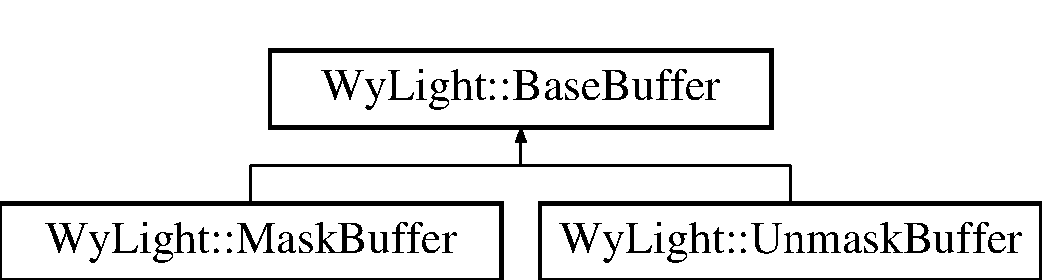
\includegraphics[height=2.000000cm]{class_wy_light_1_1_base_buffer}
\end{center}
\end{figure}
\subsection*{Public Member Functions}
\begin{DoxyCompactItemize}
\item 
\hyperlink{class_wy_light_1_1_base_buffer_a3a45cf0d57bbf72a0eb26fbc27b71b6c}{Base\-Buffer} (size\-\_\-t capacity)
\item 
virtual \hyperlink{class_wy_light_1_1_base_buffer_a0aa58a0961102462df6833aeb97a994f}{$\sim$\-Base\-Buffer} (void)
\item 
virtual void \hyperlink{class_wy_light_1_1_base_buffer_ad7c6538cc7136f71a96efe6d85c8ff8f}{Clear} (void)
\item 
const uint8\-\_\-t $\ast$ \hyperlink{class_wy_light_1_1_base_buffer_aae9c729bfa00ff4d4628da666b858c60}{Data} (void) const 
\item 
size\-\_\-t \hyperlink{class_wy_light_1_1_base_buffer_a6aa8fcfeaeeb093bce60211a3728337a}{Size} (void) const 
\end{DoxyCompactItemize}
\subsection*{Protected Member Functions}
\begin{DoxyCompactItemize}
\item 
void \hyperlink{class_wy_light_1_1_base_buffer_a528639672ade7ec49160c5297b246055}{Add\-Pure} (uint8\-\_\-t new\-Byte)
\end{DoxyCompactItemize}
\subsection*{Protected Attributes}
\begin{DoxyCompactItemize}
\item 
const size\-\_\-t \hyperlink{class_wy_light_1_1_base_buffer_a536a7f475b68dee906028913cab8799a}{m\-Capacity}
\item 
uint8\-\_\-t $\ast$ \hyperlink{class_wy_light_1_1_base_buffer_a724a04148d90146319fc11894d2ebd6e}{m\-Data}
\item 
size\-\_\-t \hyperlink{class_wy_light_1_1_base_buffer_ab36dd430b1e190e54ce338d3b98c1cbd}{m\-Length}
\item 
uint16\-\_\-t \hyperlink{class_wy_light_1_1_base_buffer_a084b781e48f372fc9d72ef95a7435d7a}{m\-Crc}
\end{DoxyCompactItemize}


\subsection{Constructor \& Destructor Documentation}
\hypertarget{class_wy_light_1_1_base_buffer_a3a45cf0d57bbf72a0eb26fbc27b71b6c}{\index{Wy\-Light\-::\-Base\-Buffer@{Wy\-Light\-::\-Base\-Buffer}!Base\-Buffer@{Base\-Buffer}}
\index{Base\-Buffer@{Base\-Buffer}!WyLight::BaseBuffer@{Wy\-Light\-::\-Base\-Buffer}}
\subsubsection[{Base\-Buffer}]{\setlength{\rightskip}{0pt plus 5cm}Wy\-Light\-::\-Base\-Buffer\-::\-Base\-Buffer (
\begin{DoxyParamCaption}
\item[{size\-\_\-t}]{capacity}
\end{DoxyParamCaption}
)\hspace{0.3cm}{\ttfamily [inline]}}}\label{class_wy_light_1_1_base_buffer_a3a45cf0d57bbf72a0eb26fbc27b71b6c}
\hypertarget{class_wy_light_1_1_base_buffer_a0aa58a0961102462df6833aeb97a994f}{\index{Wy\-Light\-::\-Base\-Buffer@{Wy\-Light\-::\-Base\-Buffer}!$\sim$\-Base\-Buffer@{$\sim$\-Base\-Buffer}}
\index{$\sim$\-Base\-Buffer@{$\sim$\-Base\-Buffer}!WyLight::BaseBuffer@{Wy\-Light\-::\-Base\-Buffer}}
\subsubsection[{$\sim$\-Base\-Buffer}]{\setlength{\rightskip}{0pt plus 5cm}virtual Wy\-Light\-::\-Base\-Buffer\-::$\sim$\-Base\-Buffer (
\begin{DoxyParamCaption}
\item[{void}]{}
\end{DoxyParamCaption}
)\hspace{0.3cm}{\ttfamily [inline]}, {\ttfamily [virtual]}}}\label{class_wy_light_1_1_base_buffer_a0aa58a0961102462df6833aeb97a994f}


\subsection{Member Function Documentation}
\hypertarget{class_wy_light_1_1_base_buffer_a528639672ade7ec49160c5297b246055}{\index{Wy\-Light\-::\-Base\-Buffer@{Wy\-Light\-::\-Base\-Buffer}!Add\-Pure@{Add\-Pure}}
\index{Add\-Pure@{Add\-Pure}!WyLight::BaseBuffer@{Wy\-Light\-::\-Base\-Buffer}}
\subsubsection[{Add\-Pure}]{\setlength{\rightskip}{0pt plus 5cm}void Wy\-Light\-::\-Base\-Buffer\-::\-Add\-Pure (
\begin{DoxyParamCaption}
\item[{uint8\-\_\-t}]{new\-Byte}
\end{DoxyParamCaption}
)\hspace{0.3cm}{\ttfamily [protected]}}}\label{class_wy_light_1_1_base_buffer_a528639672ade7ec49160c5297b246055}
\hypertarget{class_wy_light_1_1_base_buffer_ad7c6538cc7136f71a96efe6d85c8ff8f}{\index{Wy\-Light\-::\-Base\-Buffer@{Wy\-Light\-::\-Base\-Buffer}!Clear@{Clear}}
\index{Clear@{Clear}!WyLight::BaseBuffer@{Wy\-Light\-::\-Base\-Buffer}}
\subsubsection[{Clear}]{\setlength{\rightskip}{0pt plus 5cm}virtual void Wy\-Light\-::\-Base\-Buffer\-::\-Clear (
\begin{DoxyParamCaption}
\item[{void}]{}
\end{DoxyParamCaption}
)\hspace{0.3cm}{\ttfamily [inline]}, {\ttfamily [virtual]}}}\label{class_wy_light_1_1_base_buffer_ad7c6538cc7136f71a96efe6d85c8ff8f}


Reimplemented in \hyperlink{class_wy_light_1_1_unmask_buffer_a0d535dd72bf7759dc780e1341f30a75f}{Wy\-Light\-::\-Unmask\-Buffer}.

\hypertarget{class_wy_light_1_1_base_buffer_aae9c729bfa00ff4d4628da666b858c60}{\index{Wy\-Light\-::\-Base\-Buffer@{Wy\-Light\-::\-Base\-Buffer}!Data@{Data}}
\index{Data@{Data}!WyLight::BaseBuffer@{Wy\-Light\-::\-Base\-Buffer}}
\subsubsection[{Data}]{\setlength{\rightskip}{0pt plus 5cm}const uint8\-\_\-t$\ast$ Wy\-Light\-::\-Base\-Buffer\-::\-Data (
\begin{DoxyParamCaption}
\item[{void}]{}
\end{DoxyParamCaption}
) const\hspace{0.3cm}{\ttfamily [inline]}}}\label{class_wy_light_1_1_base_buffer_aae9c729bfa00ff4d4628da666b858c60}
\hypertarget{class_wy_light_1_1_base_buffer_a6aa8fcfeaeeb093bce60211a3728337a}{\index{Wy\-Light\-::\-Base\-Buffer@{Wy\-Light\-::\-Base\-Buffer}!Size@{Size}}
\index{Size@{Size}!WyLight::BaseBuffer@{Wy\-Light\-::\-Base\-Buffer}}
\subsubsection[{Size}]{\setlength{\rightskip}{0pt plus 5cm}size\-\_\-t Wy\-Light\-::\-Base\-Buffer\-::\-Size (
\begin{DoxyParamCaption}
\item[{void}]{}
\end{DoxyParamCaption}
) const\hspace{0.3cm}{\ttfamily [inline]}}}\label{class_wy_light_1_1_base_buffer_a6aa8fcfeaeeb093bce60211a3728337a}


\subsection{Member Data Documentation}
\hypertarget{class_wy_light_1_1_base_buffer_a536a7f475b68dee906028913cab8799a}{\index{Wy\-Light\-::\-Base\-Buffer@{Wy\-Light\-::\-Base\-Buffer}!m\-Capacity@{m\-Capacity}}
\index{m\-Capacity@{m\-Capacity}!WyLight::BaseBuffer@{Wy\-Light\-::\-Base\-Buffer}}
\subsubsection[{m\-Capacity}]{\setlength{\rightskip}{0pt plus 5cm}const size\-\_\-t Wy\-Light\-::\-Base\-Buffer\-::m\-Capacity\hspace{0.3cm}{\ttfamily [protected]}}}\label{class_wy_light_1_1_base_buffer_a536a7f475b68dee906028913cab8799a}
\hypertarget{class_wy_light_1_1_base_buffer_a084b781e48f372fc9d72ef95a7435d7a}{\index{Wy\-Light\-::\-Base\-Buffer@{Wy\-Light\-::\-Base\-Buffer}!m\-Crc@{m\-Crc}}
\index{m\-Crc@{m\-Crc}!WyLight::BaseBuffer@{Wy\-Light\-::\-Base\-Buffer}}
\subsubsection[{m\-Crc}]{\setlength{\rightskip}{0pt plus 5cm}uint16\-\_\-t Wy\-Light\-::\-Base\-Buffer\-::m\-Crc\hspace{0.3cm}{\ttfamily [protected]}}}\label{class_wy_light_1_1_base_buffer_a084b781e48f372fc9d72ef95a7435d7a}
\hypertarget{class_wy_light_1_1_base_buffer_a724a04148d90146319fc11894d2ebd6e}{\index{Wy\-Light\-::\-Base\-Buffer@{Wy\-Light\-::\-Base\-Buffer}!m\-Data@{m\-Data}}
\index{m\-Data@{m\-Data}!WyLight::BaseBuffer@{Wy\-Light\-::\-Base\-Buffer}}
\subsubsection[{m\-Data}]{\setlength{\rightskip}{0pt plus 5cm}uint8\-\_\-t$\ast$ Wy\-Light\-::\-Base\-Buffer\-::m\-Data\hspace{0.3cm}{\ttfamily [protected]}}}\label{class_wy_light_1_1_base_buffer_a724a04148d90146319fc11894d2ebd6e}
\hypertarget{class_wy_light_1_1_base_buffer_ab36dd430b1e190e54ce338d3b98c1cbd}{\index{Wy\-Light\-::\-Base\-Buffer@{Wy\-Light\-::\-Base\-Buffer}!m\-Length@{m\-Length}}
\index{m\-Length@{m\-Length}!WyLight::BaseBuffer@{Wy\-Light\-::\-Base\-Buffer}}
\subsubsection[{m\-Length}]{\setlength{\rightskip}{0pt plus 5cm}size\-\_\-t Wy\-Light\-::\-Base\-Buffer\-::m\-Length\hspace{0.3cm}{\ttfamily [protected]}}}\label{class_wy_light_1_1_base_buffer_ab36dd430b1e190e54ce338d3b98c1cbd}


The documentation for this class was generated from the following file\-:\begin{DoxyCompactItemize}
\item 
library/\hyperlink{_mask_buffer_8h}{Mask\-Buffer.\-h}\end{DoxyCompactItemize}

\hypertarget{struct_wy_light_1_1_bl_address_request}{\section{Wy\-Light\-:\-:Bl\-Address\-Request Struct Reference}
\label{struct_wy_light_1_1_bl_address_request}\index{Wy\-Light\-::\-Bl\-Address\-Request@{Wy\-Light\-::\-Bl\-Address\-Request}}
}


{\ttfamily \#include $<$Bl\-Request.\-h$>$}

Inheritance diagram for Wy\-Light\-:\-:Bl\-Address\-Request\-:\begin{figure}[H]
\begin{center}
\leavevmode
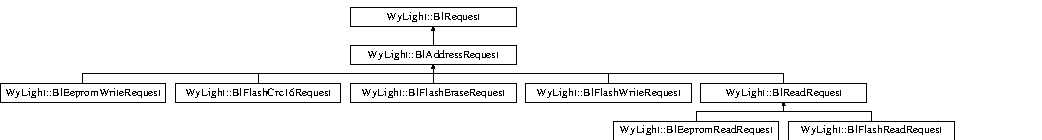
\includegraphics[height=1.885522cm]{struct_wy_light_1_1_bl_address_request}
\end{center}
\end{figure}
\subsection*{Public Member Functions}
\begin{DoxyCompactItemize}
\item 
\hyperlink{struct_wy_light_1_1_bl_address_request_a0a8d89736463ad09d739bff4bd773a45}{Bl\-Address\-Request} (size\-\_\-t size, unsigned char cmd)
\item 
virtual void \hyperlink{struct_wy_light_1_1_bl_address_request_afa463bc5ccf900bd979f547fbb39d7a7}{Set\-Address} (unsigned int address)
\end{DoxyCompactItemize}
\subsection*{Public Attributes}
\begin{DoxyCompactItemize}
\item 
unsigned char \hyperlink{struct_wy_light_1_1_bl_address_request_a27582cf3b7f0dcd17edd1ea640e0b90e}{address\-Low}
\item 
unsigned char \hyperlink{struct_wy_light_1_1_bl_address_request_a3e050aa490810811fbe60e04d4cba538}{address\-High}
\item 
unsigned char \hyperlink{struct_wy_light_1_1_bl_address_request_a1e4b9c78761aba98a236dd9358350a33}{address\-U}
\item 
const unsigned char \hyperlink{struct_wy_light_1_1_bl_address_request_a2974213d2ae8d71fb5948e4623d422c9}{zero}
\end{DoxyCompactItemize}


\subsection{Constructor \& Destructor Documentation}
\hypertarget{struct_wy_light_1_1_bl_address_request_a0a8d89736463ad09d739bff4bd773a45}{\index{Wy\-Light\-::\-Bl\-Address\-Request@{Wy\-Light\-::\-Bl\-Address\-Request}!Bl\-Address\-Request@{Bl\-Address\-Request}}
\index{Bl\-Address\-Request@{Bl\-Address\-Request}!WyLight::BlAddressRequest@{Wy\-Light\-::\-Bl\-Address\-Request}}
\subsubsection[{Bl\-Address\-Request}]{\setlength{\rightskip}{0pt plus 5cm}Wy\-Light\-::\-Bl\-Address\-Request\-::\-Bl\-Address\-Request (
\begin{DoxyParamCaption}
\item[{size\-\_\-t}]{size, }
\item[{unsigned char}]{cmd}
\end{DoxyParamCaption}
)\hspace{0.3cm}{\ttfamily [inline]}}}\label{struct_wy_light_1_1_bl_address_request_a0a8d89736463ad09d739bff4bd773a45}


\subsection{Member Function Documentation}
\hypertarget{struct_wy_light_1_1_bl_address_request_afa463bc5ccf900bd979f547fbb39d7a7}{\index{Wy\-Light\-::\-Bl\-Address\-Request@{Wy\-Light\-::\-Bl\-Address\-Request}!Set\-Address@{Set\-Address}}
\index{Set\-Address@{Set\-Address}!WyLight::BlAddressRequest@{Wy\-Light\-::\-Bl\-Address\-Request}}
\subsubsection[{Set\-Address}]{\setlength{\rightskip}{0pt plus 5cm}virtual void Wy\-Light\-::\-Bl\-Address\-Request\-::\-Set\-Address (
\begin{DoxyParamCaption}
\item[{unsigned int}]{address}
\end{DoxyParamCaption}
)\hspace{0.3cm}{\ttfamily [inline]}, {\ttfamily [virtual]}}}\label{struct_wy_light_1_1_bl_address_request_afa463bc5ccf900bd979f547fbb39d7a7}


\subsection{Member Data Documentation}
\hypertarget{struct_wy_light_1_1_bl_address_request_a3e050aa490810811fbe60e04d4cba538}{\index{Wy\-Light\-::\-Bl\-Address\-Request@{Wy\-Light\-::\-Bl\-Address\-Request}!address\-High@{address\-High}}
\index{address\-High@{address\-High}!WyLight::BlAddressRequest@{Wy\-Light\-::\-Bl\-Address\-Request}}
\subsubsection[{address\-High}]{\setlength{\rightskip}{0pt plus 5cm}unsigned char Wy\-Light\-::\-Bl\-Address\-Request\-::address\-High}}\label{struct_wy_light_1_1_bl_address_request_a3e050aa490810811fbe60e04d4cba538}
\hypertarget{struct_wy_light_1_1_bl_address_request_a27582cf3b7f0dcd17edd1ea640e0b90e}{\index{Wy\-Light\-::\-Bl\-Address\-Request@{Wy\-Light\-::\-Bl\-Address\-Request}!address\-Low@{address\-Low}}
\index{address\-Low@{address\-Low}!WyLight::BlAddressRequest@{Wy\-Light\-::\-Bl\-Address\-Request}}
\subsubsection[{address\-Low}]{\setlength{\rightskip}{0pt plus 5cm}unsigned char Wy\-Light\-::\-Bl\-Address\-Request\-::address\-Low}}\label{struct_wy_light_1_1_bl_address_request_a27582cf3b7f0dcd17edd1ea640e0b90e}
\hypertarget{struct_wy_light_1_1_bl_address_request_a1e4b9c78761aba98a236dd9358350a33}{\index{Wy\-Light\-::\-Bl\-Address\-Request@{Wy\-Light\-::\-Bl\-Address\-Request}!address\-U@{address\-U}}
\index{address\-U@{address\-U}!WyLight::BlAddressRequest@{Wy\-Light\-::\-Bl\-Address\-Request}}
\subsubsection[{address\-U}]{\setlength{\rightskip}{0pt plus 5cm}unsigned char Wy\-Light\-::\-Bl\-Address\-Request\-::address\-U}}\label{struct_wy_light_1_1_bl_address_request_a1e4b9c78761aba98a236dd9358350a33}
\hypertarget{struct_wy_light_1_1_bl_address_request_a2974213d2ae8d71fb5948e4623d422c9}{\index{Wy\-Light\-::\-Bl\-Address\-Request@{Wy\-Light\-::\-Bl\-Address\-Request}!zero@{zero}}
\index{zero@{zero}!WyLight::BlAddressRequest@{Wy\-Light\-::\-Bl\-Address\-Request}}
\subsubsection[{zero}]{\setlength{\rightskip}{0pt plus 5cm}const unsigned char Wy\-Light\-::\-Bl\-Address\-Request\-::zero}}\label{struct_wy_light_1_1_bl_address_request_a2974213d2ae8d71fb5948e4623d422c9}


The documentation for this struct was generated from the following file\-:\begin{DoxyCompactItemize}
\item 
library/\hyperlink{_bl_request_8h}{Bl\-Request.\-h}\end{DoxyCompactItemize}

\hypertarget{struct_wy_light_1_1_bl_eeprom_read_request}{\section{Wy\-Light\-:\-:Bl\-Eeprom\-Read\-Request Struct Reference}
\label{struct_wy_light_1_1_bl_eeprom_read_request}\index{Wy\-Light\-::\-Bl\-Eeprom\-Read\-Request@{Wy\-Light\-::\-Bl\-Eeprom\-Read\-Request}}
}


{\ttfamily \#include $<$Bl\-Request.\-h$>$}

Inheritance diagram for Wy\-Light\-:\-:Bl\-Eeprom\-Read\-Request\-:\begin{figure}[H]
\begin{center}
\leavevmode
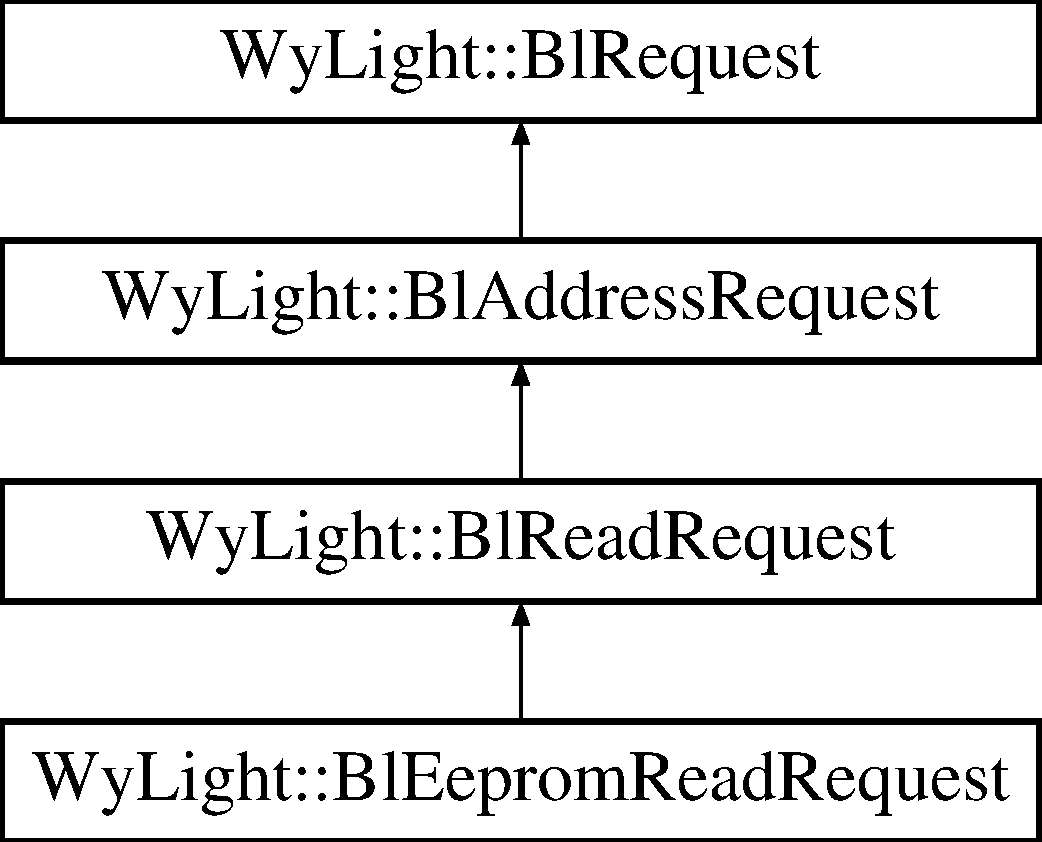
\includegraphics[height=4.000000cm]{struct_wy_light_1_1_bl_eeprom_read_request}
\end{center}
\end{figure}
\subsection*{Public Member Functions}
\begin{DoxyCompactItemize}
\item 
\hyperlink{struct_wy_light_1_1_bl_eeprom_read_request_aa303eb606e85418857e81cacbf3ef8da}{Bl\-Eeprom\-Read\-Request} ()
\end{DoxyCompactItemize}
\subsection*{Additional Inherited Members}


\subsection{Constructor \& Destructor Documentation}
\hypertarget{struct_wy_light_1_1_bl_eeprom_read_request_aa303eb606e85418857e81cacbf3ef8da}{\index{Wy\-Light\-::\-Bl\-Eeprom\-Read\-Request@{Wy\-Light\-::\-Bl\-Eeprom\-Read\-Request}!Bl\-Eeprom\-Read\-Request@{Bl\-Eeprom\-Read\-Request}}
\index{Bl\-Eeprom\-Read\-Request@{Bl\-Eeprom\-Read\-Request}!WyLight::BlEepromReadRequest@{Wy\-Light\-::\-Bl\-Eeprom\-Read\-Request}}
\subsubsection[{Bl\-Eeprom\-Read\-Request}]{\setlength{\rightskip}{0pt plus 5cm}Wy\-Light\-::\-Bl\-Eeprom\-Read\-Request\-::\-Bl\-Eeprom\-Read\-Request (
\begin{DoxyParamCaption}
{}
\end{DoxyParamCaption}
)\hspace{0.3cm}{\ttfamily [inline]}}}\label{struct_wy_light_1_1_bl_eeprom_read_request_aa303eb606e85418857e81cacbf3ef8da}


The documentation for this struct was generated from the following file\-:\begin{DoxyCompactItemize}
\item 
library/\hyperlink{_bl_request_8h}{Bl\-Request.\-h}\end{DoxyCompactItemize}

\hypertarget{struct_wy_light_1_1_bl_eeprom_write_request}{\section{Wy\-Light\-:\-:Bl\-Eeprom\-Write\-Request Struct Reference}
\label{struct_wy_light_1_1_bl_eeprom_write_request}\index{Wy\-Light\-::\-Bl\-Eeprom\-Write\-Request@{Wy\-Light\-::\-Bl\-Eeprom\-Write\-Request}}
}


{\ttfamily \#include $<$Bl\-Request.\-h$>$}

Inheritance diagram for Wy\-Light\-:\-:Bl\-Eeprom\-Write\-Request\-:\begin{figure}[H]
\begin{center}
\leavevmode
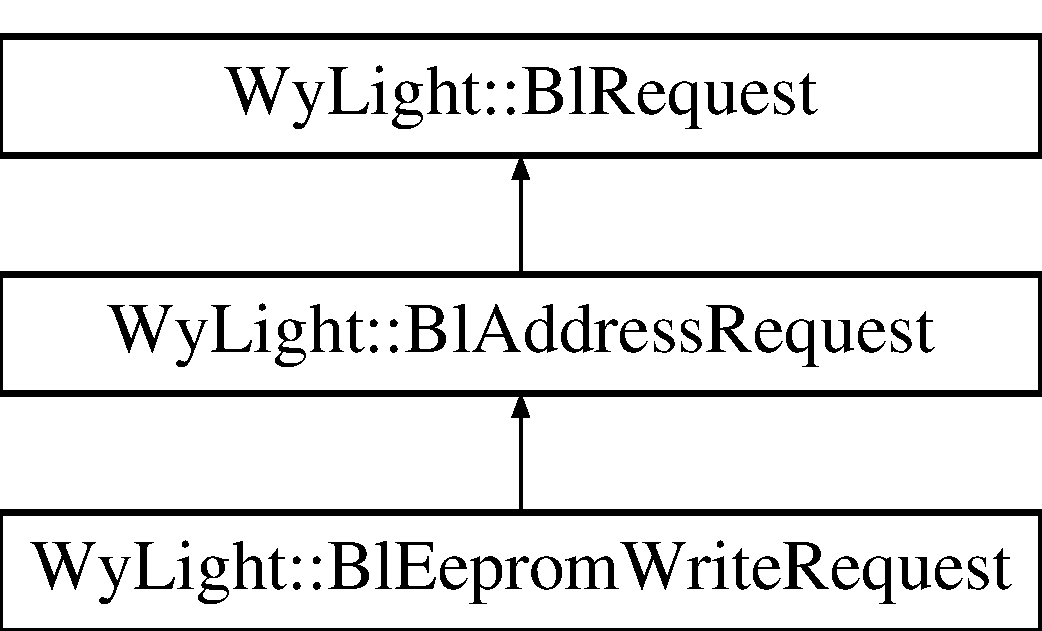
\includegraphics[height=3.000000cm]{struct_wy_light_1_1_bl_eeprom_write_request}
\end{center}
\end{figure}
\subsection*{Public Member Functions}
\begin{DoxyCompactItemize}
\item 
\hyperlink{struct_wy_light_1_1_bl_eeprom_write_request_aa0b5642cd84432219d60b65f02ba7ae9}{Bl\-Eeprom\-Write\-Request} ()
\item 
void \hyperlink{struct_wy_light_1_1_bl_eeprom_write_request_aefd927d0a951a3922c920eae122577b1}{Set\-Data} (unsigned int address, const uint8\-\_\-t $\ast$p\-Data, size\-\_\-t num\-Bytes)
\end{DoxyCompactItemize}
\subsection*{Public Attributes}
\begin{DoxyCompactItemize}
\item 
unsigned char \hyperlink{struct_wy_light_1_1_bl_eeprom_write_request_a70fa73997362e6e765c9f2bdfaf67aef}{num\-Bytes\-Low}
\item 
unsigned char \hyperlink{struct_wy_light_1_1_bl_eeprom_write_request_a241263672f5229fea259fa45e8cafae0}{num\-Bytes\-High}
\item 
unsigned char \hyperlink{struct_wy_light_1_1_bl_eeprom_write_request_ae5efc27e17509d1ba2655f964f7a2917}{payload} \mbox{[}\hyperlink{_bl_request_8h_a5f45dd63fc17090ece1b40b668195185}{E\-E\-P\-R\-O\-M\-\_\-\-W\-R\-I\-T\-E\-\_\-\-B\-L\-O\-C\-K\-S\-I\-Z\-E}\mbox{]}
\end{DoxyCompactItemize}


\subsection{Constructor \& Destructor Documentation}
\hypertarget{struct_wy_light_1_1_bl_eeprom_write_request_aa0b5642cd84432219d60b65f02ba7ae9}{\index{Wy\-Light\-::\-Bl\-Eeprom\-Write\-Request@{Wy\-Light\-::\-Bl\-Eeprom\-Write\-Request}!Bl\-Eeprom\-Write\-Request@{Bl\-Eeprom\-Write\-Request}}
\index{Bl\-Eeprom\-Write\-Request@{Bl\-Eeprom\-Write\-Request}!WyLight::BlEepromWriteRequest@{Wy\-Light\-::\-Bl\-Eeprom\-Write\-Request}}
\subsubsection[{Bl\-Eeprom\-Write\-Request}]{\setlength{\rightskip}{0pt plus 5cm}Wy\-Light\-::\-Bl\-Eeprom\-Write\-Request\-::\-Bl\-Eeprom\-Write\-Request (
\begin{DoxyParamCaption}
{}
\end{DoxyParamCaption}
)\hspace{0.3cm}{\ttfamily [inline]}}}\label{struct_wy_light_1_1_bl_eeprom_write_request_aa0b5642cd84432219d60b65f02ba7ae9}


\subsection{Member Function Documentation}
\hypertarget{struct_wy_light_1_1_bl_eeprom_write_request_aefd927d0a951a3922c920eae122577b1}{\index{Wy\-Light\-::\-Bl\-Eeprom\-Write\-Request@{Wy\-Light\-::\-Bl\-Eeprom\-Write\-Request}!Set\-Data@{Set\-Data}}
\index{Set\-Data@{Set\-Data}!WyLight::BlEepromWriteRequest@{Wy\-Light\-::\-Bl\-Eeprom\-Write\-Request}}
\subsubsection[{Set\-Data}]{\setlength{\rightskip}{0pt plus 5cm}void Wy\-Light\-::\-Bl\-Eeprom\-Write\-Request\-::\-Set\-Data (
\begin{DoxyParamCaption}
\item[{unsigned int}]{address, }
\item[{const uint8\-\_\-t $\ast$}]{p\-Data, }
\item[{size\-\_\-t}]{num\-Bytes}
\end{DoxyParamCaption}
)\hspace{0.3cm}{\ttfamily [inline]}}}\label{struct_wy_light_1_1_bl_eeprom_write_request_aefd927d0a951a3922c920eae122577b1}


\subsection{Member Data Documentation}
\hypertarget{struct_wy_light_1_1_bl_eeprom_write_request_a241263672f5229fea259fa45e8cafae0}{\index{Wy\-Light\-::\-Bl\-Eeprom\-Write\-Request@{Wy\-Light\-::\-Bl\-Eeprom\-Write\-Request}!num\-Bytes\-High@{num\-Bytes\-High}}
\index{num\-Bytes\-High@{num\-Bytes\-High}!WyLight::BlEepromWriteRequest@{Wy\-Light\-::\-Bl\-Eeprom\-Write\-Request}}
\subsubsection[{num\-Bytes\-High}]{\setlength{\rightskip}{0pt plus 5cm}unsigned char Wy\-Light\-::\-Bl\-Eeprom\-Write\-Request\-::num\-Bytes\-High}}\label{struct_wy_light_1_1_bl_eeprom_write_request_a241263672f5229fea259fa45e8cafae0}
\hypertarget{struct_wy_light_1_1_bl_eeprom_write_request_a70fa73997362e6e765c9f2bdfaf67aef}{\index{Wy\-Light\-::\-Bl\-Eeprom\-Write\-Request@{Wy\-Light\-::\-Bl\-Eeprom\-Write\-Request}!num\-Bytes\-Low@{num\-Bytes\-Low}}
\index{num\-Bytes\-Low@{num\-Bytes\-Low}!WyLight::BlEepromWriteRequest@{Wy\-Light\-::\-Bl\-Eeprom\-Write\-Request}}
\subsubsection[{num\-Bytes\-Low}]{\setlength{\rightskip}{0pt plus 5cm}unsigned char Wy\-Light\-::\-Bl\-Eeprom\-Write\-Request\-::num\-Bytes\-Low}}\label{struct_wy_light_1_1_bl_eeprom_write_request_a70fa73997362e6e765c9f2bdfaf67aef}
\hypertarget{struct_wy_light_1_1_bl_eeprom_write_request_ae5efc27e17509d1ba2655f964f7a2917}{\index{Wy\-Light\-::\-Bl\-Eeprom\-Write\-Request@{Wy\-Light\-::\-Bl\-Eeprom\-Write\-Request}!payload@{payload}}
\index{payload@{payload}!WyLight::BlEepromWriteRequest@{Wy\-Light\-::\-Bl\-Eeprom\-Write\-Request}}
\subsubsection[{payload}]{\setlength{\rightskip}{0pt plus 5cm}unsigned char Wy\-Light\-::\-Bl\-Eeprom\-Write\-Request\-::payload\mbox{[}{\bf E\-E\-P\-R\-O\-M\-\_\-\-W\-R\-I\-T\-E\-\_\-\-B\-L\-O\-C\-K\-S\-I\-Z\-E}\mbox{]}}}\label{struct_wy_light_1_1_bl_eeprom_write_request_ae5efc27e17509d1ba2655f964f7a2917}


The documentation for this struct was generated from the following file\-:\begin{DoxyCompactItemize}
\item 
library/\hyperlink{_bl_request_8h}{Bl\-Request.\-h}\end{DoxyCompactItemize}

\hypertarget{struct_wy_light_1_1_bl_flash_crc16_request}{\section{Wy\-Light\-:\-:Bl\-Flash\-Crc16\-Request Struct Reference}
\label{struct_wy_light_1_1_bl_flash_crc16_request}\index{Wy\-Light\-::\-Bl\-Flash\-Crc16\-Request@{Wy\-Light\-::\-Bl\-Flash\-Crc16\-Request}}
}


{\ttfamily \#include $<$Bl\-Request.\-h$>$}

Inheritance diagram for Wy\-Light\-:\-:Bl\-Flash\-Crc16\-Request\-:\begin{figure}[H]
\begin{center}
\leavevmode
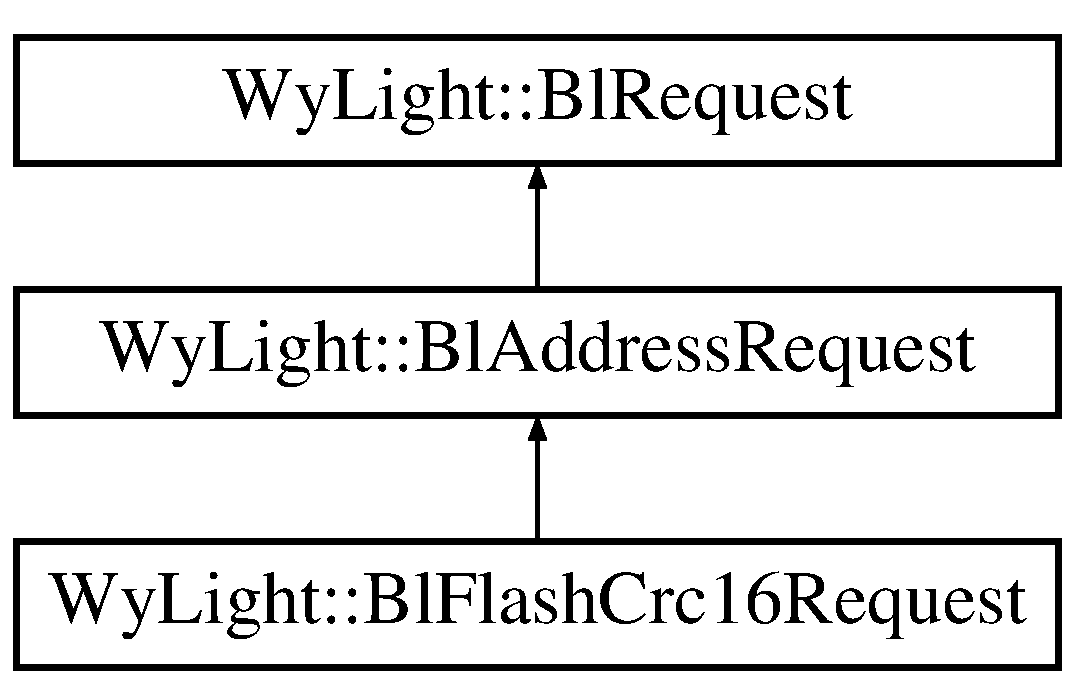
\includegraphics[height=3.000000cm]{struct_wy_light_1_1_bl_flash_crc16_request}
\end{center}
\end{figure}
\subsection*{Public Member Functions}
\begin{DoxyCompactItemize}
\item 
\hyperlink{struct_wy_light_1_1_bl_flash_crc16_request_a532917f2e6d2a7c3b44c9d9f6691bcfa}{Bl\-Flash\-Crc16\-Request} (uint32\-\_\-t address, uint16\-\_\-t num\-Blocks)
\item 
virtual bool \hyperlink{struct_wy_light_1_1_bl_flash_crc16_request_a7a3a14722ed86688b5992f84089adc3c}{Check\-Crc} () const 
\end{DoxyCompactItemize}
\subsection*{Public Attributes}
\begin{DoxyCompactItemize}
\item 
uint8\-\_\-t \hyperlink{struct_wy_light_1_1_bl_flash_crc16_request_ae203ed160c58cf31e6395fd3c1e7560b}{num\-Blocks\-Low}
\item 
uint8\-\_\-t \hyperlink{struct_wy_light_1_1_bl_flash_crc16_request_a336dd15d053c5e7330a638de12141b35}{num\-Blocks\-High}
\end{DoxyCompactItemize}


\subsection{Constructor \& Destructor Documentation}
\hypertarget{struct_wy_light_1_1_bl_flash_crc16_request_a532917f2e6d2a7c3b44c9d9f6691bcfa}{\index{Wy\-Light\-::\-Bl\-Flash\-Crc16\-Request@{Wy\-Light\-::\-Bl\-Flash\-Crc16\-Request}!Bl\-Flash\-Crc16\-Request@{Bl\-Flash\-Crc16\-Request}}
\index{Bl\-Flash\-Crc16\-Request@{Bl\-Flash\-Crc16\-Request}!WyLight::BlFlashCrc16Request@{Wy\-Light\-::\-Bl\-Flash\-Crc16\-Request}}
\subsubsection[{Bl\-Flash\-Crc16\-Request}]{\setlength{\rightskip}{0pt plus 5cm}Wy\-Light\-::\-Bl\-Flash\-Crc16\-Request\-::\-Bl\-Flash\-Crc16\-Request (
\begin{DoxyParamCaption}
\item[{uint32\-\_\-t}]{address, }
\item[{uint16\-\_\-t}]{num\-Blocks}
\end{DoxyParamCaption}
)\hspace{0.3cm}{\ttfamily [inline]}}}\label{struct_wy_light_1_1_bl_flash_crc16_request_a532917f2e6d2a7c3b44c9d9f6691bcfa}


\subsection{Member Function Documentation}
\hypertarget{struct_wy_light_1_1_bl_flash_crc16_request_a7a3a14722ed86688b5992f84089adc3c}{\index{Wy\-Light\-::\-Bl\-Flash\-Crc16\-Request@{Wy\-Light\-::\-Bl\-Flash\-Crc16\-Request}!Check\-Crc@{Check\-Crc}}
\index{Check\-Crc@{Check\-Crc}!WyLight::BlFlashCrc16Request@{Wy\-Light\-::\-Bl\-Flash\-Crc16\-Request}}
\subsubsection[{Check\-Crc}]{\setlength{\rightskip}{0pt plus 5cm}virtual bool Wy\-Light\-::\-Bl\-Flash\-Crc16\-Request\-::\-Check\-Crc (
\begin{DoxyParamCaption}
{}
\end{DoxyParamCaption}
) const\hspace{0.3cm}{\ttfamily [inline]}, {\ttfamily [virtual]}}}\label{struct_wy_light_1_1_bl_flash_crc16_request_a7a3a14722ed86688b5992f84089adc3c}


Reimplemented from \hyperlink{struct_wy_light_1_1_bl_request_a35e6aeaab96cce48c4dcc2f63eb920c4}{Wy\-Light\-::\-Bl\-Request}.



\subsection{Member Data Documentation}
\hypertarget{struct_wy_light_1_1_bl_flash_crc16_request_a336dd15d053c5e7330a638de12141b35}{\index{Wy\-Light\-::\-Bl\-Flash\-Crc16\-Request@{Wy\-Light\-::\-Bl\-Flash\-Crc16\-Request}!num\-Blocks\-High@{num\-Blocks\-High}}
\index{num\-Blocks\-High@{num\-Blocks\-High}!WyLight::BlFlashCrc16Request@{Wy\-Light\-::\-Bl\-Flash\-Crc16\-Request}}
\subsubsection[{num\-Blocks\-High}]{\setlength{\rightskip}{0pt plus 5cm}uint8\-\_\-t Wy\-Light\-::\-Bl\-Flash\-Crc16\-Request\-::num\-Blocks\-High}}\label{struct_wy_light_1_1_bl_flash_crc16_request_a336dd15d053c5e7330a638de12141b35}
\hypertarget{struct_wy_light_1_1_bl_flash_crc16_request_ae203ed160c58cf31e6395fd3c1e7560b}{\index{Wy\-Light\-::\-Bl\-Flash\-Crc16\-Request@{Wy\-Light\-::\-Bl\-Flash\-Crc16\-Request}!num\-Blocks\-Low@{num\-Blocks\-Low}}
\index{num\-Blocks\-Low@{num\-Blocks\-Low}!WyLight::BlFlashCrc16Request@{Wy\-Light\-::\-Bl\-Flash\-Crc16\-Request}}
\subsubsection[{num\-Blocks\-Low}]{\setlength{\rightskip}{0pt plus 5cm}uint8\-\_\-t Wy\-Light\-::\-Bl\-Flash\-Crc16\-Request\-::num\-Blocks\-Low}}\label{struct_wy_light_1_1_bl_flash_crc16_request_ae203ed160c58cf31e6395fd3c1e7560b}


The documentation for this struct was generated from the following file\-:\begin{DoxyCompactItemize}
\item 
library/\hyperlink{_bl_request_8h}{Bl\-Request.\-h}\end{DoxyCompactItemize}

\hypertarget{struct_wy_light_1_1_bl_flash_erase_request}{\section{Wy\-Light\-:\-:Bl\-Flash\-Erase\-Request Struct Reference}
\label{struct_wy_light_1_1_bl_flash_erase_request}\index{Wy\-Light\-::\-Bl\-Flash\-Erase\-Request@{Wy\-Light\-::\-Bl\-Flash\-Erase\-Request}}
}


{\ttfamily \#include $<$Bl\-Request.\-h$>$}

Inheritance diagram for Wy\-Light\-:\-:Bl\-Flash\-Erase\-Request\-:\begin{figure}[H]
\begin{center}
\leavevmode
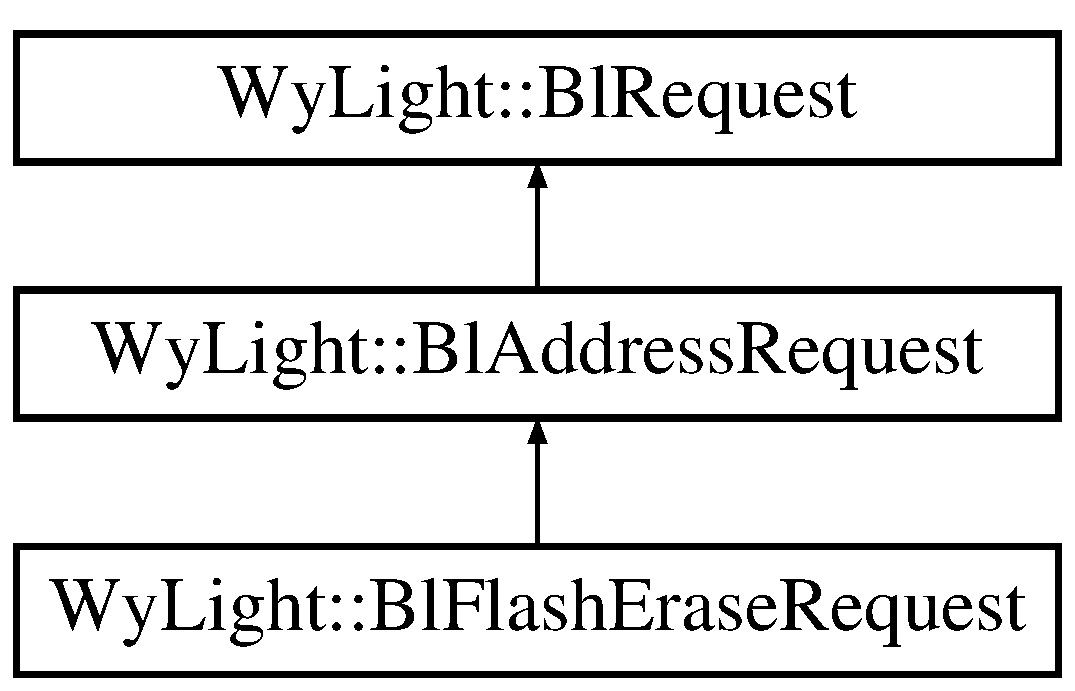
\includegraphics[height=3.000000cm]{struct_wy_light_1_1_bl_flash_erase_request}
\end{center}
\end{figure}
\subsection*{Public Member Functions}
\begin{DoxyCompactItemize}
\item 
\hyperlink{struct_wy_light_1_1_bl_flash_erase_request_ad069728b703ecc3830c589475664cf22}{Bl\-Flash\-Erase\-Request} (uint32\-\_\-t address, uint8\-\_\-t num\-Flash\-Pages)
\end{DoxyCompactItemize}
\subsection*{Public Attributes}
\begin{DoxyCompactItemize}
\item 
const unsigned char \hyperlink{struct_wy_light_1_1_bl_flash_erase_request_a4e95486e9c8f309b066e8251fc1d7593}{num\-Pages}
\end{DoxyCompactItemize}


\subsection{Constructor \& Destructor Documentation}
\hypertarget{struct_wy_light_1_1_bl_flash_erase_request_ad069728b703ecc3830c589475664cf22}{\index{Wy\-Light\-::\-Bl\-Flash\-Erase\-Request@{Wy\-Light\-::\-Bl\-Flash\-Erase\-Request}!Bl\-Flash\-Erase\-Request@{Bl\-Flash\-Erase\-Request}}
\index{Bl\-Flash\-Erase\-Request@{Bl\-Flash\-Erase\-Request}!WyLight::BlFlashEraseRequest@{Wy\-Light\-::\-Bl\-Flash\-Erase\-Request}}
\subsubsection[{Bl\-Flash\-Erase\-Request}]{\setlength{\rightskip}{0pt plus 5cm}Wy\-Light\-::\-Bl\-Flash\-Erase\-Request\-::\-Bl\-Flash\-Erase\-Request (
\begin{DoxyParamCaption}
\item[{uint32\-\_\-t}]{address, }
\item[{uint8\-\_\-t}]{num\-Flash\-Pages}
\end{DoxyParamCaption}
)\hspace{0.3cm}{\ttfamily [inline]}}}\label{struct_wy_light_1_1_bl_flash_erase_request_ad069728b703ecc3830c589475664cf22}


\subsection{Member Data Documentation}
\hypertarget{struct_wy_light_1_1_bl_flash_erase_request_a4e95486e9c8f309b066e8251fc1d7593}{\index{Wy\-Light\-::\-Bl\-Flash\-Erase\-Request@{Wy\-Light\-::\-Bl\-Flash\-Erase\-Request}!num\-Pages@{num\-Pages}}
\index{num\-Pages@{num\-Pages}!WyLight::BlFlashEraseRequest@{Wy\-Light\-::\-Bl\-Flash\-Erase\-Request}}
\subsubsection[{num\-Pages}]{\setlength{\rightskip}{0pt plus 5cm}const unsigned char Wy\-Light\-::\-Bl\-Flash\-Erase\-Request\-::num\-Pages}}\label{struct_wy_light_1_1_bl_flash_erase_request_a4e95486e9c8f309b066e8251fc1d7593}


The documentation for this struct was generated from the following file\-:\begin{DoxyCompactItemize}
\item 
library/\hyperlink{_bl_request_8h}{Bl\-Request.\-h}\end{DoxyCompactItemize}

\hypertarget{struct_wy_light_1_1_bl_flash_read_request}{\section{Wy\-Light\-:\-:Bl\-Flash\-Read\-Request Struct Reference}
\label{struct_wy_light_1_1_bl_flash_read_request}\index{Wy\-Light\-::\-Bl\-Flash\-Read\-Request@{Wy\-Light\-::\-Bl\-Flash\-Read\-Request}}
}


{\ttfamily \#include $<$Bl\-Request.\-h$>$}

Inheritance diagram for Wy\-Light\-:\-:Bl\-Flash\-Read\-Request\-:\begin{figure}[H]
\begin{center}
\leavevmode
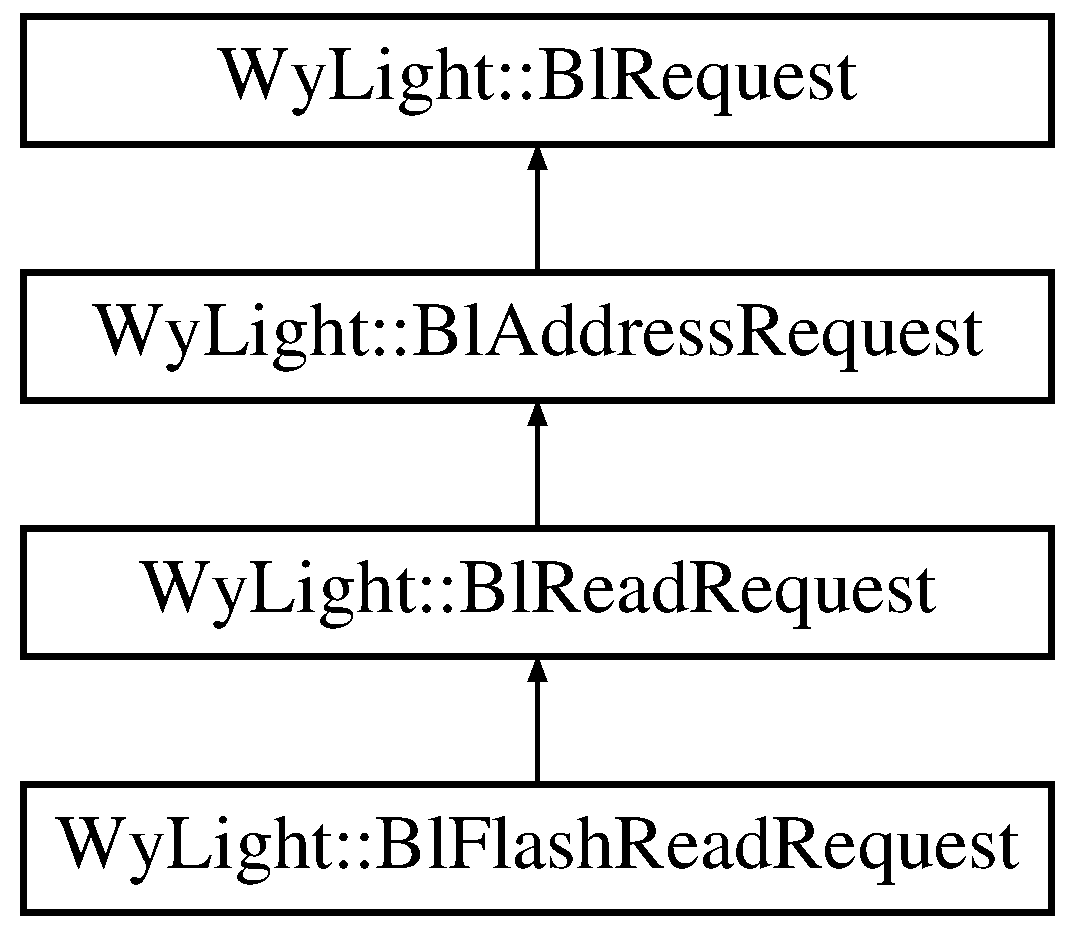
\includegraphics[height=4.000000cm]{struct_wy_light_1_1_bl_flash_read_request}
\end{center}
\end{figure}
\subsection*{Public Member Functions}
\begin{DoxyCompactItemize}
\item 
\hyperlink{struct_wy_light_1_1_bl_flash_read_request_aa13af15bd17ee01c4f9af313211299e8}{Bl\-Flash\-Read\-Request} ()
\end{DoxyCompactItemize}
\subsection*{Additional Inherited Members}


\subsection{Constructor \& Destructor Documentation}
\hypertarget{struct_wy_light_1_1_bl_flash_read_request_aa13af15bd17ee01c4f9af313211299e8}{\index{Wy\-Light\-::\-Bl\-Flash\-Read\-Request@{Wy\-Light\-::\-Bl\-Flash\-Read\-Request}!Bl\-Flash\-Read\-Request@{Bl\-Flash\-Read\-Request}}
\index{Bl\-Flash\-Read\-Request@{Bl\-Flash\-Read\-Request}!WyLight::BlFlashReadRequest@{Wy\-Light\-::\-Bl\-Flash\-Read\-Request}}
\subsubsection[{Bl\-Flash\-Read\-Request}]{\setlength{\rightskip}{0pt plus 5cm}Wy\-Light\-::\-Bl\-Flash\-Read\-Request\-::\-Bl\-Flash\-Read\-Request (
\begin{DoxyParamCaption}
{}
\end{DoxyParamCaption}
)\hspace{0.3cm}{\ttfamily [inline]}}}\label{struct_wy_light_1_1_bl_flash_read_request_aa13af15bd17ee01c4f9af313211299e8}


The documentation for this struct was generated from the following file\-:\begin{DoxyCompactItemize}
\item 
library/\hyperlink{_bl_request_8h}{Bl\-Request.\-h}\end{DoxyCompactItemize}

\hypertarget{struct_wy_light_1_1_bl_flash_write_request}{\section{Wy\-Light\-:\-:Bl\-Flash\-Write\-Request Struct Reference}
\label{struct_wy_light_1_1_bl_flash_write_request}\index{Wy\-Light\-::\-Bl\-Flash\-Write\-Request@{Wy\-Light\-::\-Bl\-Flash\-Write\-Request}}
}


{\ttfamily \#include $<$Bl\-Request.\-h$>$}

Inheritance diagram for Wy\-Light\-:\-:Bl\-Flash\-Write\-Request\-:\begin{figure}[H]
\begin{center}
\leavevmode
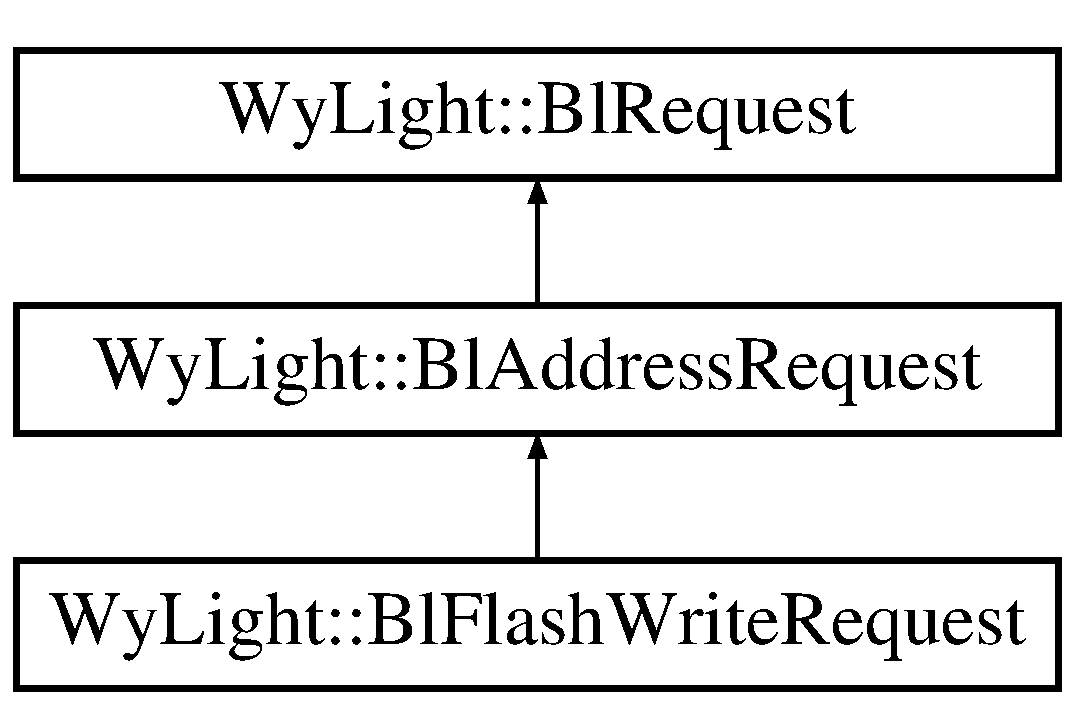
\includegraphics[height=3.000000cm]{struct_wy_light_1_1_bl_flash_write_request}
\end{center}
\end{figure}
\subsection*{Public Member Functions}
\begin{DoxyCompactItemize}
\item 
\hyperlink{struct_wy_light_1_1_bl_flash_write_request_a00cecca6b19636cd189ee778ed5a7c41}{Bl\-Flash\-Write\-Request} ()
\item 
void \hyperlink{struct_wy_light_1_1_bl_flash_write_request_a7ad0fd6001817041996e9014d12e3334}{Set\-Data} (unsigned int address, unsigned char $\ast$p\-Data, size\-\_\-t num\-Bytes)
\end{DoxyCompactItemize}
\subsection*{Public Attributes}
\begin{DoxyCompactItemize}
\item 
unsigned char \hyperlink{struct_wy_light_1_1_bl_flash_write_request_a5a505e0a8efd8266cf248251a6f16d95}{num\-Blocks\-Low}
\item 
unsigned char \hyperlink{struct_wy_light_1_1_bl_flash_write_request_a79a8eab1d1d25b3acd1639e31c70539f}{payload} \mbox{[}\hyperlink{_bl_request_8h_ae93d0b04d7bc152e72713dc07fcc1e9f}{F\-L\-A\-S\-H\-\_\-\-W\-R\-I\-T\-E\-\_\-\-B\-L\-O\-C\-K\-S\-I\-Z\-E}\mbox{]}
\end{DoxyCompactItemize}


\subsection{Constructor \& Destructor Documentation}
\hypertarget{struct_wy_light_1_1_bl_flash_write_request_a00cecca6b19636cd189ee778ed5a7c41}{\index{Wy\-Light\-::\-Bl\-Flash\-Write\-Request@{Wy\-Light\-::\-Bl\-Flash\-Write\-Request}!Bl\-Flash\-Write\-Request@{Bl\-Flash\-Write\-Request}}
\index{Bl\-Flash\-Write\-Request@{Bl\-Flash\-Write\-Request}!WyLight::BlFlashWriteRequest@{Wy\-Light\-::\-Bl\-Flash\-Write\-Request}}
\subsubsection[{Bl\-Flash\-Write\-Request}]{\setlength{\rightskip}{0pt plus 5cm}Wy\-Light\-::\-Bl\-Flash\-Write\-Request\-::\-Bl\-Flash\-Write\-Request (
\begin{DoxyParamCaption}
{}
\end{DoxyParamCaption}
)\hspace{0.3cm}{\ttfamily [inline]}}}\label{struct_wy_light_1_1_bl_flash_write_request_a00cecca6b19636cd189ee778ed5a7c41}


\subsection{Member Function Documentation}
\hypertarget{struct_wy_light_1_1_bl_flash_write_request_a7ad0fd6001817041996e9014d12e3334}{\index{Wy\-Light\-::\-Bl\-Flash\-Write\-Request@{Wy\-Light\-::\-Bl\-Flash\-Write\-Request}!Set\-Data@{Set\-Data}}
\index{Set\-Data@{Set\-Data}!WyLight::BlFlashWriteRequest@{Wy\-Light\-::\-Bl\-Flash\-Write\-Request}}
\subsubsection[{Set\-Data}]{\setlength{\rightskip}{0pt plus 5cm}void Wy\-Light\-::\-Bl\-Flash\-Write\-Request\-::\-Set\-Data (
\begin{DoxyParamCaption}
\item[{unsigned int}]{address, }
\item[{unsigned char $\ast$}]{p\-Data, }
\item[{size\-\_\-t}]{num\-Bytes}
\end{DoxyParamCaption}
)\hspace{0.3cm}{\ttfamily [inline]}}}\label{struct_wy_light_1_1_bl_flash_write_request_a7ad0fd6001817041996e9014d12e3334}


\subsection{Member Data Documentation}
\hypertarget{struct_wy_light_1_1_bl_flash_write_request_a5a505e0a8efd8266cf248251a6f16d95}{\index{Wy\-Light\-::\-Bl\-Flash\-Write\-Request@{Wy\-Light\-::\-Bl\-Flash\-Write\-Request}!num\-Blocks\-Low@{num\-Blocks\-Low}}
\index{num\-Blocks\-Low@{num\-Blocks\-Low}!WyLight::BlFlashWriteRequest@{Wy\-Light\-::\-Bl\-Flash\-Write\-Request}}
\subsubsection[{num\-Blocks\-Low}]{\setlength{\rightskip}{0pt plus 5cm}unsigned char Wy\-Light\-::\-Bl\-Flash\-Write\-Request\-::num\-Blocks\-Low}}\label{struct_wy_light_1_1_bl_flash_write_request_a5a505e0a8efd8266cf248251a6f16d95}
\hypertarget{struct_wy_light_1_1_bl_flash_write_request_a79a8eab1d1d25b3acd1639e31c70539f}{\index{Wy\-Light\-::\-Bl\-Flash\-Write\-Request@{Wy\-Light\-::\-Bl\-Flash\-Write\-Request}!payload@{payload}}
\index{payload@{payload}!WyLight::BlFlashWriteRequest@{Wy\-Light\-::\-Bl\-Flash\-Write\-Request}}
\subsubsection[{payload}]{\setlength{\rightskip}{0pt plus 5cm}unsigned char Wy\-Light\-::\-Bl\-Flash\-Write\-Request\-::payload\mbox{[}{\bf F\-L\-A\-S\-H\-\_\-\-W\-R\-I\-T\-E\-\_\-\-B\-L\-O\-C\-K\-S\-I\-Z\-E}\mbox{]}}}\label{struct_wy_light_1_1_bl_flash_write_request_a79a8eab1d1d25b3acd1639e31c70539f}


The documentation for this struct was generated from the following file\-:\begin{DoxyCompactItemize}
\item 
library/\hyperlink{_bl_request_8h}{Bl\-Request.\-h}\end{DoxyCompactItemize}

\hypertarget{struct_wy_light_1_1_bl_info}{\section{Wy\-Light\-:\-:Bl\-Info Struct Reference}
\label{struct_wy_light_1_1_bl_info}\index{Wy\-Light\-::\-Bl\-Info@{Wy\-Light\-::\-Bl\-Info}}
}


{\ttfamily \#include $<$Bl\-Request.\-h$>$}

\subsection*{Public Member Functions}
\begin{DoxyCompactItemize}
\item 
uint32\-\_\-t \hyperlink{struct_wy_light_1_1_bl_info_a93505c5f081c862b51e1f0dc746b6f0a}{Get\-Address} (void) const 
\item 
void \hyperlink{struct_wy_light_1_1_bl_info_a8567ca010c4dfac79426c44eeca2369a}{Print} (void) const 
\end{DoxyCompactItemize}
\subsection*{Public Attributes}
\begin{DoxyCompactItemize}
\item 
unsigned char \hyperlink{struct_wy_light_1_1_bl_info_a0fdc843fbc878f3570751ef38fa69e0e}{size\-Low}
\item 
unsigned char \hyperlink{struct_wy_light_1_1_bl_info_a95dfd12b33d938d0130d1e3326f9d711}{size\-High}
\item 
unsigned char \hyperlink{struct_wy_light_1_1_bl_info_a225c43b9cc621dd383ca22695098f2a6}{version\-Major}
\item 
unsigned char \hyperlink{struct_wy_light_1_1_bl_info_a416fdd8a8cd832aca5f6f6ae851d91ff}{version\-Minor}
\item 
unsigned char \hyperlink{struct_wy_light_1_1_bl_info_a6dfdd03e93374830817109e096103b69}{cmdmask\-High}
\item 
unsigned char \hyperlink{struct_wy_light_1_1_bl_info_a716367b951d25272fc9f95324e10fa73}{family\-Id}\-: 4
\item 
unsigned char \hyperlink{struct_wy_light_1_1_bl_info_a7ebeda2077accbc4de2305114efb6f4b}{cmdmask\-Low}\-:4
\item 
unsigned char \hyperlink{struct_wy_light_1_1_bl_info_a7a53fd44ef6def50cbffdc519190961d}{start\-Low}
\item 
unsigned char \hyperlink{struct_wy_light_1_1_bl_info_adaaa62eb1ad8fee73cb2503222e7b905}{start\-High}
\item 
unsigned char \hyperlink{struct_wy_light_1_1_bl_info_a9d435ba3c8d9b530b3fcbf70c358e72c}{start\-U}
\item 
unsigned char \hyperlink{struct_wy_light_1_1_bl_info_a824d4777a879a587bee8c68461226883}{zero}
\end{DoxyCompactItemize}


\subsection{Member Function Documentation}
\hypertarget{struct_wy_light_1_1_bl_info_a93505c5f081c862b51e1f0dc746b6f0a}{\index{Wy\-Light\-::\-Bl\-Info@{Wy\-Light\-::\-Bl\-Info}!Get\-Address@{Get\-Address}}
\index{Get\-Address@{Get\-Address}!WyLight::BlInfo@{Wy\-Light\-::\-Bl\-Info}}
\subsubsection[{Get\-Address}]{\setlength{\rightskip}{0pt plus 5cm}uint32\-\_\-t Wy\-Light\-::\-Bl\-Info\-::\-Get\-Address (
\begin{DoxyParamCaption}
\item[{void}]{}
\end{DoxyParamCaption}
) const\hspace{0.3cm}{\ttfamily [inline]}}}\label{struct_wy_light_1_1_bl_info_a93505c5f081c862b51e1f0dc746b6f0a}
\hypertarget{struct_wy_light_1_1_bl_info_a8567ca010c4dfac79426c44eeca2369a}{\index{Wy\-Light\-::\-Bl\-Info@{Wy\-Light\-::\-Bl\-Info}!Print@{Print}}
\index{Print@{Print}!WyLight::BlInfo@{Wy\-Light\-::\-Bl\-Info}}
\subsubsection[{Print}]{\setlength{\rightskip}{0pt plus 5cm}void Wy\-Light\-::\-Bl\-Info\-::\-Print (
\begin{DoxyParamCaption}
\item[{void}]{}
\end{DoxyParamCaption}
) const\hspace{0.3cm}{\ttfamily [inline]}}}\label{struct_wy_light_1_1_bl_info_a8567ca010c4dfac79426c44eeca2369a}


\subsection{Member Data Documentation}
\hypertarget{struct_wy_light_1_1_bl_info_a6dfdd03e93374830817109e096103b69}{\index{Wy\-Light\-::\-Bl\-Info@{Wy\-Light\-::\-Bl\-Info}!cmdmask\-High@{cmdmask\-High}}
\index{cmdmask\-High@{cmdmask\-High}!WyLight::BlInfo@{Wy\-Light\-::\-Bl\-Info}}
\subsubsection[{cmdmask\-High}]{\setlength{\rightskip}{0pt plus 5cm}unsigned char Wy\-Light\-::\-Bl\-Info\-::cmdmask\-High}}\label{struct_wy_light_1_1_bl_info_a6dfdd03e93374830817109e096103b69}
\hypertarget{struct_wy_light_1_1_bl_info_a7ebeda2077accbc4de2305114efb6f4b}{\index{Wy\-Light\-::\-Bl\-Info@{Wy\-Light\-::\-Bl\-Info}!cmdmask\-Low@{cmdmask\-Low}}
\index{cmdmask\-Low@{cmdmask\-Low}!WyLight::BlInfo@{Wy\-Light\-::\-Bl\-Info}}
\subsubsection[{cmdmask\-Low}]{\setlength{\rightskip}{0pt plus 5cm}unsigned char Wy\-Light\-::\-Bl\-Info\-::cmdmask\-Low}}\label{struct_wy_light_1_1_bl_info_a7ebeda2077accbc4de2305114efb6f4b}
\hypertarget{struct_wy_light_1_1_bl_info_a716367b951d25272fc9f95324e10fa73}{\index{Wy\-Light\-::\-Bl\-Info@{Wy\-Light\-::\-Bl\-Info}!family\-Id@{family\-Id}}
\index{family\-Id@{family\-Id}!WyLight::BlInfo@{Wy\-Light\-::\-Bl\-Info}}
\subsubsection[{family\-Id}]{\setlength{\rightskip}{0pt plus 5cm}unsigned char Wy\-Light\-::\-Bl\-Info\-::family\-Id}}\label{struct_wy_light_1_1_bl_info_a716367b951d25272fc9f95324e10fa73}
\hypertarget{struct_wy_light_1_1_bl_info_a95dfd12b33d938d0130d1e3326f9d711}{\index{Wy\-Light\-::\-Bl\-Info@{Wy\-Light\-::\-Bl\-Info}!size\-High@{size\-High}}
\index{size\-High@{size\-High}!WyLight::BlInfo@{Wy\-Light\-::\-Bl\-Info}}
\subsubsection[{size\-High}]{\setlength{\rightskip}{0pt plus 5cm}unsigned char Wy\-Light\-::\-Bl\-Info\-::size\-High}}\label{struct_wy_light_1_1_bl_info_a95dfd12b33d938d0130d1e3326f9d711}
\hypertarget{struct_wy_light_1_1_bl_info_a0fdc843fbc878f3570751ef38fa69e0e}{\index{Wy\-Light\-::\-Bl\-Info@{Wy\-Light\-::\-Bl\-Info}!size\-Low@{size\-Low}}
\index{size\-Low@{size\-Low}!WyLight::BlInfo@{Wy\-Light\-::\-Bl\-Info}}
\subsubsection[{size\-Low}]{\setlength{\rightskip}{0pt plus 5cm}unsigned char Wy\-Light\-::\-Bl\-Info\-::size\-Low}}\label{struct_wy_light_1_1_bl_info_a0fdc843fbc878f3570751ef38fa69e0e}
\hypertarget{struct_wy_light_1_1_bl_info_adaaa62eb1ad8fee73cb2503222e7b905}{\index{Wy\-Light\-::\-Bl\-Info@{Wy\-Light\-::\-Bl\-Info}!start\-High@{start\-High}}
\index{start\-High@{start\-High}!WyLight::BlInfo@{Wy\-Light\-::\-Bl\-Info}}
\subsubsection[{start\-High}]{\setlength{\rightskip}{0pt plus 5cm}unsigned char Wy\-Light\-::\-Bl\-Info\-::start\-High}}\label{struct_wy_light_1_1_bl_info_adaaa62eb1ad8fee73cb2503222e7b905}
\hypertarget{struct_wy_light_1_1_bl_info_a7a53fd44ef6def50cbffdc519190961d}{\index{Wy\-Light\-::\-Bl\-Info@{Wy\-Light\-::\-Bl\-Info}!start\-Low@{start\-Low}}
\index{start\-Low@{start\-Low}!WyLight::BlInfo@{Wy\-Light\-::\-Bl\-Info}}
\subsubsection[{start\-Low}]{\setlength{\rightskip}{0pt plus 5cm}unsigned char Wy\-Light\-::\-Bl\-Info\-::start\-Low}}\label{struct_wy_light_1_1_bl_info_a7a53fd44ef6def50cbffdc519190961d}
\hypertarget{struct_wy_light_1_1_bl_info_a9d435ba3c8d9b530b3fcbf70c358e72c}{\index{Wy\-Light\-::\-Bl\-Info@{Wy\-Light\-::\-Bl\-Info}!start\-U@{start\-U}}
\index{start\-U@{start\-U}!WyLight::BlInfo@{Wy\-Light\-::\-Bl\-Info}}
\subsubsection[{start\-U}]{\setlength{\rightskip}{0pt plus 5cm}unsigned char Wy\-Light\-::\-Bl\-Info\-::start\-U}}\label{struct_wy_light_1_1_bl_info_a9d435ba3c8d9b530b3fcbf70c358e72c}
\hypertarget{struct_wy_light_1_1_bl_info_a225c43b9cc621dd383ca22695098f2a6}{\index{Wy\-Light\-::\-Bl\-Info@{Wy\-Light\-::\-Bl\-Info}!version\-Major@{version\-Major}}
\index{version\-Major@{version\-Major}!WyLight::BlInfo@{Wy\-Light\-::\-Bl\-Info}}
\subsubsection[{version\-Major}]{\setlength{\rightskip}{0pt plus 5cm}unsigned char Wy\-Light\-::\-Bl\-Info\-::version\-Major}}\label{struct_wy_light_1_1_bl_info_a225c43b9cc621dd383ca22695098f2a6}
\hypertarget{struct_wy_light_1_1_bl_info_a416fdd8a8cd832aca5f6f6ae851d91ff}{\index{Wy\-Light\-::\-Bl\-Info@{Wy\-Light\-::\-Bl\-Info}!version\-Minor@{version\-Minor}}
\index{version\-Minor@{version\-Minor}!WyLight::BlInfo@{Wy\-Light\-::\-Bl\-Info}}
\subsubsection[{version\-Minor}]{\setlength{\rightskip}{0pt plus 5cm}unsigned char Wy\-Light\-::\-Bl\-Info\-::version\-Minor}}\label{struct_wy_light_1_1_bl_info_a416fdd8a8cd832aca5f6f6ae851d91ff}
\hypertarget{struct_wy_light_1_1_bl_info_a824d4777a879a587bee8c68461226883}{\index{Wy\-Light\-::\-Bl\-Info@{Wy\-Light\-::\-Bl\-Info}!zero@{zero}}
\index{zero@{zero}!WyLight::BlInfo@{Wy\-Light\-::\-Bl\-Info}}
\subsubsection[{zero}]{\setlength{\rightskip}{0pt plus 5cm}unsigned char Wy\-Light\-::\-Bl\-Info\-::zero}}\label{struct_wy_light_1_1_bl_info_a824d4777a879a587bee8c68461226883}


The documentation for this struct was generated from the following file\-:\begin{DoxyCompactItemize}
\item 
library/\hyperlink{_bl_request_8h}{Bl\-Request.\-h}\end{DoxyCompactItemize}

\hypertarget{struct_wy_light_1_1_bl_info_request}{\section{Wy\-Light\-:\-:Bl\-Info\-Request Struct Reference}
\label{struct_wy_light_1_1_bl_info_request}\index{Wy\-Light\-::\-Bl\-Info\-Request@{Wy\-Light\-::\-Bl\-Info\-Request}}
}


{\ttfamily \#include $<$Bl\-Request.\-h$>$}

Inheritance diagram for Wy\-Light\-:\-:Bl\-Info\-Request\-:\begin{figure}[H]
\begin{center}
\leavevmode
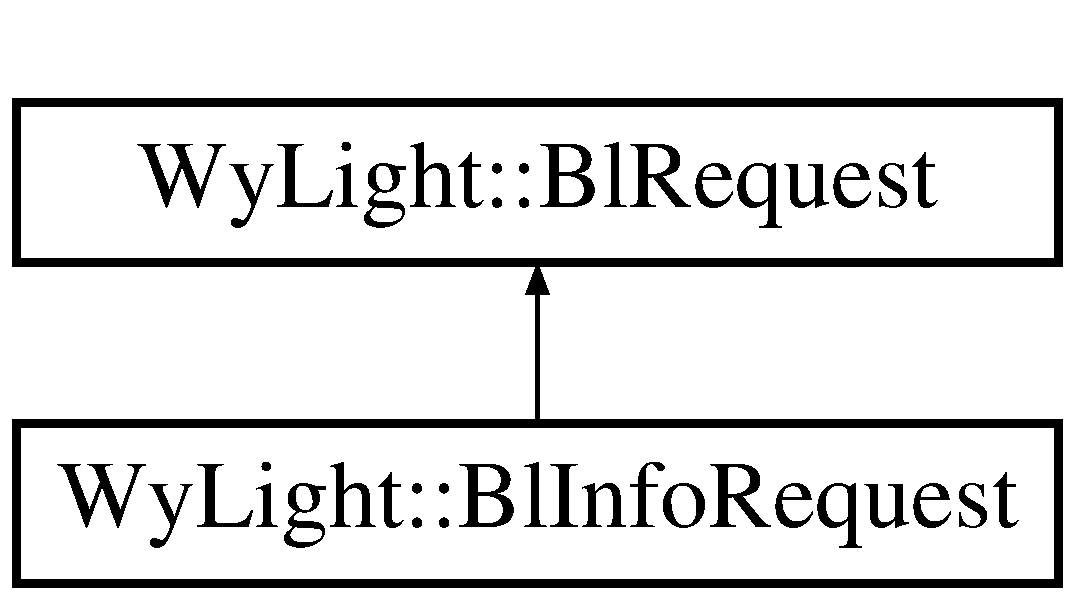
\includegraphics[height=2.000000cm]{struct_wy_light_1_1_bl_info_request}
\end{center}
\end{figure}
\subsection*{Public Member Functions}
\begin{DoxyCompactItemize}
\item 
\hyperlink{struct_wy_light_1_1_bl_info_request_ac029d8a854cf7694e44285fb60996fb1}{Bl\-Info\-Request} ()
\end{DoxyCompactItemize}
\subsection*{Additional Inherited Members}


\subsection{Constructor \& Destructor Documentation}
\hypertarget{struct_wy_light_1_1_bl_info_request_ac029d8a854cf7694e44285fb60996fb1}{\index{Wy\-Light\-::\-Bl\-Info\-Request@{Wy\-Light\-::\-Bl\-Info\-Request}!Bl\-Info\-Request@{Bl\-Info\-Request}}
\index{Bl\-Info\-Request@{Bl\-Info\-Request}!WyLight::BlInfoRequest@{Wy\-Light\-::\-Bl\-Info\-Request}}
\subsubsection[{Bl\-Info\-Request}]{\setlength{\rightskip}{0pt plus 5cm}Wy\-Light\-::\-Bl\-Info\-Request\-::\-Bl\-Info\-Request (
\begin{DoxyParamCaption}
{}
\end{DoxyParamCaption}
)\hspace{0.3cm}{\ttfamily [inline]}}}\label{struct_wy_light_1_1_bl_info_request_ac029d8a854cf7694e44285fb60996fb1}


The documentation for this struct was generated from the following file\-:\begin{DoxyCompactItemize}
\item 
library/\hyperlink{_bl_request_8h}{Bl\-Request.\-h}\end{DoxyCompactItemize}

\hypertarget{struct_wy_light_1_1_bl_read_request}{\section{Wy\-Light\-:\-:Bl\-Read\-Request Struct Reference}
\label{struct_wy_light_1_1_bl_read_request}\index{Wy\-Light\-::\-Bl\-Read\-Request@{Wy\-Light\-::\-Bl\-Read\-Request}}
}


{\ttfamily \#include $<$Bl\-Request.\-h$>$}

Inheritance diagram for Wy\-Light\-:\-:Bl\-Read\-Request\-:\begin{figure}[H]
\begin{center}
\leavevmode
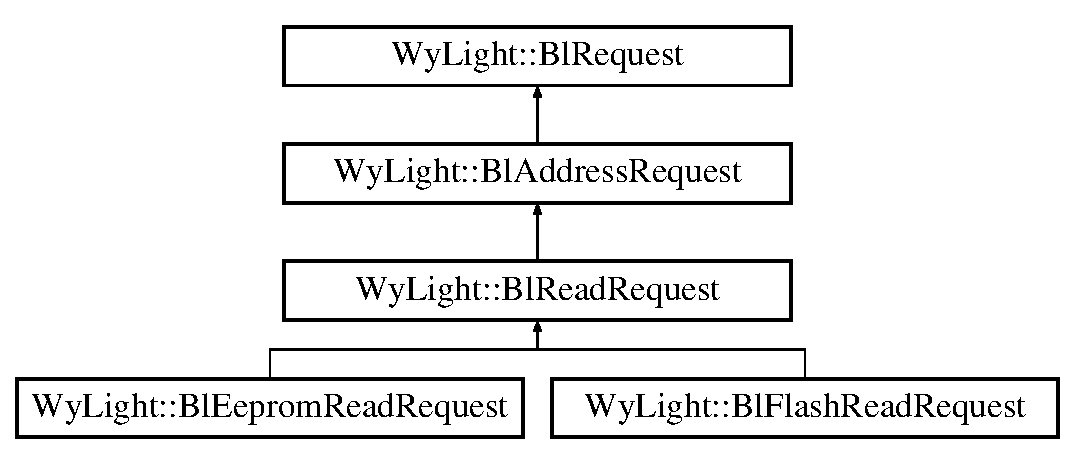
\includegraphics[height=4.000000cm]{struct_wy_light_1_1_bl_read_request}
\end{center}
\end{figure}
\subsection*{Public Member Functions}
\begin{DoxyCompactItemize}
\item 
\hyperlink{struct_wy_light_1_1_bl_read_request_ab9f77571421d6f5cde7e54a3396e0f37}{Bl\-Read\-Request} (size\-\_\-t size, unsigned char cmd)
\item 
void \hyperlink{struct_wy_light_1_1_bl_read_request_a84b7b977397f292a5dee65fcbf4d5c1f}{Set\-Address\-Num\-Bytes} (unsigned int address, unsigned short num\-Bytes)
\end{DoxyCompactItemize}
\subsection*{Public Attributes}
\begin{DoxyCompactItemize}
\item 
unsigned char \hyperlink{struct_wy_light_1_1_bl_read_request_afcf7c581f226c10726999e4aca344137}{num\-Bytes\-Low}
\item 
unsigned char \hyperlink{struct_wy_light_1_1_bl_read_request_abaf19abf5aa4e5e787eae732210b5c81}{num\-Bytes\-High}
\end{DoxyCompactItemize}


\subsection{Constructor \& Destructor Documentation}
\hypertarget{struct_wy_light_1_1_bl_read_request_ab9f77571421d6f5cde7e54a3396e0f37}{\index{Wy\-Light\-::\-Bl\-Read\-Request@{Wy\-Light\-::\-Bl\-Read\-Request}!Bl\-Read\-Request@{Bl\-Read\-Request}}
\index{Bl\-Read\-Request@{Bl\-Read\-Request}!WyLight::BlReadRequest@{Wy\-Light\-::\-Bl\-Read\-Request}}
\subsubsection[{Bl\-Read\-Request}]{\setlength{\rightskip}{0pt plus 5cm}Wy\-Light\-::\-Bl\-Read\-Request\-::\-Bl\-Read\-Request (
\begin{DoxyParamCaption}
\item[{size\-\_\-t}]{size, }
\item[{unsigned char}]{cmd}
\end{DoxyParamCaption}
)\hspace{0.3cm}{\ttfamily [inline]}}}\label{struct_wy_light_1_1_bl_read_request_ab9f77571421d6f5cde7e54a3396e0f37}


\subsection{Member Function Documentation}
\hypertarget{struct_wy_light_1_1_bl_read_request_a84b7b977397f292a5dee65fcbf4d5c1f}{\index{Wy\-Light\-::\-Bl\-Read\-Request@{Wy\-Light\-::\-Bl\-Read\-Request}!Set\-Address\-Num\-Bytes@{Set\-Address\-Num\-Bytes}}
\index{Set\-Address\-Num\-Bytes@{Set\-Address\-Num\-Bytes}!WyLight::BlReadRequest@{Wy\-Light\-::\-Bl\-Read\-Request}}
\subsubsection[{Set\-Address\-Num\-Bytes}]{\setlength{\rightskip}{0pt plus 5cm}void Wy\-Light\-::\-Bl\-Read\-Request\-::\-Set\-Address\-Num\-Bytes (
\begin{DoxyParamCaption}
\item[{unsigned int}]{address, }
\item[{unsigned short}]{num\-Bytes}
\end{DoxyParamCaption}
)\hspace{0.3cm}{\ttfamily [inline]}}}\label{struct_wy_light_1_1_bl_read_request_a84b7b977397f292a5dee65fcbf4d5c1f}


\subsection{Member Data Documentation}
\hypertarget{struct_wy_light_1_1_bl_read_request_abaf19abf5aa4e5e787eae732210b5c81}{\index{Wy\-Light\-::\-Bl\-Read\-Request@{Wy\-Light\-::\-Bl\-Read\-Request}!num\-Bytes\-High@{num\-Bytes\-High}}
\index{num\-Bytes\-High@{num\-Bytes\-High}!WyLight::BlReadRequest@{Wy\-Light\-::\-Bl\-Read\-Request}}
\subsubsection[{num\-Bytes\-High}]{\setlength{\rightskip}{0pt plus 5cm}unsigned char Wy\-Light\-::\-Bl\-Read\-Request\-::num\-Bytes\-High}}\label{struct_wy_light_1_1_bl_read_request_abaf19abf5aa4e5e787eae732210b5c81}
\hypertarget{struct_wy_light_1_1_bl_read_request_afcf7c581f226c10726999e4aca344137}{\index{Wy\-Light\-::\-Bl\-Read\-Request@{Wy\-Light\-::\-Bl\-Read\-Request}!num\-Bytes\-Low@{num\-Bytes\-Low}}
\index{num\-Bytes\-Low@{num\-Bytes\-Low}!WyLight::BlReadRequest@{Wy\-Light\-::\-Bl\-Read\-Request}}
\subsubsection[{num\-Bytes\-Low}]{\setlength{\rightskip}{0pt plus 5cm}unsigned char Wy\-Light\-::\-Bl\-Read\-Request\-::num\-Bytes\-Low}}\label{struct_wy_light_1_1_bl_read_request_afcf7c581f226c10726999e4aca344137}


The documentation for this struct was generated from the following file\-:\begin{DoxyCompactItemize}
\item 
library/\hyperlink{_bl_request_8h}{Bl\-Request.\-h}\end{DoxyCompactItemize}

\hypertarget{struct_wy_light_1_1_bl_request}{\section{Wy\-Light\-:\-:Bl\-Request Struct Reference}
\label{struct_wy_light_1_1_bl_request}\index{Wy\-Light\-::\-Bl\-Request@{Wy\-Light\-::\-Bl\-Request}}
}


{\ttfamily \#include $<$Bl\-Request.\-h$>$}

Inheritance diagram for Wy\-Light\-:\-:Bl\-Request\-:\begin{figure}[H]
\begin{center}
\leavevmode
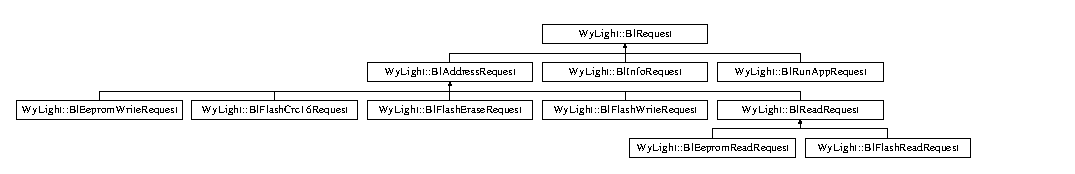
\includegraphics[height=1.885522cm]{struct_wy_light_1_1_bl_request}
\end{center}
\end{figure}
\subsection*{Public Member Functions}
\begin{DoxyCompactItemize}
\item 
\hyperlink{struct_wy_light_1_1_bl_request_a4a851665f3b0c945c63023f0d30f909c}{Bl\-Request} (size\-\_\-t size, unsigned char cmd)
\item 
const unsigned char $\ast$ \hyperlink{struct_wy_light_1_1_bl_request_a0d956ad98677f0d309c031d00d797f90}{Get\-Data} () const 
\item 
size\-\_\-t \hyperlink{struct_wy_light_1_1_bl_request_a46864fa4524fcdd0f32033e8f51ba1c5}{Get\-Size} () const 
\item 
virtual bool \hyperlink{struct_wy_light_1_1_bl_request_a35e6aeaab96cce48c4dcc2f63eb920c4}{Check\-Crc} () const 
\end{DoxyCompactItemize}
\subsection*{Public Attributes}
\begin{DoxyCompactItemize}
\item 
const size\-\_\-t \hyperlink{struct_wy_light_1_1_bl_request_afa34d5447875f08e32d1a8b1de10685f}{m\-Size}
\item 
const unsigned char \hyperlink{struct_wy_light_1_1_bl_request_a8d9f248e23c6e940bf6c23f9bdbcbb37}{m\-Cmd}
\end{DoxyCompactItemize}


\subsection{Constructor \& Destructor Documentation}
\hypertarget{struct_wy_light_1_1_bl_request_a4a851665f3b0c945c63023f0d30f909c}{\index{Wy\-Light\-::\-Bl\-Request@{Wy\-Light\-::\-Bl\-Request}!Bl\-Request@{Bl\-Request}}
\index{Bl\-Request@{Bl\-Request}!WyLight::BlRequest@{Wy\-Light\-::\-Bl\-Request}}
\subsubsection[{Bl\-Request}]{\setlength{\rightskip}{0pt plus 5cm}Wy\-Light\-::\-Bl\-Request\-::\-Bl\-Request (
\begin{DoxyParamCaption}
\item[{size\-\_\-t}]{size, }
\item[{unsigned char}]{cmd}
\end{DoxyParamCaption}
)\hspace{0.3cm}{\ttfamily [inline]}}}\label{struct_wy_light_1_1_bl_request_a4a851665f3b0c945c63023f0d30f909c}


\subsection{Member Function Documentation}
\hypertarget{struct_wy_light_1_1_bl_request_a35e6aeaab96cce48c4dcc2f63eb920c4}{\index{Wy\-Light\-::\-Bl\-Request@{Wy\-Light\-::\-Bl\-Request}!Check\-Crc@{Check\-Crc}}
\index{Check\-Crc@{Check\-Crc}!WyLight::BlRequest@{Wy\-Light\-::\-Bl\-Request}}
\subsubsection[{Check\-Crc}]{\setlength{\rightskip}{0pt plus 5cm}virtual bool Wy\-Light\-::\-Bl\-Request\-::\-Check\-Crc (
\begin{DoxyParamCaption}
{}
\end{DoxyParamCaption}
) const\hspace{0.3cm}{\ttfamily [inline]}, {\ttfamily [virtual]}}}\label{struct_wy_light_1_1_bl_request_a35e6aeaab96cce48c4dcc2f63eb920c4}


Reimplemented in \hyperlink{struct_wy_light_1_1_bl_run_app_request_a2d59de738e6f5303dd6e0b8a842f33b8}{Wy\-Light\-::\-Bl\-Run\-App\-Request}, and \hyperlink{struct_wy_light_1_1_bl_flash_crc16_request_a7a3a14722ed86688b5992f84089adc3c}{Wy\-Light\-::\-Bl\-Flash\-Crc16\-Request}.

\hypertarget{struct_wy_light_1_1_bl_request_a0d956ad98677f0d309c031d00d797f90}{\index{Wy\-Light\-::\-Bl\-Request@{Wy\-Light\-::\-Bl\-Request}!Get\-Data@{Get\-Data}}
\index{Get\-Data@{Get\-Data}!WyLight::BlRequest@{Wy\-Light\-::\-Bl\-Request}}
\subsubsection[{Get\-Data}]{\setlength{\rightskip}{0pt plus 5cm}const unsigned char$\ast$ Wy\-Light\-::\-Bl\-Request\-::\-Get\-Data (
\begin{DoxyParamCaption}
{}
\end{DoxyParamCaption}
) const\hspace{0.3cm}{\ttfamily [inline]}}}\label{struct_wy_light_1_1_bl_request_a0d956ad98677f0d309c031d00d797f90}
\hypertarget{struct_wy_light_1_1_bl_request_a46864fa4524fcdd0f32033e8f51ba1c5}{\index{Wy\-Light\-::\-Bl\-Request@{Wy\-Light\-::\-Bl\-Request}!Get\-Size@{Get\-Size}}
\index{Get\-Size@{Get\-Size}!WyLight::BlRequest@{Wy\-Light\-::\-Bl\-Request}}
\subsubsection[{Get\-Size}]{\setlength{\rightskip}{0pt plus 5cm}size\-\_\-t Wy\-Light\-::\-Bl\-Request\-::\-Get\-Size (
\begin{DoxyParamCaption}
{}
\end{DoxyParamCaption}
) const\hspace{0.3cm}{\ttfamily [inline]}}}\label{struct_wy_light_1_1_bl_request_a46864fa4524fcdd0f32033e8f51ba1c5}


\subsection{Member Data Documentation}
\hypertarget{struct_wy_light_1_1_bl_request_a8d9f248e23c6e940bf6c23f9bdbcbb37}{\index{Wy\-Light\-::\-Bl\-Request@{Wy\-Light\-::\-Bl\-Request}!m\-Cmd@{m\-Cmd}}
\index{m\-Cmd@{m\-Cmd}!WyLight::BlRequest@{Wy\-Light\-::\-Bl\-Request}}
\subsubsection[{m\-Cmd}]{\setlength{\rightskip}{0pt plus 5cm}const unsigned char Wy\-Light\-::\-Bl\-Request\-::m\-Cmd}}\label{struct_wy_light_1_1_bl_request_a8d9f248e23c6e940bf6c23f9bdbcbb37}
\hypertarget{struct_wy_light_1_1_bl_request_afa34d5447875f08e32d1a8b1de10685f}{\index{Wy\-Light\-::\-Bl\-Request@{Wy\-Light\-::\-Bl\-Request}!m\-Size@{m\-Size}}
\index{m\-Size@{m\-Size}!WyLight::BlRequest@{Wy\-Light\-::\-Bl\-Request}}
\subsubsection[{m\-Size}]{\setlength{\rightskip}{0pt plus 5cm}const size\-\_\-t Wy\-Light\-::\-Bl\-Request\-::m\-Size}}\label{struct_wy_light_1_1_bl_request_afa34d5447875f08e32d1a8b1de10685f}


The documentation for this struct was generated from the following file\-:\begin{DoxyCompactItemize}
\item 
library/\hyperlink{_bl_request_8h}{Bl\-Request.\-h}\end{DoxyCompactItemize}

\hypertarget{struct_wy_light_1_1_bl_run_app_request}{\section{Wy\-Light\-:\-:Bl\-Run\-App\-Request Struct Reference}
\label{struct_wy_light_1_1_bl_run_app_request}\index{Wy\-Light\-::\-Bl\-Run\-App\-Request@{Wy\-Light\-::\-Bl\-Run\-App\-Request}}
}


{\ttfamily \#include $<$Bl\-Request.\-h$>$}

Inheritance diagram for Wy\-Light\-:\-:Bl\-Run\-App\-Request\-:\begin{figure}[H]
\begin{center}
\leavevmode
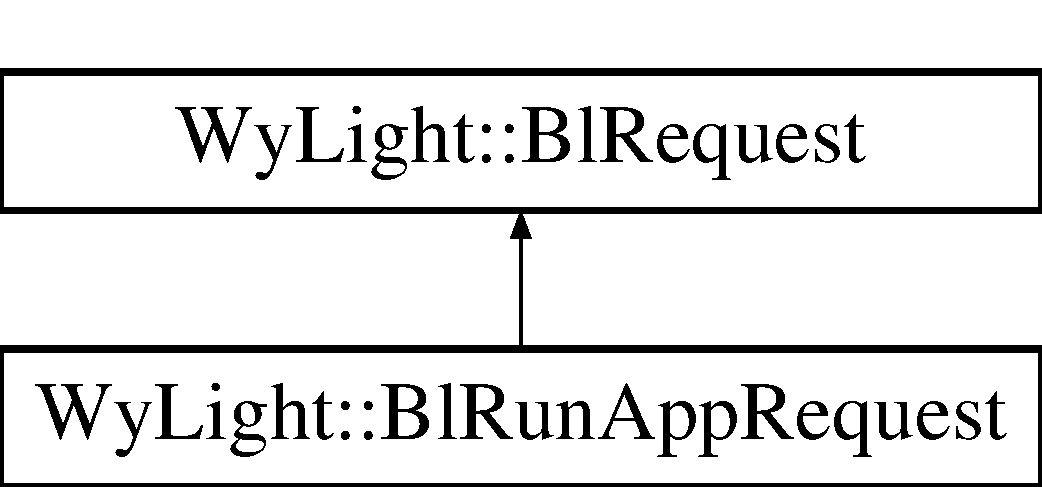
\includegraphics[height=2.000000cm]{struct_wy_light_1_1_bl_run_app_request}
\end{center}
\end{figure}
\subsection*{Public Member Functions}
\begin{DoxyCompactItemize}
\item 
\hyperlink{struct_wy_light_1_1_bl_run_app_request_aa6a3f48d0ee9b9194f2a8af808d6185f}{Bl\-Run\-App\-Request} ()
\item 
virtual bool \hyperlink{struct_wy_light_1_1_bl_run_app_request_a2d59de738e6f5303dd6e0b8a842f33b8}{Check\-Crc} () const 
\end{DoxyCompactItemize}
\subsection*{Additional Inherited Members}


\subsection{Constructor \& Destructor Documentation}
\hypertarget{struct_wy_light_1_1_bl_run_app_request_aa6a3f48d0ee9b9194f2a8af808d6185f}{\index{Wy\-Light\-::\-Bl\-Run\-App\-Request@{Wy\-Light\-::\-Bl\-Run\-App\-Request}!Bl\-Run\-App\-Request@{Bl\-Run\-App\-Request}}
\index{Bl\-Run\-App\-Request@{Bl\-Run\-App\-Request}!WyLight::BlRunAppRequest@{Wy\-Light\-::\-Bl\-Run\-App\-Request}}
\subsubsection[{Bl\-Run\-App\-Request}]{\setlength{\rightskip}{0pt plus 5cm}Wy\-Light\-::\-Bl\-Run\-App\-Request\-::\-Bl\-Run\-App\-Request (
\begin{DoxyParamCaption}
{}
\end{DoxyParamCaption}
)\hspace{0.3cm}{\ttfamily [inline]}}}\label{struct_wy_light_1_1_bl_run_app_request_aa6a3f48d0ee9b9194f2a8af808d6185f}


\subsection{Member Function Documentation}
\hypertarget{struct_wy_light_1_1_bl_run_app_request_a2d59de738e6f5303dd6e0b8a842f33b8}{\index{Wy\-Light\-::\-Bl\-Run\-App\-Request@{Wy\-Light\-::\-Bl\-Run\-App\-Request}!Check\-Crc@{Check\-Crc}}
\index{Check\-Crc@{Check\-Crc}!WyLight::BlRunAppRequest@{Wy\-Light\-::\-Bl\-Run\-App\-Request}}
\subsubsection[{Check\-Crc}]{\setlength{\rightskip}{0pt plus 5cm}virtual bool Wy\-Light\-::\-Bl\-Run\-App\-Request\-::\-Check\-Crc (
\begin{DoxyParamCaption}
{}
\end{DoxyParamCaption}
) const\hspace{0.3cm}{\ttfamily [inline]}, {\ttfamily [virtual]}}}\label{struct_wy_light_1_1_bl_run_app_request_a2d59de738e6f5303dd6e0b8a842f33b8}


Reimplemented from \hyperlink{struct_wy_light_1_1_bl_request_a35e6aeaab96cce48c4dcc2f63eb920c4}{Wy\-Light\-::\-Bl\-Request}.



The documentation for this struct was generated from the following file\-:\begin{DoxyCompactItemize}
\item 
library/\hyperlink{_bl_request_8h}{Bl\-Request.\-h}\end{DoxyCompactItemize}

\hypertarget{struct_wy_light_1_1_broadcast_message}{\section{Wy\-Light\-:\-:Broadcast\-Message Struct Reference}
\label{struct_wy_light_1_1_broadcast_message}\index{Wy\-Light\-::\-Broadcast\-Message@{Wy\-Light\-::\-Broadcast\-Message}}
}


{\ttfamily \#include $<$Broadcast\-Message.\-h$>$}

\subsection*{Public Member Functions}
\begin{DoxyCompactItemize}
\item 
bool \hyperlink{struct_wy_light_1_1_broadcast_message_a1cddfb2dd5da9655d50d7918944d038b}{Is\-Wifly\-Broadcast} (size\-\_\-t length) const 
\end{DoxyCompactItemize}
\subsection*{Public Attributes}
\begin{DoxyCompactItemize}
\item 
uint8\-\_\-t \hyperlink{struct_wy_light_1_1_broadcast_message_a18f1e421ad5fa744476fdb6fe05592a9}{mac} \mbox{[}6\mbox{]}
\item 
uint8\-\_\-t \hyperlink{struct_wy_light_1_1_broadcast_message_a849c4547cb6f96e94e105bbbd2e17aa0}{channel}
\item 
uint8\-\_\-t \hyperlink{struct_wy_light_1_1_broadcast_message_a7284df9957e3fe4d8cc77d5fd64f6ad0}{rssi}
\item 
uint16\-\_\-t \hyperlink{struct_wy_light_1_1_broadcast_message_a876ea107ee7d7a92d8dc026544ab37ca}{port}
\item 
uint32\-\_\-t \hyperlink{struct_wy_light_1_1_broadcast_message_a4cc5a5b440dc793d0ca62b512fd0ca3c}{rtc}
\item 
uint16\-\_\-t \hyperlink{struct_wy_light_1_1_broadcast_message_aece2abbfade1888f969880e9d4cd2bfa}{bat\-\_\-m\-V}
\item 
uint16\-\_\-t \hyperlink{struct_wy_light_1_1_broadcast_message_a3317f27030e3f644bf4c3f29748d2aa0}{gpio\-Value}
\item 
int8\-\_\-t \hyperlink{struct_wy_light_1_1_broadcast_message_ae1c6e62089826e12d7cacdfc2b349a6a}{ascii\-Time} \mbox{[}13+1\mbox{]}
\item 
int8\-\_\-t \hyperlink{struct_wy_light_1_1_broadcast_message_a0a8793ce043e90aab098589663d2284c}{version} \mbox{[}26+1+1\mbox{]}
\item 
int8\-\_\-t \hyperlink{struct_wy_light_1_1_broadcast_message_ae80dfbcfe5dd61783560861f294e7e90}{device\-Id} \mbox{[}32\mbox{]}
\item 
uint16\-\_\-t \hyperlink{struct_wy_light_1_1_broadcast_message_a52b9e5a034569cf7592cd902c292d577}{boot\-Tmms}
\item 
uint16\-\_\-t \hyperlink{struct_wy_light_1_1_broadcast_message_ac999a8e5814f990c66a07b448d961095}{sensor} \mbox{[}8\mbox{]}
\end{DoxyCompactItemize}


\subsection{Member Function Documentation}
\hypertarget{struct_wy_light_1_1_broadcast_message_a1cddfb2dd5da9655d50d7918944d038b}{\index{Wy\-Light\-::\-Broadcast\-Message@{Wy\-Light\-::\-Broadcast\-Message}!Is\-Wifly\-Broadcast@{Is\-Wifly\-Broadcast}}
\index{Is\-Wifly\-Broadcast@{Is\-Wifly\-Broadcast}!WyLight::BroadcastMessage@{Wy\-Light\-::\-Broadcast\-Message}}
\subsubsection[{Is\-Wifly\-Broadcast}]{\setlength{\rightskip}{0pt plus 5cm}bool Wy\-Light\-::\-Broadcast\-Message\-::\-Is\-Wifly\-Broadcast (
\begin{DoxyParamCaption}
\item[{size\-\_\-t}]{length}
\end{DoxyParamCaption}
) const\hspace{0.3cm}{\ttfamily [inline]}}}\label{struct_wy_light_1_1_broadcast_message_a1cddfb2dd5da9655d50d7918944d038b}


\subsection{Member Data Documentation}
\hypertarget{struct_wy_light_1_1_broadcast_message_ae1c6e62089826e12d7cacdfc2b349a6a}{\index{Wy\-Light\-::\-Broadcast\-Message@{Wy\-Light\-::\-Broadcast\-Message}!ascii\-Time@{ascii\-Time}}
\index{ascii\-Time@{ascii\-Time}!WyLight::BroadcastMessage@{Wy\-Light\-::\-Broadcast\-Message}}
\subsubsection[{ascii\-Time}]{\setlength{\rightskip}{0pt plus 5cm}int8\-\_\-t Wy\-Light\-::\-Broadcast\-Message\-::ascii\-Time\mbox{[}13+1\mbox{]}}}\label{struct_wy_light_1_1_broadcast_message_ae1c6e62089826e12d7cacdfc2b349a6a}
\hypertarget{struct_wy_light_1_1_broadcast_message_aece2abbfade1888f969880e9d4cd2bfa}{\index{Wy\-Light\-::\-Broadcast\-Message@{Wy\-Light\-::\-Broadcast\-Message}!bat\-\_\-m\-V@{bat\-\_\-m\-V}}
\index{bat\-\_\-m\-V@{bat\-\_\-m\-V}!WyLight::BroadcastMessage@{Wy\-Light\-::\-Broadcast\-Message}}
\subsubsection[{bat\-\_\-m\-V}]{\setlength{\rightskip}{0pt plus 5cm}uint16\-\_\-t Wy\-Light\-::\-Broadcast\-Message\-::bat\-\_\-m\-V}}\label{struct_wy_light_1_1_broadcast_message_aece2abbfade1888f969880e9d4cd2bfa}
\hypertarget{struct_wy_light_1_1_broadcast_message_a52b9e5a034569cf7592cd902c292d577}{\index{Wy\-Light\-::\-Broadcast\-Message@{Wy\-Light\-::\-Broadcast\-Message}!boot\-Tmms@{boot\-Tmms}}
\index{boot\-Tmms@{boot\-Tmms}!WyLight::BroadcastMessage@{Wy\-Light\-::\-Broadcast\-Message}}
\subsubsection[{boot\-Tmms}]{\setlength{\rightskip}{0pt plus 5cm}uint16\-\_\-t Wy\-Light\-::\-Broadcast\-Message\-::boot\-Tmms}}\label{struct_wy_light_1_1_broadcast_message_a52b9e5a034569cf7592cd902c292d577}
\hypertarget{struct_wy_light_1_1_broadcast_message_a849c4547cb6f96e94e105bbbd2e17aa0}{\index{Wy\-Light\-::\-Broadcast\-Message@{Wy\-Light\-::\-Broadcast\-Message}!channel@{channel}}
\index{channel@{channel}!WyLight::BroadcastMessage@{Wy\-Light\-::\-Broadcast\-Message}}
\subsubsection[{channel}]{\setlength{\rightskip}{0pt plus 5cm}uint8\-\_\-t Wy\-Light\-::\-Broadcast\-Message\-::channel}}\label{struct_wy_light_1_1_broadcast_message_a849c4547cb6f96e94e105bbbd2e17aa0}
\hypertarget{struct_wy_light_1_1_broadcast_message_ae80dfbcfe5dd61783560861f294e7e90}{\index{Wy\-Light\-::\-Broadcast\-Message@{Wy\-Light\-::\-Broadcast\-Message}!device\-Id@{device\-Id}}
\index{device\-Id@{device\-Id}!WyLight::BroadcastMessage@{Wy\-Light\-::\-Broadcast\-Message}}
\subsubsection[{device\-Id}]{\setlength{\rightskip}{0pt plus 5cm}int8\-\_\-t Wy\-Light\-::\-Broadcast\-Message\-::device\-Id\mbox{[}32\mbox{]}}}\label{struct_wy_light_1_1_broadcast_message_ae80dfbcfe5dd61783560861f294e7e90}
\hypertarget{struct_wy_light_1_1_broadcast_message_a3317f27030e3f644bf4c3f29748d2aa0}{\index{Wy\-Light\-::\-Broadcast\-Message@{Wy\-Light\-::\-Broadcast\-Message}!gpio\-Value@{gpio\-Value}}
\index{gpio\-Value@{gpio\-Value}!WyLight::BroadcastMessage@{Wy\-Light\-::\-Broadcast\-Message}}
\subsubsection[{gpio\-Value}]{\setlength{\rightskip}{0pt plus 5cm}uint16\-\_\-t Wy\-Light\-::\-Broadcast\-Message\-::gpio\-Value}}\label{struct_wy_light_1_1_broadcast_message_a3317f27030e3f644bf4c3f29748d2aa0}
\hypertarget{struct_wy_light_1_1_broadcast_message_a18f1e421ad5fa744476fdb6fe05592a9}{\index{Wy\-Light\-::\-Broadcast\-Message@{Wy\-Light\-::\-Broadcast\-Message}!mac@{mac}}
\index{mac@{mac}!WyLight::BroadcastMessage@{Wy\-Light\-::\-Broadcast\-Message}}
\subsubsection[{mac}]{\setlength{\rightskip}{0pt plus 5cm}uint8\-\_\-t Wy\-Light\-::\-Broadcast\-Message\-::mac\mbox{[}6\mbox{]}}}\label{struct_wy_light_1_1_broadcast_message_a18f1e421ad5fa744476fdb6fe05592a9}
\hypertarget{struct_wy_light_1_1_broadcast_message_a876ea107ee7d7a92d8dc026544ab37ca}{\index{Wy\-Light\-::\-Broadcast\-Message@{Wy\-Light\-::\-Broadcast\-Message}!port@{port}}
\index{port@{port}!WyLight::BroadcastMessage@{Wy\-Light\-::\-Broadcast\-Message}}
\subsubsection[{port}]{\setlength{\rightskip}{0pt plus 5cm}uint16\-\_\-t Wy\-Light\-::\-Broadcast\-Message\-::port}}\label{struct_wy_light_1_1_broadcast_message_a876ea107ee7d7a92d8dc026544ab37ca}
\hypertarget{struct_wy_light_1_1_broadcast_message_a7284df9957e3fe4d8cc77d5fd64f6ad0}{\index{Wy\-Light\-::\-Broadcast\-Message@{Wy\-Light\-::\-Broadcast\-Message}!rssi@{rssi}}
\index{rssi@{rssi}!WyLight::BroadcastMessage@{Wy\-Light\-::\-Broadcast\-Message}}
\subsubsection[{rssi}]{\setlength{\rightskip}{0pt plus 5cm}uint8\-\_\-t Wy\-Light\-::\-Broadcast\-Message\-::rssi}}\label{struct_wy_light_1_1_broadcast_message_a7284df9957e3fe4d8cc77d5fd64f6ad0}
\hypertarget{struct_wy_light_1_1_broadcast_message_a4cc5a5b440dc793d0ca62b512fd0ca3c}{\index{Wy\-Light\-::\-Broadcast\-Message@{Wy\-Light\-::\-Broadcast\-Message}!rtc@{rtc}}
\index{rtc@{rtc}!WyLight::BroadcastMessage@{Wy\-Light\-::\-Broadcast\-Message}}
\subsubsection[{rtc}]{\setlength{\rightskip}{0pt plus 5cm}uint32\-\_\-t Wy\-Light\-::\-Broadcast\-Message\-::rtc}}\label{struct_wy_light_1_1_broadcast_message_a4cc5a5b440dc793d0ca62b512fd0ca3c}
\hypertarget{struct_wy_light_1_1_broadcast_message_ac999a8e5814f990c66a07b448d961095}{\index{Wy\-Light\-::\-Broadcast\-Message@{Wy\-Light\-::\-Broadcast\-Message}!sensor@{sensor}}
\index{sensor@{sensor}!WyLight::BroadcastMessage@{Wy\-Light\-::\-Broadcast\-Message}}
\subsubsection[{sensor}]{\setlength{\rightskip}{0pt plus 5cm}uint16\-\_\-t Wy\-Light\-::\-Broadcast\-Message\-::sensor\mbox{[}8\mbox{]}}}\label{struct_wy_light_1_1_broadcast_message_ac999a8e5814f990c66a07b448d961095}
\hypertarget{struct_wy_light_1_1_broadcast_message_a0a8793ce043e90aab098589663d2284c}{\index{Wy\-Light\-::\-Broadcast\-Message@{Wy\-Light\-::\-Broadcast\-Message}!version@{version}}
\index{version@{version}!WyLight::BroadcastMessage@{Wy\-Light\-::\-Broadcast\-Message}}
\subsubsection[{version}]{\setlength{\rightskip}{0pt plus 5cm}int8\-\_\-t Wy\-Light\-::\-Broadcast\-Message\-::version\mbox{[}26+1+1\mbox{]}}}\label{struct_wy_light_1_1_broadcast_message_a0a8793ce043e90aab098589663d2284c}


The documentation for this struct was generated from the following file\-:\begin{DoxyCompactItemize}
\item 
library/\hyperlink{_broadcast_message_8h}{Broadcast\-Message.\-h}\end{DoxyCompactItemize}

\hypertarget{class_wy_light_1_1_broadcast_receiver}{\section{Wy\-Light\-:\-:Broadcast\-Receiver Class Reference}
\label{class_wy_light_1_1_broadcast_receiver}\index{Wy\-Light\-::\-Broadcast\-Receiver@{Wy\-Light\-::\-Broadcast\-Receiver}}
}


{\ttfamily \#include $<$Broadcast\-Receiver.\-h$>$}

\subsection*{Public Member Functions}
\begin{DoxyCompactItemize}
\item 
\hyperlink{class_wy_light_1_1_broadcast_receiver_ac03335f0824e0de7d0dd87d5187aafa3}{Broadcast\-Receiver} (uint16\-\_\-t port=\hyperlink{class_wy_light_1_1_broadcast_receiver_a7cdb8d26a95a50b32317bb8332668f9f}{B\-R\-O\-A\-D\-C\-A\-S\-T\-\_\-\-P\-O\-R\-T}, const std\-::string \&recent\-Filename=\char`\"{}\char`\"{}, const std\-::function$<$ void(size\-\_\-t index, const \hyperlink{class_wy_light_1_1_endpoint}{Endpoint} \&new\-Endpoint)$>$ \&on\-New\-Endpoint=N\-U\-L\-L)
\item 
\hyperlink{class_wy_light_1_1_broadcast_receiver_a027160f232b143e429d7ff61834c9d04}{$\sim$\-Broadcast\-Receiver} (void)
\item 
void \hyperlink{class_wy_light_1_1_broadcast_receiver_a97759f96b2fd9f2e999cc141a81e17b8}{operator()} (timeval $\ast$timeout=N\-U\-L\-L)  throw (\-Fatal\-Error)
\item 
\hyperlink{class_wy_light_1_1_endpoint}{Endpoint} \& \hyperlink{class_wy_light_1_1_broadcast_receiver_ab4950ea01d61e47ae91bb085b0135919}{Get\-Endpoint} (size\-\_\-t index)
\item 
\hyperlink{class_wy_light_1_1_endpoint}{Endpoint} \& \hyperlink{class_wy_light_1_1_broadcast_receiver_a57116a61823954a3a86e11d86e2975c7}{Get\-Endpoint\-By\-Fingerprint} (const uint64\-\_\-t fingerprint)
\item 
\hyperlink{class_wy_light_1_1_endpoint}{Endpoint} \hyperlink{class_wy_light_1_1_broadcast_receiver_a1ed47e38dbc6475905afc528d3bc5420}{Get\-Next\-Remote} (timeval $\ast$timeout)  throw (\-Fatal\-Error)
\item 
size\-\_\-t \hyperlink{class_wy_light_1_1_broadcast_receiver_ab8100fdc85265308689ce34147f106bb}{Num\-Remotes} (void) const 
\item 
void \hyperlink{class_wy_light_1_1_broadcast_receiver_a33985105c1c905bf01ec5012c825878e}{Read\-Recent\-Endpoints} (const std\-::string \&filename=\char`\"{}\char`\"{})
\item 
void \hyperlink{class_wy_light_1_1_broadcast_receiver_a018a961883af11174f0bc36695bb222c}{Stop} (void)
\item 
void \hyperlink{class_wy_light_1_1_broadcast_receiver_a54367ab857356899e0c5263b856e2d60}{Write\-Recent\-Endpoints} (const std\-::string \&filename=\char`\"{}\char`\"{}, uint8\-\_\-t threshold=1) const 
\item 
void \hyperlink{class_wy_light_1_1_broadcast_receiver_a47dfbc4ae76f027dc8a4c07898eb3bda}{Delete\-Recent\-Endpoint\-File} (const std\-::string \&filename=\char`\"{}\char`\"{})
\end{DoxyCompactItemize}
\subsection*{Static Public Attributes}
\begin{DoxyCompactItemize}
\item 
static const uint16\-\_\-t \hyperlink{class_wy_light_1_1_broadcast_receiver_a7cdb8d26a95a50b32317bb8332668f9f}{B\-R\-O\-A\-D\-C\-A\-S\-T\-\_\-\-P\-O\-R\-T} = 55555
\item 
static const std\-::string \hyperlink{class_wy_light_1_1_broadcast_receiver_a2beb5ad6ccb439295e8909469ce1d9ff}{D\-E\-V\-I\-C\-E\-\_\-\-I\-D}
\item 
static const std\-::string \hyperlink{class_wy_light_1_1_broadcast_receiver_ae6b56fcc57286f0132d6fbe19e59599d}{D\-E\-V\-I\-C\-E\-\_\-\-I\-D\-\_\-\-O\-L\-D}
\item 
static const std\-::string \hyperlink{class_wy_light_1_1_broadcast_receiver_a066987115c69911571021470e07b524e}{D\-E\-V\-I\-C\-E\-\_\-\-V\-E\-R\-S\-I\-O\-N}
\item 
static const std\-::string \hyperlink{class_wy_light_1_1_broadcast_receiver_a2c833aa8d9d1b56b92f1d17c96371be8}{D\-E\-V\-I\-C\-E\-\_\-\-V\-E\-R\-S\-I\-O\-N4}
\item 
static const std\-::string \hyperlink{class_wy_light_1_1_broadcast_receiver_a7e3c3f4fe453f48d012ecbb15e8cb5e5}{S\-T\-O\-P\-\_\-\-M\-S\-G}
\item 
static \hyperlink{class_wy_light_1_1_endpoint}{Endpoint} \hyperlink{class_wy_light_1_1_broadcast_receiver_a3028b6394222f327c1286e9263a126a7}{E\-M\-P\-T\-Y\-\_\-\-E\-N\-D\-P\-O\-I\-N\-T}
\end{DoxyCompactItemize}


\subsection{Constructor \& Destructor Documentation}
\hypertarget{class_wy_light_1_1_broadcast_receiver_ac03335f0824e0de7d0dd87d5187aafa3}{\index{Wy\-Light\-::\-Broadcast\-Receiver@{Wy\-Light\-::\-Broadcast\-Receiver}!Broadcast\-Receiver@{Broadcast\-Receiver}}
\index{Broadcast\-Receiver@{Broadcast\-Receiver}!WyLight::BroadcastReceiver@{Wy\-Light\-::\-Broadcast\-Receiver}}
\subsubsection[{Broadcast\-Receiver}]{\setlength{\rightskip}{0pt plus 5cm}Wy\-Light\-::\-Broadcast\-Receiver\-::\-Broadcast\-Receiver (
\begin{DoxyParamCaption}
\item[{uint16\-\_\-t}]{port = {\ttfamily {\bf B\-R\-O\-A\-D\-C\-A\-S\-T\-\_\-\-P\-O\-R\-T}}, }
\item[{const std\-::string \&}]{recent\-Filename = {\ttfamily \char`\"{}\char`\"{}}, }
\item[{const std\-::function$<$ void(size\-\_\-t index, const {\bf Endpoint} \&new\-Endpoint)$>$ \&}]{on\-New\-Endpoint = {\ttfamily NULL}}
\end{DoxyParamCaption}
)}}\label{class_wy_light_1_1_broadcast_receiver_ac03335f0824e0de7d0dd87d5187aafa3}
\hypertarget{class_wy_light_1_1_broadcast_receiver_a027160f232b143e429d7ff61834c9d04}{\index{Wy\-Light\-::\-Broadcast\-Receiver@{Wy\-Light\-::\-Broadcast\-Receiver}!$\sim$\-Broadcast\-Receiver@{$\sim$\-Broadcast\-Receiver}}
\index{$\sim$\-Broadcast\-Receiver@{$\sim$\-Broadcast\-Receiver}!WyLight::BroadcastReceiver@{Wy\-Light\-::\-Broadcast\-Receiver}}
\subsubsection[{$\sim$\-Broadcast\-Receiver}]{\setlength{\rightskip}{0pt plus 5cm}Wy\-Light\-::\-Broadcast\-Receiver\-::$\sim$\-Broadcast\-Receiver (
\begin{DoxyParamCaption}
\item[{void}]{}
\end{DoxyParamCaption}
)}}\label{class_wy_light_1_1_broadcast_receiver_a027160f232b143e429d7ff61834c9d04}


\subsection{Member Function Documentation}
\hypertarget{class_wy_light_1_1_broadcast_receiver_a47dfbc4ae76f027dc8a4c07898eb3bda}{\index{Wy\-Light\-::\-Broadcast\-Receiver@{Wy\-Light\-::\-Broadcast\-Receiver}!Delete\-Recent\-Endpoint\-File@{Delete\-Recent\-Endpoint\-File}}
\index{Delete\-Recent\-Endpoint\-File@{Delete\-Recent\-Endpoint\-File}!WyLight::BroadcastReceiver@{Wy\-Light\-::\-Broadcast\-Receiver}}
\subsubsection[{Delete\-Recent\-Endpoint\-File}]{\setlength{\rightskip}{0pt plus 5cm}void Wy\-Light\-::\-Broadcast\-Receiver\-::\-Delete\-Recent\-Endpoint\-File (
\begin{DoxyParamCaption}
\item[{const std\-::string \&}]{filename = {\ttfamily \char`\"{}\char`\"{}}}
\end{DoxyParamCaption}
)}}\label{class_wy_light_1_1_broadcast_receiver_a47dfbc4ae76f027dc8a4c07898eb3bda}
Delete all recent endpoints in file and in the internal Ip\-Tables 
\begin{DoxyParams}{Parameters}
{\em filename} & of the file containing the recent endpoints \\
\hline
\end{DoxyParams}
\hypertarget{class_wy_light_1_1_broadcast_receiver_ab4950ea01d61e47ae91bb085b0135919}{\index{Wy\-Light\-::\-Broadcast\-Receiver@{Wy\-Light\-::\-Broadcast\-Receiver}!Get\-Endpoint@{Get\-Endpoint}}
\index{Get\-Endpoint@{Get\-Endpoint}!WyLight::BroadcastReceiver@{Wy\-Light\-::\-Broadcast\-Receiver}}
\subsubsection[{Get\-Endpoint}]{\setlength{\rightskip}{0pt plus 5cm}{\bf Endpoint}\& Wy\-Light\-::\-Broadcast\-Receiver\-::\-Get\-Endpoint (
\begin{DoxyParamCaption}
\item[{size\-\_\-t}]{index}
\end{DoxyParamCaption}
)}}\label{class_wy_light_1_1_broadcast_receiver_ab4950ea01d61e47ae91bb085b0135919}
\hypertarget{class_wy_light_1_1_broadcast_receiver_a57116a61823954a3a86e11d86e2975c7}{\index{Wy\-Light\-::\-Broadcast\-Receiver@{Wy\-Light\-::\-Broadcast\-Receiver}!Get\-Endpoint\-By\-Fingerprint@{Get\-Endpoint\-By\-Fingerprint}}
\index{Get\-Endpoint\-By\-Fingerprint@{Get\-Endpoint\-By\-Fingerprint}!WyLight::BroadcastReceiver@{Wy\-Light\-::\-Broadcast\-Receiver}}
\subsubsection[{Get\-Endpoint\-By\-Fingerprint}]{\setlength{\rightskip}{0pt plus 5cm}{\bf Endpoint}\& Wy\-Light\-::\-Broadcast\-Receiver\-::\-Get\-Endpoint\-By\-Fingerprint (
\begin{DoxyParamCaption}
\item[{const uint64\-\_\-t}]{fingerprint}
\end{DoxyParamCaption}
)}}\label{class_wy_light_1_1_broadcast_receiver_a57116a61823954a3a86e11d86e2975c7}
\hypertarget{class_wy_light_1_1_broadcast_receiver_a1ed47e38dbc6475905afc528d3bc5420}{\index{Wy\-Light\-::\-Broadcast\-Receiver@{Wy\-Light\-::\-Broadcast\-Receiver}!Get\-Next\-Remote@{Get\-Next\-Remote}}
\index{Get\-Next\-Remote@{Get\-Next\-Remote}!WyLight::BroadcastReceiver@{Wy\-Light\-::\-Broadcast\-Receiver}}
\subsubsection[{Get\-Next\-Remote}]{\setlength{\rightskip}{0pt plus 5cm}{\bf Endpoint} Wy\-Light\-::\-Broadcast\-Receiver\-::\-Get\-Next\-Remote (
\begin{DoxyParamCaption}
\item[{timeval $\ast$}]{timeout}
\end{DoxyParamCaption}
)  throw ({\bf Fatal\-Error})}}\label{class_wy_light_1_1_broadcast_receiver_a1ed47e38dbc6475905afc528d3bc5420}
\hypertarget{class_wy_light_1_1_broadcast_receiver_ab8100fdc85265308689ce34147f106bb}{\index{Wy\-Light\-::\-Broadcast\-Receiver@{Wy\-Light\-::\-Broadcast\-Receiver}!Num\-Remotes@{Num\-Remotes}}
\index{Num\-Remotes@{Num\-Remotes}!WyLight::BroadcastReceiver@{Wy\-Light\-::\-Broadcast\-Receiver}}
\subsubsection[{Num\-Remotes}]{\setlength{\rightskip}{0pt plus 5cm}size\-\_\-t Wy\-Light\-::\-Broadcast\-Receiver\-::\-Num\-Remotes (
\begin{DoxyParamCaption}
\item[{void}]{}
\end{DoxyParamCaption}
) const}}\label{class_wy_light_1_1_broadcast_receiver_ab8100fdc85265308689ce34147f106bb}
\begin{DoxyReturn}{Returns}
number of discovered remotes addresses 
\end{DoxyReturn}
\hypertarget{class_wy_light_1_1_broadcast_receiver_a97759f96b2fd9f2e999cc141a81e17b8}{\index{Wy\-Light\-::\-Broadcast\-Receiver@{Wy\-Light\-::\-Broadcast\-Receiver}!operator()@{operator()}}
\index{operator()@{operator()}!WyLight::BroadcastReceiver@{Wy\-Light\-::\-Broadcast\-Receiver}}
\subsubsection[{operator()}]{\setlength{\rightskip}{0pt plus 5cm}void Wy\-Light\-::\-Broadcast\-Receiver\-::operator() (
\begin{DoxyParamCaption}
\item[{timeval $\ast$}]{timeout = {\ttfamily NULL}}
\end{DoxyParamCaption}
)  throw ({\bf Fatal\-Error})}}\label{class_wy_light_1_1_broadcast_receiver_a97759f96b2fd9f2e999cc141a81e17b8}
Listen for broadcasts and print them to a stream 
\begin{DoxyParams}{Parameters}
{\em timeout} & in seconds, until execution is terminated, to wait indefinetly use N\-U\-L\-L (default) \\
\hline
\end{DoxyParams}
\hypertarget{class_wy_light_1_1_broadcast_receiver_a33985105c1c905bf01ec5012c825878e}{\index{Wy\-Light\-::\-Broadcast\-Receiver@{Wy\-Light\-::\-Broadcast\-Receiver}!Read\-Recent\-Endpoints@{Read\-Recent\-Endpoints}}
\index{Read\-Recent\-Endpoints@{Read\-Recent\-Endpoints}!WyLight::BroadcastReceiver@{Wy\-Light\-::\-Broadcast\-Receiver}}
\subsubsection[{Read\-Recent\-Endpoints}]{\setlength{\rightskip}{0pt plus 5cm}void Wy\-Light\-::\-Broadcast\-Receiver\-::\-Read\-Recent\-Endpoints (
\begin{DoxyParamCaption}
\item[{const std\-::string \&}]{filename = {\ttfamily \char`\"{}\char`\"{}}}
\end{DoxyParamCaption}
)}}\label{class_wy_light_1_1_broadcast_receiver_a33985105c1c905bf01ec5012c825878e}
Read recent endpoints from file and add them to m\-Ip\-Table 
\begin{DoxyParams}{Parameters}
{\em filename} & of the file containing the recent endpoints \\
\hline
\end{DoxyParams}
\hypertarget{class_wy_light_1_1_broadcast_receiver_a018a961883af11174f0bc36695bb222c}{\index{Wy\-Light\-::\-Broadcast\-Receiver@{Wy\-Light\-::\-Broadcast\-Receiver}!Stop@{Stop}}
\index{Stop@{Stop}!WyLight::BroadcastReceiver@{Wy\-Light\-::\-Broadcast\-Receiver}}
\subsubsection[{Stop}]{\setlength{\rightskip}{0pt plus 5cm}void Wy\-Light\-::\-Broadcast\-Receiver\-::\-Stop (
\begin{DoxyParamCaption}
\item[{void}]{}
\end{DoxyParamCaption}
)}}\label{class_wy_light_1_1_broadcast_receiver_a018a961883af11174f0bc36695bb222c}
Sends a stop event to terminate execution of operator() \hypertarget{class_wy_light_1_1_broadcast_receiver_a54367ab857356899e0c5263b856e2d60}{\index{Wy\-Light\-::\-Broadcast\-Receiver@{Wy\-Light\-::\-Broadcast\-Receiver}!Write\-Recent\-Endpoints@{Write\-Recent\-Endpoints}}
\index{Write\-Recent\-Endpoints@{Write\-Recent\-Endpoints}!WyLight::BroadcastReceiver@{Wy\-Light\-::\-Broadcast\-Receiver}}
\subsubsection[{Write\-Recent\-Endpoints}]{\setlength{\rightskip}{0pt plus 5cm}void Wy\-Light\-::\-Broadcast\-Receiver\-::\-Write\-Recent\-Endpoints (
\begin{DoxyParamCaption}
\item[{const std\-::string \&}]{filename = {\ttfamily \char`\"{}\char`\"{}}, }
\item[{uint8\-\_\-t}]{threshold = {\ttfamily 1}}
\end{DoxyParamCaption}
) const}}\label{class_wy_light_1_1_broadcast_receiver_a54367ab857356899e0c5263b856e2d60}
Write recent endpoints to file 
\begin{DoxyParams}{Parameters}
{\em filename} & of the file containing the recent endpoints \\
\hline
{\em threshold} & which an endpoints score has to have at least to be written to the file \\
\hline
\end{DoxyParams}


\subsection{Member Data Documentation}
\hypertarget{class_wy_light_1_1_broadcast_receiver_a7cdb8d26a95a50b32317bb8332668f9f}{\index{Wy\-Light\-::\-Broadcast\-Receiver@{Wy\-Light\-::\-Broadcast\-Receiver}!B\-R\-O\-A\-D\-C\-A\-S\-T\-\_\-\-P\-O\-R\-T@{B\-R\-O\-A\-D\-C\-A\-S\-T\-\_\-\-P\-O\-R\-T}}
\index{B\-R\-O\-A\-D\-C\-A\-S\-T\-\_\-\-P\-O\-R\-T@{B\-R\-O\-A\-D\-C\-A\-S\-T\-\_\-\-P\-O\-R\-T}!WyLight::BroadcastReceiver@{Wy\-Light\-::\-Broadcast\-Receiver}}
\subsubsection[{B\-R\-O\-A\-D\-C\-A\-S\-T\-\_\-\-P\-O\-R\-T}]{\setlength{\rightskip}{0pt plus 5cm}const uint16\-\_\-t Wy\-Light\-::\-Broadcast\-Receiver\-::\-B\-R\-O\-A\-D\-C\-A\-S\-T\-\_\-\-P\-O\-R\-T = 55555\hspace{0.3cm}{\ttfamily [static]}}}\label{class_wy_light_1_1_broadcast_receiver_a7cdb8d26a95a50b32317bb8332668f9f}
\hypertarget{class_wy_light_1_1_broadcast_receiver_a2beb5ad6ccb439295e8909469ce1d9ff}{\index{Wy\-Light\-::\-Broadcast\-Receiver@{Wy\-Light\-::\-Broadcast\-Receiver}!D\-E\-V\-I\-C\-E\-\_\-\-I\-D@{D\-E\-V\-I\-C\-E\-\_\-\-I\-D}}
\index{D\-E\-V\-I\-C\-E\-\_\-\-I\-D@{D\-E\-V\-I\-C\-E\-\_\-\-I\-D}!WyLight::BroadcastReceiver@{Wy\-Light\-::\-Broadcast\-Receiver}}
\subsubsection[{D\-E\-V\-I\-C\-E\-\_\-\-I\-D}]{\setlength{\rightskip}{0pt plus 5cm}const std\-::string Wy\-Light\-::\-Broadcast\-Receiver\-::\-D\-E\-V\-I\-C\-E\-\_\-\-I\-D\hspace{0.3cm}{\ttfamily [static]}}}\label{class_wy_light_1_1_broadcast_receiver_a2beb5ad6ccb439295e8909469ce1d9ff}
\hypertarget{class_wy_light_1_1_broadcast_receiver_ae6b56fcc57286f0132d6fbe19e59599d}{\index{Wy\-Light\-::\-Broadcast\-Receiver@{Wy\-Light\-::\-Broadcast\-Receiver}!D\-E\-V\-I\-C\-E\-\_\-\-I\-D\-\_\-\-O\-L\-D@{D\-E\-V\-I\-C\-E\-\_\-\-I\-D\-\_\-\-O\-L\-D}}
\index{D\-E\-V\-I\-C\-E\-\_\-\-I\-D\-\_\-\-O\-L\-D@{D\-E\-V\-I\-C\-E\-\_\-\-I\-D\-\_\-\-O\-L\-D}!WyLight::BroadcastReceiver@{Wy\-Light\-::\-Broadcast\-Receiver}}
\subsubsection[{D\-E\-V\-I\-C\-E\-\_\-\-I\-D\-\_\-\-O\-L\-D}]{\setlength{\rightskip}{0pt plus 5cm}const std\-::string Wy\-Light\-::\-Broadcast\-Receiver\-::\-D\-E\-V\-I\-C\-E\-\_\-\-I\-D\-\_\-\-O\-L\-D\hspace{0.3cm}{\ttfamily [static]}}}\label{class_wy_light_1_1_broadcast_receiver_ae6b56fcc57286f0132d6fbe19e59599d}
\hypertarget{class_wy_light_1_1_broadcast_receiver_a066987115c69911571021470e07b524e}{\index{Wy\-Light\-::\-Broadcast\-Receiver@{Wy\-Light\-::\-Broadcast\-Receiver}!D\-E\-V\-I\-C\-E\-\_\-\-V\-E\-R\-S\-I\-O\-N@{D\-E\-V\-I\-C\-E\-\_\-\-V\-E\-R\-S\-I\-O\-N}}
\index{D\-E\-V\-I\-C\-E\-\_\-\-V\-E\-R\-S\-I\-O\-N@{D\-E\-V\-I\-C\-E\-\_\-\-V\-E\-R\-S\-I\-O\-N}!WyLight::BroadcastReceiver@{Wy\-Light\-::\-Broadcast\-Receiver}}
\subsubsection[{D\-E\-V\-I\-C\-E\-\_\-\-V\-E\-R\-S\-I\-O\-N}]{\setlength{\rightskip}{0pt plus 5cm}const std\-::string Wy\-Light\-::\-Broadcast\-Receiver\-::\-D\-E\-V\-I\-C\-E\-\_\-\-V\-E\-R\-S\-I\-O\-N\hspace{0.3cm}{\ttfamily [static]}}}\label{class_wy_light_1_1_broadcast_receiver_a066987115c69911571021470e07b524e}
\hypertarget{class_wy_light_1_1_broadcast_receiver_a2c833aa8d9d1b56b92f1d17c96371be8}{\index{Wy\-Light\-::\-Broadcast\-Receiver@{Wy\-Light\-::\-Broadcast\-Receiver}!D\-E\-V\-I\-C\-E\-\_\-\-V\-E\-R\-S\-I\-O\-N4@{D\-E\-V\-I\-C\-E\-\_\-\-V\-E\-R\-S\-I\-O\-N4}}
\index{D\-E\-V\-I\-C\-E\-\_\-\-V\-E\-R\-S\-I\-O\-N4@{D\-E\-V\-I\-C\-E\-\_\-\-V\-E\-R\-S\-I\-O\-N4}!WyLight::BroadcastReceiver@{Wy\-Light\-::\-Broadcast\-Receiver}}
\subsubsection[{D\-E\-V\-I\-C\-E\-\_\-\-V\-E\-R\-S\-I\-O\-N4}]{\setlength{\rightskip}{0pt plus 5cm}const std\-::string Wy\-Light\-::\-Broadcast\-Receiver\-::\-D\-E\-V\-I\-C\-E\-\_\-\-V\-E\-R\-S\-I\-O\-N4\hspace{0.3cm}{\ttfamily [static]}}}\label{class_wy_light_1_1_broadcast_receiver_a2c833aa8d9d1b56b92f1d17c96371be8}
\hypertarget{class_wy_light_1_1_broadcast_receiver_a3028b6394222f327c1286e9263a126a7}{\index{Wy\-Light\-::\-Broadcast\-Receiver@{Wy\-Light\-::\-Broadcast\-Receiver}!E\-M\-P\-T\-Y\-\_\-\-E\-N\-D\-P\-O\-I\-N\-T@{E\-M\-P\-T\-Y\-\_\-\-E\-N\-D\-P\-O\-I\-N\-T}}
\index{E\-M\-P\-T\-Y\-\_\-\-E\-N\-D\-P\-O\-I\-N\-T@{E\-M\-P\-T\-Y\-\_\-\-E\-N\-D\-P\-O\-I\-N\-T}!WyLight::BroadcastReceiver@{Wy\-Light\-::\-Broadcast\-Receiver}}
\subsubsection[{E\-M\-P\-T\-Y\-\_\-\-E\-N\-D\-P\-O\-I\-N\-T}]{\setlength{\rightskip}{0pt plus 5cm}{\bf Endpoint} Wy\-Light\-::\-Broadcast\-Receiver\-::\-E\-M\-P\-T\-Y\-\_\-\-E\-N\-D\-P\-O\-I\-N\-T\hspace{0.3cm}{\ttfamily [static]}}}\label{class_wy_light_1_1_broadcast_receiver_a3028b6394222f327c1286e9263a126a7}
\hypertarget{class_wy_light_1_1_broadcast_receiver_a7e3c3f4fe453f48d012ecbb15e8cb5e5}{\index{Wy\-Light\-::\-Broadcast\-Receiver@{Wy\-Light\-::\-Broadcast\-Receiver}!S\-T\-O\-P\-\_\-\-M\-S\-G@{S\-T\-O\-P\-\_\-\-M\-S\-G}}
\index{S\-T\-O\-P\-\_\-\-M\-S\-G@{S\-T\-O\-P\-\_\-\-M\-S\-G}!WyLight::BroadcastReceiver@{Wy\-Light\-::\-Broadcast\-Receiver}}
\subsubsection[{S\-T\-O\-P\-\_\-\-M\-S\-G}]{\setlength{\rightskip}{0pt plus 5cm}const std\-::string Wy\-Light\-::\-Broadcast\-Receiver\-::\-S\-T\-O\-P\-\_\-\-M\-S\-G\hspace{0.3cm}{\ttfamily [static]}}}\label{class_wy_light_1_1_broadcast_receiver_a7e3c3f4fe453f48d012ecbb15e8cb5e5}


The documentation for this class was generated from the following file\-:\begin{DoxyCompactItemize}
\item 
library/\hyperlink{_broadcast_receiver_8h}{Broadcast\-Receiver.\-h}\end{DoxyCompactItemize}

\hypertarget{class_wy_light_1_1_client_socket}{\section{Wy\-Light\-:\-:Client\-Socket Class Reference}
\label{class_wy_light_1_1_client_socket}\index{Wy\-Light\-::\-Client\-Socket@{Wy\-Light\-::\-Client\-Socket}}
}


{\ttfamily \#include $<$Client\-Socket.\-h$>$}

Inheritance diagram for Wy\-Light\-:\-:Client\-Socket\-:\begin{figure}[H]
\begin{center}
\leavevmode
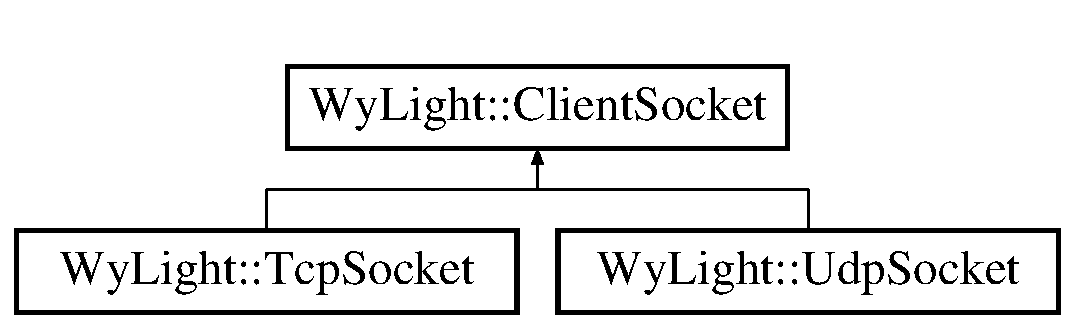
\includegraphics[height=2.000000cm]{class_wy_light_1_1_client_socket}
\end{center}
\end{figure}
\subsection*{Public Member Functions}
\begin{DoxyCompactItemize}
\item 
\hyperlink{class_wy_light_1_1_client_socket_afe4f631abfffc996c24a8a55a9d5cea0}{Client\-Socket} (uint32\-\_\-t addr, uint16\-\_\-t port, int style)  throw (\-Fatal\-Error)
\item 
virtual \hyperlink{class_wy_light_1_1_client_socket_afba3cd05e78cb8f0c46600d3dbba22f4}{$\sim$\-Client\-Socket} ()
\item 
bool \hyperlink{class_wy_light_1_1_client_socket_a8a34f39b3bbd8b4b2901e6c4f6f2d2e9}{Select} (timeval $\ast$timeout) const   throw (\-Fatal\-Error)
\item 
virtual size\-\_\-t \hyperlink{class_wy_light_1_1_client_socket_ab5ea6d042caa7f624015d514263ab6b5}{Send} (const uint8\-\_\-t $\ast$frame, size\-\_\-t length) const =0
\end{DoxyCompactItemize}
\subsection*{Protected Attributes}
\begin{DoxyCompactItemize}
\item 
const int \hyperlink{class_wy_light_1_1_client_socket_a339a7d8dd046156f3d7c148181ac0673}{m\-Sock}
\item 
\hyperlink{struct_wy_light_1_1_ipv4_addr}{Ipv4\-Addr} \hyperlink{class_wy_light_1_1_client_socket_a3849426773c4b3e300edc8cd3b37b16a}{m\-Sock\-Addr}
\end{DoxyCompactItemize}


\subsection{Detailed Description}
Abstract base class controlling the low level socket file descriptor 

\subsection{Constructor \& Destructor Documentation}
\hypertarget{class_wy_light_1_1_client_socket_afe4f631abfffc996c24a8a55a9d5cea0}{\index{Wy\-Light\-::\-Client\-Socket@{Wy\-Light\-::\-Client\-Socket}!Client\-Socket@{Client\-Socket}}
\index{Client\-Socket@{Client\-Socket}!WyLight::ClientSocket@{Wy\-Light\-::\-Client\-Socket}}
\subsubsection[{Client\-Socket}]{\setlength{\rightskip}{0pt plus 5cm}Wy\-Light\-::\-Client\-Socket\-::\-Client\-Socket (
\begin{DoxyParamCaption}
\item[{uint32\-\_\-t}]{addr, }
\item[{uint16\-\_\-t}]{port, }
\item[{int}]{style}
\end{DoxyParamCaption}
)  throw ({\bf Fatal\-Error})}}\label{class_wy_light_1_1_client_socket_afe4f631abfffc996c24a8a55a9d5cea0}
Aquire the low level socket file descriptor 
\begin{DoxyParams}{Parameters}
{\em addr} & I\-Pv4 address in host byte order \\
\hline
{\em port} & I\-Pv4 port number in host byte order \\
\hline
{\em style} & either S\-O\-C\-K\-\_\-\-D\-G\-R\-A\-M (udp) or S\-O\-C\-K\-\_\-\-S\-T\-R\-E\-A\-M for tcp socket \\
\hline
\end{DoxyParams}

\begin{DoxyExceptions}{Exceptions}
{\em \hyperlink{class_wy_light_1_1_fatal_error}{Fatal\-Error}} & if the creation of the bsd sock descriptor fails \\
\hline
\end{DoxyExceptions}
\hypertarget{class_wy_light_1_1_client_socket_afba3cd05e78cb8f0c46600d3dbba22f4}{\index{Wy\-Light\-::\-Client\-Socket@{Wy\-Light\-::\-Client\-Socket}!$\sim$\-Client\-Socket@{$\sim$\-Client\-Socket}}
\index{$\sim$\-Client\-Socket@{$\sim$\-Client\-Socket}!WyLight::ClientSocket@{Wy\-Light\-::\-Client\-Socket}}
\subsubsection[{$\sim$\-Client\-Socket}]{\setlength{\rightskip}{0pt plus 5cm}virtual Wy\-Light\-::\-Client\-Socket\-::$\sim$\-Client\-Socket (
\begin{DoxyParamCaption}
{}
\end{DoxyParamCaption}
)\hspace{0.3cm}{\ttfamily [virtual]}}}\label{class_wy_light_1_1_client_socket_afba3cd05e78cb8f0c46600d3dbba22f4}
Destructor releasing the socket file descriptor 

\subsection{Member Function Documentation}
\hypertarget{class_wy_light_1_1_client_socket_a8a34f39b3bbd8b4b2901e6c4f6f2d2e9}{\index{Wy\-Light\-::\-Client\-Socket@{Wy\-Light\-::\-Client\-Socket}!Select@{Select}}
\index{Select@{Select}!WyLight::ClientSocket@{Wy\-Light\-::\-Client\-Socket}}
\subsubsection[{Select}]{\setlength{\rightskip}{0pt plus 5cm}bool Wy\-Light\-::\-Client\-Socket\-::\-Select (
\begin{DoxyParamCaption}
\item[{timeval $\ast$}]{timeout}
\end{DoxyParamCaption}
) const  throw ({\bf Fatal\-Error})}}\label{class_wy_light_1_1_client_socket_a8a34f39b3bbd8b4b2901e6c4f6f2d2e9}
wait for data on the low level socket 
\begin{DoxyParams}{Parameters}
{\em timeout} & to wait for data, to block indefinitly use N\-U\-L\-L, which is default \\
\hline
\end{DoxyParams}
\begin{DoxyReturn}{Returns}
true if select() timed out, false if data is ready 
\end{DoxyReturn}

\begin{DoxyExceptions}{Exceptions}
{\em \hyperlink{class_wy_light_1_1_fatal_error}{Fatal\-Error}} & if something very unexpected happens \\
\hline
\end{DoxyExceptions}
\hypertarget{class_wy_light_1_1_client_socket_ab5ea6d042caa7f624015d514263ab6b5}{\index{Wy\-Light\-::\-Client\-Socket@{Wy\-Light\-::\-Client\-Socket}!Send@{Send}}
\index{Send@{Send}!WyLight::ClientSocket@{Wy\-Light\-::\-Client\-Socket}}
\subsubsection[{Send}]{\setlength{\rightskip}{0pt plus 5cm}virtual size\-\_\-t Wy\-Light\-::\-Client\-Socket\-::\-Send (
\begin{DoxyParamCaption}
\item[{const uint8\-\_\-t $\ast$}]{frame, }
\item[{size\-\_\-t}]{length}
\end{DoxyParamCaption}
) const\hspace{0.3cm}{\ttfamily [pure virtual]}}}\label{class_wy_light_1_1_client_socket_ab5ea6d042caa7f624015d514263ab6b5}
Interface to send a data frame with a given length, you have to implement this function in child classes 

Implemented in \hyperlink{class_wy_light_1_1_udp_socket_aaba73a044c8aed0ef0c1e44ce46d88ca}{Wy\-Light\-::\-Udp\-Socket}, and \hyperlink{class_wy_light_1_1_tcp_socket_acd2ed7e05e7a8efc55b01e422d957857}{Wy\-Light\-::\-Tcp\-Socket}.



\subsection{Member Data Documentation}
\hypertarget{class_wy_light_1_1_client_socket_a339a7d8dd046156f3d7c148181ac0673}{\index{Wy\-Light\-::\-Client\-Socket@{Wy\-Light\-::\-Client\-Socket}!m\-Sock@{m\-Sock}}
\index{m\-Sock@{m\-Sock}!WyLight::ClientSocket@{Wy\-Light\-::\-Client\-Socket}}
\subsubsection[{m\-Sock}]{\setlength{\rightskip}{0pt plus 5cm}const int Wy\-Light\-::\-Client\-Socket\-::m\-Sock\hspace{0.3cm}{\ttfamily [protected]}}}\label{class_wy_light_1_1_client_socket_a339a7d8dd046156f3d7c148181ac0673}
low level socket file descriptor \hypertarget{class_wy_light_1_1_client_socket_a3849426773c4b3e300edc8cd3b37b16a}{\index{Wy\-Light\-::\-Client\-Socket@{Wy\-Light\-::\-Client\-Socket}!m\-Sock\-Addr@{m\-Sock\-Addr}}
\index{m\-Sock\-Addr@{m\-Sock\-Addr}!WyLight::ClientSocket@{Wy\-Light\-::\-Client\-Socket}}
\subsubsection[{m\-Sock\-Addr}]{\setlength{\rightskip}{0pt plus 5cm}{\bf Ipv4\-Addr} Wy\-Light\-::\-Client\-Socket\-::m\-Sock\-Addr\hspace{0.3cm}{\ttfamily [protected]}}}\label{class_wy_light_1_1_client_socket_a3849426773c4b3e300edc8cd3b37b16a}
I\-Pv4 address of listening or target port 

The documentation for this class was generated from the following file\-:\begin{DoxyCompactItemize}
\item 
library/\hyperlink{_client_socket_8h}{Client\-Socket.\-h}\end{DoxyCompactItemize}

\hypertarget{class_wy_light_1_1_com_proxy}{\section{Wy\-Light\-:\-:Com\-Proxy Class Reference}
\label{class_wy_light_1_1_com_proxy}\index{Wy\-Light\-::\-Com\-Proxy@{Wy\-Light\-::\-Com\-Proxy}}
}


{\ttfamily \#include $<$Com\-Proxy.\-h$>$}

\subsection*{Public Member Functions}
\begin{DoxyCompactItemize}
\item 
\hyperlink{class_wy_light_1_1_com_proxy_a1757ec964a2043668fadb2fb6c7486f7}{Com\-Proxy} (const \hyperlink{class_wy_light_1_1_tcp_socket}{Tcp\-Socket} \&sock)
\item 
size\-\_\-t \hyperlink{class_wy_light_1_1_com_proxy_a56167b55c50edd0a64d5c6826ff9db98}{Send} (const \hyperlink{struct_wy_light_1_1_bl_request}{Bl\-Request} \&req, uint8\-\_\-t $\ast$p\-Response, size\-\_\-t response\-Size, bool do\-Sync=true) const   throw (\-Connection\-Timeout, Fatal\-Error)
\item 
size\-\_\-t \hyperlink{class_wy_light_1_1_com_proxy_aaf78d82cfc84481cd92651299ccb2963}{Send} (const \hyperlink{class_wy_light_1_1_fw_command}{Fw\-Command} \&request, response\-\_\-frame $\ast$p\-Response, size\-\_\-t response\-Size) const   throw (\-Connection\-Timeout, Fatal\-Error)
\end{DoxyCompactItemize}


\subsection{Constructor \& Destructor Documentation}
\hypertarget{class_wy_light_1_1_com_proxy_a1757ec964a2043668fadb2fb6c7486f7}{\index{Wy\-Light\-::\-Com\-Proxy@{Wy\-Light\-::\-Com\-Proxy}!Com\-Proxy@{Com\-Proxy}}
\index{Com\-Proxy@{Com\-Proxy}!WyLight::ComProxy@{Wy\-Light\-::\-Com\-Proxy}}
\subsubsection[{Com\-Proxy}]{\setlength{\rightskip}{0pt plus 5cm}Wy\-Light\-::\-Com\-Proxy\-::\-Com\-Proxy (
\begin{DoxyParamCaption}
\item[{const {\bf Tcp\-Socket} \&}]{sock}
\end{DoxyParamCaption}
)}}\label{class_wy_light_1_1_com_proxy_a1757ec964a2043668fadb2fb6c7486f7}


\subsection{Member Function Documentation}
\hypertarget{class_wy_light_1_1_com_proxy_a56167b55c50edd0a64d5c6826ff9db98}{\index{Wy\-Light\-::\-Com\-Proxy@{Wy\-Light\-::\-Com\-Proxy}!Send@{Send}}
\index{Send@{Send}!WyLight::ComProxy@{Wy\-Light\-::\-Com\-Proxy}}
\subsubsection[{Send}]{\setlength{\rightskip}{0pt plus 5cm}size\-\_\-t Wy\-Light\-::\-Com\-Proxy\-::\-Send (
\begin{DoxyParamCaption}
\item[{const {\bf Bl\-Request} \&}]{req, }
\item[{uint8\-\_\-t $\ast$}]{p\-Response, }
\item[{size\-\_\-t}]{response\-Size, }
\item[{bool}]{do\-Sync = {\ttfamily true}}
\end{DoxyParamCaption}
) const  throw ({\bf Connection\-Timeout}, {\bf Fatal\-Error})}}\label{class_wy_light_1_1_com_proxy_a56167b55c50edd0a64d5c6826ff9db98}
\hypertarget{class_wy_light_1_1_com_proxy_aaf78d82cfc84481cd92651299ccb2963}{\index{Wy\-Light\-::\-Com\-Proxy@{Wy\-Light\-::\-Com\-Proxy}!Send@{Send}}
\index{Send@{Send}!WyLight::ComProxy@{Wy\-Light\-::\-Com\-Proxy}}
\subsubsection[{Send}]{\setlength{\rightskip}{0pt plus 5cm}size\-\_\-t Wy\-Light\-::\-Com\-Proxy\-::\-Send (
\begin{DoxyParamCaption}
\item[{const {\bf Fw\-Command} \&}]{request, }
\item[{response\-\_\-frame $\ast$}]{p\-Response, }
\item[{size\-\_\-t}]{response\-Size}
\end{DoxyParamCaption}
) const  throw ({\bf Connection\-Timeout}, {\bf Fatal\-Error})}}\label{class_wy_light_1_1_com_proxy_aaf78d82cfc84481cd92651299ccb2963}


The documentation for this class was generated from the following file\-:\begin{DoxyCompactItemize}
\item 
library/\hyperlink{_com_proxy_8h}{Com\-Proxy.\-h}\end{DoxyCompactItemize}

\hypertarget{class_wy_light_1_1_connection_lost}{\section{Wy\-Light\-:\-:Connection\-Lost Class Reference}
\label{class_wy_light_1_1_connection_lost}\index{Wy\-Light\-::\-Connection\-Lost@{Wy\-Light\-::\-Connection\-Lost}}
}


{\ttfamily \#include $<$Wifly\-Control\-Exception.\-h$>$}

Inheritance diagram for Wy\-Light\-:\-:Connection\-Lost\-:\begin{figure}[H]
\begin{center}
\leavevmode
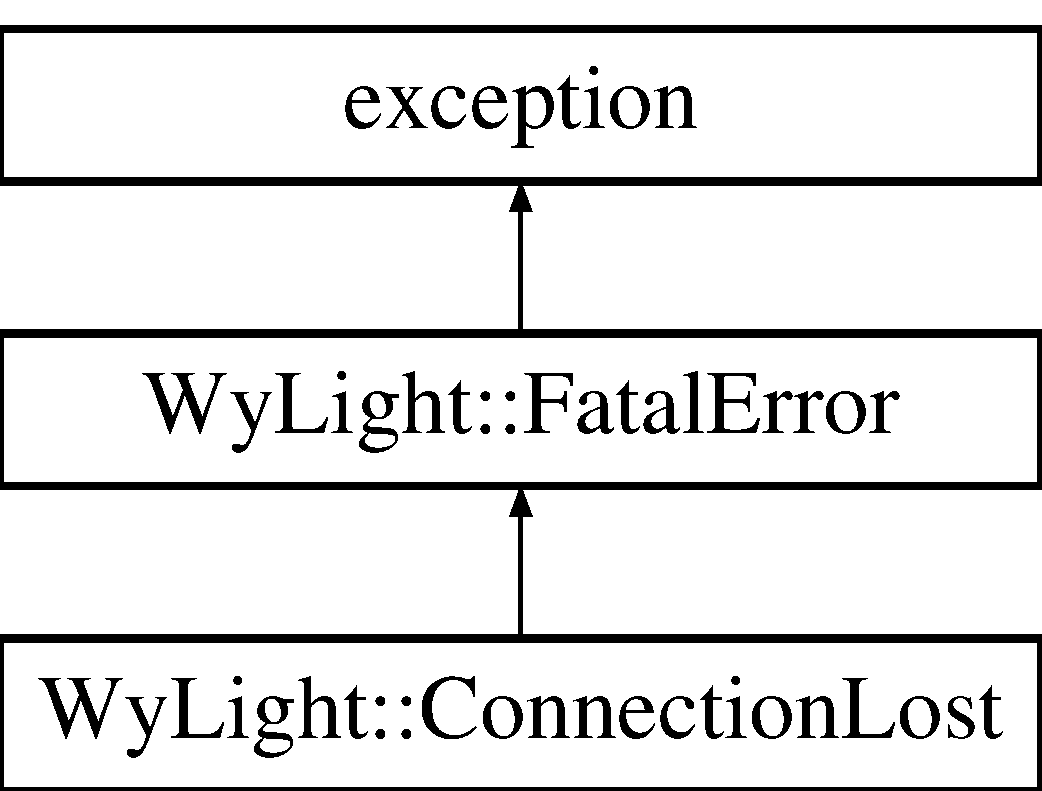
\includegraphics[height=3.000000cm]{class_wy_light_1_1_connection_lost}
\end{center}
\end{figure}
\subsection*{Public Member Functions}
\begin{DoxyCompactItemize}
\item 
\hyperlink{class_wy_light_1_1_connection_lost_a73ee7baed28dc3b7dd34a045a618e259}{Connection\-Lost} (const std\-::string \&description, uint32\-\_\-t addr, uint16\-\_\-t port)
\item 
virtual const char $\ast$ \hyperlink{class_wy_light_1_1_connection_lost_a32dbb008e84c419fdb31b7b4b13b6f7f}{Get\-Java\-Class\-Type} (void) const 
\end{DoxyCompactItemize}
\subsection*{Protected Attributes}
\begin{DoxyCompactItemize}
\item 
uint32\-\_\-t \hyperlink{class_wy_light_1_1_connection_lost_ae4207146ab81928c6ae1a161602a8765}{m\-Address}
\item 
uint16\-\_\-t \hyperlink{class_wy_light_1_1_connection_lost_a54e8b7c58d8f24d8da4fd839aa8e556d}{m\-Port}
\end{DoxyCompactItemize}
\subsection*{Friends}
\begin{DoxyCompactItemize}
\item 
std\-::ostream \& \hyperlink{class_wy_light_1_1_connection_lost_a6a1446a3968cd20190989430f0f441c6}{operator$<$$<$} (std\-::ostream \&out, const \hyperlink{class_wy_light_1_1_connection_lost}{Connection\-Lost} \&ref)
\end{DoxyCompactItemize}


\subsection{Constructor \& Destructor Documentation}
\hypertarget{class_wy_light_1_1_connection_lost_a73ee7baed28dc3b7dd34a045a618e259}{\index{Wy\-Light\-::\-Connection\-Lost@{Wy\-Light\-::\-Connection\-Lost}!Connection\-Lost@{Connection\-Lost}}
\index{Connection\-Lost@{Connection\-Lost}!WyLight::ConnectionLost@{Wy\-Light\-::\-Connection\-Lost}}
\subsubsection[{Connection\-Lost}]{\setlength{\rightskip}{0pt plus 5cm}Wy\-Light\-::\-Connection\-Lost\-::\-Connection\-Lost (
\begin{DoxyParamCaption}
\item[{const std\-::string \&}]{description, }
\item[{uint32\-\_\-t}]{addr, }
\item[{uint16\-\_\-t}]{port}
\end{DoxyParamCaption}
)\hspace{0.3cm}{\ttfamily [inline]}}}\label{class_wy_light_1_1_connection_lost_a73ee7baed28dc3b7dd34a045a618e259}


\subsection{Member Function Documentation}
\hypertarget{class_wy_light_1_1_connection_lost_a32dbb008e84c419fdb31b7b4b13b6f7f}{\index{Wy\-Light\-::\-Connection\-Lost@{Wy\-Light\-::\-Connection\-Lost}!Get\-Java\-Class\-Type@{Get\-Java\-Class\-Type}}
\index{Get\-Java\-Class\-Type@{Get\-Java\-Class\-Type}!WyLight::ConnectionLost@{Wy\-Light\-::\-Connection\-Lost}}
\subsubsection[{Get\-Java\-Class\-Type}]{\setlength{\rightskip}{0pt plus 5cm}virtual const char$\ast$ Wy\-Light\-::\-Connection\-Lost\-::\-Get\-Java\-Class\-Type (
\begin{DoxyParamCaption}
\item[{void}]{}
\end{DoxyParamCaption}
) const\hspace{0.3cm}{\ttfamily [inline]}, {\ttfamily [virtual]}}}\label{class_wy_light_1_1_connection_lost_a32dbb008e84c419fdb31b7b4b13b6f7f}


Reimplemented from \hyperlink{class_wy_light_1_1_fatal_error_aa74decc09fe8aafc15bfbe31f697987a}{Wy\-Light\-::\-Fatal\-Error}.



\subsection{Friends And Related Function Documentation}
\hypertarget{class_wy_light_1_1_connection_lost_a6a1446a3968cd20190989430f0f441c6}{\index{Wy\-Light\-::\-Connection\-Lost@{Wy\-Light\-::\-Connection\-Lost}!operator$<$$<$@{operator$<$$<$}}
\index{operator$<$$<$@{operator$<$$<$}!WyLight::ConnectionLost@{Wy\-Light\-::\-Connection\-Lost}}
\subsubsection[{operator$<$$<$}]{\setlength{\rightskip}{0pt plus 5cm}std\-::ostream\& operator$<$$<$ (
\begin{DoxyParamCaption}
\item[{std\-::ostream \&}]{out, }
\item[{const {\bf Connection\-Lost} \&}]{ref}
\end{DoxyParamCaption}
)\hspace{0.3cm}{\ttfamily [friend]}}}\label{class_wy_light_1_1_connection_lost_a6a1446a3968cd20190989430f0f441c6}


\subsection{Member Data Documentation}
\hypertarget{class_wy_light_1_1_connection_lost_ae4207146ab81928c6ae1a161602a8765}{\index{Wy\-Light\-::\-Connection\-Lost@{Wy\-Light\-::\-Connection\-Lost}!m\-Address@{m\-Address}}
\index{m\-Address@{m\-Address}!WyLight::ConnectionLost@{Wy\-Light\-::\-Connection\-Lost}}
\subsubsection[{m\-Address}]{\setlength{\rightskip}{0pt plus 5cm}uint32\-\_\-t Wy\-Light\-::\-Connection\-Lost\-::m\-Address\hspace{0.3cm}{\ttfamily [protected]}}}\label{class_wy_light_1_1_connection_lost_ae4207146ab81928c6ae1a161602a8765}
\hypertarget{class_wy_light_1_1_connection_lost_a54e8b7c58d8f24d8da4fd839aa8e556d}{\index{Wy\-Light\-::\-Connection\-Lost@{Wy\-Light\-::\-Connection\-Lost}!m\-Port@{m\-Port}}
\index{m\-Port@{m\-Port}!WyLight::ConnectionLost@{Wy\-Light\-::\-Connection\-Lost}}
\subsubsection[{m\-Port}]{\setlength{\rightskip}{0pt plus 5cm}uint16\-\_\-t Wy\-Light\-::\-Connection\-Lost\-::m\-Port\hspace{0.3cm}{\ttfamily [protected]}}}\label{class_wy_light_1_1_connection_lost_a54e8b7c58d8f24d8da4fd839aa8e556d}


The documentation for this class was generated from the following file\-:\begin{DoxyCompactItemize}
\item 
library/\hyperlink{_wifly_control_exception_8h}{Wifly\-Control\-Exception.\-h}\end{DoxyCompactItemize}

\hypertarget{class_wy_light_1_1_connection_timeout}{\section{Wy\-Light\-:\-:Connection\-Timeout Class Reference}
\label{class_wy_light_1_1_connection_timeout}\index{Wy\-Light\-::\-Connection\-Timeout@{Wy\-Light\-::\-Connection\-Timeout}}
}


{\ttfamily \#include $<$Wifly\-Control\-Exception.\-h$>$}

Inheritance diagram for Wy\-Light\-:\-:Connection\-Timeout\-:\begin{figure}[H]
\begin{center}
\leavevmode
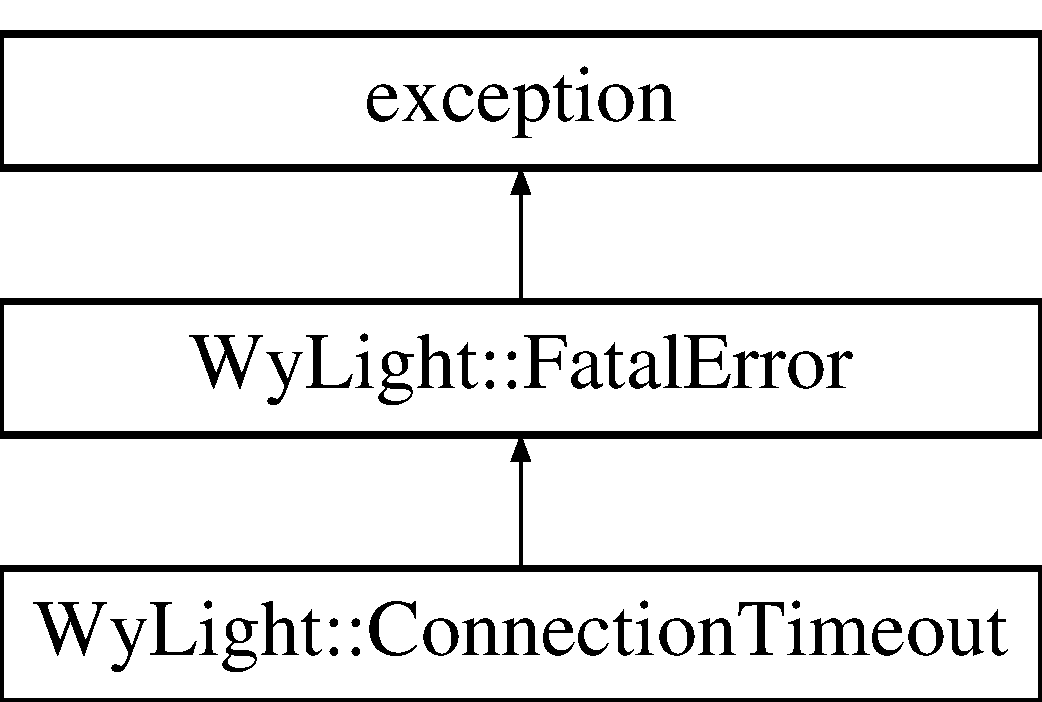
\includegraphics[height=3.000000cm]{class_wy_light_1_1_connection_timeout}
\end{center}
\end{figure}
\subsection*{Public Member Functions}
\begin{DoxyCompactItemize}
\item 
\hyperlink{class_wy_light_1_1_connection_timeout_a462903da2736c79d3015290a8852645c}{Connection\-Timeout} (const std\-::string \&description)
\item 
virtual const char $\ast$ \hyperlink{class_wy_light_1_1_connection_timeout_a2feb264902a3c11a10f4e9eb1ba08bb1}{Get\-Java\-Class\-Type} (void) const 
\end{DoxyCompactItemize}
\subsection*{Additional Inherited Members}


\subsection{Constructor \& Destructor Documentation}
\hypertarget{class_wy_light_1_1_connection_timeout_a462903da2736c79d3015290a8852645c}{\index{Wy\-Light\-::\-Connection\-Timeout@{Wy\-Light\-::\-Connection\-Timeout}!Connection\-Timeout@{Connection\-Timeout}}
\index{Connection\-Timeout@{Connection\-Timeout}!WyLight::ConnectionTimeout@{Wy\-Light\-::\-Connection\-Timeout}}
\subsubsection[{Connection\-Timeout}]{\setlength{\rightskip}{0pt plus 5cm}Wy\-Light\-::\-Connection\-Timeout\-::\-Connection\-Timeout (
\begin{DoxyParamCaption}
\item[{const std\-::string \&}]{description}
\end{DoxyParamCaption}
)\hspace{0.3cm}{\ttfamily [inline]}}}\label{class_wy_light_1_1_connection_timeout_a462903da2736c79d3015290a8852645c}


\subsection{Member Function Documentation}
\hypertarget{class_wy_light_1_1_connection_timeout_a2feb264902a3c11a10f4e9eb1ba08bb1}{\index{Wy\-Light\-::\-Connection\-Timeout@{Wy\-Light\-::\-Connection\-Timeout}!Get\-Java\-Class\-Type@{Get\-Java\-Class\-Type}}
\index{Get\-Java\-Class\-Type@{Get\-Java\-Class\-Type}!WyLight::ConnectionTimeout@{Wy\-Light\-::\-Connection\-Timeout}}
\subsubsection[{Get\-Java\-Class\-Type}]{\setlength{\rightskip}{0pt plus 5cm}virtual const char$\ast$ Wy\-Light\-::\-Connection\-Timeout\-::\-Get\-Java\-Class\-Type (
\begin{DoxyParamCaption}
\item[{void}]{}
\end{DoxyParamCaption}
) const\hspace{0.3cm}{\ttfamily [inline]}, {\ttfamily [virtual]}}}\label{class_wy_light_1_1_connection_timeout_a2feb264902a3c11a10f4e9eb1ba08bb1}


Reimplemented from \hyperlink{class_wy_light_1_1_fatal_error_aa74decc09fe8aafc15bfbe31f697987a}{Wy\-Light\-::\-Fatal\-Error}.



The documentation for this class was generated from the following file\-:\begin{DoxyCompactItemize}
\item 
library/\hyperlink{_wifly_control_exception_8h}{Wifly\-Control\-Exception.\-h}\end{DoxyCompactItemize}

\hypertarget{class_wy_light_1_1_control}{\section{Wy\-Light\-:\-:Control Class Reference}
\label{class_wy_light_1_1_control}\index{Wy\-Light\-::\-Control@{Wy\-Light\-::\-Control}}
}


Class to communicate with a Wifly\-\_\-\-Light Hardware.  




{\ttfamily \#include $<$Wifly\-Control.\-h$>$}

\subsection*{Public Member Functions}
\begin{DoxyCompactItemize}
\item 
\hyperlink{class_wy_light_1_1_control_a2d5efc4402b12961aea578e1aeb91dab}{Control} (uint32\-\_\-t addr, uint16\-\_\-t port)
\item 
void \hyperlink{class_wy_light_1_1_control_a0198560d89e0af7c668ab182d4cd5533}{Bl\-Enable\-Autostart} (void) const   throw (\-Connection\-Timeout, Fatal\-Error)
\item 
void \hyperlink{class_wy_light_1_1_control_a90019ceb9f607dbb3401cfd393a1fe00}{Bl\-Erase\-Eeprom} (void) const   throw (\-Connection\-Timeout, Fatal\-Error)
\item 
void \hyperlink{class_wy_light_1_1_control_ae661b928eb3ddc85614fffb570234bb7}{Bl\-Erase\-Flash} (void) const   throw (\-Connection\-Timeout, Fatal\-Error)
\item 
void \hyperlink{class_wy_light_1_1_control_a8bef060b2d26d436f143784c74750a80}{Bl\-Program\-Flash} (const std\-::string \&filename) const   throw (\-Connection\-Timeout, Fatal\-Error)
\item 
void \hyperlink{class_wy_light_1_1_control_aefe6c849859c10b81620e1251a3acbd0}{Bl\-Read\-Crc\-Flash} (std\-::ostream \&out, uint32\-\_\-t address, size\-\_\-t num\-Bytes) const   throw (\-Connection\-Timeout, Fatal\-Error, Invalid\-Parameter)
\item 
void \hyperlink{class_wy_light_1_1_control_aadac9ad0d311360e2999414cb220c78f}{Bl\-Read\-Eeprom} (std\-::ostream \&out, uint32\-\_\-t address, size\-\_\-t num\-Bytes) const   throw (\-Connection\-Timeout, Fatal\-Error, Invalid\-Parameter)
\item 
void \hyperlink{class_wy_light_1_1_control_ab31a3e0c102ced985377314a3056e588}{Bl\-Read\-Flash} (std\-::ostream \&out, uint32\-\_\-t address, size\-\_\-t num\-Bytes) const   throw (\-Connection\-Timeout, Fatal\-Error, Invalid\-Parameter)
\item 
std\-::string \hyperlink{class_wy_light_1_1_control_ac6329ec0b3f87a0a1538d44fb2e06a4d}{Bl\-Read\-Fw\-Version} (void) const   throw (\-Connection\-Timeout, Fatal\-Error)
\item 
void \hyperlink{class_wy_light_1_1_control_a1d5de392ee1bce3176d0840d855eaa1f}{Bl\-Read\-Info} (\hyperlink{struct_wy_light_1_1_bl_info}{Bl\-Info} \&info) const   throw (\-Connection\-Timeout, Fatal\-Error)
\item 
void \hyperlink{class_wy_light_1_1_control_a6a515497781d7ab7ad5fde04b5466c63}{Bl\-Run\-App} (void) const   throw (\-Connection\-Timeout, Fatal\-Error)
\item 
std\-::string \hyperlink{class_wy_light_1_1_control_a32fce52c7c113c90654e6835c0274f73}{Conf\-Get\-Device\-Id} (void) const 
\item 
std\-::string \hyperlink{class_wy_light_1_1_control_adc559100e686136cff2c3bfea53f55a3}{Conf\-Get\-Passphrase} (void) const 
\item 
bool \hyperlink{class_wy_light_1_1_control_a08764c74e17d008cf9e03ae6c9a145e0}{Conf\-Get\-Soft\-Ap} (void) const 
\item 
std\-::string \hyperlink{class_wy_light_1_1_control_a9128e80172dcb8586c9821dc7587f122}{Conf\-Get\-Ssid} (void) const 
\item 
bool \hyperlink{class_wy_light_1_1_control_a16a660f58bf48a006e1709a28ebc2ae8}{Conf\-Module\-As\-Soft\-A\-P} (const std\-::string \&accesspoint\-Name=\char`\"{}Wifly\-\_\-\-Light\char`\"{}) const 
\item 
bool \hyperlink{class_wy_light_1_1_control_a801a17d49dc76e80a2a8ea8709e4d6f5}{Conf\-Module\-For\-Wlan} (const std\-::string \&phrase, const std\-::string \&ssid, const std\-::string \&device\-Id=\char`\"{}Wifly\-\_\-\-Light\char`\"{}) const 
\item 
bool \hyperlink{class_wy_light_1_1_control_aa9ac31328f888ff1d90cefe04f7353e6}{Conf\-Reboot\-Wlan\-Module} (void) const 
\item 
bool \hyperlink{class_wy_light_1_1_control_aa829e0a757758eb960da902803b138d8}{Conf\-Set\-Device\-Id} (const std\-::string \&name) const 
\item 
bool \hyperlink{class_wy_light_1_1_control_a9079d8f3560a5c811bf97b138ad12155}{Conf\-Change\-Wlan\-Channel} (void) const 
\item 
std\-::string \hyperlink{class_wy_light_1_1_control_aedce9e77a3358f551cc66c4a8a492260}{Fw\-Get\-Cycletime} (void)  throw (\-Connection\-Timeout, Fatal\-Error, Script\-Buffer\-Full)
\item 
void \hyperlink{class_wy_light_1_1_control_a9a082452281e1de4160b1fa9f1275a91}{Fw\-Get\-Rtc} (tm \&time\-Value)  throw (\-Connection\-Timeout, Fatal\-Error, Script\-Buffer\-Full)
\item 
std\-::string \hyperlink{class_wy_light_1_1_control_af2035569a368fbcafa758ec649914f66}{Fw\-Get\-Tracebuffer} (void)  throw (\-Connection\-Timeout, Fatal\-Error, Script\-Buffer\-Full)
\item 
std\-::string \hyperlink{class_wy_light_1_1_control_adb78c0d47ab18019b4e5758df6796062}{Fw\-Get\-Version} (void)  throw (\-Connection\-Timeout, Fatal\-Error, Script\-Buffer\-Full)
\item 
void \hyperlink{class_wy_light_1_1_control_a4a4621f063e3d539f06d4e1141229e44}{Fw\-Test} (void)
\item 
void \hyperlink{class_wy_light_1_1_control_af2f20a5d9d87b9b1c8a2e481e71602a8}{Fw\-Stress\-Test} (void)
\item 
\hyperlink{class_wy_light_1_1_control}{Control} \& \hyperlink{class_wy_light_1_1_control_a3679510a5c28c97ef9cbbbbc2ffee9e8}{operator$<$$<$} (\hyperlink{class_wy_light_1_1_fw_command}{Fw\-Command} \&\&cmd)  throw (\-Connection\-Timeout, Fatal\-Error, Script\-Buffer\-Full)
\item 
\hyperlink{class_wy_light_1_1_control}{Control} \& \hyperlink{class_wy_light_1_1_control_ab0948069a02431beb689055b56afc759}{operator$<$$<$} (\hyperlink{class_wy_light_1_1_fw_command}{Fw\-Command} \&cmd)  throw (\-Connection\-Timeout, Fatal\-Error, Script\-Buffer\-Full)
\item 
\hyperlink{class_wy_light_1_1_control}{Control} \& \hyperlink{class_wy_light_1_1_control_add8b6887c1fb93571af763d436193f7e}{operator$<$$<$} (\hyperlink{class_wy_light_1_1_script}{Script} \&\&script)  throw (\-Connection\-Timeout, Fatal\-Error, Script\-Buffer\-Full)
\item 
\hyperlink{class_wy_light_1_1_control}{Control} \& \hyperlink{class_wy_light_1_1_control_abd06c7b743976e2c0f345e22fd2f5a2a}{operator$<$$<$} (\hyperlink{class_wy_light_1_1_script}{Script} \&script)  throw (\-Connection\-Timeout, Fatal\-Error, Script\-Buffer\-Full)
\item 
std\-::string \hyperlink{class_wy_light_1_1_control_a09d8a865f5557d584032cf088e32ade0}{Extract\-Fw\-Version} (const std\-::string \&p\-Filename) const 
\end{DoxyCompactItemize}
\subsection*{Static Public Attributes}
\begin{DoxyCompactItemize}
\item 
static const std\-::string \hyperlink{class_wy_light_1_1_control_a6d407aadfe5921e4af9bf756cc9d8a28}{L\-E\-D\-S\-\_\-\-A\-L\-L}
\end{DoxyCompactItemize}
\subsection*{Friends}
\begin{DoxyCompactItemize}
\item 
size\-\_\-t \hyperlink{class_wy_light_1_1_control_a327c95f9335fa4b257b064ef2e917a80}{ut\-\_\-\-Wifly\-Control\-\_\-\-Bl\-Eeprom\-Write} (void)
\item 
size\-\_\-t \hyperlink{class_wy_light_1_1_control_a661b9ec8a685bc800221f2fd5d031a20}{ut\-\_\-\-Wifly\-Control\-\_\-\-Bl\-Flash\-Write} (void)
\item 
size\-\_\-t \hyperlink{class_wy_light_1_1_control_aeefa8ad693af2b134456faaf1586a2f7}{ut\-\_\-\-Wifly\-Control\-\_\-\-Conf\-Set\-Defaults} (void)
\item 
size\-\_\-t \hyperlink{class_wy_light_1_1_control_a04989feb17717c76d1dd95666aec3c93}{ut\-\_\-\-Wifly\-Control\-\_\-\-Conf\-Set\-Wlan} (void)
\end{DoxyCompactItemize}


\subsection{Detailed Description}
Class to communicate with a Wifly\-\_\-\-Light Hardware. 

The \hyperlink{class_wy_light_1_1_control}{Control} class allows the user to control the Wifly\-\_\-\-Light Hardware. There are three target's at the Wifly\-\_\-\-Light Hardware.
\begin{DoxyItemize}
\item Bootloader\par
 All methodes with Bl$\ast$ relate to the bootloader part.
\item Firmware\par
 All methodes with Fw$\ast$ relate to the firmware part.
\item R\-N-\/171 Wifi Interface\par
 All methodes witch Conf$\ast$ relate to the communication module. 
\end{DoxyItemize}

\subsection{Constructor \& Destructor Documentation}
\hypertarget{class_wy_light_1_1_control_a2d5efc4402b12961aea578e1aeb91dab}{\index{Wy\-Light\-::\-Control@{Wy\-Light\-::\-Control}!Control@{Control}}
\index{Control@{Control}!WyLight::Control@{Wy\-Light\-::\-Control}}
\subsubsection[{Control}]{\setlength{\rightskip}{0pt plus 5cm}Wy\-Light\-::\-Control\-::\-Control (
\begin{DoxyParamCaption}
\item[{uint32\-\_\-t}]{addr, }
\item[{uint16\-\_\-t}]{port}
\end{DoxyParamCaption}
)}}\label{class_wy_light_1_1_control_a2d5efc4402b12961aea578e1aeb91dab}
Connect to a wifly device 
\begin{DoxyParams}{Parameters}
{\em addr} & ipv4 address as 32 bit value in host byte order \\
\hline
{\em port} & number of the wifly device server in host byte order \\
\hline
\end{DoxyParams}


\subsection{Member Function Documentation}
\hypertarget{class_wy_light_1_1_control_a0198560d89e0af7c668ab182d4cd5533}{\index{Wy\-Light\-::\-Control@{Wy\-Light\-::\-Control}!Bl\-Enable\-Autostart@{Bl\-Enable\-Autostart}}
\index{Bl\-Enable\-Autostart@{Bl\-Enable\-Autostart}!WyLight::Control@{Wy\-Light\-::\-Control}}
\subsubsection[{Bl\-Enable\-Autostart}]{\setlength{\rightskip}{0pt plus 5cm}void Wy\-Light\-::\-Control\-::\-Bl\-Enable\-Autostart (
\begin{DoxyParamCaption}
\item[{void}]{}
\end{DoxyParamCaption}
) const  throw ({\bf Connection\-Timeout}, {\bf Fatal\-Error})}}\label{class_wy_light_1_1_control_a0198560d89e0af7c668ab182d4cd5533}
Instructs the bootloader to set the autostart flag to true. This ensures the bootloader will be started on the next reboot automatically. 
\begin{DoxyExceptions}{Exceptions}
{\em \hyperlink{class_wy_light_1_1_connection_timeout}{Connection\-Timeout}} & if response timed out \\
\hline
{\em \hyperlink{class_wy_light_1_1_fatal_error}{Fatal\-Error}} & if command code of the response doesn't match the code of the request, or too many retries failed \\
\hline
{\em \hyperlink{class_wy_light_1_1_invalid_parameter}{Invalid\-Parameter}} & a parameter is out of bound \\
\hline
\end{DoxyExceptions}
\hypertarget{class_wy_light_1_1_control_a90019ceb9f607dbb3401cfd393a1fe00}{\index{Wy\-Light\-::\-Control@{Wy\-Light\-::\-Control}!Bl\-Erase\-Eeprom@{Bl\-Erase\-Eeprom}}
\index{Bl\-Erase\-Eeprom@{Bl\-Erase\-Eeprom}!WyLight::Control@{Wy\-Light\-::\-Control}}
\subsubsection[{Bl\-Erase\-Eeprom}]{\setlength{\rightskip}{0pt plus 5cm}void Wy\-Light\-::\-Control\-::\-Bl\-Erase\-Eeprom (
\begin{DoxyParamCaption}
\item[{void}]{}
\end{DoxyParamCaption}
) const  throw ({\bf Connection\-Timeout}, {\bf Fatal\-Error})}}\label{class_wy_light_1_1_control_a90019ceb9f607dbb3401cfd393a1fe00}
Instructs the bootloader to erase the whole eeprom. The wifly device has to be in bootloader mode for this command. 
\begin{DoxyExceptions}{Exceptions}
{\em \hyperlink{class_wy_light_1_1_connection_timeout}{Connection\-Timeout}} & if response timed out \\
\hline
{\em \hyperlink{class_wy_light_1_1_fatal_error}{Fatal\-Error}} & if command code of the response doesn't match the code of the request, or too many retries failed \\
\hline
{\em \hyperlink{class_wy_light_1_1_invalid_parameter}{Invalid\-Parameter}} & a parameter is out of bound \\
\hline
\end{DoxyExceptions}
\hypertarget{class_wy_light_1_1_control_ae661b928eb3ddc85614fffb570234bb7}{\index{Wy\-Light\-::\-Control@{Wy\-Light\-::\-Control}!Bl\-Erase\-Flash@{Bl\-Erase\-Flash}}
\index{Bl\-Erase\-Flash@{Bl\-Erase\-Flash}!WyLight::Control@{Wy\-Light\-::\-Control}}
\subsubsection[{Bl\-Erase\-Flash}]{\setlength{\rightskip}{0pt plus 5cm}void Wy\-Light\-::\-Control\-::\-Bl\-Erase\-Flash (
\begin{DoxyParamCaption}
\item[{void}]{}
\end{DoxyParamCaption}
) const  throw ({\bf Connection\-Timeout}, {\bf Fatal\-Error})}}\label{class_wy_light_1_1_control_ae661b928eb3ddc85614fffb570234bb7}
Instructs the bootloader to erase the whole flash which is not occupied by the bootloader itself. The wifly device has to be in bootloader mode for this command. 
\begin{DoxyExceptions}{Exceptions}
{\em \hyperlink{class_wy_light_1_1_connection_timeout}{Connection\-Timeout}} & if response timed out \\
\hline
{\em \hyperlink{class_wy_light_1_1_fatal_error}{Fatal\-Error}} & if command code of the response doesn't match the code of the request, or too many retries failed \\
\hline
\end{DoxyExceptions}
\hypertarget{class_wy_light_1_1_control_a8bef060b2d26d436f143784c74750a80}{\index{Wy\-Light\-::\-Control@{Wy\-Light\-::\-Control}!Bl\-Program\-Flash@{Bl\-Program\-Flash}}
\index{Bl\-Program\-Flash@{Bl\-Program\-Flash}!WyLight::Control@{Wy\-Light\-::\-Control}}
\subsubsection[{Bl\-Program\-Flash}]{\setlength{\rightskip}{0pt plus 5cm}void Wy\-Light\-::\-Control\-::\-Bl\-Program\-Flash (
\begin{DoxyParamCaption}
\item[{const std\-::string \&}]{filename}
\end{DoxyParamCaption}
) const  throw ({\bf Connection\-Timeout}, {\bf Fatal\-Error})}}\label{class_wy_light_1_1_control_a8bef060b2d26d436f143784c74750a80}
Instructs the bootloader to update the wifly device with new firmware. The wifly device has to be in bootloader mode for this command. 
\begin{DoxyParams}{Parameters}
{\em filename} & path to the $\ast$.hex file containing the new firmware \\
\hline
\end{DoxyParams}

\begin{DoxyExceptions}{Exceptions}
{\em \hyperlink{class_wy_light_1_1_connection_timeout}{Connection\-Timeout}} & if response timed out \\
\hline
{\em \hyperlink{class_wy_light_1_1_fatal_error}{Fatal\-Error}} & if command code of the response doesn't match the code of the request, or too many retries failed \\
\hline
\end{DoxyExceptions}
\hypertarget{class_wy_light_1_1_control_aefe6c849859c10b81620e1251a3acbd0}{\index{Wy\-Light\-::\-Control@{Wy\-Light\-::\-Control}!Bl\-Read\-Crc\-Flash@{Bl\-Read\-Crc\-Flash}}
\index{Bl\-Read\-Crc\-Flash@{Bl\-Read\-Crc\-Flash}!WyLight::Control@{Wy\-Light\-::\-Control}}
\subsubsection[{Bl\-Read\-Crc\-Flash}]{\setlength{\rightskip}{0pt plus 5cm}void Wy\-Light\-::\-Control\-::\-Bl\-Read\-Crc\-Flash (
\begin{DoxyParamCaption}
\item[{std\-::ostream \&}]{out, }
\item[{uint32\-\_\-t}]{address, }
\item[{size\-\_\-t}]{num\-Bytes}
\end{DoxyParamCaption}
) const  throw ({\bf Connection\-Timeout}, {\bf Fatal\-Error}, {\bf Invalid\-Parameter})}}\label{class_wy_light_1_1_control_aefe6c849859c10b81620e1251a3acbd0}
Instructs the bootloader to create crc-\/16 checksums for the content of the specified flash area. T\-O\-D\-O crc values are in little endian byte order The wifly device has to be in bootloader mode for this command. 
\begin{DoxyParams}{Parameters}
{\em out} & ostream for the resulting 16bit crc values \\
\hline
{\em address} & crc generation starts from this flash address \\
\hline
{\em num\-Bytes} & size of the flash area for which the crc are calculated \\
\hline
\end{DoxyParams}

\begin{DoxyExceptions}{Exceptions}
{\em \hyperlink{class_wy_light_1_1_connection_timeout}{Connection\-Timeout}} & if response timed out \\
\hline
{\em \hyperlink{class_wy_light_1_1_fatal_error}{Fatal\-Error}} & if command code of the response doesn't match the code of the request, or too many retries failed \\
\hline
{\em \hyperlink{class_wy_light_1_1_invalid_parameter}{Invalid\-Parameter}} & a parameter is out of bound \\
\hline
\end{DoxyExceptions}
\hypertarget{class_wy_light_1_1_control_aadac9ad0d311360e2999414cb220c78f}{\index{Wy\-Light\-::\-Control@{Wy\-Light\-::\-Control}!Bl\-Read\-Eeprom@{Bl\-Read\-Eeprom}}
\index{Bl\-Read\-Eeprom@{Bl\-Read\-Eeprom}!WyLight::Control@{Wy\-Light\-::\-Control}}
\subsubsection[{Bl\-Read\-Eeprom}]{\setlength{\rightskip}{0pt plus 5cm}void Wy\-Light\-::\-Control\-::\-Bl\-Read\-Eeprom (
\begin{DoxyParamCaption}
\item[{std\-::ostream \&}]{out, }
\item[{uint32\-\_\-t}]{address, }
\item[{size\-\_\-t}]{num\-Bytes}
\end{DoxyParamCaption}
) const  throw ({\bf Connection\-Timeout}, {\bf Fatal\-Error}, {\bf Invalid\-Parameter})}}\label{class_wy_light_1_1_control_aadac9ad0d311360e2999414cb220c78f}
Instructs the bootloader to read the specified memory area of the eeprom. The wifly device has to be in bootloader mode for this command. 
\begin{DoxyParams}{Parameters}
{\em out} & ostream where the eeprom content is written \\
\hline
{\em address} & start of the eeprom region to read \\
\hline
{\em num\-Bytes} & size of the eeprom region to read \\
\hline
\end{DoxyParams}

\begin{DoxyExceptions}{Exceptions}
{\em \hyperlink{class_wy_light_1_1_connection_timeout}{Connection\-Timeout}} & if response timed out \\
\hline
{\em \hyperlink{class_wy_light_1_1_fatal_error}{Fatal\-Error}} & if command code of the response doesn't match the code of the request, or too many retries failed \\
\hline
{\em \hyperlink{class_wy_light_1_1_invalid_parameter}{Invalid\-Parameter}} & a parameter is out of bound \\
\hline
\end{DoxyExceptions}
\hypertarget{class_wy_light_1_1_control_ab31a3e0c102ced985377314a3056e588}{\index{Wy\-Light\-::\-Control@{Wy\-Light\-::\-Control}!Bl\-Read\-Flash@{Bl\-Read\-Flash}}
\index{Bl\-Read\-Flash@{Bl\-Read\-Flash}!WyLight::Control@{Wy\-Light\-::\-Control}}
\subsubsection[{Bl\-Read\-Flash}]{\setlength{\rightskip}{0pt plus 5cm}void Wy\-Light\-::\-Control\-::\-Bl\-Read\-Flash (
\begin{DoxyParamCaption}
\item[{std\-::ostream \&}]{out, }
\item[{uint32\-\_\-t}]{address, }
\item[{size\-\_\-t}]{num\-Bytes}
\end{DoxyParamCaption}
) const  throw ({\bf Connection\-Timeout}, {\bf Fatal\-Error}, {\bf Invalid\-Parameter})}}\label{class_wy_light_1_1_control_ab31a3e0c102ced985377314a3056e588}
Instructs the bootloader to read the specified memory area of the flash. The wifly device has to be in bootloader mode for this command. 
\begin{DoxyParams}{Parameters}
{\em out} & ostream where the flash content is written \\
\hline
{\em address} & start of the flash region to read \\
\hline
{\em num\-Bytes} & size of the flash region to read \\
\hline
\end{DoxyParams}

\begin{DoxyExceptions}{Exceptions}
{\em \hyperlink{class_wy_light_1_1_connection_timeout}{Connection\-Timeout}} & if response timed out \\
\hline
{\em \hyperlink{class_wy_light_1_1_fatal_error}{Fatal\-Error}} & if command code of the response doesn't match the code of the request, or too many retries failed \\
\hline
{\em \hyperlink{class_wy_light_1_1_invalid_parameter}{Invalid\-Parameter}} & a parameter is out of bound \\
\hline
\end{DoxyExceptions}
\hypertarget{class_wy_light_1_1_control_ac6329ec0b3f87a0a1538d44fb2e06a4d}{\index{Wy\-Light\-::\-Control@{Wy\-Light\-::\-Control}!Bl\-Read\-Fw\-Version@{Bl\-Read\-Fw\-Version}}
\index{Bl\-Read\-Fw\-Version@{Bl\-Read\-Fw\-Version}!WyLight::Control@{Wy\-Light\-::\-Control}}
\subsubsection[{Bl\-Read\-Fw\-Version}]{\setlength{\rightskip}{0pt plus 5cm}std\-::string Wy\-Light\-::\-Control\-::\-Bl\-Read\-Fw\-Version (
\begin{DoxyParamCaption}
\item[{void}]{}
\end{DoxyParamCaption}
) const  throw ({\bf Connection\-Timeout}, {\bf Fatal\-Error})}}\label{class_wy_light_1_1_control_ac6329ec0b3f87a0a1538d44fb2e06a4d}
Instructs the bootloader to read the version string from the firmware memory. The wifly device has to be in bootloader mode for this command. \begin{DoxyReturn}{Returns}
the version string from pic flash memory 
\end{DoxyReturn}

\begin{DoxyExceptions}{Exceptions}
{\em \hyperlink{class_wy_light_1_1_connection_timeout}{Connection\-Timeout}} & if response timed out \\
\hline
{\em \hyperlink{class_wy_light_1_1_fatal_error}{Fatal\-Error}} & if command code of the response doesn't match the code of the request, or too many retries failed \\
\hline
\end{DoxyExceptions}
\hypertarget{class_wy_light_1_1_control_a1d5de392ee1bce3176d0840d855eaa1f}{\index{Wy\-Light\-::\-Control@{Wy\-Light\-::\-Control}!Bl\-Read\-Info@{Bl\-Read\-Info}}
\index{Bl\-Read\-Info@{Bl\-Read\-Info}!WyLight::Control@{Wy\-Light\-::\-Control}}
\subsubsection[{Bl\-Read\-Info}]{\setlength{\rightskip}{0pt plus 5cm}void Wy\-Light\-::\-Control\-::\-Bl\-Read\-Info (
\begin{DoxyParamCaption}
\item[{{\bf Bl\-Info} \&}]{info}
\end{DoxyParamCaption}
) const  throw ({\bf Connection\-Timeout}, {\bf Fatal\-Error})}}\label{class_wy_light_1_1_control_a1d5de392ee1bce3176d0840d855eaa1f}
Instructs the bootloader to return a struct of bootloader informations like bootloader version, flash and eeprom size. see $<$\hyperlink{struct_wy_light_1_1_bl_info}{Bl\-Info}$>$ for details. The wifly device has to be in bootloader mode for this command. 
\begin{DoxyExceptions}{Exceptions}
{\em \hyperlink{class_wy_light_1_1_connection_timeout}{Connection\-Timeout}} & if response timed out \\
\hline
{\em \hyperlink{class_wy_light_1_1_fatal_error}{Fatal\-Error}} & if command code of the response doesn't match the code of the request, or too many retries failed \\
\hline
\end{DoxyExceptions}
\hypertarget{class_wy_light_1_1_control_a6a515497781d7ab7ad5fde04b5466c63}{\index{Wy\-Light\-::\-Control@{Wy\-Light\-::\-Control}!Bl\-Run\-App@{Bl\-Run\-App}}
\index{Bl\-Run\-App@{Bl\-Run\-App}!WyLight::Control@{Wy\-Light\-::\-Control}}
\subsubsection[{Bl\-Run\-App}]{\setlength{\rightskip}{0pt plus 5cm}void Wy\-Light\-::\-Control\-::\-Bl\-Run\-App (
\begin{DoxyParamCaption}
\item[{void}]{}
\end{DoxyParamCaption}
) const  throw ({\bf Connection\-Timeout}, {\bf Fatal\-Error})}}\label{class_wy_light_1_1_control_a6a515497781d7ab7ad5fde04b5466c63}
Instructs the bootloader to start the wifly device firmware. The wifly device has to be in bootloader mode for this command. 
\begin{DoxyExceptions}{Exceptions}
{\em \hyperlink{class_wy_light_1_1_connection_timeout}{Connection\-Timeout}} & if response timed out \\
\hline
{\em \hyperlink{class_wy_light_1_1_fatal_error}{Fatal\-Error}} & if command code of the response doesn't match the code of the request, or too many retries failed \\
\hline
\end{DoxyExceptions}
\hypertarget{class_wy_light_1_1_control_a9079d8f3560a5c811bf97b138ad12155}{\index{Wy\-Light\-::\-Control@{Wy\-Light\-::\-Control}!Conf\-Change\-Wlan\-Channel@{Conf\-Change\-Wlan\-Channel}}
\index{Conf\-Change\-Wlan\-Channel@{Conf\-Change\-Wlan\-Channel}!WyLight::Control@{Wy\-Light\-::\-Control}}
\subsubsection[{Conf\-Change\-Wlan\-Channel}]{\setlength{\rightskip}{0pt plus 5cm}bool Wy\-Light\-::\-Control\-::\-Conf\-Change\-Wlan\-Channel (
\begin{DoxyParamCaption}
\item[{void}]{}
\end{DoxyParamCaption}
) const}}\label{class_wy_light_1_1_control_a9079d8f3560a5c811bf97b138ad12155}
Wlan module performs a wifi scan and changes to the next free channel. This function can take some time. \begin{DoxyReturn}{Returns}
false, in case of an error 
\end{DoxyReturn}
\hypertarget{class_wy_light_1_1_control_a32fce52c7c113c90654e6835c0274f73}{\index{Wy\-Light\-::\-Control@{Wy\-Light\-::\-Control}!Conf\-Get\-Device\-Id@{Conf\-Get\-Device\-Id}}
\index{Conf\-Get\-Device\-Id@{Conf\-Get\-Device\-Id}!WyLight::Control@{Wy\-Light\-::\-Control}}
\subsubsection[{Conf\-Get\-Device\-Id}]{\setlength{\rightskip}{0pt plus 5cm}std\-::string Wy\-Light\-::\-Control\-::\-Conf\-Get\-Device\-Id (
\begin{DoxyParamCaption}
\item[{void}]{}
\end{DoxyParamCaption}
) const}}\label{class_wy_light_1_1_control_a32fce52c7c113c90654e6835c0274f73}
Read the device id from \hyperlink{namespace_wy_light}{Wy\-Light} module \begin{DoxyReturn}{Returns}
an empty string or the device id 
\end{DoxyReturn}
\hypertarget{class_wy_light_1_1_control_adc559100e686136cff2c3bfea53f55a3}{\index{Wy\-Light\-::\-Control@{Wy\-Light\-::\-Control}!Conf\-Get\-Passphrase@{Conf\-Get\-Passphrase}}
\index{Conf\-Get\-Passphrase@{Conf\-Get\-Passphrase}!WyLight::Control@{Wy\-Light\-::\-Control}}
\subsubsection[{Conf\-Get\-Passphrase}]{\setlength{\rightskip}{0pt plus 5cm}std\-::string Wy\-Light\-::\-Control\-::\-Conf\-Get\-Passphrase (
\begin{DoxyParamCaption}
\item[{void}]{}
\end{DoxyParamCaption}
) const}}\label{class_wy_light_1_1_control_adc559100e686136cff2c3bfea53f55a3}
Read the currently configured wlan passphrase from \hyperlink{namespace_wy_light}{Wy\-Light} module \begin{DoxyReturn}{Returns}
an empty string or the wlan passphrase 
\end{DoxyReturn}
\hypertarget{class_wy_light_1_1_control_a08764c74e17d008cf9e03ae6c9a145e0}{\index{Wy\-Light\-::\-Control@{Wy\-Light\-::\-Control}!Conf\-Get\-Soft\-Ap@{Conf\-Get\-Soft\-Ap}}
\index{Conf\-Get\-Soft\-Ap@{Conf\-Get\-Soft\-Ap}!WyLight::Control@{Wy\-Light\-::\-Control}}
\subsubsection[{Conf\-Get\-Soft\-Ap}]{\setlength{\rightskip}{0pt plus 5cm}bool Wy\-Light\-::\-Control\-::\-Conf\-Get\-Soft\-Ap (
\begin{DoxyParamCaption}
\item[{void}]{}
\end{DoxyParamCaption}
) const}}\label{class_wy_light_1_1_control_a08764c74e17d008cf9e03ae6c9a145e0}
Read the currently configured mode(client/\-Soft\-A\-P) from \hyperlink{namespace_wy_light}{Wy\-Light} module \begin{DoxyReturn}{Returns}
true if \hyperlink{namespace_wy_light}{Wy\-Light} module is configured for Soft\-A\-P mode 
\end{DoxyReturn}
\hypertarget{class_wy_light_1_1_control_a9128e80172dcb8586c9821dc7587f122}{\index{Wy\-Light\-::\-Control@{Wy\-Light\-::\-Control}!Conf\-Get\-Ssid@{Conf\-Get\-Ssid}}
\index{Conf\-Get\-Ssid@{Conf\-Get\-Ssid}!WyLight::Control@{Wy\-Light\-::\-Control}}
\subsubsection[{Conf\-Get\-Ssid}]{\setlength{\rightskip}{0pt plus 5cm}std\-::string Wy\-Light\-::\-Control\-::\-Conf\-Get\-Ssid (
\begin{DoxyParamCaption}
\item[{void}]{}
\end{DoxyParamCaption}
) const}}\label{class_wy_light_1_1_control_a9128e80172dcb8586c9821dc7587f122}
Read the currently configured ssid from \hyperlink{namespace_wy_light}{Wy\-Light} module \begin{DoxyReturn}{Returns}
an empty string or the ssid 
\end{DoxyReturn}
\hypertarget{class_wy_light_1_1_control_a16a660f58bf48a006e1709a28ebc2ae8}{\index{Wy\-Light\-::\-Control@{Wy\-Light\-::\-Control}!Conf\-Module\-As\-Soft\-A\-P@{Conf\-Module\-As\-Soft\-A\-P}}
\index{Conf\-Module\-As\-Soft\-A\-P@{Conf\-Module\-As\-Soft\-A\-P}!WyLight::Control@{Wy\-Light\-::\-Control}}
\subsubsection[{Conf\-Module\-As\-Soft\-A\-P}]{\setlength{\rightskip}{0pt plus 5cm}bool Wy\-Light\-::\-Control\-::\-Conf\-Module\-As\-Soft\-A\-P (
\begin{DoxyParamCaption}
\item[{const std\-::string \&}]{accesspoint\-Name = {\ttfamily \char`\"{}Wifly\-\_\-Light\char`\"{}}}
\end{DoxyParamCaption}
) const}}\label{class_wy_light_1_1_control_a16a660f58bf48a006e1709a28ebc2ae8}
Configurates the \hyperlink{namespace_wy_light}{Wy\-Light} module as stand alone accesspoint. With accesspoint name you can change the ssid for this accesspoint. 
\begin{DoxyParams}{Parameters}
{\em accesspoint\-Name} & 1 -\/ 32 characters \\
\hline
\end{DoxyParams}
\begin{DoxyReturn}{Returns}
false, in case of an error 
\end{DoxyReturn}
\hypertarget{class_wy_light_1_1_control_a801a17d49dc76e80a2a8ea8709e4d6f5}{\index{Wy\-Light\-::\-Control@{Wy\-Light\-::\-Control}!Conf\-Module\-For\-Wlan@{Conf\-Module\-For\-Wlan}}
\index{Conf\-Module\-For\-Wlan@{Conf\-Module\-For\-Wlan}!WyLight::Control@{Wy\-Light\-::\-Control}}
\subsubsection[{Conf\-Module\-For\-Wlan}]{\setlength{\rightskip}{0pt plus 5cm}bool Wy\-Light\-::\-Control\-::\-Conf\-Module\-For\-Wlan (
\begin{DoxyParamCaption}
\item[{const std\-::string \&}]{phrase, }
\item[{const std\-::string \&}]{ssid, }
\item[{const std\-::string \&}]{device\-Id = {\ttfamily \char`\"{}Wifly\-\_\-Light\char`\"{}}}
\end{DoxyParamCaption}
) const}}\label{class_wy_light_1_1_control_a801a17d49dc76e80a2a8ea8709e4d6f5}
Configurates the \hyperlink{namespace_wy_light}{Wy\-Light} module as client for an existing wlan network with W\-P\-A2 protection 
\begin{DoxyParams}{Parameters}
{\em phrase} & W\-P\-A2 passphrase 1 -\/ 63 characters \\
\hline
{\em ssid} & 1 -\/ 32 characters \\
\hline
{\em device\-Id} & 1 -\/ 32 characters, unique name which apperas in the broadcast message \\
\hline
\end{DoxyParams}
\begin{DoxyReturn}{Returns}
false, in case of an error 
\end{DoxyReturn}
\hypertarget{class_wy_light_1_1_control_aa9ac31328f888ff1d90cefe04f7353e6}{\index{Wy\-Light\-::\-Control@{Wy\-Light\-::\-Control}!Conf\-Reboot\-Wlan\-Module@{Conf\-Reboot\-Wlan\-Module}}
\index{Conf\-Reboot\-Wlan\-Module@{Conf\-Reboot\-Wlan\-Module}!WyLight::Control@{Wy\-Light\-::\-Control}}
\subsubsection[{Conf\-Reboot\-Wlan\-Module}]{\setlength{\rightskip}{0pt plus 5cm}bool Wy\-Light\-::\-Control\-::\-Conf\-Reboot\-Wlan\-Module (
\begin{DoxyParamCaption}
\item[{void}]{}
\end{DoxyParamCaption}
) const}}\label{class_wy_light_1_1_control_aa9ac31328f888ff1d90cefe04f7353e6}
Reboot the modul. A\-T\-T\-E\-N\-T\-I\-O\-N\-: You have to reconnect after a reboot \begin{DoxyReturn}{Returns}
false, in case of an error 
\end{DoxyReturn}
\hypertarget{class_wy_light_1_1_control_aa829e0a757758eb960da902803b138d8}{\index{Wy\-Light\-::\-Control@{Wy\-Light\-::\-Control}!Conf\-Set\-Device\-Id@{Conf\-Set\-Device\-Id}}
\index{Conf\-Set\-Device\-Id@{Conf\-Set\-Device\-Id}!WyLight::Control@{Wy\-Light\-::\-Control}}
\subsubsection[{Conf\-Set\-Device\-Id}]{\setlength{\rightskip}{0pt plus 5cm}bool Wy\-Light\-::\-Control\-::\-Conf\-Set\-Device\-Id (
\begin{DoxyParamCaption}
\item[{const std\-::string \&}]{name}
\end{DoxyParamCaption}
) const}}\label{class_wy_light_1_1_control_aa829e0a757758eb960da902803b138d8}
Allows you to give every Wifly\-\_\-\-Light device an unique name 
\begin{DoxyParams}{Parameters}
{\em name} & 1 -\/ 32 characters \\
\hline
\end{DoxyParams}
\begin{DoxyReturn}{Returns}
false, in case of an error 
\end{DoxyReturn}
\hypertarget{class_wy_light_1_1_control_a09d8a865f5557d584032cf088e32ade0}{\index{Wy\-Light\-::\-Control@{Wy\-Light\-::\-Control}!Extract\-Fw\-Version@{Extract\-Fw\-Version}}
\index{Extract\-Fw\-Version@{Extract\-Fw\-Version}!WyLight::Control@{Wy\-Light\-::\-Control}}
\subsubsection[{Extract\-Fw\-Version}]{\setlength{\rightskip}{0pt plus 5cm}std\-::string Wy\-Light\-::\-Control\-::\-Extract\-Fw\-Version (
\begin{DoxyParamCaption}
\item[{const std\-::string \&}]{p\-Filename}
\end{DoxyParamCaption}
) const}}\label{class_wy_light_1_1_control_a09d8a865f5557d584032cf088e32ade0}
Methode to extract the firmware version from a hex file \begin{DoxyReturn}{Returns}
the version string from a given hex file 
\end{DoxyReturn}
\hypertarget{class_wy_light_1_1_control_aedce9e77a3358f551cc66c4a8a492260}{\index{Wy\-Light\-::\-Control@{Wy\-Light\-::\-Control}!Fw\-Get\-Cycletime@{Fw\-Get\-Cycletime}}
\index{Fw\-Get\-Cycletime@{Fw\-Get\-Cycletime}!WyLight::Control@{Wy\-Light\-::\-Control}}
\subsubsection[{Fw\-Get\-Cycletime}]{\setlength{\rightskip}{0pt plus 5cm}std\-::string Wy\-Light\-::\-Control\-::\-Fw\-Get\-Cycletime (
\begin{DoxyParamCaption}
\item[{void}]{}
\end{DoxyParamCaption}
)  throw ({\bf Connection\-Timeout}, {\bf Fatal\-Error}, {\bf Script\-Buffer\-Full})}}\label{class_wy_light_1_1_control_aedce9e77a3358f551cc66c4a8a492260}
Reads the cycletimes from wifly device and stores them into the response object \begin{DoxyReturn}{Returns}
a string with all recorded cycletimes from P\-I\-C firmware 
\end{DoxyReturn}

\begin{DoxyExceptions}{Exceptions}
{\em \hyperlink{class_wy_light_1_1_connection_timeout}{Connection\-Timeout}} & if response timed out \\
\hline
{\em \hyperlink{class_wy_light_1_1_fatal_error}{Fatal\-Error}} & if command code of the response doesn't match the code of the request, or too many retries failed \\
\hline
{\em \hyperlink{class_wy_light_1_1_script_buffer_full}{Script\-Buffer\-Full}} & if script buffer in P\-I\-C firmware is full and request couldn't be executed \\
\hline
\end{DoxyExceptions}
\hypertarget{class_wy_light_1_1_control_a9a082452281e1de4160b1fa9f1275a91}{\index{Wy\-Light\-::\-Control@{Wy\-Light\-::\-Control}!Fw\-Get\-Rtc@{Fw\-Get\-Rtc}}
\index{Fw\-Get\-Rtc@{Fw\-Get\-Rtc}!WyLight::Control@{Wy\-Light\-::\-Control}}
\subsubsection[{Fw\-Get\-Rtc}]{\setlength{\rightskip}{0pt plus 5cm}void Wy\-Light\-::\-Control\-::\-Fw\-Get\-Rtc (
\begin{DoxyParamCaption}
\item[{tm \&}]{time\-Value}
\end{DoxyParamCaption}
)  throw ({\bf Connection\-Timeout}, {\bf Fatal\-Error}, {\bf Script\-Buffer\-Full})}}\label{class_wy_light_1_1_control_a9a082452281e1de4160b1fa9f1275a91}
Reads the current rtc time from the wifly device 
\begin{DoxyParams}{Parameters}
{\em time\-Value} & reference to a tm object, where to store the rtc time from P\-I\-C firmware \\
\hline
\end{DoxyParams}

\begin{DoxyExceptions}{Exceptions}
{\em \hyperlink{class_wy_light_1_1_connection_timeout}{Connection\-Timeout}} & if response timed out \\
\hline
{\em \hyperlink{class_wy_light_1_1_fatal_error}{Fatal\-Error}} & if command code of the response doesn't match the code of the request, or too many retries failed \\
\hline
{\em \hyperlink{class_wy_light_1_1_script_buffer_full}{Script\-Buffer\-Full}} & if script buffer in P\-I\-C firmware is full and request couldn't be executed \\
\hline
\end{DoxyExceptions}
\hypertarget{class_wy_light_1_1_control_af2035569a368fbcafa758ec649914f66}{\index{Wy\-Light\-::\-Control@{Wy\-Light\-::\-Control}!Fw\-Get\-Tracebuffer@{Fw\-Get\-Tracebuffer}}
\index{Fw\-Get\-Tracebuffer@{Fw\-Get\-Tracebuffer}!WyLight::Control@{Wy\-Light\-::\-Control}}
\subsubsection[{Fw\-Get\-Tracebuffer}]{\setlength{\rightskip}{0pt plus 5cm}std\-::string Wy\-Light\-::\-Control\-::\-Fw\-Get\-Tracebuffer (
\begin{DoxyParamCaption}
\item[{void}]{}
\end{DoxyParamCaption}
)  throw ({\bf Connection\-Timeout}, {\bf Fatal\-Error}, {\bf Script\-Buffer\-Full})}}\label{class_wy_light_1_1_control_af2035569a368fbcafa758ec649914f66}
Reads the tracebuffer from wifly device and stores the data into the response object \begin{DoxyReturn}{Returns}
a string with all recorded trace messages from P\-I\-C firmware 
\end{DoxyReturn}

\begin{DoxyExceptions}{Exceptions}
{\em \hyperlink{class_wy_light_1_1_connection_timeout}{Connection\-Timeout}} & if response timed out \\
\hline
{\em \hyperlink{class_wy_light_1_1_fatal_error}{Fatal\-Error}} & if command code of the response doesn't match the code of the request, or too many retries failed \\
\hline
{\em \hyperlink{class_wy_light_1_1_script_buffer_full}{Script\-Buffer\-Full}} & if script buffer in P\-I\-C firmware is full and request couldn't be executed \\
\hline
\end{DoxyExceptions}
\hypertarget{class_wy_light_1_1_control_adb78c0d47ab18019b4e5758df6796062}{\index{Wy\-Light\-::\-Control@{Wy\-Light\-::\-Control}!Fw\-Get\-Version@{Fw\-Get\-Version}}
\index{Fw\-Get\-Version@{Fw\-Get\-Version}!WyLight::Control@{Wy\-Light\-::\-Control}}
\subsubsection[{Fw\-Get\-Version}]{\setlength{\rightskip}{0pt plus 5cm}std\-::string Wy\-Light\-::\-Control\-::\-Fw\-Get\-Version (
\begin{DoxyParamCaption}
\item[{void}]{}
\end{DoxyParamCaption}
)  throw ({\bf Connection\-Timeout}, {\bf Fatal\-Error}, {\bf Script\-Buffer\-Full})}}\label{class_wy_light_1_1_control_adb78c0d47ab18019b4e5758df6796062}
Reads the firmware version currently running on the wifly device. \begin{DoxyReturn}{Returns}
a string representing the version number of the P\-I\-C firmware 
\end{DoxyReturn}

\begin{DoxyExceptions}{Exceptions}
{\em \hyperlink{class_wy_light_1_1_connection_timeout}{Connection\-Timeout}} & if response timed out \\
\hline
{\em \hyperlink{class_wy_light_1_1_fatal_error}{Fatal\-Error}} & if command code of the response doesn't match the code of the request, or too many retries failed \\
\hline
{\em \hyperlink{class_wy_light_1_1_script_buffer_full}{Script\-Buffer\-Full}} & if script buffer in P\-I\-C firmware is full and request couldn't be executed \\
\hline
\end{DoxyExceptions}
\hypertarget{class_wy_light_1_1_control_af2f20a5d9d87b9b1c8a2e481e71602a8}{\index{Wy\-Light\-::\-Control@{Wy\-Light\-::\-Control}!Fw\-Stress\-Test@{Fw\-Stress\-Test}}
\index{Fw\-Stress\-Test@{Fw\-Stress\-Test}!WyLight::Control@{Wy\-Light\-::\-Control}}
\subsubsection[{Fw\-Stress\-Test}]{\setlength{\rightskip}{0pt plus 5cm}void Wy\-Light\-::\-Control\-::\-Fw\-Stress\-Test (
\begin{DoxyParamCaption}
\item[{void}]{}
\end{DoxyParamCaption}
)}}\label{class_wy_light_1_1_control_af2f20a5d9d87b9b1c8a2e481e71602a8}
\hypertarget{class_wy_light_1_1_control_a4a4621f063e3d539f06d4e1141229e44}{\index{Wy\-Light\-::\-Control@{Wy\-Light\-::\-Control}!Fw\-Test@{Fw\-Test}}
\index{Fw\-Test@{Fw\-Test}!WyLight::Control@{Wy\-Light\-::\-Control}}
\subsubsection[{Fw\-Test}]{\setlength{\rightskip}{0pt plus 5cm}void Wy\-Light\-::\-Control\-::\-Fw\-Test (
\begin{DoxyParamCaption}
\item[{void}]{}
\end{DoxyParamCaption}
)}}\label{class_wy_light_1_1_control_a4a4621f063e3d539f06d4e1141229e44}
\hypertarget{class_wy_light_1_1_control_a3679510a5c28c97ef9cbbbbc2ffee9e8}{\index{Wy\-Light\-::\-Control@{Wy\-Light\-::\-Control}!operator$<$$<$@{operator$<$$<$}}
\index{operator$<$$<$@{operator$<$$<$}!WyLight::Control@{Wy\-Light\-::\-Control}}
\subsubsection[{operator$<$$<$}]{\setlength{\rightskip}{0pt plus 5cm}{\bf Control}\& Wy\-Light\-::\-Control\-::operator$<$$<$ (
\begin{DoxyParamCaption}
\item[{{\bf Fw\-Command} \&\&}]{cmd}
\end{DoxyParamCaption}
)  throw ({\bf Connection\-Timeout}, {\bf Fatal\-Error}, {\bf Script\-Buffer\-Full})}}\label{class_wy_light_1_1_control_a3679510a5c28c97ef9cbbbbc2ffee9e8}
\hypertarget{class_wy_light_1_1_control_ab0948069a02431beb689055b56afc759}{\index{Wy\-Light\-::\-Control@{Wy\-Light\-::\-Control}!operator$<$$<$@{operator$<$$<$}}
\index{operator$<$$<$@{operator$<$$<$}!WyLight::Control@{Wy\-Light\-::\-Control}}
\subsubsection[{operator$<$$<$}]{\setlength{\rightskip}{0pt plus 5cm}{\bf Control}\& Wy\-Light\-::\-Control\-::operator$<$$<$ (
\begin{DoxyParamCaption}
\item[{{\bf Fw\-Command} \&}]{cmd}
\end{DoxyParamCaption}
)  throw ({\bf Connection\-Timeout}, {\bf Fatal\-Error}, {\bf Script\-Buffer\-Full})}}\label{class_wy_light_1_1_control_ab0948069a02431beb689055b56afc759}
\hypertarget{class_wy_light_1_1_control_add8b6887c1fb93571af763d436193f7e}{\index{Wy\-Light\-::\-Control@{Wy\-Light\-::\-Control}!operator$<$$<$@{operator$<$$<$}}
\index{operator$<$$<$@{operator$<$$<$}!WyLight::Control@{Wy\-Light\-::\-Control}}
\subsubsection[{operator$<$$<$}]{\setlength{\rightskip}{0pt plus 5cm}{\bf Control}\& Wy\-Light\-::\-Control\-::operator$<$$<$ (
\begin{DoxyParamCaption}
\item[{{\bf Script} \&\&}]{script}
\end{DoxyParamCaption}
)  throw ({\bf Connection\-Timeout}, {\bf Fatal\-Error}, {\bf Script\-Buffer\-Full})}}\label{class_wy_light_1_1_control_add8b6887c1fb93571af763d436193f7e}
\hypertarget{class_wy_light_1_1_control_abd06c7b743976e2c0f345e22fd2f5a2a}{\index{Wy\-Light\-::\-Control@{Wy\-Light\-::\-Control}!operator$<$$<$@{operator$<$$<$}}
\index{operator$<$$<$@{operator$<$$<$}!WyLight::Control@{Wy\-Light\-::\-Control}}
\subsubsection[{operator$<$$<$}]{\setlength{\rightskip}{0pt plus 5cm}{\bf Control}\& Wy\-Light\-::\-Control\-::operator$<$$<$ (
\begin{DoxyParamCaption}
\item[{{\bf Script} \&}]{script}
\end{DoxyParamCaption}
)  throw ({\bf Connection\-Timeout}, {\bf Fatal\-Error}, {\bf Script\-Buffer\-Full})}}\label{class_wy_light_1_1_control_abd06c7b743976e2c0f345e22fd2f5a2a}


\subsection{Friends And Related Function Documentation}
\hypertarget{class_wy_light_1_1_control_a327c95f9335fa4b257b064ef2e917a80}{\index{Wy\-Light\-::\-Control@{Wy\-Light\-::\-Control}!ut\-\_\-\-Wifly\-Control\-\_\-\-Bl\-Eeprom\-Write@{ut\-\_\-\-Wifly\-Control\-\_\-\-Bl\-Eeprom\-Write}}
\index{ut\-\_\-\-Wifly\-Control\-\_\-\-Bl\-Eeprom\-Write@{ut\-\_\-\-Wifly\-Control\-\_\-\-Bl\-Eeprom\-Write}!WyLight::Control@{Wy\-Light\-::\-Control}}
\subsubsection[{ut\-\_\-\-Wifly\-Control\-\_\-\-Bl\-Eeprom\-Write}]{\setlength{\rightskip}{0pt plus 5cm}size\-\_\-t ut\-\_\-\-Wifly\-Control\-\_\-\-Bl\-Eeprom\-Write (
\begin{DoxyParamCaption}
\item[{void}]{}
\end{DoxyParamCaption}
)\hspace{0.3cm}{\ttfamily [friend]}}}\label{class_wy_light_1_1_control_a327c95f9335fa4b257b064ef2e917a80}
\hypertarget{class_wy_light_1_1_control_a661b9ec8a685bc800221f2fd5d031a20}{\index{Wy\-Light\-::\-Control@{Wy\-Light\-::\-Control}!ut\-\_\-\-Wifly\-Control\-\_\-\-Bl\-Flash\-Write@{ut\-\_\-\-Wifly\-Control\-\_\-\-Bl\-Flash\-Write}}
\index{ut\-\_\-\-Wifly\-Control\-\_\-\-Bl\-Flash\-Write@{ut\-\_\-\-Wifly\-Control\-\_\-\-Bl\-Flash\-Write}!WyLight::Control@{Wy\-Light\-::\-Control}}
\subsubsection[{ut\-\_\-\-Wifly\-Control\-\_\-\-Bl\-Flash\-Write}]{\setlength{\rightskip}{0pt plus 5cm}size\-\_\-t ut\-\_\-\-Wifly\-Control\-\_\-\-Bl\-Flash\-Write (
\begin{DoxyParamCaption}
\item[{void}]{}
\end{DoxyParamCaption}
)\hspace{0.3cm}{\ttfamily [friend]}}}\label{class_wy_light_1_1_control_a661b9ec8a685bc800221f2fd5d031a20}
\hypertarget{class_wy_light_1_1_control_aeefa8ad693af2b134456faaf1586a2f7}{\index{Wy\-Light\-::\-Control@{Wy\-Light\-::\-Control}!ut\-\_\-\-Wifly\-Control\-\_\-\-Conf\-Set\-Defaults@{ut\-\_\-\-Wifly\-Control\-\_\-\-Conf\-Set\-Defaults}}
\index{ut\-\_\-\-Wifly\-Control\-\_\-\-Conf\-Set\-Defaults@{ut\-\_\-\-Wifly\-Control\-\_\-\-Conf\-Set\-Defaults}!WyLight::Control@{Wy\-Light\-::\-Control}}
\subsubsection[{ut\-\_\-\-Wifly\-Control\-\_\-\-Conf\-Set\-Defaults}]{\setlength{\rightskip}{0pt plus 5cm}size\-\_\-t ut\-\_\-\-Wifly\-Control\-\_\-\-Conf\-Set\-Defaults (
\begin{DoxyParamCaption}
\item[{void}]{}
\end{DoxyParamCaption}
)\hspace{0.3cm}{\ttfamily [friend]}}}\label{class_wy_light_1_1_control_aeefa8ad693af2b134456faaf1586a2f7}
\hypertarget{class_wy_light_1_1_control_a04989feb17717c76d1dd95666aec3c93}{\index{Wy\-Light\-::\-Control@{Wy\-Light\-::\-Control}!ut\-\_\-\-Wifly\-Control\-\_\-\-Conf\-Set\-Wlan@{ut\-\_\-\-Wifly\-Control\-\_\-\-Conf\-Set\-Wlan}}
\index{ut\-\_\-\-Wifly\-Control\-\_\-\-Conf\-Set\-Wlan@{ut\-\_\-\-Wifly\-Control\-\_\-\-Conf\-Set\-Wlan}!WyLight::Control@{Wy\-Light\-::\-Control}}
\subsubsection[{ut\-\_\-\-Wifly\-Control\-\_\-\-Conf\-Set\-Wlan}]{\setlength{\rightskip}{0pt plus 5cm}size\-\_\-t ut\-\_\-\-Wifly\-Control\-\_\-\-Conf\-Set\-Wlan (
\begin{DoxyParamCaption}
\item[{void}]{}
\end{DoxyParamCaption}
)\hspace{0.3cm}{\ttfamily [friend]}}}\label{class_wy_light_1_1_control_a04989feb17717c76d1dd95666aec3c93}


\subsection{Member Data Documentation}
\hypertarget{class_wy_light_1_1_control_a6d407aadfe5921e4af9bf756cc9d8a28}{\index{Wy\-Light\-::\-Control@{Wy\-Light\-::\-Control}!L\-E\-D\-S\-\_\-\-A\-L\-L@{L\-E\-D\-S\-\_\-\-A\-L\-L}}
\index{L\-E\-D\-S\-\_\-\-A\-L\-L@{L\-E\-D\-S\-\_\-\-A\-L\-L}!WyLight::Control@{Wy\-Light\-::\-Control}}
\subsubsection[{L\-E\-D\-S\-\_\-\-A\-L\-L}]{\setlength{\rightskip}{0pt plus 5cm}const std\-::string Wy\-Light\-::\-Control\-::\-L\-E\-D\-S\-\_\-\-A\-L\-L\hspace{0.3cm}{\ttfamily [static]}}}\label{class_wy_light_1_1_control_a6d407aadfe5921e4af9bf756cc9d8a28}
string constant to address all L\-E\-Ds. String representation of 0xffffffff 

The documentation for this class was generated from the following file\-:\begin{DoxyCompactItemize}
\item 
library/\hyperlink{_wifly_control_8h}{Wifly\-Control.\-h}\end{DoxyCompactItemize}

\hypertarget{class_wy_light_1_1_control_no_throw}{\section{Wy\-Light\-:\-:Control\-No\-Throw Class Reference}
\label{class_wy_light_1_1_control_no_throw}\index{Wy\-Light\-::\-Control\-No\-Throw@{Wy\-Light\-::\-Control\-No\-Throw}}
}


Class to communicate with a Wifly\-\_\-\-Light Hardware.  




{\ttfamily \#include $<$Wifly\-Control\-No\-Throw.\-h$>$}

\subsection*{Public Member Functions}
\begin{DoxyCompactItemize}
\item 
\hyperlink{class_wy_light_1_1_control_no_throw_a904cf007af9dad72fc9f561e5bf3fcbf}{Control\-No\-Throw} (uint32\-\_\-t addr, uint16\-\_\-t port)
\item 
uint32\-\_\-t \hyperlink{class_wy_light_1_1_control_no_throw_a4a84bbb426ef1b98f1f4f01e4c3c69c5}{Bl\-Enable\-Autostart} (void) const 
\item 
uint32\-\_\-t \hyperlink{class_wy_light_1_1_control_no_throw_a5fba41a8dff954ad4e2a69507ffb063d}{Bl\-Erase\-Eeprom} (void) const 
\item 
uint32\-\_\-t \hyperlink{class_wy_light_1_1_control_no_throw_aff9296834b2cdce95fc151f06042babf}{Bl\-Erase\-Flash} (void) const 
\item 
uint32\-\_\-t \hyperlink{class_wy_light_1_1_control_no_throw_a8005c5dd9fff473bb43c59c956c4a772}{Bl\-Program\-Flash} (const std\-::string \&filename) const 
\item 
uint32\-\_\-t \hyperlink{class_wy_light_1_1_control_no_throw_a7544aca0b4ca8bbadfea5bb1be728cb2}{Bl\-Read\-Crc\-Flash} (std\-::ostream \&out, uint32\-\_\-t address, size\-\_\-t num\-Blocks) const 
\item 
uint32\-\_\-t \hyperlink{class_wy_light_1_1_control_no_throw_a49dee62bcd9806fe3f521793312ba30a}{Bl\-Read\-Eeprom} (std\-::ostream \&out, uint32\-\_\-t address, size\-\_\-t num\-Bytes) const 
\item 
uint32\-\_\-t \hyperlink{class_wy_light_1_1_control_no_throw_a20162c1a357bd55488552eca0d5872ca}{Bl\-Read\-Flash} (std\-::ostream \&out, uint32\-\_\-t address, size\-\_\-t num\-Bytes) const 
\item 
uint32\-\_\-t \hyperlink{class_wy_light_1_1_control_no_throw_a79cd174ece3a779b605a8e3c3e9f2f82}{Bl\-Read\-Fw\-Version} (std\-::string \&version\-String) const 
\item 
uint32\-\_\-t \hyperlink{class_wy_light_1_1_control_no_throw_acf73db9a4da4dfc1330e14cbf47864e3}{Bl\-Read\-Info} (\hyperlink{struct_wy_light_1_1_bl_info}{Bl\-Info} \&info) const 
\item 
uint32\-\_\-t \hyperlink{class_wy_light_1_1_control_no_throw_ab5d301c3983548d341890ea4291c9854}{Bl\-Run\-App} (void) const 
\item 
uint32\-\_\-t \hyperlink{class_wy_light_1_1_control_no_throw_af3e8e289fa6eb33dce5c7e262be3eecb}{Conf\-Get\-Ssid} (std\-::string \&ssid) const 
\item 
uint32\-\_\-t \hyperlink{class_wy_light_1_1_control_no_throw_a91e2d2a39eb4ab9f4780025be68cfe90}{Conf\-Module\-As\-Soft\-A\-P} (const std\-::string \&accesspoint\-Name=\char`\"{}Wifly\-\_\-\-Light\char`\"{}) const 
\item 
uint32\-\_\-t \hyperlink{class_wy_light_1_1_control_no_throw_a31690542e9bba1c304235cf099c77365}{Conf\-Module\-For\-Wlan} (const std\-::string \&phrase, const std\-::string \&ssid, const std\-::string \&name=\char`\"{}Wifly\-\_\-\-Light\char`\"{}) const 
\item 
uint32\-\_\-t \hyperlink{class_wy_light_1_1_control_no_throw_ab6ae25973e8f7943045ed4710cfba3cf}{Conf\-Reboot\-Wlan\-Module} (void) const 
\item 
uint32\-\_\-t \hyperlink{class_wy_light_1_1_control_no_throw_a1aa980bed9ae47bdab43f5987a41681d}{Conf\-Set\-Device\-Id} (const std\-::string \&name) const 
\item 
uint32\-\_\-t \hyperlink{class_wy_light_1_1_control_no_throw_a9dd890f20043ddd80ee529999bfcd21f}{Conf\-Change\-Wlan\-Channel} (void) const 
\item 
uint32\-\_\-t \hyperlink{class_wy_light_1_1_control_no_throw_affad92c25b64a0206b25af3fc538c4d3}{Fw\-Clear\-Script} (void)
\item 
uint32\-\_\-t \hyperlink{class_wy_light_1_1_control_no_throw_af206ee9a6c7333d0ef38168c978c72c7}{Fw\-Get\-Cycletime} (std\-::string \&output)
\item 
uint32\-\_\-t \hyperlink{class_wy_light_1_1_control_no_throw_a85eeaa249f73f511890e9d3feb9a3c6f}{Fw\-Get\-Rtc} (tm \&time\-Value)
\item 
uint32\-\_\-t \hyperlink{class_wy_light_1_1_control_no_throw_aa725063c85bbe01b94d8fd868119dbab}{Fw\-Get\-Tracebuffer} (std\-::string \&output)
\item 
uint32\-\_\-t \hyperlink{class_wy_light_1_1_control_no_throw_a63c2375f32c7c5b2679dac095e1adbd1}{Fw\-Get\-Version} (std\-::string \&output)
\item 
uint32\-\_\-t \hyperlink{class_wy_light_1_1_control_no_throw_ace76fa87789fc3b36c709ec5a57f8f3c}{Fw\-Loop\-Off} (const uint8\-\_\-t num\-Loops)
\item 
uint32\-\_\-t \hyperlink{class_wy_light_1_1_control_no_throw_abe18abf5c2770714da51da98cc1adb15}{Fw\-Loop\-On} (void)
\item 
uint32\-\_\-t \hyperlink{class_wy_light_1_1_control_no_throw_a8277cef363ac4e966dfd0ee5946ef051}{Fw\-Set\-Color\-Direct} (const std\-::vector$<$ uint8\-\_\-t $>$ buffer)
\item 
uint32\-\_\-t \hyperlink{class_wy_light_1_1_control_no_throw_a6b852a289a48a450efc3ffd91edb7832}{Fw\-Set\-Fade} (const uint32\-\_\-t argb, const uint16\-\_\-t fade\-Time=0, const uint32\-\_\-t addr=0xffffffff, const bool parallel\-Fade=false)
\item 
uint32\-\_\-t \hyperlink{class_wy_light_1_1_control_no_throw_a1d50d589698cd976dec870710d1d628a}{Fw\-Set\-Gradient} (const uint32\-\_\-t argb\-\_\-1, const uint32\-\_\-t argb\-\_\-2, const uint16\-\_\-t fade\-Time=0, const bool parallel\-Fade=false, const uint8\-\_\-t length=N\-U\-M\-\_\-\-O\-F\-\_\-\-L\-E\-D, const uint8\-\_\-t offset=0)
\item 
uint32\-\_\-t \hyperlink{class_wy_light_1_1_control_no_throw_a57d493b1081707246bafa7be52f8db49}{Fw\-Set\-Rtc} (const tm \&time\-Value)
\item 
uint32\-\_\-t \hyperlink{class_wy_light_1_1_control_no_throw_a124a9c7b09966ce9f717b1058ab0ac54}{Fw\-Set\-Wait} (const uint16\-\_\-t wait\-Time)
\item 
uint32\-\_\-t \hyperlink{class_wy_light_1_1_control_no_throw_ae94183c86828b1a223c46fec3c04c285}{Fw\-Start\-Bl} (void)
\end{DoxyCompactItemize}


\subsection{Detailed Description}
Class to communicate with a Wifly\-\_\-\-Light Hardware. 

The \hyperlink{class_wy_light_1_1_control_no_throw}{Control\-No\-Throw} class allows the user to control the Wifly\-\_\-\-Light hardware. This is a wrapper class to \hyperlink{class_wy_light_1_1_control}{Wy\-Light\-::\-Control} to catch all exceptions from the lower software layers and convert them into error codes, which is required for example for jni or i\-O\-S clients There are three target's at the Wifly\-\_\-\-Light Hardware.
\begin{DoxyItemize}
\item Bootloader\par
 All methodes with Bl$\ast$ relate to the bootloader part.
\item Firmware\par
 All methodes with Fw$\ast$ relate to the firmware part.
\item R\-N-\/171 Wifi Interface\par
 All methodes witch Conf$\ast$ relate to the communication module. 
\end{DoxyItemize}

\subsection{Constructor \& Destructor Documentation}
\hypertarget{class_wy_light_1_1_control_no_throw_a904cf007af9dad72fc9f561e5bf3fcbf}{\index{Wy\-Light\-::\-Control\-No\-Throw@{Wy\-Light\-::\-Control\-No\-Throw}!Control\-No\-Throw@{Control\-No\-Throw}}
\index{Control\-No\-Throw@{Control\-No\-Throw}!WyLight::ControlNoThrow@{Wy\-Light\-::\-Control\-No\-Throw}}
\subsubsection[{Control\-No\-Throw}]{\setlength{\rightskip}{0pt plus 5cm}Wy\-Light\-::\-Control\-No\-Throw\-::\-Control\-No\-Throw (
\begin{DoxyParamCaption}
\item[{uint32\-\_\-t}]{addr, }
\item[{uint16\-\_\-t}]{port}
\end{DoxyParamCaption}
)}}\label{class_wy_light_1_1_control_no_throw_a904cf007af9dad72fc9f561e5bf3fcbf}
Connect to a wifly device 
\begin{DoxyParams}{Parameters}
{\em addr} & ipv4 address as 32 bit value in host byte order \\
\hline
{\em port} & number of the wifly device server in host byte order \\
\hline
\end{DoxyParams}


\subsection{Member Function Documentation}
\hypertarget{class_wy_light_1_1_control_no_throw_a4a84bbb426ef1b98f1f4f01e4c3c69c5}{\index{Wy\-Light\-::\-Control\-No\-Throw@{Wy\-Light\-::\-Control\-No\-Throw}!Bl\-Enable\-Autostart@{Bl\-Enable\-Autostart}}
\index{Bl\-Enable\-Autostart@{Bl\-Enable\-Autostart}!WyLight::ControlNoThrow@{Wy\-Light\-::\-Control\-No\-Throw}}
\subsubsection[{Bl\-Enable\-Autostart}]{\setlength{\rightskip}{0pt plus 5cm}uint32\-\_\-t Wy\-Light\-::\-Control\-No\-Throw\-::\-Bl\-Enable\-Autostart (
\begin{DoxyParamCaption}
\item[{void}]{}
\end{DoxyParamCaption}
) const}}\label{class_wy_light_1_1_control_no_throw_a4a84bbb426ef1b98f1f4f01e4c3c69c5}
Instructs the bootloader to set the autostart flag to true. This ensures the bootloader will be started on the next reboot automatically. \begin{DoxyReturn}{Returns}
Indexed by \hyperlink{namespace_wy_light_afd625f917b07e9c48f67c4383af5773f}{Wifly\-Error} \par
{\bfseries C\-O\-N\-N\-E\-C\-T\-I\-O\-N\-\_\-\-T\-I\-M\-E\-O\-U\-T} if response timed out \par
{\bfseries F\-A\-T\-A\-L\-\_\-\-E\-R\-R\-O\-R} if command code of the response doesn't match the code of the request, or too many retries failed \par
{\bfseries N\-O\-\_\-\-E\-R\-R\-O\-R} is returned if no error occurred 
\end{DoxyReturn}
\hypertarget{class_wy_light_1_1_control_no_throw_a5fba41a8dff954ad4e2a69507ffb063d}{\index{Wy\-Light\-::\-Control\-No\-Throw@{Wy\-Light\-::\-Control\-No\-Throw}!Bl\-Erase\-Eeprom@{Bl\-Erase\-Eeprom}}
\index{Bl\-Erase\-Eeprom@{Bl\-Erase\-Eeprom}!WyLight::ControlNoThrow@{Wy\-Light\-::\-Control\-No\-Throw}}
\subsubsection[{Bl\-Erase\-Eeprom}]{\setlength{\rightskip}{0pt plus 5cm}uint32\-\_\-t Wy\-Light\-::\-Control\-No\-Throw\-::\-Bl\-Erase\-Eeprom (
\begin{DoxyParamCaption}
\item[{void}]{}
\end{DoxyParamCaption}
) const}}\label{class_wy_light_1_1_control_no_throw_a5fba41a8dff954ad4e2a69507ffb063d}
Instructs the bootloader to erase the whole eeprom. The wifly device has to be in bootloader mode for this command. \begin{DoxyReturn}{Returns}
Indexed by \hyperlink{namespace_wy_light_afd625f917b07e9c48f67c4383af5773f}{Wifly\-Error} \par
{\bfseries C\-O\-N\-N\-E\-C\-T\-I\-O\-N\-\_\-\-T\-I\-M\-E\-O\-U\-T} if response timed out \par
{\bfseries F\-A\-T\-A\-L\-\_\-\-E\-R\-R\-O\-R} if command code of the response doesn't match the code of the request, or too many retries failed \par
{\bfseries N\-O\-\_\-\-E\-R\-R\-O\-R} is returned if no error occurred 
\end{DoxyReturn}
\hypertarget{class_wy_light_1_1_control_no_throw_aff9296834b2cdce95fc151f06042babf}{\index{Wy\-Light\-::\-Control\-No\-Throw@{Wy\-Light\-::\-Control\-No\-Throw}!Bl\-Erase\-Flash@{Bl\-Erase\-Flash}}
\index{Bl\-Erase\-Flash@{Bl\-Erase\-Flash}!WyLight::ControlNoThrow@{Wy\-Light\-::\-Control\-No\-Throw}}
\subsubsection[{Bl\-Erase\-Flash}]{\setlength{\rightskip}{0pt plus 5cm}uint32\-\_\-t Wy\-Light\-::\-Control\-No\-Throw\-::\-Bl\-Erase\-Flash (
\begin{DoxyParamCaption}
\item[{void}]{}
\end{DoxyParamCaption}
) const}}\label{class_wy_light_1_1_control_no_throw_aff9296834b2cdce95fc151f06042babf}
Instructs the bootloader to erase the whole flash which is not occupied by the bootloader itself. The wifly device has to be in bootloader mode for this command. \begin{DoxyReturn}{Returns}
Indexed by \hyperlink{namespace_wy_light_afd625f917b07e9c48f67c4383af5773f}{Wifly\-Error} \par
{\bfseries C\-O\-N\-N\-E\-C\-T\-I\-O\-N\-\_\-\-T\-I\-M\-E\-O\-U\-T} if response timed out \par
{\bfseries F\-A\-T\-A\-L\-\_\-\-E\-R\-R\-O\-R} if command code of the response doesn't match the code of the request, or too many retries failed \par
{\bfseries N\-O\-\_\-\-E\-R\-R\-O\-R} is returned if no error occurred 
\end{DoxyReturn}
\hypertarget{class_wy_light_1_1_control_no_throw_a8005c5dd9fff473bb43c59c956c4a772}{\index{Wy\-Light\-::\-Control\-No\-Throw@{Wy\-Light\-::\-Control\-No\-Throw}!Bl\-Program\-Flash@{Bl\-Program\-Flash}}
\index{Bl\-Program\-Flash@{Bl\-Program\-Flash}!WyLight::ControlNoThrow@{Wy\-Light\-::\-Control\-No\-Throw}}
\subsubsection[{Bl\-Program\-Flash}]{\setlength{\rightskip}{0pt plus 5cm}uint32\-\_\-t Wy\-Light\-::\-Control\-No\-Throw\-::\-Bl\-Program\-Flash (
\begin{DoxyParamCaption}
\item[{const std\-::string \&}]{filename}
\end{DoxyParamCaption}
) const}}\label{class_wy_light_1_1_control_no_throw_a8005c5dd9fff473bb43c59c956c4a772}
Instructs the bootloader to update the wifly device with new firmware. The wifly device has to be in bootloader mode for this command. 
\begin{DoxyParams}{Parameters}
{\em filename} & path to the $\ast$.hex file containing the new firmware \\
\hline
\end{DoxyParams}
\begin{DoxyReturn}{Returns}
Indexed by \hyperlink{namespace_wy_light_afd625f917b07e9c48f67c4383af5773f}{Wifly\-Error} \par
{\bfseries C\-O\-N\-N\-E\-C\-T\-I\-O\-N\-\_\-\-T\-I\-M\-E\-O\-U\-T} if response timed out \par
{\bfseries F\-A\-T\-A\-L\-\_\-\-E\-R\-R\-O\-R} if command code of the response doesn't match the code of the request, or too many retries failed \par
{\bfseries N\-O\-\_\-\-E\-R\-R\-O\-R} is returned if no error occurred 
\end{DoxyReturn}
\hypertarget{class_wy_light_1_1_control_no_throw_a7544aca0b4ca8bbadfea5bb1be728cb2}{\index{Wy\-Light\-::\-Control\-No\-Throw@{Wy\-Light\-::\-Control\-No\-Throw}!Bl\-Read\-Crc\-Flash@{Bl\-Read\-Crc\-Flash}}
\index{Bl\-Read\-Crc\-Flash@{Bl\-Read\-Crc\-Flash}!WyLight::ControlNoThrow@{Wy\-Light\-::\-Control\-No\-Throw}}
\subsubsection[{Bl\-Read\-Crc\-Flash}]{\setlength{\rightskip}{0pt plus 5cm}uint32\-\_\-t Wy\-Light\-::\-Control\-No\-Throw\-::\-Bl\-Read\-Crc\-Flash (
\begin{DoxyParamCaption}
\item[{std\-::ostream \&}]{out, }
\item[{uint32\-\_\-t}]{address, }
\item[{size\-\_\-t}]{num\-Blocks}
\end{DoxyParamCaption}
) const}}\label{class_wy_light_1_1_control_no_throw_a7544aca0b4ca8bbadfea5bb1be728cb2}
Instructs the bootloader to create crc-\/16 checksums for the content of the specified flash area. T\-O\-D\-O crc values are in little endian byte order The wifly device has to be in bootloader mode for this command. 
\begin{DoxyParams}{Parameters}
{\em out} & ostream for the resulting 16bit crc values \\
\hline
{\em address} & crc generation starts from this flash address \\
\hline
{\em num\-Blocks} & size of the flash area for which the crc are calculated. One block contains 64 bytes. \\
\hline
\end{DoxyParams}
\begin{DoxyReturn}{Returns}
Indexed by \hyperlink{namespace_wy_light_afd625f917b07e9c48f67c4383af5773f}{Wifly\-Error} \par
{\bfseries C\-O\-N\-N\-E\-C\-T\-I\-O\-N\-\_\-\-T\-I\-M\-E\-O\-U\-T} if response timed out \par
{\bfseries F\-A\-T\-A\-L\-\_\-\-E\-R\-R\-O\-R} if command code of the response doesn't match the code of the request, or too many retries failed \par
{\bfseries I\-N\-V\-A\-L\-I\-D\-\_\-\-P\-A\-R\-A\-M\-E\-T\-E\-R} if a parameter is out of bound \par
{\bfseries N\-O\-\_\-\-E\-R\-R\-O\-R} is returned if no error occurred 
\end{DoxyReturn}
\hypertarget{class_wy_light_1_1_control_no_throw_a49dee62bcd9806fe3f521793312ba30a}{\index{Wy\-Light\-::\-Control\-No\-Throw@{Wy\-Light\-::\-Control\-No\-Throw}!Bl\-Read\-Eeprom@{Bl\-Read\-Eeprom}}
\index{Bl\-Read\-Eeprom@{Bl\-Read\-Eeprom}!WyLight::ControlNoThrow@{Wy\-Light\-::\-Control\-No\-Throw}}
\subsubsection[{Bl\-Read\-Eeprom}]{\setlength{\rightskip}{0pt plus 5cm}uint32\-\_\-t Wy\-Light\-::\-Control\-No\-Throw\-::\-Bl\-Read\-Eeprom (
\begin{DoxyParamCaption}
\item[{std\-::ostream \&}]{out, }
\item[{uint32\-\_\-t}]{address, }
\item[{size\-\_\-t}]{num\-Bytes}
\end{DoxyParamCaption}
) const}}\label{class_wy_light_1_1_control_no_throw_a49dee62bcd9806fe3f521793312ba30a}
Instructs the bootloader to read the specified memory area of the eeprom. The wifly device has to be in bootloader mode for this command. 
\begin{DoxyParams}{Parameters}
{\em out} & ostream where the eeprom content is written \\
\hline
{\em address} & start of the eeprom region to read \\
\hline
{\em num\-Bytes} & size of the eeprom region to read \\
\hline
\end{DoxyParams}
\begin{DoxyReturn}{Returns}
Indexed by \hyperlink{namespace_wy_light_afd625f917b07e9c48f67c4383af5773f}{Wifly\-Error} \par
{\bfseries C\-O\-N\-N\-E\-C\-T\-I\-O\-N\-\_\-\-T\-I\-M\-E\-O\-U\-T} if response timed out \par
{\bfseries F\-A\-T\-A\-L\-\_\-\-E\-R\-R\-O\-R} if command code of the response doesn't match the code of the request, or too many retries failed \par
{\bfseries I\-N\-V\-A\-L\-I\-D\-\_\-\-P\-A\-R\-A\-M\-E\-T\-E\-R} if a parameter is out of bound \par
{\bfseries N\-O\-\_\-\-E\-R\-R\-O\-R} is returned if no error occurred 
\end{DoxyReturn}
\hypertarget{class_wy_light_1_1_control_no_throw_a20162c1a357bd55488552eca0d5872ca}{\index{Wy\-Light\-::\-Control\-No\-Throw@{Wy\-Light\-::\-Control\-No\-Throw}!Bl\-Read\-Flash@{Bl\-Read\-Flash}}
\index{Bl\-Read\-Flash@{Bl\-Read\-Flash}!WyLight::ControlNoThrow@{Wy\-Light\-::\-Control\-No\-Throw}}
\subsubsection[{Bl\-Read\-Flash}]{\setlength{\rightskip}{0pt plus 5cm}uint32\-\_\-t Wy\-Light\-::\-Control\-No\-Throw\-::\-Bl\-Read\-Flash (
\begin{DoxyParamCaption}
\item[{std\-::ostream \&}]{out, }
\item[{uint32\-\_\-t}]{address, }
\item[{size\-\_\-t}]{num\-Bytes}
\end{DoxyParamCaption}
) const}}\label{class_wy_light_1_1_control_no_throw_a20162c1a357bd55488552eca0d5872ca}
Instructs the bootloader to read the specified memory area of the flash. The wifly device has to be in bootloader mode for this command. 
\begin{DoxyParams}{Parameters}
{\em out} & ostream where the eeprom content is written \\
\hline
{\em address} & start of the flash region to read\-Request \\
\hline
{\em num\-Bytes} & size of the flash region to read \\
\hline
\end{DoxyParams}
\begin{DoxyReturn}{Returns}
Indexed by \hyperlink{namespace_wy_light_afd625f917b07e9c48f67c4383af5773f}{Wifly\-Error} \par
{\bfseries C\-O\-N\-N\-E\-C\-T\-I\-O\-N\-\_\-\-T\-I\-M\-E\-O\-U\-T} if response timed out \par
{\bfseries F\-A\-T\-A\-L\-\_\-\-E\-R\-R\-O\-R} if command code of the response doesn't match the code of the request, or too many retries failed \par
{\bfseries I\-N\-V\-A\-L\-I\-D\-\_\-\-P\-A\-R\-A\-M\-E\-T\-E\-R} if a parameter is out of bound \par
{\bfseries N\-O\-\_\-\-E\-R\-R\-O\-R} is returned if no error occurred 
\end{DoxyReturn}
\hypertarget{class_wy_light_1_1_control_no_throw_a79cd174ece3a779b605a8e3c3e9f2f82}{\index{Wy\-Light\-::\-Control\-No\-Throw@{Wy\-Light\-::\-Control\-No\-Throw}!Bl\-Read\-Fw\-Version@{Bl\-Read\-Fw\-Version}}
\index{Bl\-Read\-Fw\-Version@{Bl\-Read\-Fw\-Version}!WyLight::ControlNoThrow@{Wy\-Light\-::\-Control\-No\-Throw}}
\subsubsection[{Bl\-Read\-Fw\-Version}]{\setlength{\rightskip}{0pt plus 5cm}uint32\-\_\-t Wy\-Light\-::\-Control\-No\-Throw\-::\-Bl\-Read\-Fw\-Version (
\begin{DoxyParamCaption}
\item[{std\-::string \&}]{version\-String}
\end{DoxyParamCaption}
) const}}\label{class_wy_light_1_1_control_no_throw_a79cd174ece3a779b605a8e3c3e9f2f82}
Instructs the bootloader to read the version string from the firmware memory. The wifly device has to be in bootloader mode for this command. 
\begin{DoxyParams}{Parameters}
{\em version\-String} & is the returnvalue for the firmware version from pic memory \\
\hline
\end{DoxyParams}
\begin{DoxyReturn}{Returns}
Indexed by \hyperlink{namespace_wy_light_afd625f917b07e9c48f67c4383af5773f}{Wifly\-Error} \par
{\bfseries C\-O\-N\-N\-E\-C\-T\-I\-O\-N\-\_\-\-T\-I\-M\-E\-O\-U\-T} if response timed out \par
{\bfseries F\-A\-T\-A\-L\-\_\-\-E\-R\-R\-O\-R} if command code of the response doesn't match the code of the request, or too many retries failed \par
{\bfseries N\-O\-\_\-\-E\-R\-R\-O\-R} is returned if no error occurred 
\end{DoxyReturn}
\hypertarget{class_wy_light_1_1_control_no_throw_acf73db9a4da4dfc1330e14cbf47864e3}{\index{Wy\-Light\-::\-Control\-No\-Throw@{Wy\-Light\-::\-Control\-No\-Throw}!Bl\-Read\-Info@{Bl\-Read\-Info}}
\index{Bl\-Read\-Info@{Bl\-Read\-Info}!WyLight::ControlNoThrow@{Wy\-Light\-::\-Control\-No\-Throw}}
\subsubsection[{Bl\-Read\-Info}]{\setlength{\rightskip}{0pt plus 5cm}uint32\-\_\-t Wy\-Light\-::\-Control\-No\-Throw\-::\-Bl\-Read\-Info (
\begin{DoxyParamCaption}
\item[{{\bf Bl\-Info} \&}]{info}
\end{DoxyParamCaption}
) const}}\label{class_wy_light_1_1_control_no_throw_acf73db9a4da4dfc1330e14cbf47864e3}
Instructs the bootloader to return a struct of bootloader informations like bootloader version, flash and eeprom size. see \-::\-Bl\-Info for details. The wifly device has to be in bootloader mode for this command. \begin{DoxyReturn}{Returns}
Indexed by \hyperlink{namespace_wy_light_afd625f917b07e9c48f67c4383af5773f}{Wifly\-Error} \par
{\bfseries C\-O\-N\-N\-E\-C\-T\-I\-O\-N\-\_\-\-T\-I\-M\-E\-O\-U\-T} if response timed out \par
{\bfseries F\-A\-T\-A\-L\-\_\-\-E\-R\-R\-O\-R} if command code of the response doesn't match the code of the request, or too many retries failed \par
{\bfseries N\-O\-\_\-\-E\-R\-R\-O\-R} is returned if no error occurred 
\end{DoxyReturn}
\hypertarget{class_wy_light_1_1_control_no_throw_ab5d301c3983548d341890ea4291c9854}{\index{Wy\-Light\-::\-Control\-No\-Throw@{Wy\-Light\-::\-Control\-No\-Throw}!Bl\-Run\-App@{Bl\-Run\-App}}
\index{Bl\-Run\-App@{Bl\-Run\-App}!WyLight::ControlNoThrow@{Wy\-Light\-::\-Control\-No\-Throw}}
\subsubsection[{Bl\-Run\-App}]{\setlength{\rightskip}{0pt plus 5cm}uint32\-\_\-t Wy\-Light\-::\-Control\-No\-Throw\-::\-Bl\-Run\-App (
\begin{DoxyParamCaption}
\item[{void}]{}
\end{DoxyParamCaption}
) const}}\label{class_wy_light_1_1_control_no_throw_ab5d301c3983548d341890ea4291c9854}
Instructs the bootloader to start the wifly device firmware. The wifly device has to be in bootloader mode for this command. \begin{DoxyReturn}{Returns}
Indexed by \hyperlink{namespace_wy_light_afd625f917b07e9c48f67c4383af5773f}{Wifly\-Error} \par
{\bfseries C\-O\-N\-N\-E\-C\-T\-I\-O\-N\-\_\-\-T\-I\-M\-E\-O\-U\-T} if response timed out \par
{\bfseries F\-A\-T\-A\-L\-\_\-\-E\-R\-R\-O\-R} if command code of the response doesn't match the code of the request, or too many retries failed \par
{\bfseries N\-O\-\_\-\-E\-R\-R\-O\-R} is returned if no error occurred 
\end{DoxyReturn}
\hypertarget{class_wy_light_1_1_control_no_throw_a9dd890f20043ddd80ee529999bfcd21f}{\index{Wy\-Light\-::\-Control\-No\-Throw@{Wy\-Light\-::\-Control\-No\-Throw}!Conf\-Change\-Wlan\-Channel@{Conf\-Change\-Wlan\-Channel}}
\index{Conf\-Change\-Wlan\-Channel@{Conf\-Change\-Wlan\-Channel}!WyLight::ControlNoThrow@{Wy\-Light\-::\-Control\-No\-Throw}}
\subsubsection[{Conf\-Change\-Wlan\-Channel}]{\setlength{\rightskip}{0pt plus 5cm}uint32\-\_\-t Wy\-Light\-::\-Control\-No\-Throw\-::\-Conf\-Change\-Wlan\-Channel (
\begin{DoxyParamCaption}
\item[{void}]{}
\end{DoxyParamCaption}
) const}}\label{class_wy_light_1_1_control_no_throw_a9dd890f20043ddd80ee529999bfcd21f}
Wlan module performs a wifi scan and changes to the next free channel. This function can take some time. \begin{DoxyReturn}{Returns}
Indexed by \hyperlink{namespace_wy_light_afd625f917b07e9c48f67c4383af5773f}{Wifly\-Error} \par
{\bfseries F\-A\-T\-A\-L\-\_\-\-E\-R\-R\-O\-R} in case of an error \par
{\bfseries N\-O\-\_\-\-E\-R\-R\-O\-R} is returned if no error occurred 
\end{DoxyReturn}
\hypertarget{class_wy_light_1_1_control_no_throw_af3e8e289fa6eb33dce5c7e262be3eecb}{\index{Wy\-Light\-::\-Control\-No\-Throw@{Wy\-Light\-::\-Control\-No\-Throw}!Conf\-Get\-Ssid@{Conf\-Get\-Ssid}}
\index{Conf\-Get\-Ssid@{Conf\-Get\-Ssid}!WyLight::ControlNoThrow@{Wy\-Light\-::\-Control\-No\-Throw}}
\subsubsection[{Conf\-Get\-Ssid}]{\setlength{\rightskip}{0pt plus 5cm}uint32\-\_\-t Wy\-Light\-::\-Control\-No\-Throw\-::\-Conf\-Get\-Ssid (
\begin{DoxyParamCaption}
\item[{std\-::string \&}]{ssid}
\end{DoxyParamCaption}
) const}}\label{class_wy_light_1_1_control_no_throw_af3e8e289fa6eb33dce5c7e262be3eecb}
Read the currently configured ssid from \hyperlink{namespace_wy_light}{Wy\-Light} module 
\begin{DoxyParams}{Parameters}
{\em ssid} & is the outputstring for the current ssid set in the R\-N-\/171 W\-L\-A\-N modul \\
\hline
\end{DoxyParams}
\begin{DoxyReturn}{Returns}
Indexed by \hyperlink{namespace_wy_light_afd625f917b07e9c48f67c4383af5773f}{Wifly\-Error} \par
{\bfseries N\-O\-\_\-\-E\-R\-R\-O\-R} is returned if no error occurred 
\end{DoxyReturn}
\hypertarget{class_wy_light_1_1_control_no_throw_a91e2d2a39eb4ab9f4780025be68cfe90}{\index{Wy\-Light\-::\-Control\-No\-Throw@{Wy\-Light\-::\-Control\-No\-Throw}!Conf\-Module\-As\-Soft\-A\-P@{Conf\-Module\-As\-Soft\-A\-P}}
\index{Conf\-Module\-As\-Soft\-A\-P@{Conf\-Module\-As\-Soft\-A\-P}!WyLight::ControlNoThrow@{Wy\-Light\-::\-Control\-No\-Throw}}
\subsubsection[{Conf\-Module\-As\-Soft\-A\-P}]{\setlength{\rightskip}{0pt plus 5cm}uint32\-\_\-t Wy\-Light\-::\-Control\-No\-Throw\-::\-Conf\-Module\-As\-Soft\-A\-P (
\begin{DoxyParamCaption}
\item[{const std\-::string \&}]{accesspoint\-Name = {\ttfamily \char`\"{}Wifly\-\_\-Light\char`\"{}}}
\end{DoxyParamCaption}
) const}}\label{class_wy_light_1_1_control_no_throw_a91e2d2a39eb4ab9f4780025be68cfe90}
Configurates the \hyperlink{namespace_wy_light}{Wy\-Light} module as stand alone accesspoint. With accesspoint name you can change the ssid for this accesspoint. 
\begin{DoxyParams}{Parameters}
{\em accesspoint\-Name} & 1 -\/ 32 characters \\
\hline
\end{DoxyParams}
\begin{DoxyReturn}{Returns}
Indexed by \hyperlink{namespace_wy_light_afd625f917b07e9c48f67c4383af5773f}{Wifly\-Error} \par
{\bfseries F\-A\-T\-A\-L\-\_\-\-E\-R\-R\-O\-R} in case of an error \par
{\bfseries N\-O\-\_\-\-E\-R\-R\-O\-R} is returned if no error occurred 
\end{DoxyReturn}
\hypertarget{class_wy_light_1_1_control_no_throw_a31690542e9bba1c304235cf099c77365}{\index{Wy\-Light\-::\-Control\-No\-Throw@{Wy\-Light\-::\-Control\-No\-Throw}!Conf\-Module\-For\-Wlan@{Conf\-Module\-For\-Wlan}}
\index{Conf\-Module\-For\-Wlan@{Conf\-Module\-For\-Wlan}!WyLight::ControlNoThrow@{Wy\-Light\-::\-Control\-No\-Throw}}
\subsubsection[{Conf\-Module\-For\-Wlan}]{\setlength{\rightskip}{0pt plus 5cm}uint32\-\_\-t Wy\-Light\-::\-Control\-No\-Throw\-::\-Conf\-Module\-For\-Wlan (
\begin{DoxyParamCaption}
\item[{const std\-::string \&}]{phrase, }
\item[{const std\-::string \&}]{ssid, }
\item[{const std\-::string \&}]{name = {\ttfamily \char`\"{}Wifly\-\_\-Light\char`\"{}}}
\end{DoxyParamCaption}
) const}}\label{class_wy_light_1_1_control_no_throw_a31690542e9bba1c304235cf099c77365}
Configurates the \hyperlink{namespace_wy_light}{Wy\-Light} module as client for an existing wlan network with W\-P\-A2 protection 
\begin{DoxyParams}{Parameters}
{\em phrase} & W\-P\-A2 passphrase 1 -\/ 63 characters \\
\hline
{\em ssid} & 1 -\/ 32 characters \\
\hline
{\em name} & 1 -\/ 32 characters, unique name which apperas in the broadcast message \\
\hline
\end{DoxyParams}
\begin{DoxyReturn}{Returns}
Indexed by \hyperlink{namespace_wy_light_afd625f917b07e9c48f67c4383af5773f}{Wifly\-Error} \par
{\bfseries F\-A\-T\-A\-L\-\_\-\-E\-R\-R\-O\-R} in case of an error \par
{\bfseries N\-O\-\_\-\-E\-R\-R\-O\-R} is returned if no error occurred 
\end{DoxyReturn}
\hypertarget{class_wy_light_1_1_control_no_throw_ab6ae25973e8f7943045ed4710cfba3cf}{\index{Wy\-Light\-::\-Control\-No\-Throw@{Wy\-Light\-::\-Control\-No\-Throw}!Conf\-Reboot\-Wlan\-Module@{Conf\-Reboot\-Wlan\-Module}}
\index{Conf\-Reboot\-Wlan\-Module@{Conf\-Reboot\-Wlan\-Module}!WyLight::ControlNoThrow@{Wy\-Light\-::\-Control\-No\-Throw}}
\subsubsection[{Conf\-Reboot\-Wlan\-Module}]{\setlength{\rightskip}{0pt plus 5cm}uint32\-\_\-t Wy\-Light\-::\-Control\-No\-Throw\-::\-Conf\-Reboot\-Wlan\-Module (
\begin{DoxyParamCaption}
\item[{void}]{}
\end{DoxyParamCaption}
) const}}\label{class_wy_light_1_1_control_no_throw_ab6ae25973e8f7943045ed4710cfba3cf}
Reboot the modul. A\-T\-T\-E\-N\-T\-I\-O\-N\-: You have to reconnect after a reboot \begin{DoxyReturn}{Returns}
Indexed by \hyperlink{namespace_wy_light_afd625f917b07e9c48f67c4383af5773f}{Wifly\-Error} \par
{\bfseries F\-A\-T\-A\-L\-\_\-\-E\-R\-R\-O\-R} in case of an error \par
{\bfseries N\-O\-\_\-\-E\-R\-R\-O\-R} is returned if no error occurred 
\end{DoxyReturn}
\hypertarget{class_wy_light_1_1_control_no_throw_a1aa980bed9ae47bdab43f5987a41681d}{\index{Wy\-Light\-::\-Control\-No\-Throw@{Wy\-Light\-::\-Control\-No\-Throw}!Conf\-Set\-Device\-Id@{Conf\-Set\-Device\-Id}}
\index{Conf\-Set\-Device\-Id@{Conf\-Set\-Device\-Id}!WyLight::ControlNoThrow@{Wy\-Light\-::\-Control\-No\-Throw}}
\subsubsection[{Conf\-Set\-Device\-Id}]{\setlength{\rightskip}{0pt plus 5cm}uint32\-\_\-t Wy\-Light\-::\-Control\-No\-Throw\-::\-Conf\-Set\-Device\-Id (
\begin{DoxyParamCaption}
\item[{const std\-::string \&}]{name}
\end{DoxyParamCaption}
) const}}\label{class_wy_light_1_1_control_no_throw_a1aa980bed9ae47bdab43f5987a41681d}
Allows you to give every Wifly\-\_\-\-Light device an unique name 
\begin{DoxyParams}{Parameters}
{\em name} & 1 -\/ 32 characters \\
\hline
\end{DoxyParams}
\begin{DoxyReturn}{Returns}
Indexed by \hyperlink{namespace_wy_light_afd625f917b07e9c48f67c4383af5773f}{Wifly\-Error} \par
{\bfseries F\-A\-T\-A\-L\-\_\-\-E\-R\-R\-O\-R} in case of an error \par
{\bfseries N\-O\-\_\-\-E\-R\-R\-O\-R} is returned if no error occurred 
\end{DoxyReturn}
\hypertarget{class_wy_light_1_1_control_no_throw_affad92c25b64a0206b25af3fc538c4d3}{\index{Wy\-Light\-::\-Control\-No\-Throw@{Wy\-Light\-::\-Control\-No\-Throw}!Fw\-Clear\-Script@{Fw\-Clear\-Script}}
\index{Fw\-Clear\-Script@{Fw\-Clear\-Script}!WyLight::ControlNoThrow@{Wy\-Light\-::\-Control\-No\-Throw}}
\subsubsection[{Fw\-Clear\-Script}]{\setlength{\rightskip}{0pt plus 5cm}uint32\-\_\-t Wy\-Light\-::\-Control\-No\-Throw\-::\-Fw\-Clear\-Script (
\begin{DoxyParamCaption}
\item[{void}]{}
\end{DoxyParamCaption}
)}}\label{class_wy_light_1_1_control_no_throw_affad92c25b64a0206b25af3fc538c4d3}
Wipe all commands from the \hyperlink{namespace_wy_light}{Wy\-Light} script controller \begin{DoxyReturn}{Returns}
Indexed by \hyperlink{namespace_wy_light_afd625f917b07e9c48f67c4383af5773f}{Wifly\-Error} \par
{\bfseries C\-O\-N\-N\-E\-C\-T\-I\-O\-N\-\_\-\-T\-I\-M\-E\-O\-U\-T} if response timed out \par
{\bfseries F\-A\-T\-A\-L\-\_\-\-E\-R\-R\-O\-R} if command code of the response doesn't match the code of the request, or too many retries failed \par
{\bfseries S\-C\-R\-I\-P\-T\-\_\-\-F\-U\-L\-L} if script buffer in P\-I\-C firmware is full and request couldn't be executed \par
{\bfseries N\-O\-\_\-\-E\-R\-R\-O\-R} is returned if no error occurred 
\end{DoxyReturn}
\hypertarget{class_wy_light_1_1_control_no_throw_af206ee9a6c7333d0ef38168c978c72c7}{\index{Wy\-Light\-::\-Control\-No\-Throw@{Wy\-Light\-::\-Control\-No\-Throw}!Fw\-Get\-Cycletime@{Fw\-Get\-Cycletime}}
\index{Fw\-Get\-Cycletime@{Fw\-Get\-Cycletime}!WyLight::ControlNoThrow@{Wy\-Light\-::\-Control\-No\-Throw}}
\subsubsection[{Fw\-Get\-Cycletime}]{\setlength{\rightskip}{0pt plus 5cm}uint32\-\_\-t Wy\-Light\-::\-Control\-No\-Throw\-::\-Fw\-Get\-Cycletime (
\begin{DoxyParamCaption}
\item[{std\-::string \&}]{output}
\end{DoxyParamCaption}
)}}\label{class_wy_light_1_1_control_no_throw_af206ee9a6c7333d0ef38168c978c72c7}
Reads the cycletimes from wifly device and stores them into the response object 
\begin{DoxyParams}{Parameters}
{\em output} & string with all recorded cycletimes from P\-I\-C firmware \\
\hline
\end{DoxyParams}
\begin{DoxyReturn}{Returns}
Indexed by \hyperlink{namespace_wy_light_afd625f917b07e9c48f67c4383af5773f}{Wifly\-Error} \par
{\bfseries C\-O\-N\-N\-E\-C\-T\-I\-O\-N\-\_\-\-T\-I\-M\-E\-O\-U\-T} if response timed out \par
{\bfseries F\-A\-T\-A\-L\-\_\-\-E\-R\-R\-O\-R} if command code of the response doesn't match the code of the request, or too many retries failed \par
{\bfseries S\-C\-R\-I\-P\-T\-\_\-\-F\-U\-L\-L} if script buffer in P\-I\-C firmware is full and request couldn't be executed \par
{\bfseries N\-O\-\_\-\-E\-R\-R\-O\-R} is returned if no error occurred 
\end{DoxyReturn}
\hypertarget{class_wy_light_1_1_control_no_throw_a85eeaa249f73f511890e9d3feb9a3c6f}{\index{Wy\-Light\-::\-Control\-No\-Throw@{Wy\-Light\-::\-Control\-No\-Throw}!Fw\-Get\-Rtc@{Fw\-Get\-Rtc}}
\index{Fw\-Get\-Rtc@{Fw\-Get\-Rtc}!WyLight::ControlNoThrow@{Wy\-Light\-::\-Control\-No\-Throw}}
\subsubsection[{Fw\-Get\-Rtc}]{\setlength{\rightskip}{0pt plus 5cm}uint32\-\_\-t Wy\-Light\-::\-Control\-No\-Throw\-::\-Fw\-Get\-Rtc (
\begin{DoxyParamCaption}
\item[{tm \&}]{time\-Value}
\end{DoxyParamCaption}
)}}\label{class_wy_light_1_1_control_no_throw_a85eeaa249f73f511890e9d3feb9a3c6f}
Reads the current rtc time from the wifly device 
\begin{DoxyParams}{Parameters}
{\em time\-Value} & reference to a tm object, where to store the rtc time from P\-I\-C firmware \\
\hline
\end{DoxyParams}
\begin{DoxyReturn}{Returns}
Indexed by \hyperlink{namespace_wy_light_afd625f917b07e9c48f67c4383af5773f}{Wifly\-Error} \par
{\bfseries C\-O\-N\-N\-E\-C\-T\-I\-O\-N\-\_\-\-T\-I\-M\-E\-O\-U\-T} if response timed out \par
{\bfseries F\-A\-T\-A\-L\-\_\-\-E\-R\-R\-O\-R} if command code of the response doesn't match the code of the request, or too many retries failed \par
{\bfseries S\-C\-R\-I\-P\-T\-\_\-\-F\-U\-L\-L} if script buffer in P\-I\-C firmware is full and request couldn't be executed \par
{\bfseries N\-O\-\_\-\-E\-R\-R\-O\-R} is returned if no error occurred 
\end{DoxyReturn}
\hypertarget{class_wy_light_1_1_control_no_throw_aa725063c85bbe01b94d8fd868119dbab}{\index{Wy\-Light\-::\-Control\-No\-Throw@{Wy\-Light\-::\-Control\-No\-Throw}!Fw\-Get\-Tracebuffer@{Fw\-Get\-Tracebuffer}}
\index{Fw\-Get\-Tracebuffer@{Fw\-Get\-Tracebuffer}!WyLight::ControlNoThrow@{Wy\-Light\-::\-Control\-No\-Throw}}
\subsubsection[{Fw\-Get\-Tracebuffer}]{\setlength{\rightskip}{0pt plus 5cm}uint32\-\_\-t Wy\-Light\-::\-Control\-No\-Throw\-::\-Fw\-Get\-Tracebuffer (
\begin{DoxyParamCaption}
\item[{std\-::string \&}]{output}
\end{DoxyParamCaption}
)}}\label{class_wy_light_1_1_control_no_throw_aa725063c85bbe01b94d8fd868119dbab}
Reads the tracebuffer from wifly device and stores the data into the response object 
\begin{DoxyParams}{Parameters}
{\em output} & a string with all recorded trace messages from P\-I\-C firmware \\
\hline
\end{DoxyParams}
\begin{DoxyReturn}{Returns}
Indexed by \hyperlink{namespace_wy_light_afd625f917b07e9c48f67c4383af5773f}{Wifly\-Error} \par
{\bfseries C\-O\-N\-N\-E\-C\-T\-I\-O\-N\-\_\-\-T\-I\-M\-E\-O\-U\-T} if response timed out \par
{\bfseries F\-A\-T\-A\-L\-\_\-\-E\-R\-R\-O\-R} if command code of the response doesn't match the code of the request, or too many retries failed \par
{\bfseries S\-C\-R\-I\-P\-T\-\_\-\-F\-U\-L\-L} if script buffer in P\-I\-C firmware is full and request couldn't be executed \par
{\bfseries N\-O\-\_\-\-E\-R\-R\-O\-R} is returned if no error occurred 
\end{DoxyReturn}
\hypertarget{class_wy_light_1_1_control_no_throw_a63c2375f32c7c5b2679dac095e1adbd1}{\index{Wy\-Light\-::\-Control\-No\-Throw@{Wy\-Light\-::\-Control\-No\-Throw}!Fw\-Get\-Version@{Fw\-Get\-Version}}
\index{Fw\-Get\-Version@{Fw\-Get\-Version}!WyLight::ControlNoThrow@{Wy\-Light\-::\-Control\-No\-Throw}}
\subsubsection[{Fw\-Get\-Version}]{\setlength{\rightskip}{0pt plus 5cm}uint32\-\_\-t Wy\-Light\-::\-Control\-No\-Throw\-::\-Fw\-Get\-Version (
\begin{DoxyParamCaption}
\item[{std\-::string \&}]{output}
\end{DoxyParamCaption}
)}}\label{class_wy_light_1_1_control_no_throw_a63c2375f32c7c5b2679dac095e1adbd1}
Reads the firmware version currently running on the wifly device. 
\begin{DoxyParams}{Parameters}
{\em output} & a string representing the version number of the P\-I\-C firmware \\
\hline
\end{DoxyParams}
\begin{DoxyReturn}{Returns}
Indexed by \hyperlink{namespace_wy_light_afd625f917b07e9c48f67c4383af5773f}{Wifly\-Error} \par
{\bfseries C\-O\-N\-N\-E\-C\-T\-I\-O\-N\-\_\-\-T\-I\-M\-E\-O\-U\-T} if response timed out \par
{\bfseries F\-A\-T\-A\-L\-\_\-\-E\-R\-R\-O\-R} if command code of the response doesn't match the code of the request, or too many retries failed \par
{\bfseries S\-C\-R\-I\-P\-T\-\_\-\-F\-U\-L\-L} if script buffer in P\-I\-C firmware is full and request couldn't be executed \par
{\bfseries N\-O\-\_\-\-E\-R\-R\-O\-R} is returned if no error occurred 
\end{DoxyReturn}
\hypertarget{class_wy_light_1_1_control_no_throw_ace76fa87789fc3b36c709ec5a57f8f3c}{\index{Wy\-Light\-::\-Control\-No\-Throw@{Wy\-Light\-::\-Control\-No\-Throw}!Fw\-Loop\-Off@{Fw\-Loop\-Off}}
\index{Fw\-Loop\-Off@{Fw\-Loop\-Off}!WyLight::ControlNoThrow@{Wy\-Light\-::\-Control\-No\-Throw}}
\subsubsection[{Fw\-Loop\-Off}]{\setlength{\rightskip}{0pt plus 5cm}uint32\-\_\-t Wy\-Light\-::\-Control\-No\-Throw\-::\-Fw\-Loop\-Off (
\begin{DoxyParamCaption}
\item[{const uint8\-\_\-t}]{num\-Loops}
\end{DoxyParamCaption}
)}}\label{class_wy_light_1_1_control_no_throw_ace76fa87789fc3b36c709ec5a57f8f3c}
Injects a Loop\-Off command into the wifly script controller 
\begin{DoxyParams}{Parameters}
{\em num\-Loops} & number of rounds before termination of the loop, use 0 for infinite loops. To terminate an infinite loop you have to call $<$Fw\-Clear\-Script$>$ \\
\hline
\end{DoxyParams}
\begin{DoxyReturn}{Returns}
Indexed by \hyperlink{namespace_wy_light_afd625f917b07e9c48f67c4383af5773f}{Wifly\-Error} \par
{\bfseries C\-O\-N\-N\-E\-C\-T\-I\-O\-N\-\_\-\-T\-I\-M\-E\-O\-U\-T} if response timed out \par
{\bfseries F\-A\-T\-A\-L\-\_\-\-E\-R\-R\-O\-R} if command code of the response doesn't match the code of the request, or too many retries failed \par
{\bfseries S\-C\-R\-I\-P\-T\-\_\-\-F\-U\-L\-L} if script buffer in P\-I\-C firmware is full and request couldn't be executed \par
{\bfseries N\-O\-\_\-\-E\-R\-R\-O\-R} is returned if no error occurred 
\end{DoxyReturn}
\hypertarget{class_wy_light_1_1_control_no_throw_abe18abf5c2770714da51da98cc1adb15}{\index{Wy\-Light\-::\-Control\-No\-Throw@{Wy\-Light\-::\-Control\-No\-Throw}!Fw\-Loop\-On@{Fw\-Loop\-On}}
\index{Fw\-Loop\-On@{Fw\-Loop\-On}!WyLight::ControlNoThrow@{Wy\-Light\-::\-Control\-No\-Throw}}
\subsubsection[{Fw\-Loop\-On}]{\setlength{\rightskip}{0pt plus 5cm}uint32\-\_\-t Wy\-Light\-::\-Control\-No\-Throw\-::\-Fw\-Loop\-On (
\begin{DoxyParamCaption}
\item[{void}]{}
\end{DoxyParamCaption}
)}}\label{class_wy_light_1_1_control_no_throw_abe18abf5c2770714da51da98cc1adb15}
Injects a Loop\-On command into the wifly script controller \begin{DoxyReturn}{Returns}
Indexed by \hyperlink{namespace_wy_light_afd625f917b07e9c48f67c4383af5773f}{Wifly\-Error} \par
{\bfseries C\-O\-N\-N\-E\-C\-T\-I\-O\-N\-\_\-\-T\-I\-M\-E\-O\-U\-T} if response timed out \par
{\bfseries F\-A\-T\-A\-L\-\_\-\-E\-R\-R\-O\-R} if command code of the response doesn't match the code of the request, or too many retries failed \par
{\bfseries S\-C\-R\-I\-P\-T\-\_\-\-F\-U\-L\-L} if script buffer in P\-I\-C firmware is full and request couldn't be executed \par
{\bfseries N\-O\-\_\-\-E\-R\-R\-O\-R} is returned if no error occurred 
\end{DoxyReturn}
\hypertarget{class_wy_light_1_1_control_no_throw_a8277cef363ac4e966dfd0ee5946ef051}{\index{Wy\-Light\-::\-Control\-No\-Throw@{Wy\-Light\-::\-Control\-No\-Throw}!Fw\-Set\-Color\-Direct@{Fw\-Set\-Color\-Direct}}
\index{Fw\-Set\-Color\-Direct@{Fw\-Set\-Color\-Direct}!WyLight::ControlNoThrow@{Wy\-Light\-::\-Control\-No\-Throw}}
\subsubsection[{Fw\-Set\-Color\-Direct}]{\setlength{\rightskip}{0pt plus 5cm}uint32\-\_\-t Wy\-Light\-::\-Control\-No\-Throw\-::\-Fw\-Set\-Color\-Direct (
\begin{DoxyParamCaption}
\item[{const std\-::vector$<$ uint8\-\_\-t $>$}]{buffer}
\end{DoxyParamCaption}
)}}\label{class_wy_light_1_1_control_no_throw_a8277cef363ac4e966dfd0ee5946ef051}
Sets all leds with different colors directly. This doesn't affect the \hyperlink{namespace_wy_light}{Wy\-Light} script controller Example\-: to set the first led to yellow and the second to blue and all others to off use a $<$buffer$>$ like this\-: buffer\mbox{[}\mbox{]} = \{0xff, 0xff, 0x00, 0x00, 0x00, 0xff\}; buffer\-Length = 6; 
\begin{DoxyParams}{Parameters}
{\em buffer} & containing continouse rgb values r1g1b1r2g2b2...r32g32b32 \\
\hline
\end{DoxyParams}
\begin{DoxyReturn}{Returns}
Indexed by \hyperlink{namespace_wy_light_afd625f917b07e9c48f67c4383af5773f}{Wifly\-Error} \par
{\bfseries C\-O\-N\-N\-E\-C\-T\-I\-O\-N\-\_\-\-T\-I\-M\-E\-O\-U\-T} if response timed out \par
{\bfseries F\-A\-T\-A\-L\-\_\-\-E\-R\-R\-O\-R} if command code of the response doesn't match the code of the request, or too many retries failed \par
{\bfseries S\-C\-R\-I\-P\-T\-\_\-\-F\-U\-L\-L} if script buffer in P\-I\-C firmware is full and request couldn't be executed \par
{\bfseries N\-O\-\_\-\-E\-R\-R\-O\-R} is returned if no error occurred 
\end{DoxyReturn}
\hypertarget{class_wy_light_1_1_control_no_throw_a6b852a289a48a450efc3ffd91edb7832}{\index{Wy\-Light\-::\-Control\-No\-Throw@{Wy\-Light\-::\-Control\-No\-Throw}!Fw\-Set\-Fade@{Fw\-Set\-Fade}}
\index{Fw\-Set\-Fade@{Fw\-Set\-Fade}!WyLight::ControlNoThrow@{Wy\-Light\-::\-Control\-No\-Throw}}
\subsubsection[{Fw\-Set\-Fade}]{\setlength{\rightskip}{0pt plus 5cm}uint32\-\_\-t Wy\-Light\-::\-Control\-No\-Throw\-::\-Fw\-Set\-Fade (
\begin{DoxyParamCaption}
\item[{const uint32\-\_\-t}]{argb, }
\item[{const uint16\-\_\-t}]{fade\-Time = {\ttfamily 0}, }
\item[{const uint32\-\_\-t}]{addr = {\ttfamily 0xffffffff}, }
\item[{const bool}]{parallel\-Fade = {\ttfamily false}}
\end{DoxyParamCaption}
)}}\label{class_wy_light_1_1_control_no_throw_a6b852a289a48a450efc3ffd91edb7832}
Injects a fade command into the wifly script controller 
\begin{DoxyParams}{Parameters}
{\em argb} & is a 32 bit rgb value with unused alpha channel (set alpha always to 0xff) f.\-e. black(  0,  0,  0) as argb is 0xff000000 green(  0,255,  0) as argb is 0xff00ff00 white(255,255,255) as argb is 0xffffffff \\
\hline
{\em fade\-Time} & in hundreths of a second. Use 0 to set color immediately, default = 0 \\
\hline
{\em addr} & bitmask of leds which should be effected by this command, set bit to 1 to affect the led, default 0xffffffff \\
\hline
{\em parallel\-Fade} & if true other fades are allowed in parallel with this fade \\
\hline
\end{DoxyParams}
\begin{DoxyReturn}{Returns}
Indexed by \hyperlink{namespace_wy_light_afd625f917b07e9c48f67c4383af5773f}{Wifly\-Error} \par
{\bfseries C\-O\-N\-N\-E\-C\-T\-I\-O\-N\-\_\-\-T\-I\-M\-E\-O\-U\-T} if response timed out \par
{\bfseries F\-A\-T\-A\-L\-\_\-\-E\-R\-R\-O\-R} if command code of the response doesn't match the code of the request, or too many retries failed \par
{\bfseries S\-C\-R\-I\-P\-T\-\_\-\-F\-U\-L\-L} if script buffer in P\-I\-C firmware is full and request couldn't be executed \par
{\bfseries N\-O\-\_\-\-E\-R\-R\-O\-R} is returned if no error occurred 
\end{DoxyReturn}
\hypertarget{class_wy_light_1_1_control_no_throw_a1d50d589698cd976dec870710d1d628a}{\index{Wy\-Light\-::\-Control\-No\-Throw@{Wy\-Light\-::\-Control\-No\-Throw}!Fw\-Set\-Gradient@{Fw\-Set\-Gradient}}
\index{Fw\-Set\-Gradient@{Fw\-Set\-Gradient}!WyLight::ControlNoThrow@{Wy\-Light\-::\-Control\-No\-Throw}}
\subsubsection[{Fw\-Set\-Gradient}]{\setlength{\rightskip}{0pt plus 5cm}uint32\-\_\-t Wy\-Light\-::\-Control\-No\-Throw\-::\-Fw\-Set\-Gradient (
\begin{DoxyParamCaption}
\item[{const uint32\-\_\-t}]{argb\-\_\-1, }
\item[{const uint32\-\_\-t}]{argb\-\_\-2, }
\item[{const uint16\-\_\-t}]{fade\-Time = {\ttfamily 0}, }
\item[{const bool}]{parallel\-Fade = {\ttfamily false}, }
\item[{const uint8\-\_\-t}]{length = {\ttfamily NUM\-\_\-OF\-\_\-LED}, }
\item[{const uint8\-\_\-t}]{offset = {\ttfamily 0}}
\end{DoxyParamCaption}
)}}\label{class_wy_light_1_1_control_no_throw_a1d50d589698cd976dec870710d1d628a}
Injects a gradient command into the wifly script controller 
\begin{DoxyParams}{Parameters}
{\em argb\-\_\-1} & is a 32 bit rgb value with unused alpha channel (set alpha always to 0xff). This is the start color for the gradient. \\
\hline
{\em argb\-\_\-2} & is a 32 bit rgb value with unused alpha channel (set alpha always to 0xff). This is the end color for the gradient. \\
\hline
{\em fade\-Time} & in hundreths of a second. Use 0 to set color immediately, default = 0 \\
\hline
{\em parallel\-Fade} & if true other fades are allowed in parallel with this fade \\
\hline
{\em length} & is the number of led's from startposition to endposition \\
\hline
{\em offset} & can be used to move the startposition of the gradient on the ledstrip \\
\hline
\end{DoxyParams}
\begin{DoxyReturn}{Returns}
Indexed by \hyperlink{namespace_wy_light_afd625f917b07e9c48f67c4383af5773f}{Wifly\-Error} \par
{\bfseries C\-O\-N\-N\-E\-C\-T\-I\-O\-N\-\_\-\-T\-I\-M\-E\-O\-U\-T} if response timed out \par
{\bfseries F\-A\-T\-A\-L\-\_\-\-E\-R\-R\-O\-R} if command code of the response doesn't match the code of the request, or too many retries failed, or a invalid value for offset \par
{\bfseries S\-C\-R\-I\-P\-T\-\_\-\-F\-U\-L\-L} if script buffer in P\-I\-C firmware is full and request couldn't be executed \par
{\bfseries N\-O\-\_\-\-E\-R\-R\-O\-R} is returned if no error occurred 
\end{DoxyReturn}
\hypertarget{class_wy_light_1_1_control_no_throw_a57d493b1081707246bafa7be52f8db49}{\index{Wy\-Light\-::\-Control\-No\-Throw@{Wy\-Light\-::\-Control\-No\-Throw}!Fw\-Set\-Rtc@{Fw\-Set\-Rtc}}
\index{Fw\-Set\-Rtc@{Fw\-Set\-Rtc}!WyLight::ControlNoThrow@{Wy\-Light\-::\-Control\-No\-Throw}}
\subsubsection[{Fw\-Set\-Rtc}]{\setlength{\rightskip}{0pt plus 5cm}uint32\-\_\-t Wy\-Light\-::\-Control\-No\-Throw\-::\-Fw\-Set\-Rtc (
\begin{DoxyParamCaption}
\item[{const tm \&}]{time\-Value}
\end{DoxyParamCaption}
)}}\label{class_wy_light_1_1_control_no_throw_a57d493b1081707246bafa7be52f8db49}
Sets the rtc clock of the wifly device to the specified time. The wifly device has to be in firmware mode for this command. 
\begin{DoxyParams}{Parameters}
{\em time\-Value} & pointer to a posix tm struct containing the new time \\
\hline
\end{DoxyParams}
\begin{DoxyReturn}{Returns}
Indexed by \hyperlink{namespace_wy_light_afd625f917b07e9c48f67c4383af5773f}{Wifly\-Error} \par
{\bfseries C\-O\-N\-N\-E\-C\-T\-I\-O\-N\-\_\-\-T\-I\-M\-E\-O\-U\-T} if response timed out \par
{\bfseries F\-A\-T\-A\-L\-\_\-\-E\-R\-R\-O\-R} if command code of the response doesn't match the code of the request, or too many retries failed \par
{\bfseries S\-C\-R\-I\-P\-T\-\_\-\-F\-U\-L\-L} if script buffer in P\-I\-C firmware is full and request couldn't be executed \par
{\bfseries N\-O\-\_\-\-E\-R\-R\-O\-R} is returned if no error occurred 
\end{DoxyReturn}
\hypertarget{class_wy_light_1_1_control_no_throw_a124a9c7b09966ce9f717b1058ab0ac54}{\index{Wy\-Light\-::\-Control\-No\-Throw@{Wy\-Light\-::\-Control\-No\-Throw}!Fw\-Set\-Wait@{Fw\-Set\-Wait}}
\index{Fw\-Set\-Wait@{Fw\-Set\-Wait}!WyLight::ControlNoThrow@{Wy\-Light\-::\-Control\-No\-Throw}}
\subsubsection[{Fw\-Set\-Wait}]{\setlength{\rightskip}{0pt plus 5cm}uint32\-\_\-t Wy\-Light\-::\-Control\-No\-Throw\-::\-Fw\-Set\-Wait (
\begin{DoxyParamCaption}
\item[{const uint16\-\_\-t}]{wait\-Time}
\end{DoxyParamCaption}
)}}\label{class_wy_light_1_1_control_no_throw_a124a9c7b09966ce9f717b1058ab0ac54}
Injects a wait command into the wifly script controller. This causes the script processing to wait before executing the next command for the specified duration 
\begin{DoxyParams}{Parameters}
{\em wait\-Time} & in hundreths of a second \\
\hline
\end{DoxyParams}
\begin{DoxyReturn}{Returns}
Indexed by \hyperlink{namespace_wy_light_afd625f917b07e9c48f67c4383af5773f}{Wifly\-Error} \par
{\bfseries C\-O\-N\-N\-E\-C\-T\-I\-O\-N\-\_\-\-T\-I\-M\-E\-O\-U\-T} if response timed out \par
{\bfseries F\-A\-T\-A\-L\-\_\-\-E\-R\-R\-O\-R} if command code of the response doesn't match the code of the request, or too many retries failed \par
{\bfseries S\-C\-R\-I\-P\-T\-\_\-\-F\-U\-L\-L} if script buffer in P\-I\-C firmware is full and request couldn't be executed $<$ B\-R$>${\bfseries N\-O\-\_\-\-E\-R\-R\-O\-R} is returned if no error occurred 
\end{DoxyReturn}
\hypertarget{class_wy_light_1_1_control_no_throw_ae94183c86828b1a223c46fec3c04c285}{\index{Wy\-Light\-::\-Control\-No\-Throw@{Wy\-Light\-::\-Control\-No\-Throw}!Fw\-Start\-Bl@{Fw\-Start\-Bl}}
\index{Fw\-Start\-Bl@{Fw\-Start\-Bl}!WyLight::ControlNoThrow@{Wy\-Light\-::\-Control\-No\-Throw}}
\subsubsection[{Fw\-Start\-Bl}]{\setlength{\rightskip}{0pt plus 5cm}uint32\-\_\-t Wy\-Light\-::\-Control\-No\-Throw\-::\-Fw\-Start\-Bl (
\begin{DoxyParamCaption}
\item[{void}]{}
\end{DoxyParamCaption}
)}}\label{class_wy_light_1_1_control_no_throw_ae94183c86828b1a223c46fec3c04c285}
Stops firmware and script controller execution and start the bootloader of the wifly device \begin{DoxyReturn}{Returns}
Indexed by \hyperlink{namespace_wy_light_afd625f917b07e9c48f67c4383af5773f}{Wifly\-Error} \par
{\bfseries C\-O\-N\-N\-E\-C\-T\-I\-O\-N\-\_\-\-T\-I\-M\-E\-O\-U\-T} if response timed out \par
{\bfseries F\-A\-T\-A\-L\-\_\-\-E\-R\-R\-O\-R} if command code of the response doesn't match the code of the request, or too many retries failed \par
{\bfseries S\-C\-R\-I\-P\-T\-\_\-\-F\-U\-L\-L} if script buffer in P\-I\-C firmware is full and request couldn't be executed \par
{\bfseries N\-O\-\_\-\-E\-R\-R\-O\-R} is returned if no error occurred 
\end{DoxyReturn}


The documentation for this class was generated from the following file\-:\begin{DoxyCompactItemize}
\item 
library/\hyperlink{_wifly_control_no_throw_8h}{Wifly\-Control\-No\-Throw.\-h}\end{DoxyCompactItemize}

\hypertarget{class_wy_light_1_1_cycletime_response}{\section{Wy\-Light\-:\-:Cycletime\-Response Class Reference}
\label{class_wy_light_1_1_cycletime_response}\index{Wy\-Light\-::\-Cycletime\-Response@{Wy\-Light\-::\-Cycletime\-Response}}
}


{\ttfamily \#include $<$Fw\-Response.\-h$>$}

Inheritance diagram for Wy\-Light\-:\-:Cycletime\-Response\-:\begin{figure}[H]
\begin{center}
\leavevmode
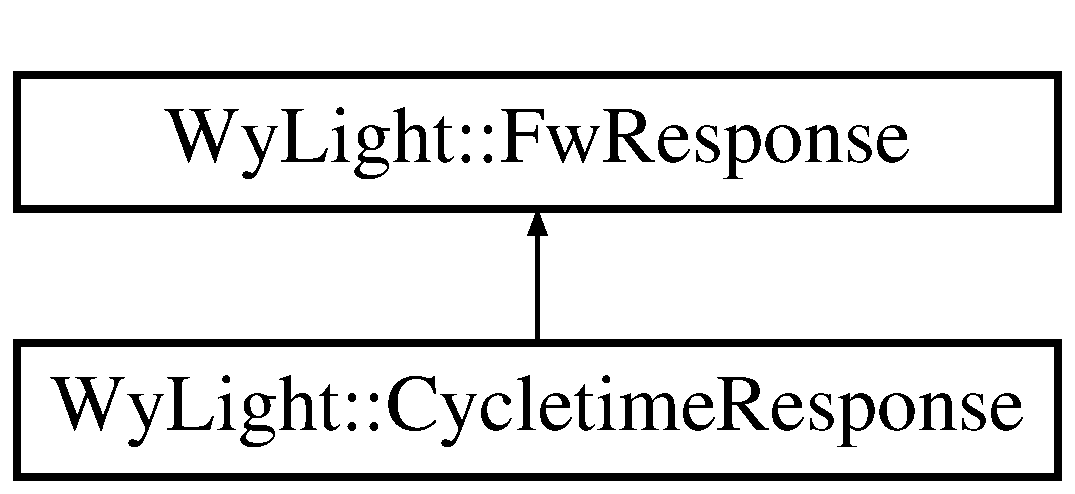
\includegraphics[height=2.000000cm]{class_wy_light_1_1_cycletime_response}
\end{center}
\end{figure}
\subsection*{Public Member Functions}
\begin{DoxyCompactItemize}
\item 
\hyperlink{class_wy_light_1_1_cycletime_response_a188f5503b6ca936497135b764d1d1000}{Cycletime\-Response} (void)
\item 
bool \hyperlink{class_wy_light_1_1_cycletime_response_a44ddaaf66bed8086ad74f15d0c2d6c2a}{Init} (response\-\_\-frame \&p\-Data, size\-\_\-t data\-Length)
\item 
std\-::string \hyperlink{class_wy_light_1_1_cycletime_response_af031ea2856a93586431cda509f85b0f6}{To\-String} (void) const 
\end{DoxyCompactItemize}
\subsection*{Friends}
\begin{DoxyCompactItemize}
\item 
std\-::ostream \& \hyperlink{class_wy_light_1_1_cycletime_response_a297451ca9509cdee481811027a5e31a6}{operator$<$$<$} (std\-::ostream \&out, const \hyperlink{class_wy_light_1_1_cycletime_response}{Cycletime\-Response} \&ref)
\end{DoxyCompactItemize}


\subsection{Constructor \& Destructor Documentation}
\hypertarget{class_wy_light_1_1_cycletime_response_a188f5503b6ca936497135b764d1d1000}{\index{Wy\-Light\-::\-Cycletime\-Response@{Wy\-Light\-::\-Cycletime\-Response}!Cycletime\-Response@{Cycletime\-Response}}
\index{Cycletime\-Response@{Cycletime\-Response}!WyLight::CycletimeResponse@{Wy\-Light\-::\-Cycletime\-Response}}
\subsubsection[{Cycletime\-Response}]{\setlength{\rightskip}{0pt plus 5cm}Wy\-Light\-::\-Cycletime\-Response\-::\-Cycletime\-Response (
\begin{DoxyParamCaption}
\item[{void}]{}
\end{DoxyParamCaption}
)\hspace{0.3cm}{\ttfamily [inline]}}}\label{class_wy_light_1_1_cycletime_response_a188f5503b6ca936497135b764d1d1000}


\subsection{Member Function Documentation}
\hypertarget{class_wy_light_1_1_cycletime_response_a44ddaaf66bed8086ad74f15d0c2d6c2a}{\index{Wy\-Light\-::\-Cycletime\-Response@{Wy\-Light\-::\-Cycletime\-Response}!Init@{Init}}
\index{Init@{Init}!WyLight::CycletimeResponse@{Wy\-Light\-::\-Cycletime\-Response}}
\subsubsection[{Init}]{\setlength{\rightskip}{0pt plus 5cm}bool Wy\-Light\-::\-Cycletime\-Response\-::\-Init (
\begin{DoxyParamCaption}
\item[{response\-\_\-frame \&}]{p\-Data, }
\item[{size\-\_\-t}]{data\-Length}
\end{DoxyParamCaption}
)\hspace{0.3cm}{\ttfamily [inline]}, {\ttfamily [virtual]}}}\label{class_wy_light_1_1_cycletime_response_a44ddaaf66bed8086ad74f15d0c2d6c2a}


Reimplemented from \hyperlink{class_wy_light_1_1_fw_response_aef349b4a6dd0f34c89ed8bcc8c512a55}{Wy\-Light\-::\-Fw\-Response}.

\hypertarget{class_wy_light_1_1_cycletime_response_af031ea2856a93586431cda509f85b0f6}{\index{Wy\-Light\-::\-Cycletime\-Response@{Wy\-Light\-::\-Cycletime\-Response}!To\-String@{To\-String}}
\index{To\-String@{To\-String}!WyLight::CycletimeResponse@{Wy\-Light\-::\-Cycletime\-Response}}
\subsubsection[{To\-String}]{\setlength{\rightskip}{0pt plus 5cm}std\-::string Wy\-Light\-::\-Cycletime\-Response\-::\-To\-String (
\begin{DoxyParamCaption}
\item[{void}]{}
\end{DoxyParamCaption}
) const\hspace{0.3cm}{\ttfamily [inline]}}}\label{class_wy_light_1_1_cycletime_response_af031ea2856a93586431cda509f85b0f6}


\subsection{Friends And Related Function Documentation}
\hypertarget{class_wy_light_1_1_cycletime_response_a297451ca9509cdee481811027a5e31a6}{\index{Wy\-Light\-::\-Cycletime\-Response@{Wy\-Light\-::\-Cycletime\-Response}!operator$<$$<$@{operator$<$$<$}}
\index{operator$<$$<$@{operator$<$$<$}!WyLight::CycletimeResponse@{Wy\-Light\-::\-Cycletime\-Response}}
\subsubsection[{operator$<$$<$}]{\setlength{\rightskip}{0pt plus 5cm}std\-::ostream\& operator$<$$<$ (
\begin{DoxyParamCaption}
\item[{std\-::ostream \&}]{out, }
\item[{const {\bf Cycletime\-Response} \&}]{ref}
\end{DoxyParamCaption}
)\hspace{0.3cm}{\ttfamily [friend]}}}\label{class_wy_light_1_1_cycletime_response_a297451ca9509cdee481811027a5e31a6}


The documentation for this class was generated from the following file\-:\begin{DoxyCompactItemize}
\item 
library/\hyperlink{_fw_response_8h}{Fw\-Response.\-h}\end{DoxyCompactItemize}

\hypertarget{class_wy_light_1_1_endpoint}{\section{Wy\-Light\-:\-:Endpoint Class Reference}
\label{class_wy_light_1_1_endpoint}\index{Wy\-Light\-::\-Endpoint@{Wy\-Light\-::\-Endpoint}}
}


{\ttfamily \#include $<$Endpoint.\-h$>$}

\subsection*{Public Member Functions}
\begin{DoxyCompactItemize}
\item 
\hyperlink{class_wy_light_1_1_endpoint_ab63ad1030b33a946e6874e9a95242652}{Endpoint} (sockaddr\-\_\-storage \&addr, const size\-\_\-t size, uint16\-\_\-t port, std\-::string dev\-Id=\char`\"{}\char`\"{})
\item 
\hyperlink{class_wy_light_1_1_endpoint_ad6953673c9ac61ebbedb32fac5b580ed}{Endpoint} (uint32\-\_\-t ip=0, uint16\-\_\-t port=0, uint8\-\_\-t score=0, std\-::string dev\-Id=\char`\"{}\char`\"{})
\item 
bool \hyperlink{class_wy_light_1_1_endpoint_a23413704ae873962f584e8e4bcb3a3b5}{operator$<$} (const \hyperlink{class_wy_light_1_1_endpoint}{Endpoint} \&ref) const 
\item 
uint64\-\_\-t \hyperlink{class_wy_light_1_1_endpoint_ae0269aa4b78b40366140a4fe98140e67}{As\-Uint64} (void) const 
\item 
std\-::string \hyperlink{class_wy_light_1_1_endpoint_a45f7f0b61014a9732a7c31dec22cfeaf}{Get\-Device\-Id} (void) const 
\item 
uint32\-\_\-t \hyperlink{class_wy_light_1_1_endpoint_a65cca33e7eef5794500621333d2246ed}{Get\-Ip} (void) const 
\item 
uint16\-\_\-t \hyperlink{class_wy_light_1_1_endpoint_ac59441c4d0b60d941150401c118ac63f}{Get\-Port} (void) const 
\item 
uint8\-\_\-t \hyperlink{class_wy_light_1_1_endpoint_a8e19107acfb14d455dde2206b971cc2d}{Get\-Score} (void) const 
\item 
void \hyperlink{class_wy_light_1_1_endpoint_aae5d14042f101187ab51b56dcf217318}{Set\-Device\-Id} (const std\-::string \&device\-Id)
\item 
void \hyperlink{class_wy_light_1_1_endpoint_acab91ff69fc991948b87121e5667b121}{Set\-Score} (const uint8\-\_\-t \&score)
\item 
\hyperlink{class_wy_light_1_1_endpoint}{Endpoint} \& \hyperlink{class_wy_light_1_1_endpoint_a6db37d31aac048566b112e1c25bea7fd}{operator++} (void)
\item 
bool \hyperlink{class_wy_light_1_1_endpoint_a4b0ccfbc29c760fb0c34e9365a3f587d}{Is\-Valid} (void) const 
\end{DoxyCompactItemize}
\subsection*{Friends}
\begin{DoxyCompactItemize}
\item 
std\-::ostream \& \hyperlink{class_wy_light_1_1_endpoint_af3f74b3b812453bb6cc60400dfc0c82c}{operator$<$$<$} (std\-::ostream \&out, const \hyperlink{class_wy_light_1_1_endpoint}{Endpoint} \&ref)
\item 
bool \hyperlink{class_wy_light_1_1_endpoint_a156b06fbd5f39ef344d12405b3dd1dd3}{operator==} (const \hyperlink{class_wy_light_1_1_endpoint}{Endpoint} \&lhs, const \hyperlink{class_wy_light_1_1_endpoint}{Endpoint} \&rhs)
\item 
bool \hyperlink{class_wy_light_1_1_endpoint_a5ae8d57dccffa8396ec6e4a7177a784c}{operator!=} (const \hyperlink{class_wy_light_1_1_endpoint}{Endpoint} \&lhs, const \hyperlink{class_wy_light_1_1_endpoint}{Endpoint} \&rhs)
\end{DoxyCompactItemize}


\subsection{Constructor \& Destructor Documentation}
\hypertarget{class_wy_light_1_1_endpoint_ab63ad1030b33a946e6874e9a95242652}{\index{Wy\-Light\-::\-Endpoint@{Wy\-Light\-::\-Endpoint}!Endpoint@{Endpoint}}
\index{Endpoint@{Endpoint}!WyLight::Endpoint@{Wy\-Light\-::\-Endpoint}}
\subsubsection[{Endpoint}]{\setlength{\rightskip}{0pt plus 5cm}Wy\-Light\-::\-Endpoint\-::\-Endpoint (
\begin{DoxyParamCaption}
\item[{sockaddr\-\_\-storage \&}]{addr, }
\item[{const size\-\_\-t}]{size, }
\item[{uint16\-\_\-t}]{port, }
\item[{std\-::string}]{dev\-Id = {\ttfamily \char`\"{}\char`\"{}}}
\end{DoxyParamCaption}
)\hspace{0.3cm}{\ttfamily [inline]}}}\label{class_wy_light_1_1_endpoint_ab63ad1030b33a946e6874e9a95242652}
\hypertarget{class_wy_light_1_1_endpoint_ad6953673c9ac61ebbedb32fac5b580ed}{\index{Wy\-Light\-::\-Endpoint@{Wy\-Light\-::\-Endpoint}!Endpoint@{Endpoint}}
\index{Endpoint@{Endpoint}!WyLight::Endpoint@{Wy\-Light\-::\-Endpoint}}
\subsubsection[{Endpoint}]{\setlength{\rightskip}{0pt plus 5cm}Wy\-Light\-::\-Endpoint\-::\-Endpoint (
\begin{DoxyParamCaption}
\item[{uint32\-\_\-t}]{ip = {\ttfamily 0}, }
\item[{uint16\-\_\-t}]{port = {\ttfamily 0}, }
\item[{uint8\-\_\-t}]{score = {\ttfamily 0}, }
\item[{std\-::string}]{dev\-Id = {\ttfamily \char`\"{}\char`\"{}}}
\end{DoxyParamCaption}
)\hspace{0.3cm}{\ttfamily [inline]}}}\label{class_wy_light_1_1_endpoint_ad6953673c9ac61ebbedb32fac5b580ed}


\subsection{Member Function Documentation}
\hypertarget{class_wy_light_1_1_endpoint_ae0269aa4b78b40366140a4fe98140e67}{\index{Wy\-Light\-::\-Endpoint@{Wy\-Light\-::\-Endpoint}!As\-Uint64@{As\-Uint64}}
\index{As\-Uint64@{As\-Uint64}!WyLight::Endpoint@{Wy\-Light\-::\-Endpoint}}
\subsubsection[{As\-Uint64}]{\setlength{\rightskip}{0pt plus 5cm}uint64\-\_\-t Wy\-Light\-::\-Endpoint\-::\-As\-Uint64 (
\begin{DoxyParamCaption}
\item[{void}]{}
\end{DoxyParamCaption}
) const\hspace{0.3cm}{\ttfamily [inline]}}}\label{class_wy_light_1_1_endpoint_ae0269aa4b78b40366140a4fe98140e67}
\hypertarget{class_wy_light_1_1_endpoint_a45f7f0b61014a9732a7c31dec22cfeaf}{\index{Wy\-Light\-::\-Endpoint@{Wy\-Light\-::\-Endpoint}!Get\-Device\-Id@{Get\-Device\-Id}}
\index{Get\-Device\-Id@{Get\-Device\-Id}!WyLight::Endpoint@{Wy\-Light\-::\-Endpoint}}
\subsubsection[{Get\-Device\-Id}]{\setlength{\rightskip}{0pt plus 5cm}std\-::string Wy\-Light\-::\-Endpoint\-::\-Get\-Device\-Id (
\begin{DoxyParamCaption}
\item[{void}]{}
\end{DoxyParamCaption}
) const\hspace{0.3cm}{\ttfamily [inline]}}}\label{class_wy_light_1_1_endpoint_a45f7f0b61014a9732a7c31dec22cfeaf}
\hypertarget{class_wy_light_1_1_endpoint_a65cca33e7eef5794500621333d2246ed}{\index{Wy\-Light\-::\-Endpoint@{Wy\-Light\-::\-Endpoint}!Get\-Ip@{Get\-Ip}}
\index{Get\-Ip@{Get\-Ip}!WyLight::Endpoint@{Wy\-Light\-::\-Endpoint}}
\subsubsection[{Get\-Ip}]{\setlength{\rightskip}{0pt plus 5cm}uint32\-\_\-t Wy\-Light\-::\-Endpoint\-::\-Get\-Ip (
\begin{DoxyParamCaption}
\item[{void}]{}
\end{DoxyParamCaption}
) const\hspace{0.3cm}{\ttfamily [inline]}}}\label{class_wy_light_1_1_endpoint_a65cca33e7eef5794500621333d2246ed}
\hypertarget{class_wy_light_1_1_endpoint_ac59441c4d0b60d941150401c118ac63f}{\index{Wy\-Light\-::\-Endpoint@{Wy\-Light\-::\-Endpoint}!Get\-Port@{Get\-Port}}
\index{Get\-Port@{Get\-Port}!WyLight::Endpoint@{Wy\-Light\-::\-Endpoint}}
\subsubsection[{Get\-Port}]{\setlength{\rightskip}{0pt plus 5cm}uint16\-\_\-t Wy\-Light\-::\-Endpoint\-::\-Get\-Port (
\begin{DoxyParamCaption}
\item[{void}]{}
\end{DoxyParamCaption}
) const\hspace{0.3cm}{\ttfamily [inline]}}}\label{class_wy_light_1_1_endpoint_ac59441c4d0b60d941150401c118ac63f}
\hypertarget{class_wy_light_1_1_endpoint_a8e19107acfb14d455dde2206b971cc2d}{\index{Wy\-Light\-::\-Endpoint@{Wy\-Light\-::\-Endpoint}!Get\-Score@{Get\-Score}}
\index{Get\-Score@{Get\-Score}!WyLight::Endpoint@{Wy\-Light\-::\-Endpoint}}
\subsubsection[{Get\-Score}]{\setlength{\rightskip}{0pt plus 5cm}uint8\-\_\-t Wy\-Light\-::\-Endpoint\-::\-Get\-Score (
\begin{DoxyParamCaption}
\item[{void}]{}
\end{DoxyParamCaption}
) const\hspace{0.3cm}{\ttfamily [inline]}}}\label{class_wy_light_1_1_endpoint_a8e19107acfb14d455dde2206b971cc2d}
\hypertarget{class_wy_light_1_1_endpoint_a4b0ccfbc29c760fb0c34e9365a3f587d}{\index{Wy\-Light\-::\-Endpoint@{Wy\-Light\-::\-Endpoint}!Is\-Valid@{Is\-Valid}}
\index{Is\-Valid@{Is\-Valid}!WyLight::Endpoint@{Wy\-Light\-::\-Endpoint}}
\subsubsection[{Is\-Valid}]{\setlength{\rightskip}{0pt plus 5cm}bool Wy\-Light\-::\-Endpoint\-::\-Is\-Valid (
\begin{DoxyParamCaption}
\item[{void}]{}
\end{DoxyParamCaption}
) const\hspace{0.3cm}{\ttfamily [inline]}}}\label{class_wy_light_1_1_endpoint_a4b0ccfbc29c760fb0c34e9365a3f587d}
\hypertarget{class_wy_light_1_1_endpoint_a6db37d31aac048566b112e1c25bea7fd}{\index{Wy\-Light\-::\-Endpoint@{Wy\-Light\-::\-Endpoint}!operator++@{operator++}}
\index{operator++@{operator++}!WyLight::Endpoint@{Wy\-Light\-::\-Endpoint}}
\subsubsection[{operator++}]{\setlength{\rightskip}{0pt plus 5cm}{\bf Endpoint}\& Wy\-Light\-::\-Endpoint\-::operator++ (
\begin{DoxyParamCaption}
\item[{void}]{}
\end{DoxyParamCaption}
)\hspace{0.3cm}{\ttfamily [inline]}}}\label{class_wy_light_1_1_endpoint_a6db37d31aac048566b112e1c25bea7fd}
\hypertarget{class_wy_light_1_1_endpoint_a23413704ae873962f584e8e4bcb3a3b5}{\index{Wy\-Light\-::\-Endpoint@{Wy\-Light\-::\-Endpoint}!operator$<$@{operator$<$}}
\index{operator$<$@{operator$<$}!WyLight::Endpoint@{Wy\-Light\-::\-Endpoint}}
\subsubsection[{operator$<$}]{\setlength{\rightskip}{0pt plus 5cm}bool Wy\-Light\-::\-Endpoint\-::operator$<$ (
\begin{DoxyParamCaption}
\item[{const {\bf Endpoint} \&}]{ref}
\end{DoxyParamCaption}
) const\hspace{0.3cm}{\ttfamily [inline]}}}\label{class_wy_light_1_1_endpoint_a23413704ae873962f584e8e4bcb3a3b5}
\hypertarget{class_wy_light_1_1_endpoint_aae5d14042f101187ab51b56dcf217318}{\index{Wy\-Light\-::\-Endpoint@{Wy\-Light\-::\-Endpoint}!Set\-Device\-Id@{Set\-Device\-Id}}
\index{Set\-Device\-Id@{Set\-Device\-Id}!WyLight::Endpoint@{Wy\-Light\-::\-Endpoint}}
\subsubsection[{Set\-Device\-Id}]{\setlength{\rightskip}{0pt plus 5cm}void Wy\-Light\-::\-Endpoint\-::\-Set\-Device\-Id (
\begin{DoxyParamCaption}
\item[{const std\-::string \&}]{device\-Id}
\end{DoxyParamCaption}
)\hspace{0.3cm}{\ttfamily [inline]}}}\label{class_wy_light_1_1_endpoint_aae5d14042f101187ab51b56dcf217318}
\hypertarget{class_wy_light_1_1_endpoint_acab91ff69fc991948b87121e5667b121}{\index{Wy\-Light\-::\-Endpoint@{Wy\-Light\-::\-Endpoint}!Set\-Score@{Set\-Score}}
\index{Set\-Score@{Set\-Score}!WyLight::Endpoint@{Wy\-Light\-::\-Endpoint}}
\subsubsection[{Set\-Score}]{\setlength{\rightskip}{0pt plus 5cm}void Wy\-Light\-::\-Endpoint\-::\-Set\-Score (
\begin{DoxyParamCaption}
\item[{const uint8\-\_\-t \&}]{score}
\end{DoxyParamCaption}
)\hspace{0.3cm}{\ttfamily [inline]}}}\label{class_wy_light_1_1_endpoint_acab91ff69fc991948b87121e5667b121}


\subsection{Friends And Related Function Documentation}
\hypertarget{class_wy_light_1_1_endpoint_a5ae8d57dccffa8396ec6e4a7177a784c}{\index{Wy\-Light\-::\-Endpoint@{Wy\-Light\-::\-Endpoint}!operator!=@{operator!=}}
\index{operator!=@{operator!=}!WyLight::Endpoint@{Wy\-Light\-::\-Endpoint}}
\subsubsection[{operator!=}]{\setlength{\rightskip}{0pt plus 5cm}bool operator!= (
\begin{DoxyParamCaption}
\item[{const {\bf Endpoint} \&}]{lhs, }
\item[{const {\bf Endpoint} \&}]{rhs}
\end{DoxyParamCaption}
)\hspace{0.3cm}{\ttfamily [friend]}}}\label{class_wy_light_1_1_endpoint_a5ae8d57dccffa8396ec6e4a7177a784c}
\hypertarget{class_wy_light_1_1_endpoint_af3f74b3b812453bb6cc60400dfc0c82c}{\index{Wy\-Light\-::\-Endpoint@{Wy\-Light\-::\-Endpoint}!operator$<$$<$@{operator$<$$<$}}
\index{operator$<$$<$@{operator$<$$<$}!WyLight::Endpoint@{Wy\-Light\-::\-Endpoint}}
\subsubsection[{operator$<$$<$}]{\setlength{\rightskip}{0pt plus 5cm}std\-::ostream\& operator$<$$<$ (
\begin{DoxyParamCaption}
\item[{std\-::ostream \&}]{out, }
\item[{const {\bf Endpoint} \&}]{ref}
\end{DoxyParamCaption}
)\hspace{0.3cm}{\ttfamily [friend]}}}\label{class_wy_light_1_1_endpoint_af3f74b3b812453bb6cc60400dfc0c82c}
\hypertarget{class_wy_light_1_1_endpoint_a156b06fbd5f39ef344d12405b3dd1dd3}{\index{Wy\-Light\-::\-Endpoint@{Wy\-Light\-::\-Endpoint}!operator==@{operator==}}
\index{operator==@{operator==}!WyLight::Endpoint@{Wy\-Light\-::\-Endpoint}}
\subsubsection[{operator==}]{\setlength{\rightskip}{0pt plus 5cm}bool operator== (
\begin{DoxyParamCaption}
\item[{const {\bf Endpoint} \&}]{lhs, }
\item[{const {\bf Endpoint} \&}]{rhs}
\end{DoxyParamCaption}
)\hspace{0.3cm}{\ttfamily [friend]}}}\label{class_wy_light_1_1_endpoint_a156b06fbd5f39ef344d12405b3dd1dd3}


The documentation for this class was generated from the following file\-:\begin{DoxyCompactItemize}
\item 
library/\hyperlink{_endpoint_8h}{Endpoint.\-h}\end{DoxyCompactItemize}

\hypertarget{class_wy_light_1_1_fatal_error}{\section{Wy\-Light\-:\-:Fatal\-Error Class Reference}
\label{class_wy_light_1_1_fatal_error}\index{Wy\-Light\-::\-Fatal\-Error@{Wy\-Light\-::\-Fatal\-Error}}
}


{\ttfamily \#include $<$Wifly\-Control\-Exception.\-h$>$}

Inheritance diagram for Wy\-Light\-:\-:Fatal\-Error\-:\begin{figure}[H]
\begin{center}
\leavevmode
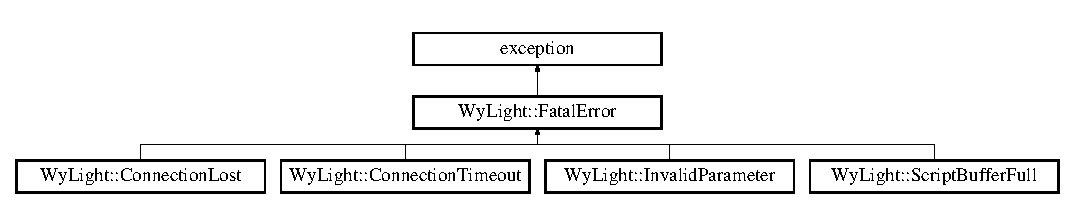
\includegraphics[height=2.359551cm]{class_wy_light_1_1_fatal_error}
\end{center}
\end{figure}
\subsection*{Public Member Functions}
\begin{DoxyCompactItemize}
\item 
\hyperlink{class_wy_light_1_1_fatal_error_ab9aa2dc0e064e47d56052e0e9084200f}{Fatal\-Error} (const std\-::string \&description, uint32\-\_\-t error\-Code=\hyperlink{namespace_wy_light_afd625f917b07e9c48f67c4383af5773fab15784bfc61f7544f4b3bbac1817a793}{F\-A\-T\-A\-L\-\_\-\-E\-R\-R\-O\-R})  throw ()
\item 
virtual \hyperlink{class_wy_light_1_1_fatal_error_ae76658416075b597f03bee95f21f7a96}{$\sim$\-Fatal\-Error} (void)  throw ()
\item 
uint32\-\_\-t \hyperlink{class_wy_light_1_1_fatal_error_a15ae0113906c71cf34d631767371042c}{As\-Error\-Code} (void) const 
\item 
virtual const char $\ast$ \hyperlink{class_wy_light_1_1_fatal_error_aa74decc09fe8aafc15bfbe31f697987a}{Get\-Java\-Class\-Type} (void) const 
\item 
const char $\ast$ \hyperlink{class_wy_light_1_1_fatal_error_a971784e107b804fa177788061594a47d}{what} (void) const   throw ()
\end{DoxyCompactItemize}
\subsection*{Protected Attributes}
\begin{DoxyCompactItemize}
\item 
const std\-::string \hyperlink{class_wy_light_1_1_fatal_error_aeae1bd38ee1c9b21b260a10ecc89b5f4}{m\-Description}
\item 
const uint32\-\_\-t \hyperlink{class_wy_light_1_1_fatal_error_a7d6df57841d017b51107a80ac6205c93}{m\-Error\-Code}
\end{DoxyCompactItemize}
\subsection*{Friends}
\begin{DoxyCompactItemize}
\item 
std\-::ostream \& \hyperlink{class_wy_light_1_1_fatal_error_ae2c3ada9625867398d5bbd51b1223a13}{operator$<$$<$} (std\-::ostream \&out, const \hyperlink{class_wy_light_1_1_fatal_error}{Fatal\-Error} \&ref)
\end{DoxyCompactItemize}


\subsection{Constructor \& Destructor Documentation}
\hypertarget{class_wy_light_1_1_fatal_error_ab9aa2dc0e064e47d56052e0e9084200f}{\index{Wy\-Light\-::\-Fatal\-Error@{Wy\-Light\-::\-Fatal\-Error}!Fatal\-Error@{Fatal\-Error}}
\index{Fatal\-Error@{Fatal\-Error}!WyLight::FatalError@{Wy\-Light\-::\-Fatal\-Error}}
\subsubsection[{Fatal\-Error}]{\setlength{\rightskip}{0pt plus 5cm}Wy\-Light\-::\-Fatal\-Error\-::\-Fatal\-Error (
\begin{DoxyParamCaption}
\item[{const std\-::string \&}]{description, }
\item[{uint32\-\_\-t}]{error\-Code = {\ttfamily {\bf F\-A\-T\-A\-L\-\_\-\-E\-R\-R\-O\-R}}}
\end{DoxyParamCaption}
)  throw ()\hspace{0.3cm}{\ttfamily [inline]}}}\label{class_wy_light_1_1_fatal_error_ab9aa2dc0e064e47d56052e0e9084200f}
\hypertarget{class_wy_light_1_1_fatal_error_ae76658416075b597f03bee95f21f7a96}{\index{Wy\-Light\-::\-Fatal\-Error@{Wy\-Light\-::\-Fatal\-Error}!$\sim$\-Fatal\-Error@{$\sim$\-Fatal\-Error}}
\index{$\sim$\-Fatal\-Error@{$\sim$\-Fatal\-Error}!WyLight::FatalError@{Wy\-Light\-::\-Fatal\-Error}}
\subsubsection[{$\sim$\-Fatal\-Error}]{\setlength{\rightskip}{0pt plus 5cm}virtual Wy\-Light\-::\-Fatal\-Error\-::$\sim$\-Fatal\-Error (
\begin{DoxyParamCaption}
\item[{void}]{}
\end{DoxyParamCaption}
)  throw ()\hspace{0.3cm}{\ttfamily [inline]}, {\ttfamily [virtual]}}}\label{class_wy_light_1_1_fatal_error_ae76658416075b597f03bee95f21f7a96}


\subsection{Member Function Documentation}
\hypertarget{class_wy_light_1_1_fatal_error_a15ae0113906c71cf34d631767371042c}{\index{Wy\-Light\-::\-Fatal\-Error@{Wy\-Light\-::\-Fatal\-Error}!As\-Error\-Code@{As\-Error\-Code}}
\index{As\-Error\-Code@{As\-Error\-Code}!WyLight::FatalError@{Wy\-Light\-::\-Fatal\-Error}}
\subsubsection[{As\-Error\-Code}]{\setlength{\rightskip}{0pt plus 5cm}uint32\-\_\-t Wy\-Light\-::\-Fatal\-Error\-::\-As\-Error\-Code (
\begin{DoxyParamCaption}
\item[{void}]{}
\end{DoxyParamCaption}
) const\hspace{0.3cm}{\ttfamily [inline]}}}\label{class_wy_light_1_1_fatal_error_a15ae0113906c71cf34d631767371042c}
\hypertarget{class_wy_light_1_1_fatal_error_aa74decc09fe8aafc15bfbe31f697987a}{\index{Wy\-Light\-::\-Fatal\-Error@{Wy\-Light\-::\-Fatal\-Error}!Get\-Java\-Class\-Type@{Get\-Java\-Class\-Type}}
\index{Get\-Java\-Class\-Type@{Get\-Java\-Class\-Type}!WyLight::FatalError@{Wy\-Light\-::\-Fatal\-Error}}
\subsubsection[{Get\-Java\-Class\-Type}]{\setlength{\rightskip}{0pt plus 5cm}virtual const char$\ast$ Wy\-Light\-::\-Fatal\-Error\-::\-Get\-Java\-Class\-Type (
\begin{DoxyParamCaption}
\item[{void}]{}
\end{DoxyParamCaption}
) const\hspace{0.3cm}{\ttfamily [inline]}, {\ttfamily [virtual]}}}\label{class_wy_light_1_1_fatal_error_aa74decc09fe8aafc15bfbe31f697987a}


Reimplemented in \hyperlink{class_wy_light_1_1_script_buffer_full_ac228a7696643e89e4a571347bc9dda7d}{Wy\-Light\-::\-Script\-Buffer\-Full}, \hyperlink{class_wy_light_1_1_invalid_parameter_a3cfc3b57f7a18e051e72efcfb4a67deb}{Wy\-Light\-::\-Invalid\-Parameter}, \hyperlink{class_wy_light_1_1_connection_timeout_a2feb264902a3c11a10f4e9eb1ba08bb1}{Wy\-Light\-::\-Connection\-Timeout}, and \hyperlink{class_wy_light_1_1_connection_lost_a32dbb008e84c419fdb31b7b4b13b6f7f}{Wy\-Light\-::\-Connection\-Lost}.

\hypertarget{class_wy_light_1_1_fatal_error_a971784e107b804fa177788061594a47d}{\index{Wy\-Light\-::\-Fatal\-Error@{Wy\-Light\-::\-Fatal\-Error}!what@{what}}
\index{what@{what}!WyLight::FatalError@{Wy\-Light\-::\-Fatal\-Error}}
\subsubsection[{what}]{\setlength{\rightskip}{0pt plus 5cm}const char$\ast$ Wy\-Light\-::\-Fatal\-Error\-::what (
\begin{DoxyParamCaption}
\item[{void}]{}
\end{DoxyParamCaption}
) const  throw ()\hspace{0.3cm}{\ttfamily [inline]}}}\label{class_wy_light_1_1_fatal_error_a971784e107b804fa177788061594a47d}


\subsection{Friends And Related Function Documentation}
\hypertarget{class_wy_light_1_1_fatal_error_ae2c3ada9625867398d5bbd51b1223a13}{\index{Wy\-Light\-::\-Fatal\-Error@{Wy\-Light\-::\-Fatal\-Error}!operator$<$$<$@{operator$<$$<$}}
\index{operator$<$$<$@{operator$<$$<$}!WyLight::FatalError@{Wy\-Light\-::\-Fatal\-Error}}
\subsubsection[{operator$<$$<$}]{\setlength{\rightskip}{0pt plus 5cm}std\-::ostream\& operator$<$$<$ (
\begin{DoxyParamCaption}
\item[{std\-::ostream \&}]{out, }
\item[{const {\bf Fatal\-Error} \&}]{ref}
\end{DoxyParamCaption}
)\hspace{0.3cm}{\ttfamily [friend]}}}\label{class_wy_light_1_1_fatal_error_ae2c3ada9625867398d5bbd51b1223a13}


\subsection{Member Data Documentation}
\hypertarget{class_wy_light_1_1_fatal_error_aeae1bd38ee1c9b21b260a10ecc89b5f4}{\index{Wy\-Light\-::\-Fatal\-Error@{Wy\-Light\-::\-Fatal\-Error}!m\-Description@{m\-Description}}
\index{m\-Description@{m\-Description}!WyLight::FatalError@{Wy\-Light\-::\-Fatal\-Error}}
\subsubsection[{m\-Description}]{\setlength{\rightskip}{0pt plus 5cm}const std\-::string Wy\-Light\-::\-Fatal\-Error\-::m\-Description\hspace{0.3cm}{\ttfamily [protected]}}}\label{class_wy_light_1_1_fatal_error_aeae1bd38ee1c9b21b260a10ecc89b5f4}
\hypertarget{class_wy_light_1_1_fatal_error_a7d6df57841d017b51107a80ac6205c93}{\index{Wy\-Light\-::\-Fatal\-Error@{Wy\-Light\-::\-Fatal\-Error}!m\-Error\-Code@{m\-Error\-Code}}
\index{m\-Error\-Code@{m\-Error\-Code}!WyLight::FatalError@{Wy\-Light\-::\-Fatal\-Error}}
\subsubsection[{m\-Error\-Code}]{\setlength{\rightskip}{0pt plus 5cm}const uint32\-\_\-t Wy\-Light\-::\-Fatal\-Error\-::m\-Error\-Code\hspace{0.3cm}{\ttfamily [protected]}}}\label{class_wy_light_1_1_fatal_error_a7d6df57841d017b51107a80ac6205c93}


The documentation for this class was generated from the following file\-:\begin{DoxyCompactItemize}
\item 
library/\hyperlink{_wifly_control_exception_8h}{Wifly\-Control\-Exception.\-h}\end{DoxyCompactItemize}

\hypertarget{class_wy_light_1_1_firmware_version_response}{\section{Wy\-Light\-:\-:Firmware\-Version\-Response Class Reference}
\label{class_wy_light_1_1_firmware_version_response}\index{Wy\-Light\-::\-Firmware\-Version\-Response@{Wy\-Light\-::\-Firmware\-Version\-Response}}
}


{\ttfamily \#include $<$Fw\-Response.\-h$>$}

Inheritance diagram for Wy\-Light\-:\-:Firmware\-Version\-Response\-:\begin{figure}[H]
\begin{center}
\leavevmode
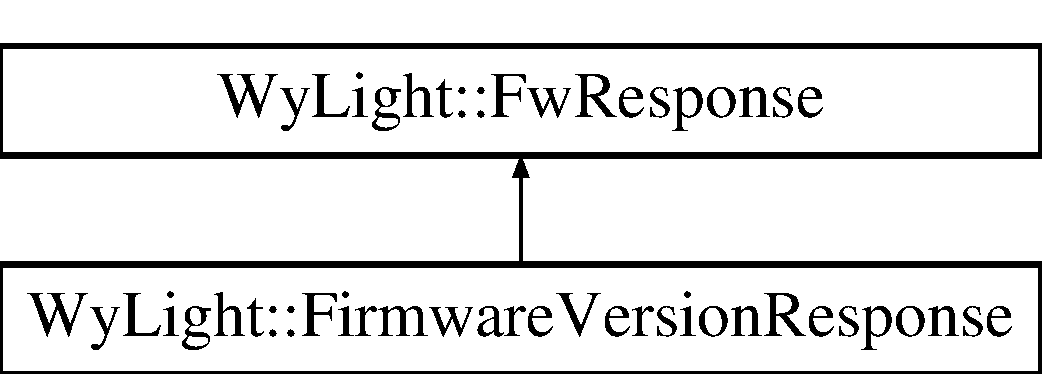
\includegraphics[height=2.000000cm]{class_wy_light_1_1_firmware_version_response}
\end{center}
\end{figure}
\subsection*{Public Member Functions}
\begin{DoxyCompactItemize}
\item 
\hyperlink{class_wy_light_1_1_firmware_version_response_ac44161f34f697b6603248eb334e37330}{Firmware\-Version\-Response} (void)
\item 
bool \hyperlink{class_wy_light_1_1_firmware_version_response_ada5e917af8c5f256a11418fe5ba51211}{Init} (response\-\_\-frame \&p\-Data, size\-\_\-t data\-Length)
\item 
std\-::string \hyperlink{class_wy_light_1_1_firmware_version_response_a1c783d24e4ba46201d414664c4c33506}{To\-String} (void) const 
\end{DoxyCompactItemize}
\subsection*{Friends}
\begin{DoxyCompactItemize}
\item 
std\-::ostream \& \hyperlink{class_wy_light_1_1_firmware_version_response_a37b570544d9c72195251b87e598a0451}{operator$<$$<$} (std\-::ostream \&out, const \hyperlink{class_wy_light_1_1_firmware_version_response}{Firmware\-Version\-Response} \&ref)
\end{DoxyCompactItemize}


\subsection{Constructor \& Destructor Documentation}
\hypertarget{class_wy_light_1_1_firmware_version_response_ac44161f34f697b6603248eb334e37330}{\index{Wy\-Light\-::\-Firmware\-Version\-Response@{Wy\-Light\-::\-Firmware\-Version\-Response}!Firmware\-Version\-Response@{Firmware\-Version\-Response}}
\index{Firmware\-Version\-Response@{Firmware\-Version\-Response}!WyLight::FirmwareVersionResponse@{Wy\-Light\-::\-Firmware\-Version\-Response}}
\subsubsection[{Firmware\-Version\-Response}]{\setlength{\rightskip}{0pt plus 5cm}Wy\-Light\-::\-Firmware\-Version\-Response\-::\-Firmware\-Version\-Response (
\begin{DoxyParamCaption}
\item[{void}]{}
\end{DoxyParamCaption}
)\hspace{0.3cm}{\ttfamily [inline]}}}\label{class_wy_light_1_1_firmware_version_response_ac44161f34f697b6603248eb334e37330}


\subsection{Member Function Documentation}
\hypertarget{class_wy_light_1_1_firmware_version_response_ada5e917af8c5f256a11418fe5ba51211}{\index{Wy\-Light\-::\-Firmware\-Version\-Response@{Wy\-Light\-::\-Firmware\-Version\-Response}!Init@{Init}}
\index{Init@{Init}!WyLight::FirmwareVersionResponse@{Wy\-Light\-::\-Firmware\-Version\-Response}}
\subsubsection[{Init}]{\setlength{\rightskip}{0pt plus 5cm}bool Wy\-Light\-::\-Firmware\-Version\-Response\-::\-Init (
\begin{DoxyParamCaption}
\item[{response\-\_\-frame \&}]{p\-Data, }
\item[{size\-\_\-t}]{data\-Length}
\end{DoxyParamCaption}
)\hspace{0.3cm}{\ttfamily [inline]}, {\ttfamily [virtual]}}}\label{class_wy_light_1_1_firmware_version_response_ada5e917af8c5f256a11418fe5ba51211}


Reimplemented from \hyperlink{class_wy_light_1_1_fw_response_aef349b4a6dd0f34c89ed8bcc8c512a55}{Wy\-Light\-::\-Fw\-Response}.

\hypertarget{class_wy_light_1_1_firmware_version_response_a1c783d24e4ba46201d414664c4c33506}{\index{Wy\-Light\-::\-Firmware\-Version\-Response@{Wy\-Light\-::\-Firmware\-Version\-Response}!To\-String@{To\-String}}
\index{To\-String@{To\-String}!WyLight::FirmwareVersionResponse@{Wy\-Light\-::\-Firmware\-Version\-Response}}
\subsubsection[{To\-String}]{\setlength{\rightskip}{0pt plus 5cm}std\-::string Wy\-Light\-::\-Firmware\-Version\-Response\-::\-To\-String (
\begin{DoxyParamCaption}
\item[{void}]{}
\end{DoxyParamCaption}
) const\hspace{0.3cm}{\ttfamily [inline]}}}\label{class_wy_light_1_1_firmware_version_response_a1c783d24e4ba46201d414664c4c33506}


\subsection{Friends And Related Function Documentation}
\hypertarget{class_wy_light_1_1_firmware_version_response_a37b570544d9c72195251b87e598a0451}{\index{Wy\-Light\-::\-Firmware\-Version\-Response@{Wy\-Light\-::\-Firmware\-Version\-Response}!operator$<$$<$@{operator$<$$<$}}
\index{operator$<$$<$@{operator$<$$<$}!WyLight::FirmwareVersionResponse@{Wy\-Light\-::\-Firmware\-Version\-Response}}
\subsubsection[{operator$<$$<$}]{\setlength{\rightskip}{0pt plus 5cm}std\-::ostream\& operator$<$$<$ (
\begin{DoxyParamCaption}
\item[{std\-::ostream \&}]{out, }
\item[{const {\bf Firmware\-Version\-Response} \&}]{ref}
\end{DoxyParamCaption}
)\hspace{0.3cm}{\ttfamily [friend]}}}\label{class_wy_light_1_1_firmware_version_response_a37b570544d9c72195251b87e598a0451}


The documentation for this class was generated from the following file\-:\begin{DoxyCompactItemize}
\item 
library/\hyperlink{_fw_response_8h}{Fw\-Response.\-h}\end{DoxyCompactItemize}

\hypertarget{struct_wy_light_1_1_fw_cmd_clear_script}{\section{Wy\-Light\-:\-:Fw\-Cmd\-Clear\-Script Struct Reference}
\label{struct_wy_light_1_1_fw_cmd_clear_script}\index{Wy\-Light\-::\-Fw\-Cmd\-Clear\-Script@{Wy\-Light\-::\-Fw\-Cmd\-Clear\-Script}}
}


{\ttfamily \#include $<$Fw\-Command.\-h$>$}

Inheritance diagram for Wy\-Light\-:\-:Fw\-Cmd\-Clear\-Script\-:\begin{figure}[H]
\begin{center}
\leavevmode
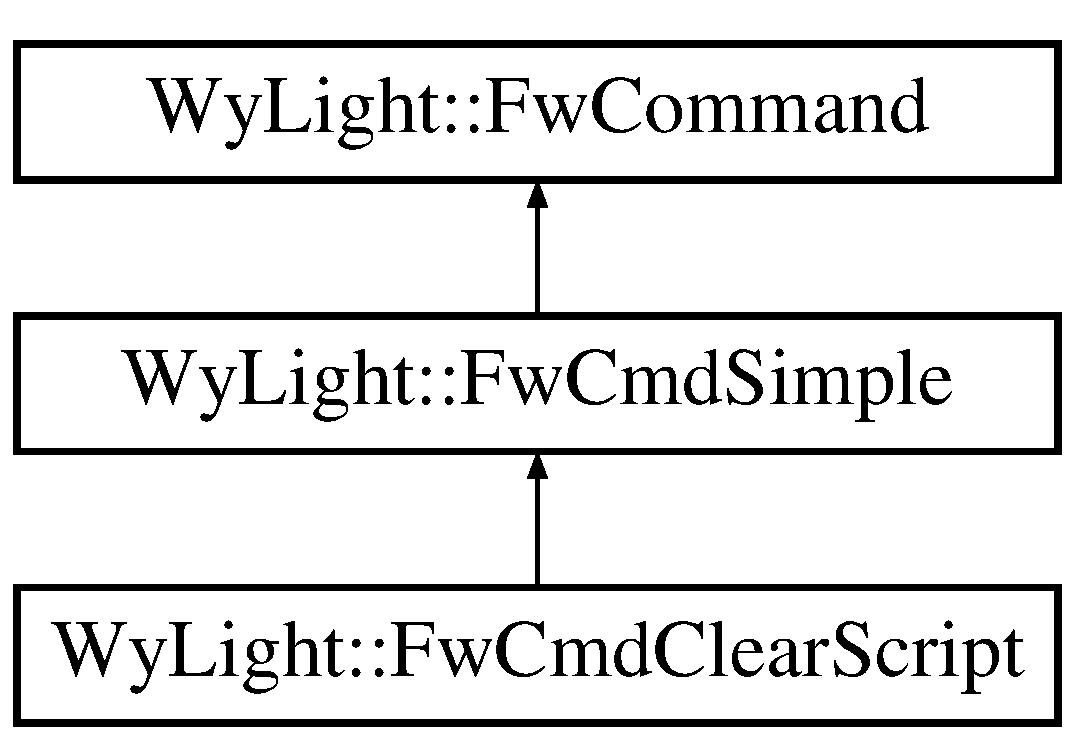
\includegraphics[height=3.000000cm]{struct_wy_light_1_1_fw_cmd_clear_script}
\end{center}
\end{figure}
\subsection*{Public Member Functions}
\begin{DoxyCompactItemize}
\item 
\hyperlink{struct_wy_light_1_1_fw_cmd_clear_script_a215e609e9fb110bb9f41f015ffb8f87d}{Fw\-Cmd\-Clear\-Script} (void)
\end{DoxyCompactItemize}
\subsection*{Additional Inherited Members}


\subsection{Detailed Description}
Wipe all commands from the \hyperlink{namespace_wy_light}{Wy\-Light} script controller 

\subsection{Constructor \& Destructor Documentation}
\hypertarget{struct_wy_light_1_1_fw_cmd_clear_script_a215e609e9fb110bb9f41f015ffb8f87d}{\index{Wy\-Light\-::\-Fw\-Cmd\-Clear\-Script@{Wy\-Light\-::\-Fw\-Cmd\-Clear\-Script}!Fw\-Cmd\-Clear\-Script@{Fw\-Cmd\-Clear\-Script}}
\index{Fw\-Cmd\-Clear\-Script@{Fw\-Cmd\-Clear\-Script}!WyLight::FwCmdClearScript@{Wy\-Light\-::\-Fw\-Cmd\-Clear\-Script}}
\subsubsection[{Fw\-Cmd\-Clear\-Script}]{\setlength{\rightskip}{0pt plus 5cm}Wy\-Light\-::\-Fw\-Cmd\-Clear\-Script\-::\-Fw\-Cmd\-Clear\-Script (
\begin{DoxyParamCaption}
\item[{void}]{}
\end{DoxyParamCaption}
)\hspace{0.3cm}{\ttfamily [inline]}}}\label{struct_wy_light_1_1_fw_cmd_clear_script_a215e609e9fb110bb9f41f015ffb8f87d}


The documentation for this struct was generated from the following file\-:\begin{DoxyCompactItemize}
\item 
library/\hyperlink{_fw_command_8h}{Fw\-Command.\-h}\end{DoxyCompactItemize}

\hypertarget{struct_wy_light_1_1_fw_cmd_get}{\section{Wy\-Light\-:\-:Fw\-Cmd\-Get Struct Reference}
\label{struct_wy_light_1_1_fw_cmd_get}\index{Wy\-Light\-::\-Fw\-Cmd\-Get@{Wy\-Light\-::\-Fw\-Cmd\-Get}}
}


{\ttfamily \#include $<$Fw\-Command.\-h$>$}

Inheritance diagram for Wy\-Light\-:\-:Fw\-Cmd\-Get\-:\begin{figure}[H]
\begin{center}
\leavevmode
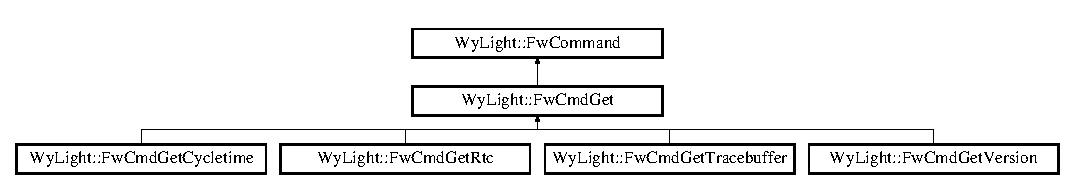
\includegraphics[height=2.110553cm]{struct_wy_light_1_1_fw_cmd_get}
\end{center}
\end{figure}
\subsection*{Public Member Functions}
\begin{DoxyCompactItemize}
\item 
\hyperlink{struct_wy_light_1_1_fw_cmd_get_a1a04aece1d971a7867b0b739dbb61ec2}{Fw\-Cmd\-Get} (uint8\-\_\-t cmd)
\end{DoxyCompactItemize}
\subsection*{Additional Inherited Members}


\subsection{Constructor \& Destructor Documentation}
\hypertarget{struct_wy_light_1_1_fw_cmd_get_a1a04aece1d971a7867b0b739dbb61ec2}{\index{Wy\-Light\-::\-Fw\-Cmd\-Get@{Wy\-Light\-::\-Fw\-Cmd\-Get}!Fw\-Cmd\-Get@{Fw\-Cmd\-Get}}
\index{Fw\-Cmd\-Get@{Fw\-Cmd\-Get}!WyLight::FwCmdGet@{Wy\-Light\-::\-Fw\-Cmd\-Get}}
\subsubsection[{Fw\-Cmd\-Get}]{\setlength{\rightskip}{0pt plus 5cm}Wy\-Light\-::\-Fw\-Cmd\-Get\-::\-Fw\-Cmd\-Get (
\begin{DoxyParamCaption}
\item[{uint8\-\_\-t}]{cmd}
\end{DoxyParamCaption}
)\hspace{0.3cm}{\ttfamily [inline]}}}\label{struct_wy_light_1_1_fw_cmd_get_a1a04aece1d971a7867b0b739dbb61ec2}


The documentation for this struct was generated from the following file\-:\begin{DoxyCompactItemize}
\item 
library/\hyperlink{_fw_command_8h}{Fw\-Command.\-h}\end{DoxyCompactItemize}

\hypertarget{struct_wy_light_1_1_fw_cmd_get_cycletime}{\section{Wy\-Light\-:\-:Fw\-Cmd\-Get\-Cycletime Struct Reference}
\label{struct_wy_light_1_1_fw_cmd_get_cycletime}\index{Wy\-Light\-::\-Fw\-Cmd\-Get\-Cycletime@{Wy\-Light\-::\-Fw\-Cmd\-Get\-Cycletime}}
}


{\ttfamily \#include $<$Fw\-Command.\-h$>$}

Inheritance diagram for Wy\-Light\-:\-:Fw\-Cmd\-Get\-Cycletime\-:\begin{figure}[H]
\begin{center}
\leavevmode
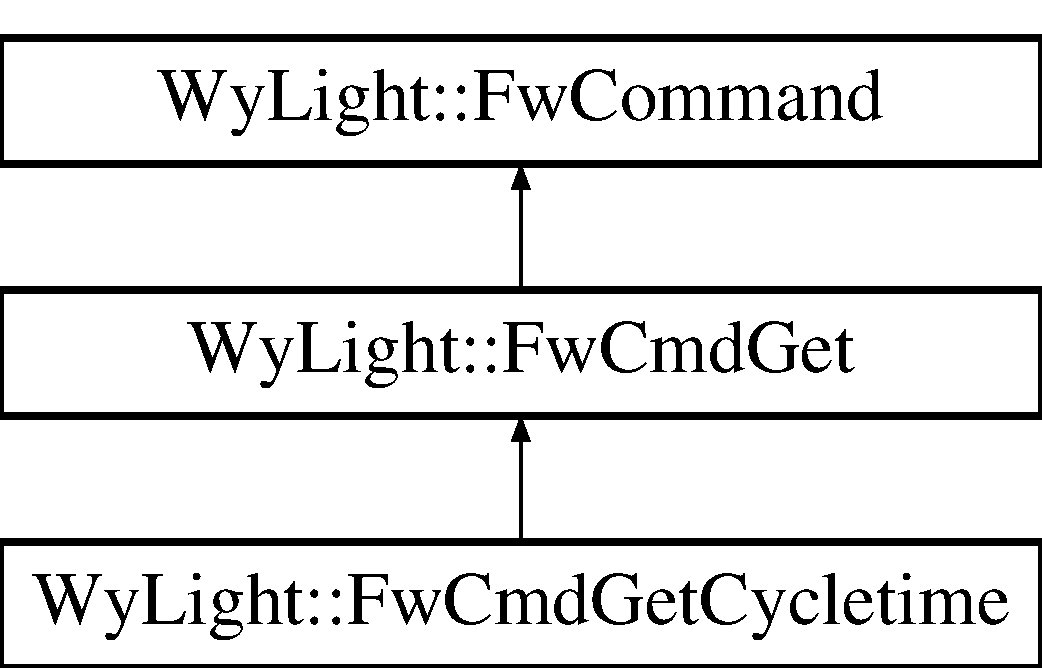
\includegraphics[height=3.000000cm]{struct_wy_light_1_1_fw_cmd_get_cycletime}
\end{center}
\end{figure}
\subsection*{Public Member Functions}
\begin{DoxyCompactItemize}
\item 
\hyperlink{struct_wy_light_1_1_fw_cmd_get_cycletime_a3ef62336a758f30f4e9c07cff7907b97}{Fw\-Cmd\-Get\-Cycletime} (void)
\item 
\hyperlink{class_wy_light_1_1_fw_response}{Fw\-Response} \& \hyperlink{struct_wy_light_1_1_fw_cmd_get_cycletime_aa6b457bdab92b36b2e16f88868e78beb}{Get\-Response} (void)
\end{DoxyCompactItemize}
\subsection*{Public Attributes}
\begin{DoxyCompactItemize}
\item 
\hyperlink{class_wy_light_1_1_cycletime_response}{Cycletime\-Response} \hyperlink{struct_wy_light_1_1_fw_cmd_get_cycletime_aee08eb755ea6f308d9ce9cd78adc9517}{m\-Response}
\end{DoxyCompactItemize}
\subsection*{Additional Inherited Members}


\subsection{Constructor \& Destructor Documentation}
\hypertarget{struct_wy_light_1_1_fw_cmd_get_cycletime_a3ef62336a758f30f4e9c07cff7907b97}{\index{Wy\-Light\-::\-Fw\-Cmd\-Get\-Cycletime@{Wy\-Light\-::\-Fw\-Cmd\-Get\-Cycletime}!Fw\-Cmd\-Get\-Cycletime@{Fw\-Cmd\-Get\-Cycletime}}
\index{Fw\-Cmd\-Get\-Cycletime@{Fw\-Cmd\-Get\-Cycletime}!WyLight::FwCmdGetCycletime@{Wy\-Light\-::\-Fw\-Cmd\-Get\-Cycletime}}
\subsubsection[{Fw\-Cmd\-Get\-Cycletime}]{\setlength{\rightskip}{0pt plus 5cm}Wy\-Light\-::\-Fw\-Cmd\-Get\-Cycletime\-::\-Fw\-Cmd\-Get\-Cycletime (
\begin{DoxyParamCaption}
\item[{void}]{}
\end{DoxyParamCaption}
)\hspace{0.3cm}{\ttfamily [inline]}}}\label{struct_wy_light_1_1_fw_cmd_get_cycletime_a3ef62336a758f30f4e9c07cff7907b97}


\subsection{Member Function Documentation}
\hypertarget{struct_wy_light_1_1_fw_cmd_get_cycletime_aa6b457bdab92b36b2e16f88868e78beb}{\index{Wy\-Light\-::\-Fw\-Cmd\-Get\-Cycletime@{Wy\-Light\-::\-Fw\-Cmd\-Get\-Cycletime}!Get\-Response@{Get\-Response}}
\index{Get\-Response@{Get\-Response}!WyLight::FwCmdGetCycletime@{Wy\-Light\-::\-Fw\-Cmd\-Get\-Cycletime}}
\subsubsection[{Get\-Response}]{\setlength{\rightskip}{0pt plus 5cm}{\bf Fw\-Response}\& Wy\-Light\-::\-Fw\-Cmd\-Get\-Cycletime\-::\-Get\-Response (
\begin{DoxyParamCaption}
\item[{void}]{}
\end{DoxyParamCaption}
)\hspace{0.3cm}{\ttfamily [inline]}, {\ttfamily [virtual]}}}\label{struct_wy_light_1_1_fw_cmd_get_cycletime_aa6b457bdab92b36b2e16f88868e78beb}


Implements \hyperlink{class_wy_light_1_1_fw_command_a37ae4cf77fd2787a9802dbb55ef489fe}{Wy\-Light\-::\-Fw\-Command}.



\subsection{Member Data Documentation}
\hypertarget{struct_wy_light_1_1_fw_cmd_get_cycletime_aee08eb755ea6f308d9ce9cd78adc9517}{\index{Wy\-Light\-::\-Fw\-Cmd\-Get\-Cycletime@{Wy\-Light\-::\-Fw\-Cmd\-Get\-Cycletime}!m\-Response@{m\-Response}}
\index{m\-Response@{m\-Response}!WyLight::FwCmdGetCycletime@{Wy\-Light\-::\-Fw\-Cmd\-Get\-Cycletime}}
\subsubsection[{m\-Response}]{\setlength{\rightskip}{0pt plus 5cm}{\bf Cycletime\-Response} Wy\-Light\-::\-Fw\-Cmd\-Get\-Cycletime\-::m\-Response}}\label{struct_wy_light_1_1_fw_cmd_get_cycletime_aee08eb755ea6f308d9ce9cd78adc9517}


The documentation for this struct was generated from the following file\-:\begin{DoxyCompactItemize}
\item 
library/\hyperlink{_fw_command_8h}{Fw\-Command.\-h}\end{DoxyCompactItemize}

\hypertarget{struct_wy_light_1_1_fw_cmd_get_rtc}{\section{Wy\-Light\-:\-:Fw\-Cmd\-Get\-Rtc Struct Reference}
\label{struct_wy_light_1_1_fw_cmd_get_rtc}\index{Wy\-Light\-::\-Fw\-Cmd\-Get\-Rtc@{Wy\-Light\-::\-Fw\-Cmd\-Get\-Rtc}}
}


{\ttfamily \#include $<$Fw\-Command.\-h$>$}

Inheritance diagram for Wy\-Light\-:\-:Fw\-Cmd\-Get\-Rtc\-:\begin{figure}[H]
\begin{center}
\leavevmode
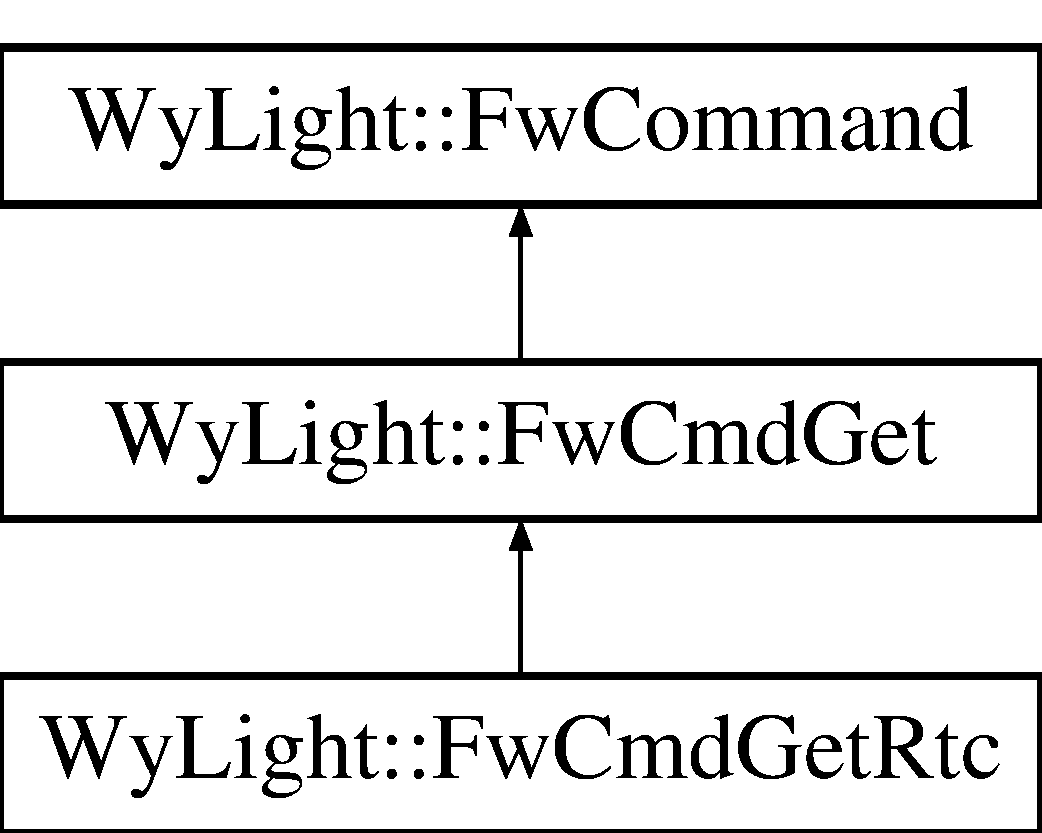
\includegraphics[height=3.000000cm]{struct_wy_light_1_1_fw_cmd_get_rtc}
\end{center}
\end{figure}
\subsection*{Public Member Functions}
\begin{DoxyCompactItemize}
\item 
\hyperlink{struct_wy_light_1_1_fw_cmd_get_rtc_af98fa45b0f597139a9f21113e1a4abcf}{Fw\-Cmd\-Get\-Rtc} (void)
\item 
\hyperlink{class_wy_light_1_1_fw_response}{Fw\-Response} \& \hyperlink{struct_wy_light_1_1_fw_cmd_get_rtc_a75ca8ea9db3216ef36367546f7726951}{Get\-Response} (void)
\end{DoxyCompactItemize}
\subsection*{Public Attributes}
\begin{DoxyCompactItemize}
\item 
\hyperlink{class_wy_light_1_1_rtc_response}{Rtc\-Response} \hyperlink{struct_wy_light_1_1_fw_cmd_get_rtc_a50e0bf16f83ee888c2bd3e1fa5d6b8ff}{m\-Response}
\end{DoxyCompactItemize}
\subsection*{Additional Inherited Members}


\subsection{Constructor \& Destructor Documentation}
\hypertarget{struct_wy_light_1_1_fw_cmd_get_rtc_af98fa45b0f597139a9f21113e1a4abcf}{\index{Wy\-Light\-::\-Fw\-Cmd\-Get\-Rtc@{Wy\-Light\-::\-Fw\-Cmd\-Get\-Rtc}!Fw\-Cmd\-Get\-Rtc@{Fw\-Cmd\-Get\-Rtc}}
\index{Fw\-Cmd\-Get\-Rtc@{Fw\-Cmd\-Get\-Rtc}!WyLight::FwCmdGetRtc@{Wy\-Light\-::\-Fw\-Cmd\-Get\-Rtc}}
\subsubsection[{Fw\-Cmd\-Get\-Rtc}]{\setlength{\rightskip}{0pt plus 5cm}Wy\-Light\-::\-Fw\-Cmd\-Get\-Rtc\-::\-Fw\-Cmd\-Get\-Rtc (
\begin{DoxyParamCaption}
\item[{void}]{}
\end{DoxyParamCaption}
)\hspace{0.3cm}{\ttfamily [inline]}}}\label{struct_wy_light_1_1_fw_cmd_get_rtc_af98fa45b0f597139a9f21113e1a4abcf}


\subsection{Member Function Documentation}
\hypertarget{struct_wy_light_1_1_fw_cmd_get_rtc_a75ca8ea9db3216ef36367546f7726951}{\index{Wy\-Light\-::\-Fw\-Cmd\-Get\-Rtc@{Wy\-Light\-::\-Fw\-Cmd\-Get\-Rtc}!Get\-Response@{Get\-Response}}
\index{Get\-Response@{Get\-Response}!WyLight::FwCmdGetRtc@{Wy\-Light\-::\-Fw\-Cmd\-Get\-Rtc}}
\subsubsection[{Get\-Response}]{\setlength{\rightskip}{0pt plus 5cm}{\bf Fw\-Response}\& Wy\-Light\-::\-Fw\-Cmd\-Get\-Rtc\-::\-Get\-Response (
\begin{DoxyParamCaption}
\item[{void}]{}
\end{DoxyParamCaption}
)\hspace{0.3cm}{\ttfamily [inline]}, {\ttfamily [virtual]}}}\label{struct_wy_light_1_1_fw_cmd_get_rtc_a75ca8ea9db3216ef36367546f7726951}


Implements \hyperlink{class_wy_light_1_1_fw_command_a37ae4cf77fd2787a9802dbb55ef489fe}{Wy\-Light\-::\-Fw\-Command}.



\subsection{Member Data Documentation}
\hypertarget{struct_wy_light_1_1_fw_cmd_get_rtc_a50e0bf16f83ee888c2bd3e1fa5d6b8ff}{\index{Wy\-Light\-::\-Fw\-Cmd\-Get\-Rtc@{Wy\-Light\-::\-Fw\-Cmd\-Get\-Rtc}!m\-Response@{m\-Response}}
\index{m\-Response@{m\-Response}!WyLight::FwCmdGetRtc@{Wy\-Light\-::\-Fw\-Cmd\-Get\-Rtc}}
\subsubsection[{m\-Response}]{\setlength{\rightskip}{0pt plus 5cm}{\bf Rtc\-Response} Wy\-Light\-::\-Fw\-Cmd\-Get\-Rtc\-::m\-Response}}\label{struct_wy_light_1_1_fw_cmd_get_rtc_a50e0bf16f83ee888c2bd3e1fa5d6b8ff}


The documentation for this struct was generated from the following file\-:\begin{DoxyCompactItemize}
\item 
library/\hyperlink{_fw_command_8h}{Fw\-Command.\-h}\end{DoxyCompactItemize}

\hypertarget{struct_wy_light_1_1_fw_cmd_get_tracebuffer}{\section{Wy\-Light\-:\-:Fw\-Cmd\-Get\-Tracebuffer Struct Reference}
\label{struct_wy_light_1_1_fw_cmd_get_tracebuffer}\index{Wy\-Light\-::\-Fw\-Cmd\-Get\-Tracebuffer@{Wy\-Light\-::\-Fw\-Cmd\-Get\-Tracebuffer}}
}


{\ttfamily \#include $<$Fw\-Command.\-h$>$}

Inheritance diagram for Wy\-Light\-:\-:Fw\-Cmd\-Get\-Tracebuffer\-:\begin{figure}[H]
\begin{center}
\leavevmode
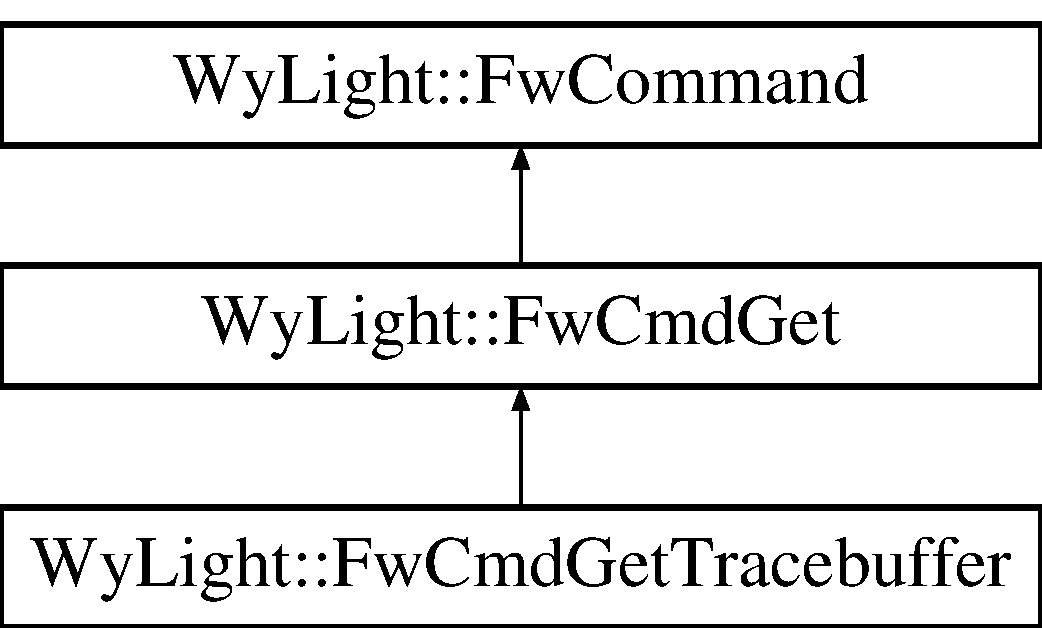
\includegraphics[height=3.000000cm]{struct_wy_light_1_1_fw_cmd_get_tracebuffer}
\end{center}
\end{figure}
\subsection*{Public Member Functions}
\begin{DoxyCompactItemize}
\item 
\hyperlink{struct_wy_light_1_1_fw_cmd_get_tracebuffer_a3deef7bcb0eafde8f9c97428da016b08}{Fw\-Cmd\-Get\-Tracebuffer} (void)
\item 
\hyperlink{class_wy_light_1_1_fw_response}{Fw\-Response} \& \hyperlink{struct_wy_light_1_1_fw_cmd_get_tracebuffer_a3c6291a4be3b4451dc1cdf1b21488d39}{Get\-Response} (void)
\end{DoxyCompactItemize}
\subsection*{Public Attributes}
\begin{DoxyCompactItemize}
\item 
\hyperlink{class_wy_light_1_1_tracebuffer_response}{Tracebuffer\-Response} \hyperlink{struct_wy_light_1_1_fw_cmd_get_tracebuffer_ae7ba6567ab462ad9237f4a35365fcb5f}{m\-Response}
\end{DoxyCompactItemize}
\subsection*{Additional Inherited Members}


\subsection{Constructor \& Destructor Documentation}
\hypertarget{struct_wy_light_1_1_fw_cmd_get_tracebuffer_a3deef7bcb0eafde8f9c97428da016b08}{\index{Wy\-Light\-::\-Fw\-Cmd\-Get\-Tracebuffer@{Wy\-Light\-::\-Fw\-Cmd\-Get\-Tracebuffer}!Fw\-Cmd\-Get\-Tracebuffer@{Fw\-Cmd\-Get\-Tracebuffer}}
\index{Fw\-Cmd\-Get\-Tracebuffer@{Fw\-Cmd\-Get\-Tracebuffer}!WyLight::FwCmdGetTracebuffer@{Wy\-Light\-::\-Fw\-Cmd\-Get\-Tracebuffer}}
\subsubsection[{Fw\-Cmd\-Get\-Tracebuffer}]{\setlength{\rightskip}{0pt plus 5cm}Wy\-Light\-::\-Fw\-Cmd\-Get\-Tracebuffer\-::\-Fw\-Cmd\-Get\-Tracebuffer (
\begin{DoxyParamCaption}
\item[{void}]{}
\end{DoxyParamCaption}
)\hspace{0.3cm}{\ttfamily [inline]}}}\label{struct_wy_light_1_1_fw_cmd_get_tracebuffer_a3deef7bcb0eafde8f9c97428da016b08}


\subsection{Member Function Documentation}
\hypertarget{struct_wy_light_1_1_fw_cmd_get_tracebuffer_a3c6291a4be3b4451dc1cdf1b21488d39}{\index{Wy\-Light\-::\-Fw\-Cmd\-Get\-Tracebuffer@{Wy\-Light\-::\-Fw\-Cmd\-Get\-Tracebuffer}!Get\-Response@{Get\-Response}}
\index{Get\-Response@{Get\-Response}!WyLight::FwCmdGetTracebuffer@{Wy\-Light\-::\-Fw\-Cmd\-Get\-Tracebuffer}}
\subsubsection[{Get\-Response}]{\setlength{\rightskip}{0pt plus 5cm}{\bf Fw\-Response}\& Wy\-Light\-::\-Fw\-Cmd\-Get\-Tracebuffer\-::\-Get\-Response (
\begin{DoxyParamCaption}
\item[{void}]{}
\end{DoxyParamCaption}
)\hspace{0.3cm}{\ttfamily [inline]}, {\ttfamily [virtual]}}}\label{struct_wy_light_1_1_fw_cmd_get_tracebuffer_a3c6291a4be3b4451dc1cdf1b21488d39}


Implements \hyperlink{class_wy_light_1_1_fw_command_a37ae4cf77fd2787a9802dbb55ef489fe}{Wy\-Light\-::\-Fw\-Command}.



\subsection{Member Data Documentation}
\hypertarget{struct_wy_light_1_1_fw_cmd_get_tracebuffer_ae7ba6567ab462ad9237f4a35365fcb5f}{\index{Wy\-Light\-::\-Fw\-Cmd\-Get\-Tracebuffer@{Wy\-Light\-::\-Fw\-Cmd\-Get\-Tracebuffer}!m\-Response@{m\-Response}}
\index{m\-Response@{m\-Response}!WyLight::FwCmdGetTracebuffer@{Wy\-Light\-::\-Fw\-Cmd\-Get\-Tracebuffer}}
\subsubsection[{m\-Response}]{\setlength{\rightskip}{0pt plus 5cm}{\bf Tracebuffer\-Response} Wy\-Light\-::\-Fw\-Cmd\-Get\-Tracebuffer\-::m\-Response}}\label{struct_wy_light_1_1_fw_cmd_get_tracebuffer_ae7ba6567ab462ad9237f4a35365fcb5f}


The documentation for this struct was generated from the following file\-:\begin{DoxyCompactItemize}
\item 
library/\hyperlink{_fw_command_8h}{Fw\-Command.\-h}\end{DoxyCompactItemize}

\hypertarget{struct_wy_light_1_1_fw_cmd_get_version}{\section{Wy\-Light\-:\-:Fw\-Cmd\-Get\-Version Struct Reference}
\label{struct_wy_light_1_1_fw_cmd_get_version}\index{Wy\-Light\-::\-Fw\-Cmd\-Get\-Version@{Wy\-Light\-::\-Fw\-Cmd\-Get\-Version}}
}


{\ttfamily \#include $<$Fw\-Command.\-h$>$}

Inheritance diagram for Wy\-Light\-:\-:Fw\-Cmd\-Get\-Version\-:\begin{figure}[H]
\begin{center}
\leavevmode
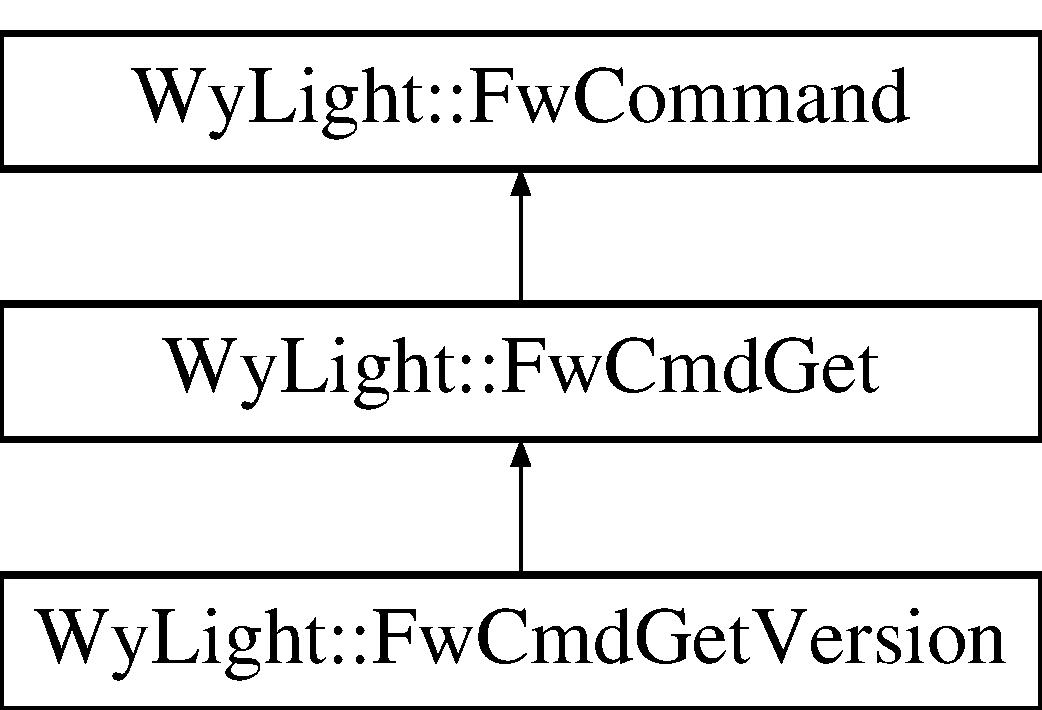
\includegraphics[height=3.000000cm]{struct_wy_light_1_1_fw_cmd_get_version}
\end{center}
\end{figure}
\subsection*{Public Member Functions}
\begin{DoxyCompactItemize}
\item 
\hyperlink{struct_wy_light_1_1_fw_cmd_get_version_a9ad3bb3337571144cf063a09d00786e2}{Fw\-Cmd\-Get\-Version} (void)
\item 
\hyperlink{class_wy_light_1_1_fw_response}{Fw\-Response} \& \hyperlink{struct_wy_light_1_1_fw_cmd_get_version_a238467662aa18499177b809d9b1d52d4}{Get\-Response} (void)
\end{DoxyCompactItemize}
\subsection*{Public Attributes}
\begin{DoxyCompactItemize}
\item 
\hyperlink{class_wy_light_1_1_firmware_version_response}{Firmware\-Version\-Response} \hyperlink{struct_wy_light_1_1_fw_cmd_get_version_aba05bc2fdb7c1aa0eb8093dc8fbe8879}{m\-Response}
\end{DoxyCompactItemize}
\subsection*{Additional Inherited Members}


\subsection{Constructor \& Destructor Documentation}
\hypertarget{struct_wy_light_1_1_fw_cmd_get_version_a9ad3bb3337571144cf063a09d00786e2}{\index{Wy\-Light\-::\-Fw\-Cmd\-Get\-Version@{Wy\-Light\-::\-Fw\-Cmd\-Get\-Version}!Fw\-Cmd\-Get\-Version@{Fw\-Cmd\-Get\-Version}}
\index{Fw\-Cmd\-Get\-Version@{Fw\-Cmd\-Get\-Version}!WyLight::FwCmdGetVersion@{Wy\-Light\-::\-Fw\-Cmd\-Get\-Version}}
\subsubsection[{Fw\-Cmd\-Get\-Version}]{\setlength{\rightskip}{0pt plus 5cm}Wy\-Light\-::\-Fw\-Cmd\-Get\-Version\-::\-Fw\-Cmd\-Get\-Version (
\begin{DoxyParamCaption}
\item[{void}]{}
\end{DoxyParamCaption}
)\hspace{0.3cm}{\ttfamily [inline]}}}\label{struct_wy_light_1_1_fw_cmd_get_version_a9ad3bb3337571144cf063a09d00786e2}


\subsection{Member Function Documentation}
\hypertarget{struct_wy_light_1_1_fw_cmd_get_version_a238467662aa18499177b809d9b1d52d4}{\index{Wy\-Light\-::\-Fw\-Cmd\-Get\-Version@{Wy\-Light\-::\-Fw\-Cmd\-Get\-Version}!Get\-Response@{Get\-Response}}
\index{Get\-Response@{Get\-Response}!WyLight::FwCmdGetVersion@{Wy\-Light\-::\-Fw\-Cmd\-Get\-Version}}
\subsubsection[{Get\-Response}]{\setlength{\rightskip}{0pt plus 5cm}{\bf Fw\-Response}\& Wy\-Light\-::\-Fw\-Cmd\-Get\-Version\-::\-Get\-Response (
\begin{DoxyParamCaption}
\item[{void}]{}
\end{DoxyParamCaption}
)\hspace{0.3cm}{\ttfamily [inline]}, {\ttfamily [virtual]}}}\label{struct_wy_light_1_1_fw_cmd_get_version_a238467662aa18499177b809d9b1d52d4}


Implements \hyperlink{class_wy_light_1_1_fw_command_a37ae4cf77fd2787a9802dbb55ef489fe}{Wy\-Light\-::\-Fw\-Command}.



\subsection{Member Data Documentation}
\hypertarget{struct_wy_light_1_1_fw_cmd_get_version_aba05bc2fdb7c1aa0eb8093dc8fbe8879}{\index{Wy\-Light\-::\-Fw\-Cmd\-Get\-Version@{Wy\-Light\-::\-Fw\-Cmd\-Get\-Version}!m\-Response@{m\-Response}}
\index{m\-Response@{m\-Response}!WyLight::FwCmdGetVersion@{Wy\-Light\-::\-Fw\-Cmd\-Get\-Version}}
\subsubsection[{m\-Response}]{\setlength{\rightskip}{0pt plus 5cm}{\bf Firmware\-Version\-Response} Wy\-Light\-::\-Fw\-Cmd\-Get\-Version\-::m\-Response}}\label{struct_wy_light_1_1_fw_cmd_get_version_aba05bc2fdb7c1aa0eb8093dc8fbe8879}


The documentation for this struct was generated from the following file\-:\begin{DoxyCompactItemize}
\item 
library/\hyperlink{_fw_command_8h}{Fw\-Command.\-h}\end{DoxyCompactItemize}

\hypertarget{struct_wy_light_1_1_fw_cmd_loop_off}{\section{Wy\-Light\-:\-:Fw\-Cmd\-Loop\-Off Struct Reference}
\label{struct_wy_light_1_1_fw_cmd_loop_off}\index{Wy\-Light\-::\-Fw\-Cmd\-Loop\-Off@{Wy\-Light\-::\-Fw\-Cmd\-Loop\-Off}}
}


{\ttfamily \#include $<$Fw\-Command.\-h$>$}

Inheritance diagram for Wy\-Light\-:\-:Fw\-Cmd\-Loop\-Off\-:\begin{figure}[H]
\begin{center}
\leavevmode
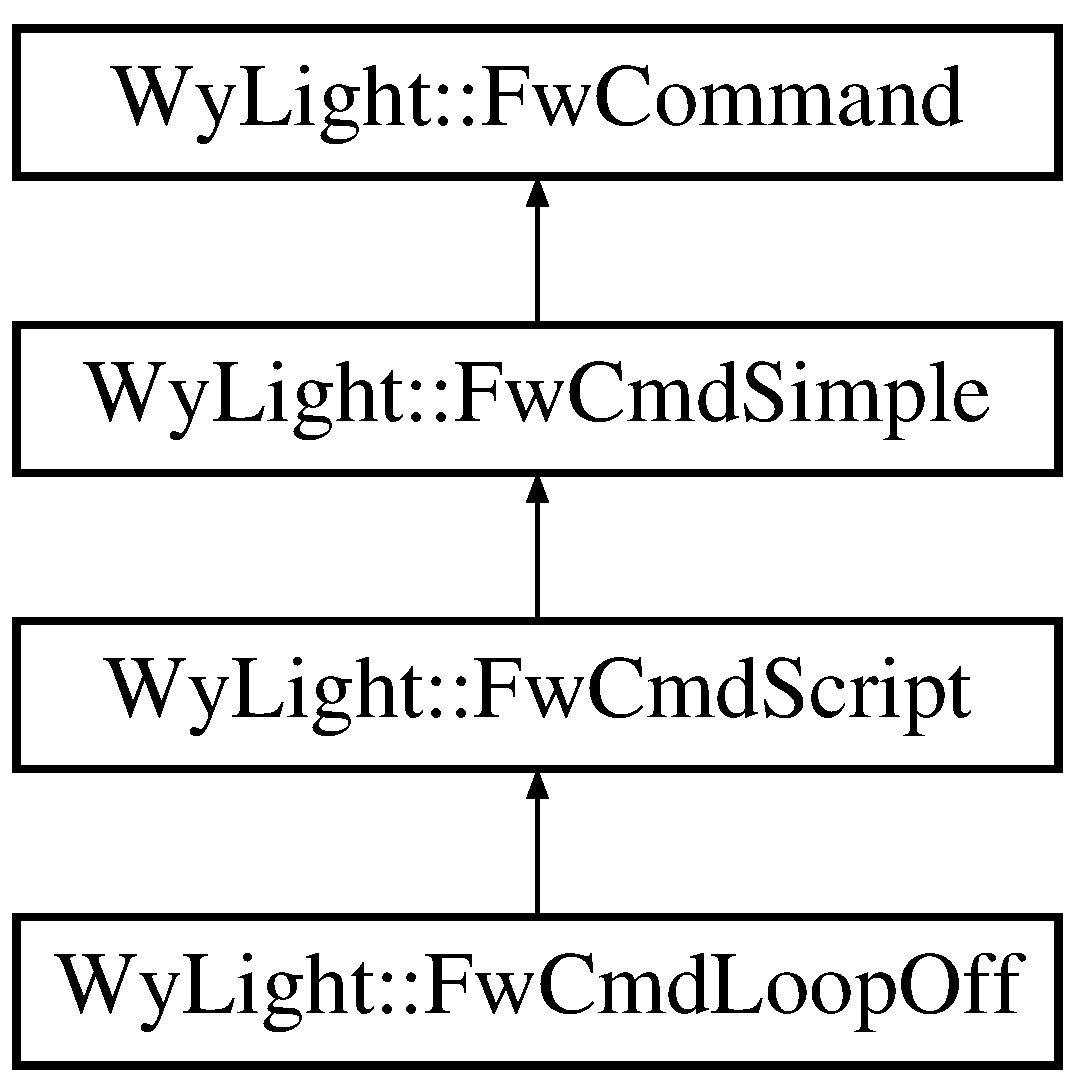
\includegraphics[height=4.000000cm]{struct_wy_light_1_1_fw_cmd_loop_off}
\end{center}
\end{figure}
\subsection*{Public Member Functions}
\begin{DoxyCompactItemize}
\item 
\hyperlink{struct_wy_light_1_1_fw_cmd_loop_off_a260dd9082278ff7b0921f775cb3b0f6d}{Fw\-Cmd\-Loop\-Off} (std\-::istream \&is)
\item 
\hyperlink{struct_wy_light_1_1_fw_cmd_loop_off_ad67156bc70cd34d22d3ade15b7bf1a20}{Fw\-Cmd\-Loop\-Off} (uint8\-\_\-t num\-Loops=0)
\item 
std\-::ostream \& \hyperlink{struct_wy_light_1_1_fw_cmd_loop_off_ac4afc42d823339073264a7e0ba1d7ad9}{Write} (std\-::ostream \&out, size\-\_\-t \&indentation) const override
\end{DoxyCompactItemize}
\subsection*{Static Public Attributes}
\begin{DoxyCompactItemize}
\item 
static const std\-::string \hyperlink{struct_wy_light_1_1_fw_cmd_loop_off_a6f9765373a55b16005a68a8735aa06b8}{T\-O\-K\-E\-N}
\end{DoxyCompactItemize}
\subsection*{Additional Inherited Members}


\subsection{Constructor \& Destructor Documentation}
\hypertarget{struct_wy_light_1_1_fw_cmd_loop_off_a260dd9082278ff7b0921f775cb3b0f6d}{\index{Wy\-Light\-::\-Fw\-Cmd\-Loop\-Off@{Wy\-Light\-::\-Fw\-Cmd\-Loop\-Off}!Fw\-Cmd\-Loop\-Off@{Fw\-Cmd\-Loop\-Off}}
\index{Fw\-Cmd\-Loop\-Off@{Fw\-Cmd\-Loop\-Off}!WyLight::FwCmdLoopOff@{Wy\-Light\-::\-Fw\-Cmd\-Loop\-Off}}
\subsubsection[{Fw\-Cmd\-Loop\-Off}]{\setlength{\rightskip}{0pt plus 5cm}Wy\-Light\-::\-Fw\-Cmd\-Loop\-Off\-::\-Fw\-Cmd\-Loop\-Off (
\begin{DoxyParamCaption}
\item[{std\-::istream \&}]{is}
\end{DoxyParamCaption}
)\hspace{0.3cm}{\ttfamily [inline]}}}\label{struct_wy_light_1_1_fw_cmd_loop_off_a260dd9082278ff7b0921f775cb3b0f6d}
\hypertarget{struct_wy_light_1_1_fw_cmd_loop_off_ad67156bc70cd34d22d3ade15b7bf1a20}{\index{Wy\-Light\-::\-Fw\-Cmd\-Loop\-Off@{Wy\-Light\-::\-Fw\-Cmd\-Loop\-Off}!Fw\-Cmd\-Loop\-Off@{Fw\-Cmd\-Loop\-Off}}
\index{Fw\-Cmd\-Loop\-Off@{Fw\-Cmd\-Loop\-Off}!WyLight::FwCmdLoopOff@{Wy\-Light\-::\-Fw\-Cmd\-Loop\-Off}}
\subsubsection[{Fw\-Cmd\-Loop\-Off}]{\setlength{\rightskip}{0pt plus 5cm}Wy\-Light\-::\-Fw\-Cmd\-Loop\-Off\-::\-Fw\-Cmd\-Loop\-Off (
\begin{DoxyParamCaption}
\item[{uint8\-\_\-t}]{num\-Loops = {\ttfamily 0}}
\end{DoxyParamCaption}
)\hspace{0.3cm}{\ttfamily [inline]}}}\label{struct_wy_light_1_1_fw_cmd_loop_off_ad67156bc70cd34d22d3ade15b7bf1a20}
Injects a Loop\-Off command into the wifly script controller 
\begin{DoxyParams}{Parameters}
{\em num\-Loops} & number of rounds before termination of the loop, use 0 for infinite loops. To terminate an infinite loop you have to send a $<$\hyperlink{struct_wy_light_1_1_fw_cmd_clear_script}{Fw\-Cmd\-Clear\-Script}$>$ \\
\hline
\end{DoxyParams}


\subsection{Member Function Documentation}
\hypertarget{struct_wy_light_1_1_fw_cmd_loop_off_ac4afc42d823339073264a7e0ba1d7ad9}{\index{Wy\-Light\-::\-Fw\-Cmd\-Loop\-Off@{Wy\-Light\-::\-Fw\-Cmd\-Loop\-Off}!Write@{Write}}
\index{Write@{Write}!WyLight::FwCmdLoopOff@{Wy\-Light\-::\-Fw\-Cmd\-Loop\-Off}}
\subsubsection[{Write}]{\setlength{\rightskip}{0pt plus 5cm}std\-::ostream\& Wy\-Light\-::\-Fw\-Cmd\-Loop\-Off\-::\-Write (
\begin{DoxyParamCaption}
\item[{std\-::ostream \&}]{out, }
\item[{size\-\_\-t \&}]{indentation}
\end{DoxyParamCaption}
) const\hspace{0.3cm}{\ttfamily [inline]}, {\ttfamily [override]}, {\ttfamily [virtual]}}}\label{struct_wy_light_1_1_fw_cmd_loop_off_ac4afc42d823339073264a7e0ba1d7ad9}


Reimplemented from \hyperlink{class_wy_light_1_1_fw_cmd_script_ad7b0c30c6787466057b109c5a5bba6b6}{Wy\-Light\-::\-Fw\-Cmd\-Script}.



\subsection{Member Data Documentation}
\hypertarget{struct_wy_light_1_1_fw_cmd_loop_off_a6f9765373a55b16005a68a8735aa06b8}{\index{Wy\-Light\-::\-Fw\-Cmd\-Loop\-Off@{Wy\-Light\-::\-Fw\-Cmd\-Loop\-Off}!T\-O\-K\-E\-N@{T\-O\-K\-E\-N}}
\index{T\-O\-K\-E\-N@{T\-O\-K\-E\-N}!WyLight::FwCmdLoopOff@{Wy\-Light\-::\-Fw\-Cmd\-Loop\-Off}}
\subsubsection[{T\-O\-K\-E\-N}]{\setlength{\rightskip}{0pt plus 5cm}const std\-::string Wy\-Light\-::\-Fw\-Cmd\-Loop\-Off\-::\-T\-O\-K\-E\-N\hspace{0.3cm}{\ttfamily [static]}}}\label{struct_wy_light_1_1_fw_cmd_loop_off_a6f9765373a55b16005a68a8735aa06b8}


The documentation for this struct was generated from the following file\-:\begin{DoxyCompactItemize}
\item 
library/\hyperlink{_fw_command_8h}{Fw\-Command.\-h}\end{DoxyCompactItemize}

\hypertarget{struct_wy_light_1_1_fw_cmd_loop_on}{\section{Wy\-Light\-:\-:Fw\-Cmd\-Loop\-On Struct Reference}
\label{struct_wy_light_1_1_fw_cmd_loop_on}\index{Wy\-Light\-::\-Fw\-Cmd\-Loop\-On@{Wy\-Light\-::\-Fw\-Cmd\-Loop\-On}}
}


{\ttfamily \#include $<$Fw\-Command.\-h$>$}

Inheritance diagram for Wy\-Light\-:\-:Fw\-Cmd\-Loop\-On\-:\begin{figure}[H]
\begin{center}
\leavevmode
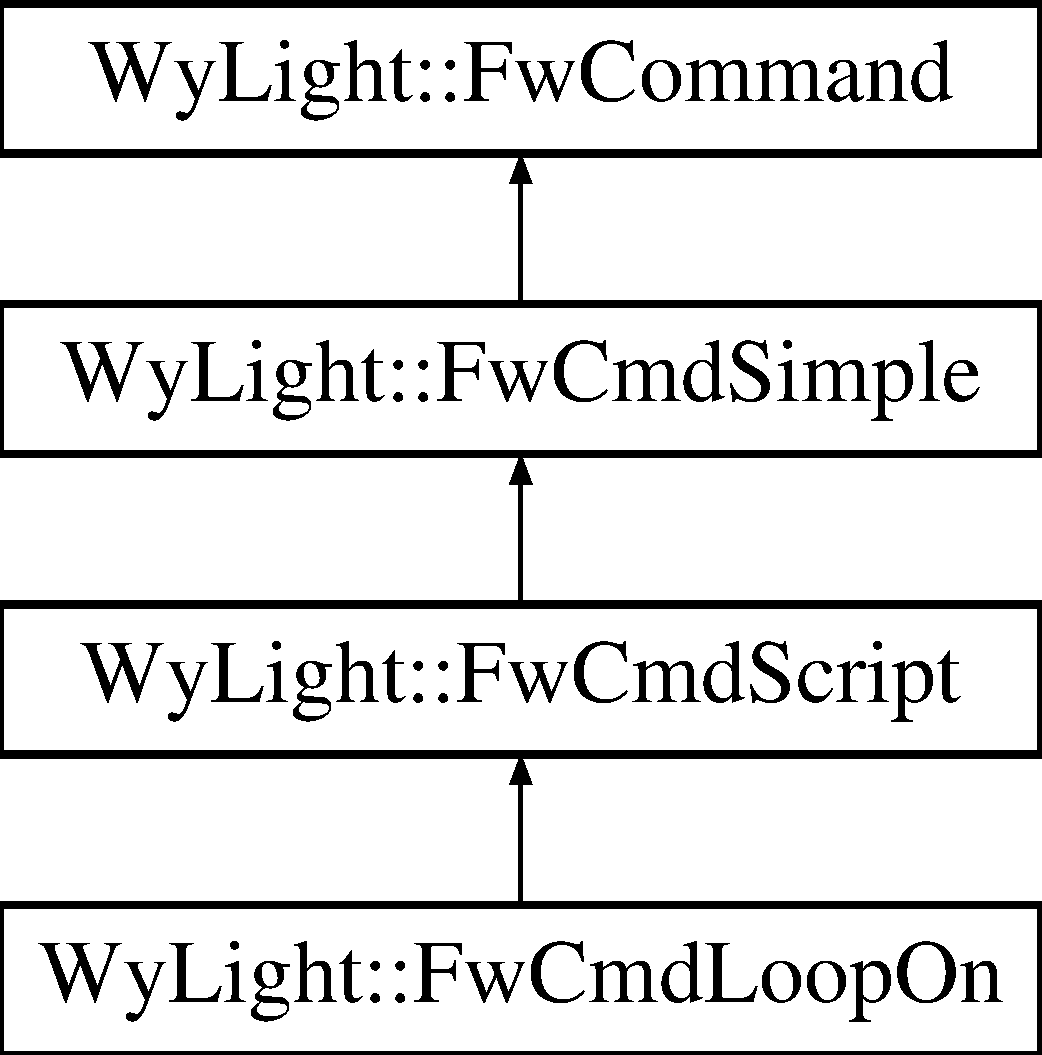
\includegraphics[height=4.000000cm]{struct_wy_light_1_1_fw_cmd_loop_on}
\end{center}
\end{figure}
\subsection*{Public Member Functions}
\begin{DoxyCompactItemize}
\item 
\hyperlink{struct_wy_light_1_1_fw_cmd_loop_on_a968bf50635e94bba35d52d2552a05cbd}{Fw\-Cmd\-Loop\-On} (void)
\item 
std\-::ostream \& \hyperlink{struct_wy_light_1_1_fw_cmd_loop_on_a07f681b0fff3b0a64017f63d1d8dfc5d}{Write} (std\-::ostream \&out, size\-\_\-t \&indentation) const override
\end{DoxyCompactItemize}
\subsection*{Static Public Attributes}
\begin{DoxyCompactItemize}
\item 
static const std\-::string \hyperlink{struct_wy_light_1_1_fw_cmd_loop_on_a58017e94f9a612a0288a010729a8e4cb}{T\-O\-K\-E\-N}
\end{DoxyCompactItemize}
\subsection*{Additional Inherited Members}


\subsection{Detailed Description}
Injects a Loop\-On command into the wifly script controller 

\subsection{Constructor \& Destructor Documentation}
\hypertarget{struct_wy_light_1_1_fw_cmd_loop_on_a968bf50635e94bba35d52d2552a05cbd}{\index{Wy\-Light\-::\-Fw\-Cmd\-Loop\-On@{Wy\-Light\-::\-Fw\-Cmd\-Loop\-On}!Fw\-Cmd\-Loop\-On@{Fw\-Cmd\-Loop\-On}}
\index{Fw\-Cmd\-Loop\-On@{Fw\-Cmd\-Loop\-On}!WyLight::FwCmdLoopOn@{Wy\-Light\-::\-Fw\-Cmd\-Loop\-On}}
\subsubsection[{Fw\-Cmd\-Loop\-On}]{\setlength{\rightskip}{0pt plus 5cm}Wy\-Light\-::\-Fw\-Cmd\-Loop\-On\-::\-Fw\-Cmd\-Loop\-On (
\begin{DoxyParamCaption}
\item[{void}]{}
\end{DoxyParamCaption}
)\hspace{0.3cm}{\ttfamily [inline]}}}\label{struct_wy_light_1_1_fw_cmd_loop_on_a968bf50635e94bba35d52d2552a05cbd}


\subsection{Member Function Documentation}
\hypertarget{struct_wy_light_1_1_fw_cmd_loop_on_a07f681b0fff3b0a64017f63d1d8dfc5d}{\index{Wy\-Light\-::\-Fw\-Cmd\-Loop\-On@{Wy\-Light\-::\-Fw\-Cmd\-Loop\-On}!Write@{Write}}
\index{Write@{Write}!WyLight::FwCmdLoopOn@{Wy\-Light\-::\-Fw\-Cmd\-Loop\-On}}
\subsubsection[{Write}]{\setlength{\rightskip}{0pt plus 5cm}std\-::ostream\& Wy\-Light\-::\-Fw\-Cmd\-Loop\-On\-::\-Write (
\begin{DoxyParamCaption}
\item[{std\-::ostream \&}]{out, }
\item[{size\-\_\-t \&}]{indentation}
\end{DoxyParamCaption}
) const\hspace{0.3cm}{\ttfamily [inline]}, {\ttfamily [override]}, {\ttfamily [virtual]}}}\label{struct_wy_light_1_1_fw_cmd_loop_on_a07f681b0fff3b0a64017f63d1d8dfc5d}


Reimplemented from \hyperlink{class_wy_light_1_1_fw_cmd_script_ad7b0c30c6787466057b109c5a5bba6b6}{Wy\-Light\-::\-Fw\-Cmd\-Script}.



\subsection{Member Data Documentation}
\hypertarget{struct_wy_light_1_1_fw_cmd_loop_on_a58017e94f9a612a0288a010729a8e4cb}{\index{Wy\-Light\-::\-Fw\-Cmd\-Loop\-On@{Wy\-Light\-::\-Fw\-Cmd\-Loop\-On}!T\-O\-K\-E\-N@{T\-O\-K\-E\-N}}
\index{T\-O\-K\-E\-N@{T\-O\-K\-E\-N}!WyLight::FwCmdLoopOn@{Wy\-Light\-::\-Fw\-Cmd\-Loop\-On}}
\subsubsection[{T\-O\-K\-E\-N}]{\setlength{\rightskip}{0pt plus 5cm}const std\-::string Wy\-Light\-::\-Fw\-Cmd\-Loop\-On\-::\-T\-O\-K\-E\-N\hspace{0.3cm}{\ttfamily [static]}}}\label{struct_wy_light_1_1_fw_cmd_loop_on_a58017e94f9a612a0288a010729a8e4cb}


The documentation for this struct was generated from the following file\-:\begin{DoxyCompactItemize}
\item 
library/\hyperlink{_fw_command_8h}{Fw\-Command.\-h}\end{DoxyCompactItemize}

\hypertarget{class_wy_light_1_1_fw_cmd_script}{\section{Wy\-Light\-:\-:Fw\-Cmd\-Script Class Reference}
\label{class_wy_light_1_1_fw_cmd_script}\index{Wy\-Light\-::\-Fw\-Cmd\-Script@{Wy\-Light\-::\-Fw\-Cmd\-Script}}
}


{\ttfamily \#include $<$Fw\-Command.\-h$>$}

Inheritance diagram for Wy\-Light\-:\-:Fw\-Cmd\-Script\-:\begin{figure}[H]
\begin{center}
\leavevmode
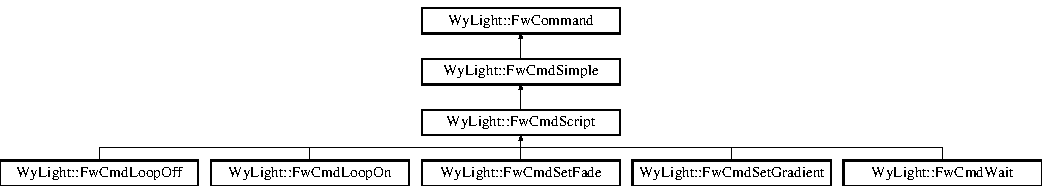
\includegraphics[height=2.502793cm]{class_wy_light_1_1_fw_cmd_script}
\end{center}
\end{figure}
\subsection*{Public Member Functions}
\begin{DoxyCompactItemize}
\item 
virtual std\-::ostream \& \hyperlink{class_wy_light_1_1_fw_cmd_script_ad7b0c30c6787466057b109c5a5bba6b6}{Write} (std\-::ostream \&out, size\-\_\-t \&indentation) const 
\end{DoxyCompactItemize}
\subsection*{Static Public Attributes}
\begin{DoxyCompactItemize}
\item 
static const size\-\_\-t \hyperlink{class_wy_light_1_1_fw_cmd_script_ab071e02170fbedc26196dece08682379}{I\-N\-D\-E\-N\-T\-A\-T\-I\-O\-N\-\_\-\-M\-A\-X} = 10
\item 
static const char \hyperlink{class_wy_light_1_1_fw_cmd_script_a8cb5ea593860ed67f2d2a0c775f9a590}{I\-N\-D\-E\-N\-T\-A\-T\-I\-O\-N\-\_\-\-C\-H\-A\-R\-A\-C\-T\-E\-R} = ' '
\end{DoxyCompactItemize}
\subsection*{Protected Member Functions}
\begin{DoxyCompactItemize}
\item 
\hyperlink{class_wy_light_1_1_fw_cmd_script_ab536f677dfe8306d3d6c13eb15198c19}{Fw\-Cmd\-Script} (uint8\-\_\-t cmd, size\-\_\-t size=0)
\end{DoxyCompactItemize}
\subsection*{Additional Inherited Members}


\subsection{Constructor \& Destructor Documentation}
\hypertarget{class_wy_light_1_1_fw_cmd_script_ab536f677dfe8306d3d6c13eb15198c19}{\index{Wy\-Light\-::\-Fw\-Cmd\-Script@{Wy\-Light\-::\-Fw\-Cmd\-Script}!Fw\-Cmd\-Script@{Fw\-Cmd\-Script}}
\index{Fw\-Cmd\-Script@{Fw\-Cmd\-Script}!WyLight::FwCmdScript@{Wy\-Light\-::\-Fw\-Cmd\-Script}}
\subsubsection[{Fw\-Cmd\-Script}]{\setlength{\rightskip}{0pt plus 5cm}Wy\-Light\-::\-Fw\-Cmd\-Script\-::\-Fw\-Cmd\-Script (
\begin{DoxyParamCaption}
\item[{uint8\-\_\-t}]{cmd, }
\item[{size\-\_\-t}]{size = {\ttfamily 0}}
\end{DoxyParamCaption}
)\hspace{0.3cm}{\ttfamily [inline]}, {\ttfamily [protected]}}}\label{class_wy_light_1_1_fw_cmd_script_ab536f677dfe8306d3d6c13eb15198c19}


\subsection{Member Function Documentation}
\hypertarget{class_wy_light_1_1_fw_cmd_script_ad7b0c30c6787466057b109c5a5bba6b6}{\index{Wy\-Light\-::\-Fw\-Cmd\-Script@{Wy\-Light\-::\-Fw\-Cmd\-Script}!Write@{Write}}
\index{Write@{Write}!WyLight::FwCmdScript@{Wy\-Light\-::\-Fw\-Cmd\-Script}}
\subsubsection[{Write}]{\setlength{\rightskip}{0pt plus 5cm}virtual std\-::ostream\& Wy\-Light\-::\-Fw\-Cmd\-Script\-::\-Write (
\begin{DoxyParamCaption}
\item[{std\-::ostream \&}]{out, }
\item[{size\-\_\-t \&}]{indentation}
\end{DoxyParamCaption}
) const\hspace{0.3cm}{\ttfamily [inline]}, {\ttfamily [virtual]}}}\label{class_wy_light_1_1_fw_cmd_script_ad7b0c30c6787466057b109c5a5bba6b6}


Reimplemented in \hyperlink{struct_wy_light_1_1_fw_cmd_set_gradient_ab29979311cc5a3e8936d634ece99f78b}{Wy\-Light\-::\-Fw\-Cmd\-Set\-Gradient}, \hyperlink{struct_wy_light_1_1_fw_cmd_set_fade_a2e6cf2016152c098c3b9706c43747010}{Wy\-Light\-::\-Fw\-Cmd\-Set\-Fade}, \hyperlink{struct_wy_light_1_1_fw_cmd_loop_on_a07f681b0fff3b0a64017f63d1d8dfc5d}{Wy\-Light\-::\-Fw\-Cmd\-Loop\-On}, \hyperlink{struct_wy_light_1_1_fw_cmd_loop_off_ac4afc42d823339073264a7e0ba1d7ad9}{Wy\-Light\-::\-Fw\-Cmd\-Loop\-Off}, and \hyperlink{class_wy_light_1_1_fw_cmd_wait_a8d96368a646e49b02058891417188d86}{Wy\-Light\-::\-Fw\-Cmd\-Wait}.



\subsection{Member Data Documentation}
\hypertarget{class_wy_light_1_1_fw_cmd_script_a8cb5ea593860ed67f2d2a0c775f9a590}{\index{Wy\-Light\-::\-Fw\-Cmd\-Script@{Wy\-Light\-::\-Fw\-Cmd\-Script}!I\-N\-D\-E\-N\-T\-A\-T\-I\-O\-N\-\_\-\-C\-H\-A\-R\-A\-C\-T\-E\-R@{I\-N\-D\-E\-N\-T\-A\-T\-I\-O\-N\-\_\-\-C\-H\-A\-R\-A\-C\-T\-E\-R}}
\index{I\-N\-D\-E\-N\-T\-A\-T\-I\-O\-N\-\_\-\-C\-H\-A\-R\-A\-C\-T\-E\-R@{I\-N\-D\-E\-N\-T\-A\-T\-I\-O\-N\-\_\-\-C\-H\-A\-R\-A\-C\-T\-E\-R}!WyLight::FwCmdScript@{Wy\-Light\-::\-Fw\-Cmd\-Script}}
\subsubsection[{I\-N\-D\-E\-N\-T\-A\-T\-I\-O\-N\-\_\-\-C\-H\-A\-R\-A\-C\-T\-E\-R}]{\setlength{\rightskip}{0pt plus 5cm}const char Wy\-Light\-::\-Fw\-Cmd\-Script\-::\-I\-N\-D\-E\-N\-T\-A\-T\-I\-O\-N\-\_\-\-C\-H\-A\-R\-A\-C\-T\-E\-R = ' '\hspace{0.3cm}{\ttfamily [static]}}}\label{class_wy_light_1_1_fw_cmd_script_a8cb5ea593860ed67f2d2a0c775f9a590}
\hypertarget{class_wy_light_1_1_fw_cmd_script_ab071e02170fbedc26196dece08682379}{\index{Wy\-Light\-::\-Fw\-Cmd\-Script@{Wy\-Light\-::\-Fw\-Cmd\-Script}!I\-N\-D\-E\-N\-T\-A\-T\-I\-O\-N\-\_\-\-M\-A\-X@{I\-N\-D\-E\-N\-T\-A\-T\-I\-O\-N\-\_\-\-M\-A\-X}}
\index{I\-N\-D\-E\-N\-T\-A\-T\-I\-O\-N\-\_\-\-M\-A\-X@{I\-N\-D\-E\-N\-T\-A\-T\-I\-O\-N\-\_\-\-M\-A\-X}!WyLight::FwCmdScript@{Wy\-Light\-::\-Fw\-Cmd\-Script}}
\subsubsection[{I\-N\-D\-E\-N\-T\-A\-T\-I\-O\-N\-\_\-\-M\-A\-X}]{\setlength{\rightskip}{0pt plus 5cm}const size\-\_\-t Wy\-Light\-::\-Fw\-Cmd\-Script\-::\-I\-N\-D\-E\-N\-T\-A\-T\-I\-O\-N\-\_\-\-M\-A\-X = 10\hspace{0.3cm}{\ttfamily [static]}}}\label{class_wy_light_1_1_fw_cmd_script_ab071e02170fbedc26196dece08682379}


The documentation for this class was generated from the following file\-:\begin{DoxyCompactItemize}
\item 
library/\hyperlink{_fw_command_8h}{Fw\-Command.\-h}\end{DoxyCompactItemize}

\hypertarget{struct_wy_light_1_1_fw_cmd_set_color_direct}{\section{Wy\-Light\-:\-:Fw\-Cmd\-Set\-Color\-Direct Struct Reference}
\label{struct_wy_light_1_1_fw_cmd_set_color_direct}\index{Wy\-Light\-::\-Fw\-Cmd\-Set\-Color\-Direct@{Wy\-Light\-::\-Fw\-Cmd\-Set\-Color\-Direct}}
}


{\ttfamily \#include $<$Fw\-Command.\-h$>$}

Inheritance diagram for Wy\-Light\-:\-:Fw\-Cmd\-Set\-Color\-Direct\-:\begin{figure}[H]
\begin{center}
\leavevmode
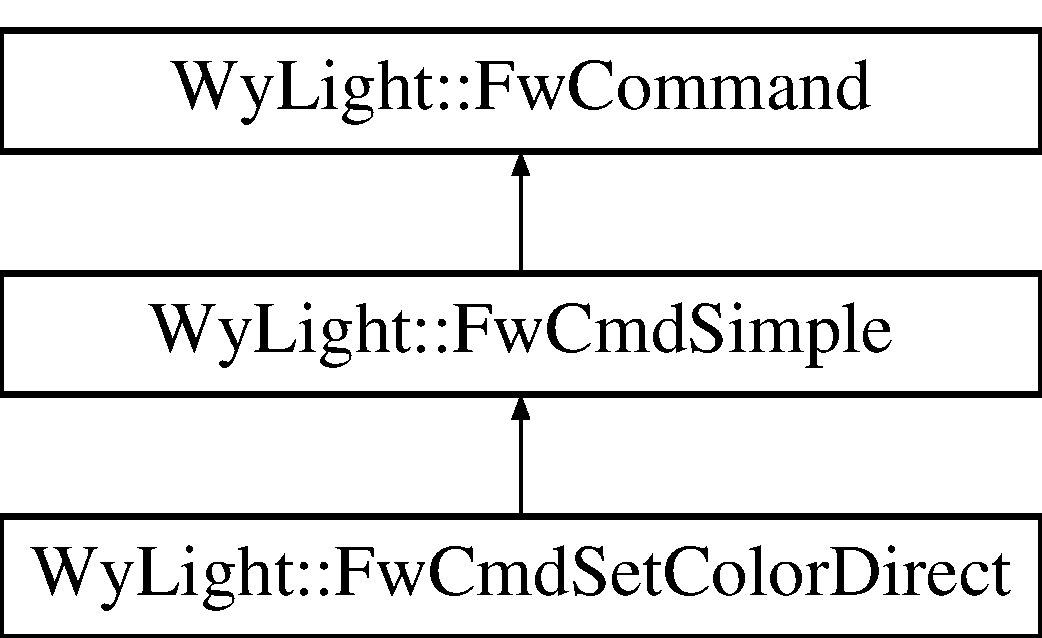
\includegraphics[height=3.000000cm]{struct_wy_light_1_1_fw_cmd_set_color_direct}
\end{center}
\end{figure}
\subsection*{Public Member Functions}
\begin{DoxyCompactItemize}
\item 
\hyperlink{struct_wy_light_1_1_fw_cmd_set_color_direct_abfae7b223f9692906dbc98e31e53c54b}{Fw\-Cmd\-Set\-Color\-Direct} (uint32\-\_\-t argb, uint32\-\_\-t addr)
\item 
\hyperlink{struct_wy_light_1_1_fw_cmd_set_color_direct_a1a82af68025d20cf7905615c4658400e}{Fw\-Cmd\-Set\-Color\-Direct} (const uint8\-\_\-t $\ast$p\-Buffer, size\-\_\-t buffer\-Length)
\end{DoxyCompactItemize}
\subsection*{Additional Inherited Members}


\subsection{Constructor \& Destructor Documentation}
\hypertarget{struct_wy_light_1_1_fw_cmd_set_color_direct_abfae7b223f9692906dbc98e31e53c54b}{\index{Wy\-Light\-::\-Fw\-Cmd\-Set\-Color\-Direct@{Wy\-Light\-::\-Fw\-Cmd\-Set\-Color\-Direct}!Fw\-Cmd\-Set\-Color\-Direct@{Fw\-Cmd\-Set\-Color\-Direct}}
\index{Fw\-Cmd\-Set\-Color\-Direct@{Fw\-Cmd\-Set\-Color\-Direct}!WyLight::FwCmdSetColorDirect@{Wy\-Light\-::\-Fw\-Cmd\-Set\-Color\-Direct}}
\subsubsection[{Fw\-Cmd\-Set\-Color\-Direct}]{\setlength{\rightskip}{0pt plus 5cm}Wy\-Light\-::\-Fw\-Cmd\-Set\-Color\-Direct\-::\-Fw\-Cmd\-Set\-Color\-Direct (
\begin{DoxyParamCaption}
\item[{uint32\-\_\-t}]{argb, }
\item[{uint32\-\_\-t}]{addr}
\end{DoxyParamCaption}
)\hspace{0.3cm}{\ttfamily [inline]}}}\label{struct_wy_light_1_1_fw_cmd_set_color_direct_abfae7b223f9692906dbc98e31e53c54b}
Sets all leds with same color directly. This doesn't affect the \hyperlink{namespace_wy_light}{Wy\-Light} script controller 
\begin{DoxyParams}{Parameters}
{\em argb} & is a 32 bit rgb value with unused alpha channel (set alpha always to 0xff) f.\-e. black(  0,  0,  0) as argb is 0xff000000 green(  0,255,  0) as argb is 0xff00ff00 white(255,255,255) as argb is 0xffffffff \\
\hline
{\em addr} & bitmask of leds which should be effected by this command, set bit to 1 to affect the led, default 0xffffffff \\
\hline
\end{DoxyParams}
\hypertarget{struct_wy_light_1_1_fw_cmd_set_color_direct_a1a82af68025d20cf7905615c4658400e}{\index{Wy\-Light\-::\-Fw\-Cmd\-Set\-Color\-Direct@{Wy\-Light\-::\-Fw\-Cmd\-Set\-Color\-Direct}!Fw\-Cmd\-Set\-Color\-Direct@{Fw\-Cmd\-Set\-Color\-Direct}}
\index{Fw\-Cmd\-Set\-Color\-Direct@{Fw\-Cmd\-Set\-Color\-Direct}!WyLight::FwCmdSetColorDirect@{Wy\-Light\-::\-Fw\-Cmd\-Set\-Color\-Direct}}
\subsubsection[{Fw\-Cmd\-Set\-Color\-Direct}]{\setlength{\rightskip}{0pt plus 5cm}Wy\-Light\-::\-Fw\-Cmd\-Set\-Color\-Direct\-::\-Fw\-Cmd\-Set\-Color\-Direct (
\begin{DoxyParamCaption}
\item[{const uint8\-\_\-t $\ast$}]{p\-Buffer, }
\item[{size\-\_\-t}]{buffer\-Length}
\end{DoxyParamCaption}
)\hspace{0.3cm}{\ttfamily [inline]}}}\label{struct_wy_light_1_1_fw_cmd_set_color_direct_a1a82af68025d20cf7905615c4658400e}
Sets all leds with different colors directly. This doesn't affect the \hyperlink{namespace_wy_light}{Wy\-Light} script controller Example\-: to set the first led to yellow and the second to blue and all others to off use a $<$p\-Buffer$>$ like this\-: p\-Buffer\mbox{[}\mbox{]} = \{0xff, 0xff, 0x00, 0x00, 0x00, 0xff\}; buffer\-Length = 6; 
\begin{DoxyParams}{Parameters}
{\em p\-Buffer} & containing continouse rgb values r1g1b1r2g2b2...r32g32b32 \\
\hline
{\em buffer\-Length} & number of bytes in $<$p\-Buffer$>$ usally 32 $\ast$ 3 bytes \\
\hline
\end{DoxyParams}


The documentation for this struct was generated from the following file\-:\begin{DoxyCompactItemize}
\item 
library/\hyperlink{_fw_command_8h}{Fw\-Command.\-h}\end{DoxyCompactItemize}

\hypertarget{struct_wy_light_1_1_fw_cmd_set_fade}{\section{Wy\-Light\-:\-:Fw\-Cmd\-Set\-Fade Struct Reference}
\label{struct_wy_light_1_1_fw_cmd_set_fade}\index{Wy\-Light\-::\-Fw\-Cmd\-Set\-Fade@{Wy\-Light\-::\-Fw\-Cmd\-Set\-Fade}}
}


{\ttfamily \#include $<$Fw\-Command.\-h$>$}

Inheritance diagram for Wy\-Light\-:\-:Fw\-Cmd\-Set\-Fade\-:\begin{figure}[H]
\begin{center}
\leavevmode
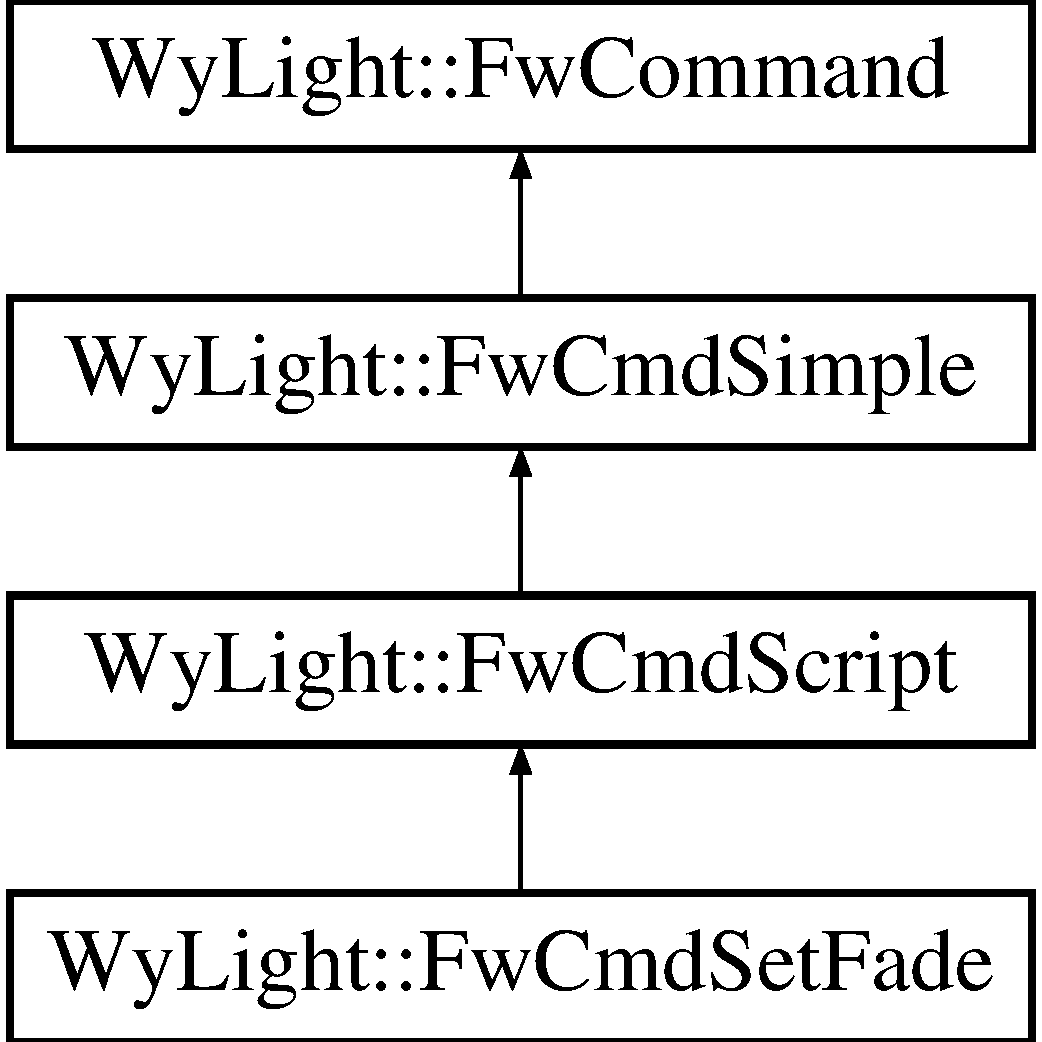
\includegraphics[height=4.000000cm]{struct_wy_light_1_1_fw_cmd_set_fade}
\end{center}
\end{figure}
\subsection*{Public Member Functions}
\begin{DoxyCompactItemize}
\item 
\hyperlink{struct_wy_light_1_1_fw_cmd_set_fade_a2338914407d05d11200e6c823d9575b0}{Fw\-Cmd\-Set\-Fade} (std\-::istream \&is)
\item 
\hyperlink{struct_wy_light_1_1_fw_cmd_set_fade_a805da076fa5c6d2aaaf31a6b9ac61f62}{Fw\-Cmd\-Set\-Fade} (uint32\-\_\-t argb, uint16\-\_\-t fade\-Time=0, uint32\-\_\-t addr=0xffffffff, bool parallel\-Fade=false)
\item 
std\-::ostream \& \hyperlink{struct_wy_light_1_1_fw_cmd_set_fade_a2e6cf2016152c098c3b9706c43747010}{Write} (std\-::ostream \&out, size\-\_\-t \&indentation) const override
\end{DoxyCompactItemize}
\subsection*{Static Public Attributes}
\begin{DoxyCompactItemize}
\item 
static const std\-::string \hyperlink{struct_wy_light_1_1_fw_cmd_set_fade_a43d478936fa849d3e3ac95775ce287b6}{T\-O\-K\-E\-N}
\end{DoxyCompactItemize}
\subsection*{Additional Inherited Members}


\subsection{Constructor \& Destructor Documentation}
\hypertarget{struct_wy_light_1_1_fw_cmd_set_fade_a2338914407d05d11200e6c823d9575b0}{\index{Wy\-Light\-::\-Fw\-Cmd\-Set\-Fade@{Wy\-Light\-::\-Fw\-Cmd\-Set\-Fade}!Fw\-Cmd\-Set\-Fade@{Fw\-Cmd\-Set\-Fade}}
\index{Fw\-Cmd\-Set\-Fade@{Fw\-Cmd\-Set\-Fade}!WyLight::FwCmdSetFade@{Wy\-Light\-::\-Fw\-Cmd\-Set\-Fade}}
\subsubsection[{Fw\-Cmd\-Set\-Fade}]{\setlength{\rightskip}{0pt plus 5cm}Wy\-Light\-::\-Fw\-Cmd\-Set\-Fade\-::\-Fw\-Cmd\-Set\-Fade (
\begin{DoxyParamCaption}
\item[{std\-::istream \&}]{is}
\end{DoxyParamCaption}
)\hspace{0.3cm}{\ttfamily [inline]}}}\label{struct_wy_light_1_1_fw_cmd_set_fade_a2338914407d05d11200e6c823d9575b0}
\hypertarget{struct_wy_light_1_1_fw_cmd_set_fade_a805da076fa5c6d2aaaf31a6b9ac61f62}{\index{Wy\-Light\-::\-Fw\-Cmd\-Set\-Fade@{Wy\-Light\-::\-Fw\-Cmd\-Set\-Fade}!Fw\-Cmd\-Set\-Fade@{Fw\-Cmd\-Set\-Fade}}
\index{Fw\-Cmd\-Set\-Fade@{Fw\-Cmd\-Set\-Fade}!WyLight::FwCmdSetFade@{Wy\-Light\-::\-Fw\-Cmd\-Set\-Fade}}
\subsubsection[{Fw\-Cmd\-Set\-Fade}]{\setlength{\rightskip}{0pt plus 5cm}Wy\-Light\-::\-Fw\-Cmd\-Set\-Fade\-::\-Fw\-Cmd\-Set\-Fade (
\begin{DoxyParamCaption}
\item[{uint32\-\_\-t}]{argb, }
\item[{uint16\-\_\-t}]{fade\-Time = {\ttfamily 0}, }
\item[{uint32\-\_\-t}]{addr = {\ttfamily 0xffffffff}, }
\item[{bool}]{parallel\-Fade = {\ttfamily false}}
\end{DoxyParamCaption}
)\hspace{0.3cm}{\ttfamily [inline]}}}\label{struct_wy_light_1_1_fw_cmd_set_fade_a805da076fa5c6d2aaaf31a6b9ac61f62}
Injects a fade command into the wifly script controller 
\begin{DoxyParams}{Parameters}
{\em argb} & is a 32 bit rgb value with unused alpha channel (set alpha always to 0xff) f.\-e. black(  0,  0,  0) as argb is 0xff000000 green(  0,255,  0) as argb is 0xff00ff00 white(255,255,255) as argb is 0xffffffff \\
\hline
{\em fade\-Time} & in hundreths of a second. Use 0 to set color immediately, default = 0 \\
\hline
{\em addr} & bitmask of leds which should be effected by this command, set bit to 1 to affect the led, default 0xffffffff \\
\hline
{\em parallel\-Fade} & if true other fades are allowed in parallel with this fade \\
\hline
\end{DoxyParams}


\subsection{Member Function Documentation}
\hypertarget{struct_wy_light_1_1_fw_cmd_set_fade_a2e6cf2016152c098c3b9706c43747010}{\index{Wy\-Light\-::\-Fw\-Cmd\-Set\-Fade@{Wy\-Light\-::\-Fw\-Cmd\-Set\-Fade}!Write@{Write}}
\index{Write@{Write}!WyLight::FwCmdSetFade@{Wy\-Light\-::\-Fw\-Cmd\-Set\-Fade}}
\subsubsection[{Write}]{\setlength{\rightskip}{0pt plus 5cm}std\-::ostream\& Wy\-Light\-::\-Fw\-Cmd\-Set\-Fade\-::\-Write (
\begin{DoxyParamCaption}
\item[{std\-::ostream \&}]{out, }
\item[{size\-\_\-t \&}]{indentation}
\end{DoxyParamCaption}
) const\hspace{0.3cm}{\ttfamily [inline]}, {\ttfamily [override]}, {\ttfamily [virtual]}}}\label{struct_wy_light_1_1_fw_cmd_set_fade_a2e6cf2016152c098c3b9706c43747010}


Reimplemented from \hyperlink{class_wy_light_1_1_fw_cmd_script_ad7b0c30c6787466057b109c5a5bba6b6}{Wy\-Light\-::\-Fw\-Cmd\-Script}.



\subsection{Member Data Documentation}
\hypertarget{struct_wy_light_1_1_fw_cmd_set_fade_a43d478936fa849d3e3ac95775ce287b6}{\index{Wy\-Light\-::\-Fw\-Cmd\-Set\-Fade@{Wy\-Light\-::\-Fw\-Cmd\-Set\-Fade}!T\-O\-K\-E\-N@{T\-O\-K\-E\-N}}
\index{T\-O\-K\-E\-N@{T\-O\-K\-E\-N}!WyLight::FwCmdSetFade@{Wy\-Light\-::\-Fw\-Cmd\-Set\-Fade}}
\subsubsection[{T\-O\-K\-E\-N}]{\setlength{\rightskip}{0pt plus 5cm}const std\-::string Wy\-Light\-::\-Fw\-Cmd\-Set\-Fade\-::\-T\-O\-K\-E\-N\hspace{0.3cm}{\ttfamily [static]}}}\label{struct_wy_light_1_1_fw_cmd_set_fade_a43d478936fa849d3e3ac95775ce287b6}


The documentation for this struct was generated from the following file\-:\begin{DoxyCompactItemize}
\item 
library/\hyperlink{_fw_command_8h}{Fw\-Command.\-h}\end{DoxyCompactItemize}

\hypertarget{struct_wy_light_1_1_fw_cmd_set_gradient}{\section{Wy\-Light\-:\-:Fw\-Cmd\-Set\-Gradient Struct Reference}
\label{struct_wy_light_1_1_fw_cmd_set_gradient}\index{Wy\-Light\-::\-Fw\-Cmd\-Set\-Gradient@{Wy\-Light\-::\-Fw\-Cmd\-Set\-Gradient}}
}


{\ttfamily \#include $<$Fw\-Command.\-h$>$}

Inheritance diagram for Wy\-Light\-:\-:Fw\-Cmd\-Set\-Gradient\-:\begin{figure}[H]
\begin{center}
\leavevmode
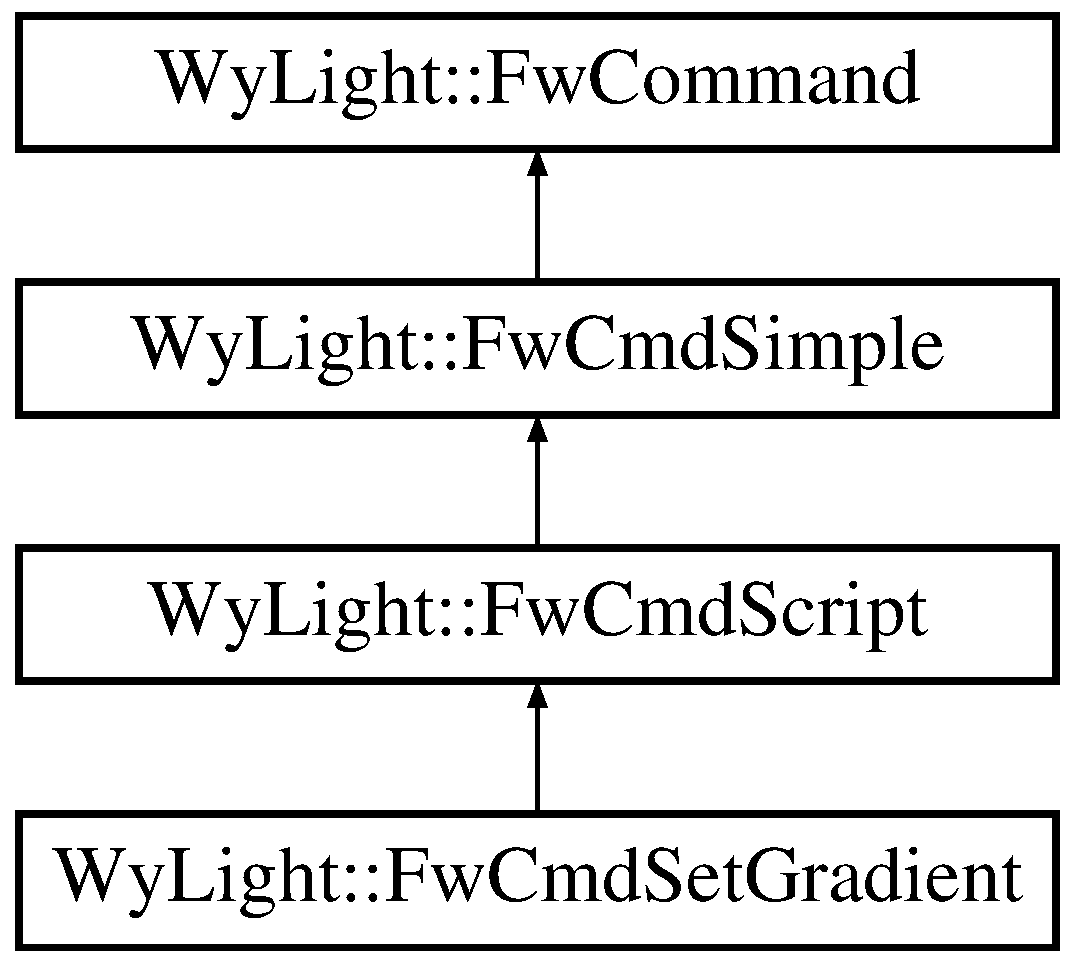
\includegraphics[height=4.000000cm]{struct_wy_light_1_1_fw_cmd_set_gradient}
\end{center}
\end{figure}
\subsection*{Public Member Functions}
\begin{DoxyCompactItemize}
\item 
\hyperlink{struct_wy_light_1_1_fw_cmd_set_gradient_a3b9481cbdee4e362825c302dfb73dd62}{Fw\-Cmd\-Set\-Gradient} (std\-::istream \&is)
\item 
\hyperlink{struct_wy_light_1_1_fw_cmd_set_gradient_a1343bc698871f4824bae187943a7fd96}{Fw\-Cmd\-Set\-Gradient} (uint32\-\_\-t argb\-\_\-1, uint32\-\_\-t argb\-\_\-2, uint16\-\_\-t fade\-Time=0, bool parallel\-Fade=false, uint8\-\_\-t length=N\-U\-M\-\_\-\-O\-F\-\_\-\-L\-E\-D, uint8\-\_\-t offset=0)
\item 
std\-::ostream \& \hyperlink{struct_wy_light_1_1_fw_cmd_set_gradient_ab29979311cc5a3e8936d634ece99f78b}{Write} (std\-::ostream \&out, size\-\_\-t \&indentation) const override
\end{DoxyCompactItemize}
\subsection*{Static Public Attributes}
\begin{DoxyCompactItemize}
\item 
static const std\-::string \hyperlink{struct_wy_light_1_1_fw_cmd_set_gradient_a2e00c35a708bdd084af9fa486bdbd83e}{T\-O\-K\-E\-N}
\end{DoxyCompactItemize}
\subsection*{Additional Inherited Members}


\subsection{Constructor \& Destructor Documentation}
\hypertarget{struct_wy_light_1_1_fw_cmd_set_gradient_a3b9481cbdee4e362825c302dfb73dd62}{\index{Wy\-Light\-::\-Fw\-Cmd\-Set\-Gradient@{Wy\-Light\-::\-Fw\-Cmd\-Set\-Gradient}!Fw\-Cmd\-Set\-Gradient@{Fw\-Cmd\-Set\-Gradient}}
\index{Fw\-Cmd\-Set\-Gradient@{Fw\-Cmd\-Set\-Gradient}!WyLight::FwCmdSetGradient@{Wy\-Light\-::\-Fw\-Cmd\-Set\-Gradient}}
\subsubsection[{Fw\-Cmd\-Set\-Gradient}]{\setlength{\rightskip}{0pt plus 5cm}Wy\-Light\-::\-Fw\-Cmd\-Set\-Gradient\-::\-Fw\-Cmd\-Set\-Gradient (
\begin{DoxyParamCaption}
\item[{std\-::istream \&}]{is}
\end{DoxyParamCaption}
)\hspace{0.3cm}{\ttfamily [inline]}}}\label{struct_wy_light_1_1_fw_cmd_set_gradient_a3b9481cbdee4e362825c302dfb73dd62}
\hypertarget{struct_wy_light_1_1_fw_cmd_set_gradient_a1343bc698871f4824bae187943a7fd96}{\index{Wy\-Light\-::\-Fw\-Cmd\-Set\-Gradient@{Wy\-Light\-::\-Fw\-Cmd\-Set\-Gradient}!Fw\-Cmd\-Set\-Gradient@{Fw\-Cmd\-Set\-Gradient}}
\index{Fw\-Cmd\-Set\-Gradient@{Fw\-Cmd\-Set\-Gradient}!WyLight::FwCmdSetGradient@{Wy\-Light\-::\-Fw\-Cmd\-Set\-Gradient}}
\subsubsection[{Fw\-Cmd\-Set\-Gradient}]{\setlength{\rightskip}{0pt plus 5cm}Wy\-Light\-::\-Fw\-Cmd\-Set\-Gradient\-::\-Fw\-Cmd\-Set\-Gradient (
\begin{DoxyParamCaption}
\item[{uint32\-\_\-t}]{argb\-\_\-1, }
\item[{uint32\-\_\-t}]{argb\-\_\-2, }
\item[{uint16\-\_\-t}]{fade\-Time = {\ttfamily 0}, }
\item[{bool}]{parallel\-Fade = {\ttfamily false}, }
\item[{uint8\-\_\-t}]{length = {\ttfamily NUM\-\_\-OF\-\_\-LED}, }
\item[{uint8\-\_\-t}]{offset = {\ttfamily 0}}
\end{DoxyParamCaption}
)\hspace{0.3cm}{\ttfamily [inline]}}}\label{struct_wy_light_1_1_fw_cmd_set_gradient_a1343bc698871f4824bae187943a7fd96}
Injects a gradient command into the wifly script controller 
\begin{DoxyParams}{Parameters}
{\em argb\-\_\-1} & is a 32 bit rgb value with unused alpha channel (set alpha always to 0xff). This is the start color for the gradient. \\
\hline
{\em argb\-\_\-2} & is a 32 bit rgb value with unused alpha channel (set alpha always to 0xff). This is the end color for the gradient. \\
\hline
{\em fade\-Time} & in hundreths of a second. Use 0 to set color immediately, default = 0 \\
\hline
{\em parallel\-Fade} & if true other fades are allowed in parallel with this fade \\
\hline
{\em length} & is the number of led's from startposition to endposition \\
\hline
{\em offset} & can be used to move the startposition of the gradient on the ledstrip \\
\hline
\end{DoxyParams}


\subsection{Member Function Documentation}
\hypertarget{struct_wy_light_1_1_fw_cmd_set_gradient_ab29979311cc5a3e8936d634ece99f78b}{\index{Wy\-Light\-::\-Fw\-Cmd\-Set\-Gradient@{Wy\-Light\-::\-Fw\-Cmd\-Set\-Gradient}!Write@{Write}}
\index{Write@{Write}!WyLight::FwCmdSetGradient@{Wy\-Light\-::\-Fw\-Cmd\-Set\-Gradient}}
\subsubsection[{Write}]{\setlength{\rightskip}{0pt plus 5cm}std\-::ostream\& Wy\-Light\-::\-Fw\-Cmd\-Set\-Gradient\-::\-Write (
\begin{DoxyParamCaption}
\item[{std\-::ostream \&}]{out, }
\item[{size\-\_\-t \&}]{indentation}
\end{DoxyParamCaption}
) const\hspace{0.3cm}{\ttfamily [inline]}, {\ttfamily [override]}, {\ttfamily [virtual]}}}\label{struct_wy_light_1_1_fw_cmd_set_gradient_ab29979311cc5a3e8936d634ece99f78b}


Reimplemented from \hyperlink{class_wy_light_1_1_fw_cmd_script_ad7b0c30c6787466057b109c5a5bba6b6}{Wy\-Light\-::\-Fw\-Cmd\-Script}.



\subsection{Member Data Documentation}
\hypertarget{struct_wy_light_1_1_fw_cmd_set_gradient_a2e00c35a708bdd084af9fa486bdbd83e}{\index{Wy\-Light\-::\-Fw\-Cmd\-Set\-Gradient@{Wy\-Light\-::\-Fw\-Cmd\-Set\-Gradient}!T\-O\-K\-E\-N@{T\-O\-K\-E\-N}}
\index{T\-O\-K\-E\-N@{T\-O\-K\-E\-N}!WyLight::FwCmdSetGradient@{Wy\-Light\-::\-Fw\-Cmd\-Set\-Gradient}}
\subsubsection[{T\-O\-K\-E\-N}]{\setlength{\rightskip}{0pt plus 5cm}const std\-::string Wy\-Light\-::\-Fw\-Cmd\-Set\-Gradient\-::\-T\-O\-K\-E\-N\hspace{0.3cm}{\ttfamily [static]}}}\label{struct_wy_light_1_1_fw_cmd_set_gradient_a2e00c35a708bdd084af9fa486bdbd83e}


The documentation for this struct was generated from the following file\-:\begin{DoxyCompactItemize}
\item 
library/\hyperlink{_fw_command_8h}{Fw\-Command.\-h}\end{DoxyCompactItemize}

\hypertarget{struct_wy_light_1_1_fw_cmd_set_rtc}{\section{Wy\-Light\-:\-:Fw\-Cmd\-Set\-Rtc Struct Reference}
\label{struct_wy_light_1_1_fw_cmd_set_rtc}\index{Wy\-Light\-::\-Fw\-Cmd\-Set\-Rtc@{Wy\-Light\-::\-Fw\-Cmd\-Set\-Rtc}}
}


{\ttfamily \#include $<$Fw\-Command.\-h$>$}

Inheritance diagram for Wy\-Light\-:\-:Fw\-Cmd\-Set\-Rtc\-:\begin{figure}[H]
\begin{center}
\leavevmode
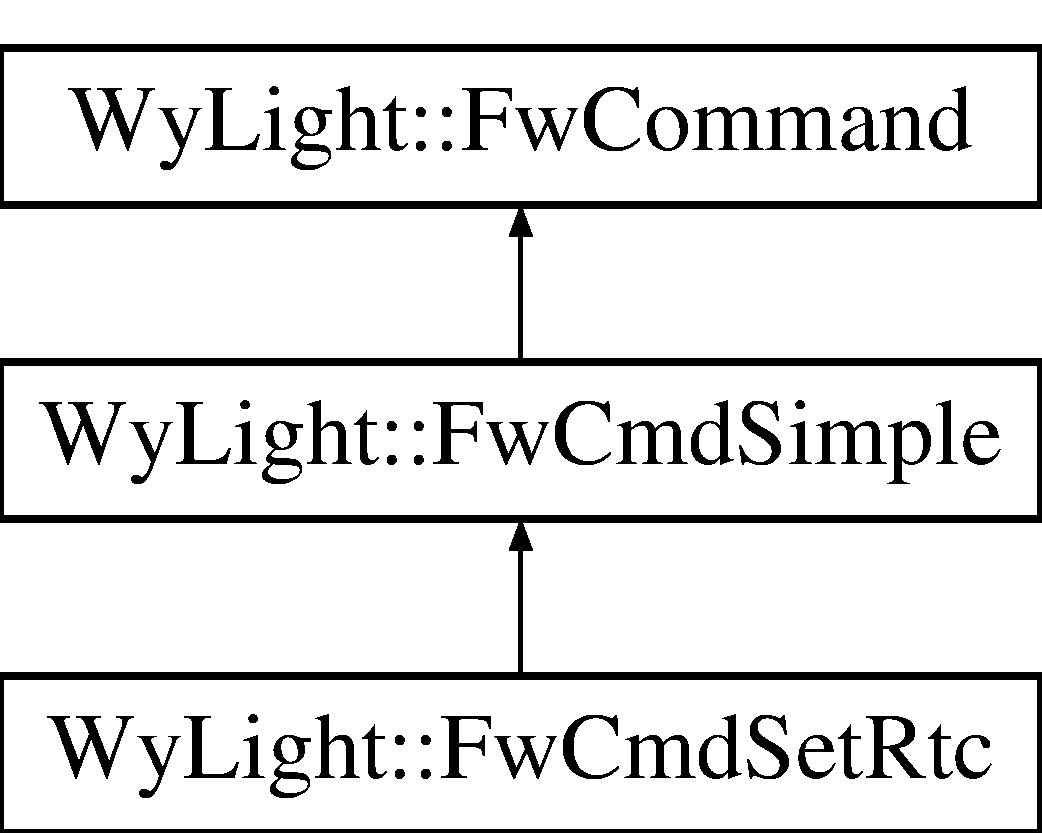
\includegraphics[height=3.000000cm]{struct_wy_light_1_1_fw_cmd_set_rtc}
\end{center}
\end{figure}
\subsection*{Public Member Functions}
\begin{DoxyCompactItemize}
\item 
\hyperlink{struct_wy_light_1_1_fw_cmd_set_rtc_afdf9d32595b1eb9d5bf27a06fd02545a}{Fw\-Cmd\-Set\-Rtc} (void)
\item 
\hyperlink{struct_wy_light_1_1_fw_cmd_set_rtc_a791e1c7e9cf3ca8c53e236599e890f41}{Fw\-Cmd\-Set\-Rtc} (const tm \&time\-Value)
\end{DoxyCompactItemize}
\subsection*{Additional Inherited Members}


\subsection{Constructor \& Destructor Documentation}
\hypertarget{struct_wy_light_1_1_fw_cmd_set_rtc_afdf9d32595b1eb9d5bf27a06fd02545a}{\index{Wy\-Light\-::\-Fw\-Cmd\-Set\-Rtc@{Wy\-Light\-::\-Fw\-Cmd\-Set\-Rtc}!Fw\-Cmd\-Set\-Rtc@{Fw\-Cmd\-Set\-Rtc}}
\index{Fw\-Cmd\-Set\-Rtc@{Fw\-Cmd\-Set\-Rtc}!WyLight::FwCmdSetRtc@{Wy\-Light\-::\-Fw\-Cmd\-Set\-Rtc}}
\subsubsection[{Fw\-Cmd\-Set\-Rtc}]{\setlength{\rightskip}{0pt plus 5cm}Wy\-Light\-::\-Fw\-Cmd\-Set\-Rtc\-::\-Fw\-Cmd\-Set\-Rtc (
\begin{DoxyParamCaption}
\item[{void}]{}
\end{DoxyParamCaption}
)\hspace{0.3cm}{\ttfamily [inline]}}}\label{struct_wy_light_1_1_fw_cmd_set_rtc_afdf9d32595b1eb9d5bf27a06fd02545a}
Sets the rtc clock of the wifly device to the current time. The wifly device has to be in firmware mode for this command. \hypertarget{struct_wy_light_1_1_fw_cmd_set_rtc_a791e1c7e9cf3ca8c53e236599e890f41}{\index{Wy\-Light\-::\-Fw\-Cmd\-Set\-Rtc@{Wy\-Light\-::\-Fw\-Cmd\-Set\-Rtc}!Fw\-Cmd\-Set\-Rtc@{Fw\-Cmd\-Set\-Rtc}}
\index{Fw\-Cmd\-Set\-Rtc@{Fw\-Cmd\-Set\-Rtc}!WyLight::FwCmdSetRtc@{Wy\-Light\-::\-Fw\-Cmd\-Set\-Rtc}}
\subsubsection[{Fw\-Cmd\-Set\-Rtc}]{\setlength{\rightskip}{0pt plus 5cm}Wy\-Light\-::\-Fw\-Cmd\-Set\-Rtc\-::\-Fw\-Cmd\-Set\-Rtc (
\begin{DoxyParamCaption}
\item[{const tm \&}]{time\-Value}
\end{DoxyParamCaption}
)\hspace{0.3cm}{\ttfamily [inline]}}}\label{struct_wy_light_1_1_fw_cmd_set_rtc_a791e1c7e9cf3ca8c53e236599e890f41}
Sets the rtc clock of the wifly device to the specified time. The wifly device has to be in firmware mode for this command. 
\begin{DoxyParams}{Parameters}
{\em time\-Value} & pointer to a posix tm struct containing the new time \\
\hline
\end{DoxyParams}


The documentation for this struct was generated from the following file\-:\begin{DoxyCompactItemize}
\item 
library/\hyperlink{_fw_command_8h}{Fw\-Command.\-h}\end{DoxyCompactItemize}

\hypertarget{class_wy_light_1_1_fw_cmd_simple}{\section{Wy\-Light\-:\-:Fw\-Cmd\-Simple Class Reference}
\label{class_wy_light_1_1_fw_cmd_simple}\index{Wy\-Light\-::\-Fw\-Cmd\-Simple@{Wy\-Light\-::\-Fw\-Cmd\-Simple}}
}


{\ttfamily \#include $<$Fw\-Command.\-h$>$}

Inheritance diagram for Wy\-Light\-:\-:Fw\-Cmd\-Simple\-:\begin{figure}[H]
\begin{center}
\leavevmode
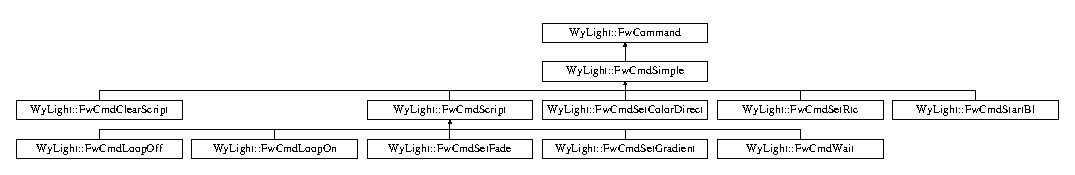
\includegraphics[height=1.904762cm]{class_wy_light_1_1_fw_cmd_simple}
\end{center}
\end{figure}
\subsection*{Public Member Functions}
\begin{DoxyCompactItemize}
\item 
\hyperlink{class_wy_light_1_1_fw_response}{Fw\-Response} \& \hyperlink{class_wy_light_1_1_fw_cmd_simple_a0d924ef07e2c70417d7300c384c9914d}{Get\-Response} (void)
\end{DoxyCompactItemize}
\subsection*{Protected Member Functions}
\begin{DoxyCompactItemize}
\item 
\hyperlink{class_wy_light_1_1_fw_cmd_simple_a402e4b55a9ba39062ea547c20dfae873}{Fw\-Cmd\-Simple} (uint8\-\_\-t cmd, size\-\_\-t size=0, bool with\-Response=true)
\end{DoxyCompactItemize}
\subsection*{Additional Inherited Members}


\subsection{Constructor \& Destructor Documentation}
\hypertarget{class_wy_light_1_1_fw_cmd_simple_a402e4b55a9ba39062ea547c20dfae873}{\index{Wy\-Light\-::\-Fw\-Cmd\-Simple@{Wy\-Light\-::\-Fw\-Cmd\-Simple}!Fw\-Cmd\-Simple@{Fw\-Cmd\-Simple}}
\index{Fw\-Cmd\-Simple@{Fw\-Cmd\-Simple}!WyLight::FwCmdSimple@{Wy\-Light\-::\-Fw\-Cmd\-Simple}}
\subsubsection[{Fw\-Cmd\-Simple}]{\setlength{\rightskip}{0pt plus 5cm}Wy\-Light\-::\-Fw\-Cmd\-Simple\-::\-Fw\-Cmd\-Simple (
\begin{DoxyParamCaption}
\item[{uint8\-\_\-t}]{cmd, }
\item[{size\-\_\-t}]{size = {\ttfamily 0}, }
\item[{bool}]{with\-Response = {\ttfamily true}}
\end{DoxyParamCaption}
)\hspace{0.3cm}{\ttfamily [inline]}, {\ttfamily [protected]}}}\label{class_wy_light_1_1_fw_cmd_simple_a402e4b55a9ba39062ea547c20dfae873}


\subsection{Member Function Documentation}
\hypertarget{class_wy_light_1_1_fw_cmd_simple_a0d924ef07e2c70417d7300c384c9914d}{\index{Wy\-Light\-::\-Fw\-Cmd\-Simple@{Wy\-Light\-::\-Fw\-Cmd\-Simple}!Get\-Response@{Get\-Response}}
\index{Get\-Response@{Get\-Response}!WyLight::FwCmdSimple@{Wy\-Light\-::\-Fw\-Cmd\-Simple}}
\subsubsection[{Get\-Response}]{\setlength{\rightskip}{0pt plus 5cm}{\bf Fw\-Response}\& Wy\-Light\-::\-Fw\-Cmd\-Simple\-::\-Get\-Response (
\begin{DoxyParamCaption}
\item[{void}]{}
\end{DoxyParamCaption}
)\hspace{0.3cm}{\ttfamily [inline]}, {\ttfamily [virtual]}}}\label{class_wy_light_1_1_fw_cmd_simple_a0d924ef07e2c70417d7300c384c9914d}


Implements \hyperlink{class_wy_light_1_1_fw_command_a37ae4cf77fd2787a9802dbb55ef489fe}{Wy\-Light\-::\-Fw\-Command}.



The documentation for this class was generated from the following file\-:\begin{DoxyCompactItemize}
\item 
library/\hyperlink{_fw_command_8h}{Fw\-Command.\-h}\end{DoxyCompactItemize}

\hypertarget{struct_wy_light_1_1_fw_cmd_start_bl}{\section{Wy\-Light\-:\-:Fw\-Cmd\-Start\-Bl Struct Reference}
\label{struct_wy_light_1_1_fw_cmd_start_bl}\index{Wy\-Light\-::\-Fw\-Cmd\-Start\-Bl@{Wy\-Light\-::\-Fw\-Cmd\-Start\-Bl}}
}


{\ttfamily \#include $<$Fw\-Command.\-h$>$}

Inheritance diagram for Wy\-Light\-:\-:Fw\-Cmd\-Start\-Bl\-:\begin{figure}[H]
\begin{center}
\leavevmode
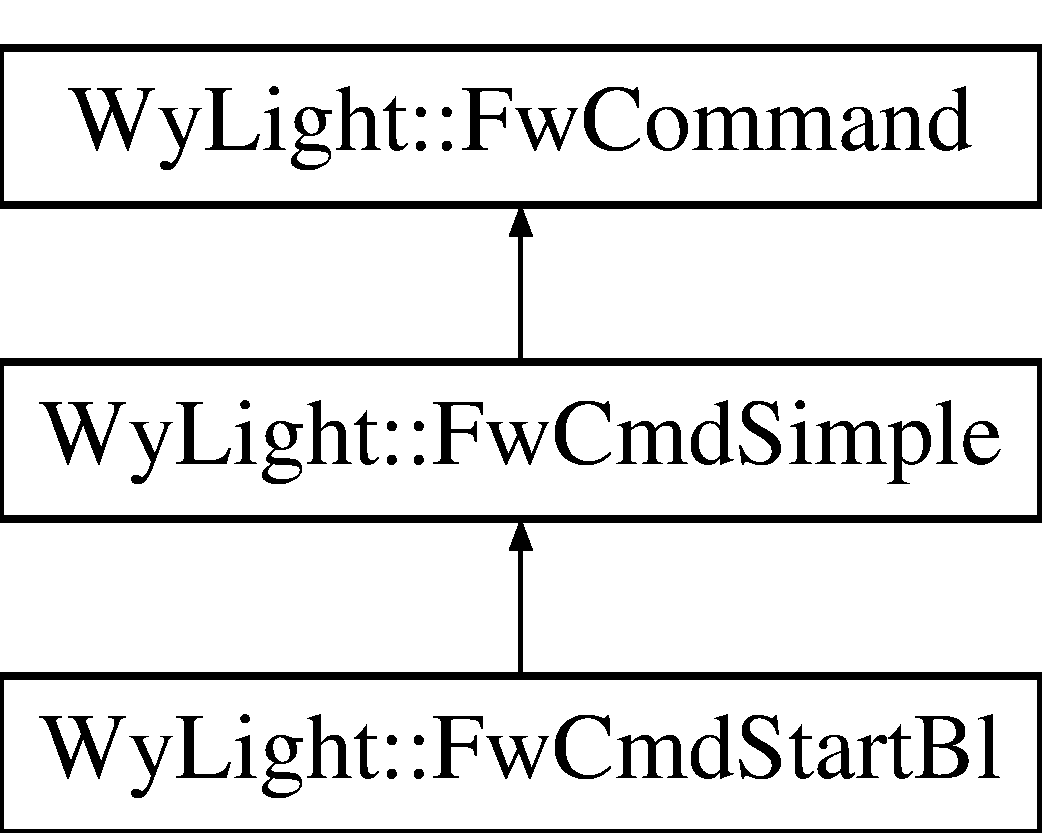
\includegraphics[height=3.000000cm]{struct_wy_light_1_1_fw_cmd_start_bl}
\end{center}
\end{figure}
\subsection*{Public Member Functions}
\begin{DoxyCompactItemize}
\item 
\hyperlink{struct_wy_light_1_1_fw_cmd_start_bl_a7a57b34e5be9ca036f9bca9df7eec1f0}{Fw\-Cmd\-Start\-Bl} (void)
\end{DoxyCompactItemize}
\subsection*{Additional Inherited Members}


\subsection{Detailed Description}
Stops firmware and script controller execution and start the bootloader of the wifly device 

\subsection{Constructor \& Destructor Documentation}
\hypertarget{struct_wy_light_1_1_fw_cmd_start_bl_a7a57b34e5be9ca036f9bca9df7eec1f0}{\index{Wy\-Light\-::\-Fw\-Cmd\-Start\-Bl@{Wy\-Light\-::\-Fw\-Cmd\-Start\-Bl}!Fw\-Cmd\-Start\-Bl@{Fw\-Cmd\-Start\-Bl}}
\index{Fw\-Cmd\-Start\-Bl@{Fw\-Cmd\-Start\-Bl}!WyLight::FwCmdStartBl@{Wy\-Light\-::\-Fw\-Cmd\-Start\-Bl}}
\subsubsection[{Fw\-Cmd\-Start\-Bl}]{\setlength{\rightskip}{0pt plus 5cm}Wy\-Light\-::\-Fw\-Cmd\-Start\-Bl\-::\-Fw\-Cmd\-Start\-Bl (
\begin{DoxyParamCaption}
\item[{void}]{}
\end{DoxyParamCaption}
)\hspace{0.3cm}{\ttfamily [inline]}}}\label{struct_wy_light_1_1_fw_cmd_start_bl_a7a57b34e5be9ca036f9bca9df7eec1f0}


The documentation for this struct was generated from the following file\-:\begin{DoxyCompactItemize}
\item 
library/\hyperlink{_fw_command_8h}{Fw\-Command.\-h}\end{DoxyCompactItemize}

\hypertarget{class_wy_light_1_1_fw_cmd_wait}{\section{Wy\-Light\-:\-:Fw\-Cmd\-Wait Class Reference}
\label{class_wy_light_1_1_fw_cmd_wait}\index{Wy\-Light\-::\-Fw\-Cmd\-Wait@{Wy\-Light\-::\-Fw\-Cmd\-Wait}}
}


{\ttfamily \#include $<$Fw\-Command.\-h$>$}

Inheritance diagram for Wy\-Light\-:\-:Fw\-Cmd\-Wait\-:\begin{figure}[H]
\begin{center}
\leavevmode
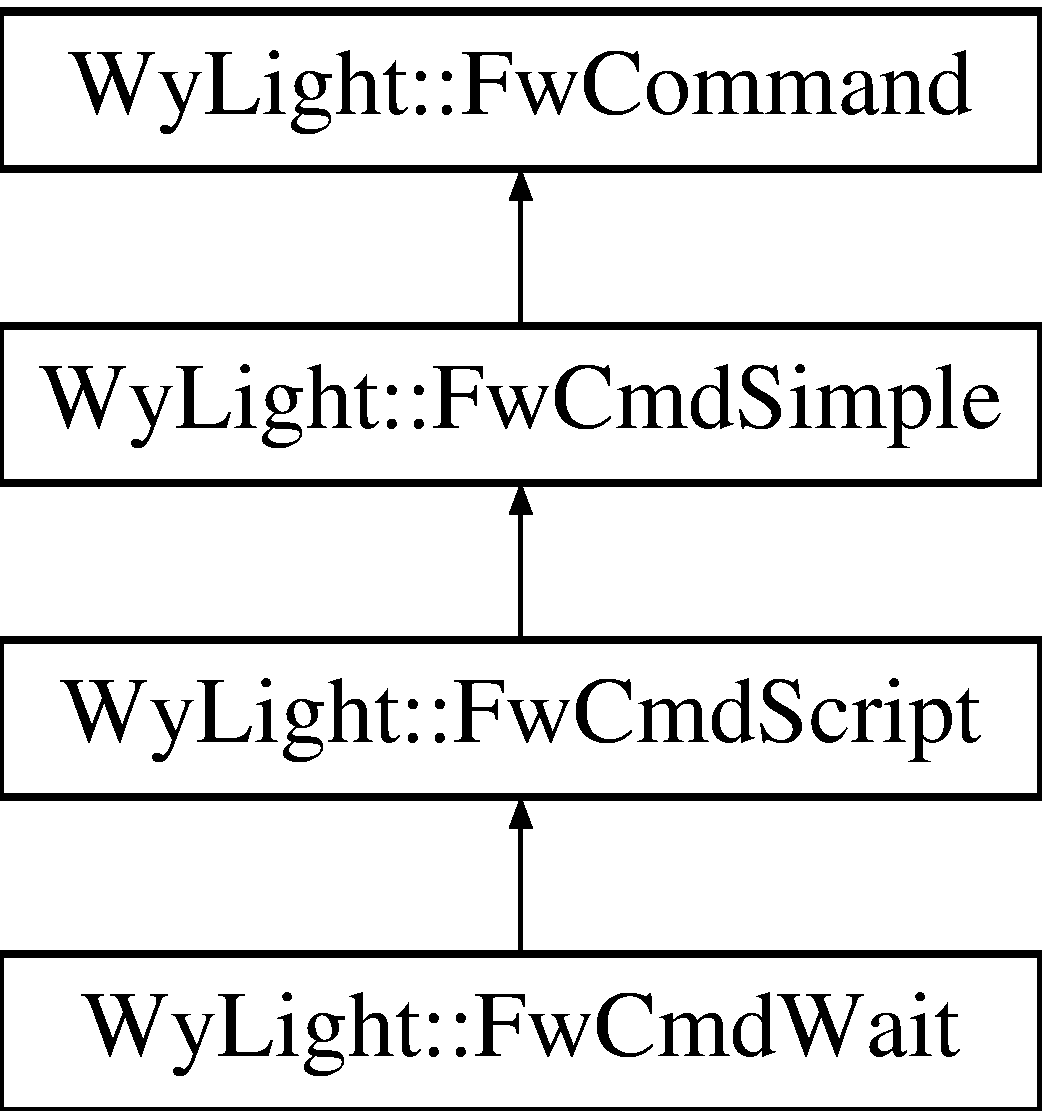
\includegraphics[height=4.000000cm]{class_wy_light_1_1_fw_cmd_wait}
\end{center}
\end{figure}
\subsection*{Public Member Functions}
\begin{DoxyCompactItemize}
\item 
\hyperlink{class_wy_light_1_1_fw_cmd_wait_aefaea11de876a87b6e77a7abb9cb5e61}{Fw\-Cmd\-Wait} (std\-::istream \&is)
\item 
\hyperlink{class_wy_light_1_1_fw_cmd_wait_acb67aeee9e9c5643c08723482f20ba35}{Fw\-Cmd\-Wait} (uint16\-\_\-t wait\-Time)
\item 
std\-::ostream \& \hyperlink{class_wy_light_1_1_fw_cmd_wait_a8d96368a646e49b02058891417188d86}{Write} (std\-::ostream \&out, size\-\_\-t \&indentation) const override
\end{DoxyCompactItemize}
\subsection*{Static Public Attributes}
\begin{DoxyCompactItemize}
\item 
static const std\-::string \hyperlink{class_wy_light_1_1_fw_cmd_wait_aee1238c424ad877171423fc3bcab31ca}{T\-O\-K\-E\-N}
\end{DoxyCompactItemize}
\subsection*{Additional Inherited Members}


\subsection{Constructor \& Destructor Documentation}
\hypertarget{class_wy_light_1_1_fw_cmd_wait_aefaea11de876a87b6e77a7abb9cb5e61}{\index{Wy\-Light\-::\-Fw\-Cmd\-Wait@{Wy\-Light\-::\-Fw\-Cmd\-Wait}!Fw\-Cmd\-Wait@{Fw\-Cmd\-Wait}}
\index{Fw\-Cmd\-Wait@{Fw\-Cmd\-Wait}!WyLight::FwCmdWait@{Wy\-Light\-::\-Fw\-Cmd\-Wait}}
\subsubsection[{Fw\-Cmd\-Wait}]{\setlength{\rightskip}{0pt plus 5cm}Wy\-Light\-::\-Fw\-Cmd\-Wait\-::\-Fw\-Cmd\-Wait (
\begin{DoxyParamCaption}
\item[{std\-::istream \&}]{is}
\end{DoxyParamCaption}
)\hspace{0.3cm}{\ttfamily [inline]}}}\label{class_wy_light_1_1_fw_cmd_wait_aefaea11de876a87b6e77a7abb9cb5e61}
\hypertarget{class_wy_light_1_1_fw_cmd_wait_acb67aeee9e9c5643c08723482f20ba35}{\index{Wy\-Light\-::\-Fw\-Cmd\-Wait@{Wy\-Light\-::\-Fw\-Cmd\-Wait}!Fw\-Cmd\-Wait@{Fw\-Cmd\-Wait}}
\index{Fw\-Cmd\-Wait@{Fw\-Cmd\-Wait}!WyLight::FwCmdWait@{Wy\-Light\-::\-Fw\-Cmd\-Wait}}
\subsubsection[{Fw\-Cmd\-Wait}]{\setlength{\rightskip}{0pt plus 5cm}Wy\-Light\-::\-Fw\-Cmd\-Wait\-::\-Fw\-Cmd\-Wait (
\begin{DoxyParamCaption}
\item[{uint16\-\_\-t}]{wait\-Time}
\end{DoxyParamCaption}
)\hspace{0.3cm}{\ttfamily [inline]}}}\label{class_wy_light_1_1_fw_cmd_wait_acb67aeee9e9c5643c08723482f20ba35}
Injects a wait command into the wifly script controller. This causes the script processing to wait before executing the next command for the specified duration 
\begin{DoxyParams}{Parameters}
{\em wait\-Time} & in hundreths of a second \\
\hline
\end{DoxyParams}


\subsection{Member Function Documentation}
\hypertarget{class_wy_light_1_1_fw_cmd_wait_a8d96368a646e49b02058891417188d86}{\index{Wy\-Light\-::\-Fw\-Cmd\-Wait@{Wy\-Light\-::\-Fw\-Cmd\-Wait}!Write@{Write}}
\index{Write@{Write}!WyLight::FwCmdWait@{Wy\-Light\-::\-Fw\-Cmd\-Wait}}
\subsubsection[{Write}]{\setlength{\rightskip}{0pt plus 5cm}std\-::ostream\& Wy\-Light\-::\-Fw\-Cmd\-Wait\-::\-Write (
\begin{DoxyParamCaption}
\item[{std\-::ostream \&}]{out, }
\item[{size\-\_\-t \&}]{indentation}
\end{DoxyParamCaption}
) const\hspace{0.3cm}{\ttfamily [inline]}, {\ttfamily [override]}, {\ttfamily [virtual]}}}\label{class_wy_light_1_1_fw_cmd_wait_a8d96368a646e49b02058891417188d86}


Reimplemented from \hyperlink{class_wy_light_1_1_fw_cmd_script_ad7b0c30c6787466057b109c5a5bba6b6}{Wy\-Light\-::\-Fw\-Cmd\-Script}.



\subsection{Member Data Documentation}
\hypertarget{class_wy_light_1_1_fw_cmd_wait_aee1238c424ad877171423fc3bcab31ca}{\index{Wy\-Light\-::\-Fw\-Cmd\-Wait@{Wy\-Light\-::\-Fw\-Cmd\-Wait}!T\-O\-K\-E\-N@{T\-O\-K\-E\-N}}
\index{T\-O\-K\-E\-N@{T\-O\-K\-E\-N}!WyLight::FwCmdWait@{Wy\-Light\-::\-Fw\-Cmd\-Wait}}
\subsubsection[{T\-O\-K\-E\-N}]{\setlength{\rightskip}{0pt plus 5cm}const std\-::string Wy\-Light\-::\-Fw\-Cmd\-Wait\-::\-T\-O\-K\-E\-N\hspace{0.3cm}{\ttfamily [static]}}}\label{class_wy_light_1_1_fw_cmd_wait_aee1238c424ad877171423fc3bcab31ca}


The documentation for this class was generated from the following file\-:\begin{DoxyCompactItemize}
\item 
library/\hyperlink{_fw_command_8h}{Fw\-Command.\-h}\end{DoxyCompactItemize}

\hypertarget{class_wy_light_1_1_fw_command}{\section{Wy\-Light\-:\-:Fw\-Command Class Reference}
\label{class_wy_light_1_1_fw_command}\index{Wy\-Light\-::\-Fw\-Command@{Wy\-Light\-::\-Fw\-Command}}
}


{\ttfamily \#include $<$Fw\-Command.\-h$>$}

Inheritance diagram for Wy\-Light\-:\-:Fw\-Command\-:\begin{figure}[H]
\begin{center}
\leavevmode
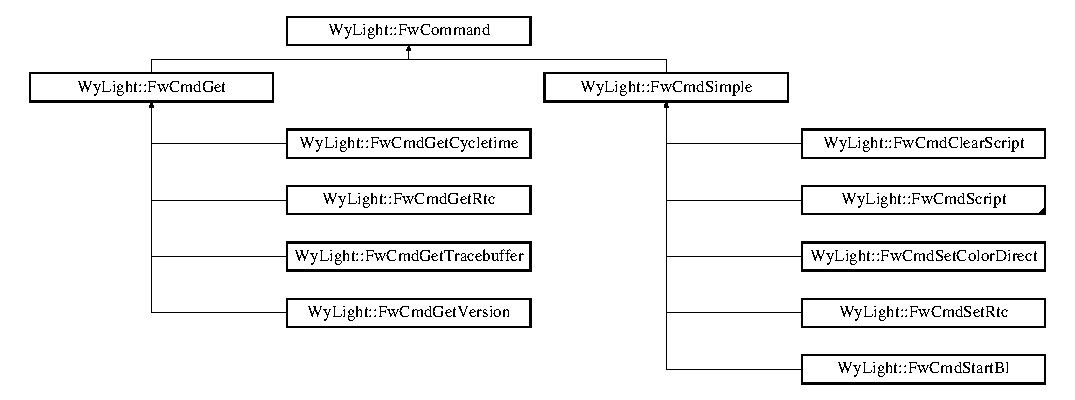
\includegraphics[height=4.924623cm]{class_wy_light_1_1_fw_command}
\end{center}
\end{figure}
\subsection*{Public Member Functions}
\begin{DoxyCompactItemize}
\item 
const uint8\-\_\-t $\ast$ \hyperlink{class_wy_light_1_1_fw_command_ad891fbb6f1a2bed364a77760c574bc68}{Get\-Data} (void) const 
\item 
size\-\_\-t \hyperlink{class_wy_light_1_1_fw_command_af45ca242c24c497039ea3063d1d2bf06}{Get\-Size} (void) const 
\item 
const bool \hyperlink{class_wy_light_1_1_fw_command_a53887169da07e23ecdeec8739acc26ce}{Is\-Response\-Required} (void) const 
\item 
virtual \hyperlink{class_wy_light_1_1_fw_response}{Fw\-Response} \& \hyperlink{class_wy_light_1_1_fw_command_a37ae4cf77fd2787a9802dbb55ef489fe}{Get\-Response} (void)=0
\item 
virtual bool \hyperlink{class_wy_light_1_1_fw_command_adad943e35162c4967a7c7f1ff44e9b66}{operator==} (const \hyperlink{class_wy_light_1_1_fw_command}{Fw\-Command} \&ref) const 
\item 
virtual bool \hyperlink{class_wy_light_1_1_fw_command_a442a3756b34059192afc65f547d67094}{operator!=} (const \hyperlink{class_wy_light_1_1_fw_command}{Fw\-Command} \&ref) const 
\end{DoxyCompactItemize}
\subsection*{Protected Member Functions}
\begin{DoxyCompactItemize}
\item 
\hyperlink{class_wy_light_1_1_fw_command_a19f7445d6240e218881903aff767b2a8}{Fw\-Command} (uint8\-\_\-t cmd, size\-\_\-t size=0, bool with\-Response=true)
\item 
virtual \hyperlink{class_wy_light_1_1_fw_command_aa3631efbb779f06a2813cdc4f44a6f48}{$\sim$\-Fw\-Command} (void)=default
\end{DoxyCompactItemize}
\subsection*{Protected Attributes}
\begin{DoxyCompactItemize}
\item 
struct led\-\_\-cmd \hyperlink{class_wy_light_1_1_fw_command_a9c16cbc6d789b240a43b95c74c608353}{m\-Req\-Frame}
\end{DoxyCompactItemize}


\subsection{Constructor \& Destructor Documentation}
\hypertarget{class_wy_light_1_1_fw_command_a19f7445d6240e218881903aff767b2a8}{\index{Wy\-Light\-::\-Fw\-Command@{Wy\-Light\-::\-Fw\-Command}!Fw\-Command@{Fw\-Command}}
\index{Fw\-Command@{Fw\-Command}!WyLight::FwCommand@{Wy\-Light\-::\-Fw\-Command}}
\subsubsection[{Fw\-Command}]{\setlength{\rightskip}{0pt plus 5cm}Wy\-Light\-::\-Fw\-Command\-::\-Fw\-Command (
\begin{DoxyParamCaption}
\item[{uint8\-\_\-t}]{cmd, }
\item[{size\-\_\-t}]{size = {\ttfamily 0}, }
\item[{bool}]{with\-Response = {\ttfamily true}}
\end{DoxyParamCaption}
)\hspace{0.3cm}{\ttfamily [inline]}, {\ttfamily [protected]}}}\label{class_wy_light_1_1_fw_command_a19f7445d6240e218881903aff767b2a8}
\hypertarget{class_wy_light_1_1_fw_command_aa3631efbb779f06a2813cdc4f44a6f48}{\index{Wy\-Light\-::\-Fw\-Command@{Wy\-Light\-::\-Fw\-Command}!$\sim$\-Fw\-Command@{$\sim$\-Fw\-Command}}
\index{$\sim$\-Fw\-Command@{$\sim$\-Fw\-Command}!WyLight::FwCommand@{Wy\-Light\-::\-Fw\-Command}}
\subsubsection[{$\sim$\-Fw\-Command}]{\setlength{\rightskip}{0pt plus 5cm}virtual Wy\-Light\-::\-Fw\-Command\-::$\sim$\-Fw\-Command (
\begin{DoxyParamCaption}
\item[{void}]{}
\end{DoxyParamCaption}
)\hspace{0.3cm}{\ttfamily [protected]}, {\ttfamily [virtual]}, {\ttfamily [default]}}}\label{class_wy_light_1_1_fw_command_aa3631efbb779f06a2813cdc4f44a6f48}


\subsection{Member Function Documentation}
\hypertarget{class_wy_light_1_1_fw_command_ad891fbb6f1a2bed364a77760c574bc68}{\index{Wy\-Light\-::\-Fw\-Command@{Wy\-Light\-::\-Fw\-Command}!Get\-Data@{Get\-Data}}
\index{Get\-Data@{Get\-Data}!WyLight::FwCommand@{Wy\-Light\-::\-Fw\-Command}}
\subsubsection[{Get\-Data}]{\setlength{\rightskip}{0pt plus 5cm}const uint8\-\_\-t$\ast$ Wy\-Light\-::\-Fw\-Command\-::\-Get\-Data (
\begin{DoxyParamCaption}
\item[{void}]{}
\end{DoxyParamCaption}
) const\hspace{0.3cm}{\ttfamily [inline]}}}\label{class_wy_light_1_1_fw_command_ad891fbb6f1a2bed364a77760c574bc68}
\hypertarget{class_wy_light_1_1_fw_command_a37ae4cf77fd2787a9802dbb55ef489fe}{\index{Wy\-Light\-::\-Fw\-Command@{Wy\-Light\-::\-Fw\-Command}!Get\-Response@{Get\-Response}}
\index{Get\-Response@{Get\-Response}!WyLight::FwCommand@{Wy\-Light\-::\-Fw\-Command}}
\subsubsection[{Get\-Response}]{\setlength{\rightskip}{0pt plus 5cm}virtual {\bf Fw\-Response}\& Wy\-Light\-::\-Fw\-Command\-::\-Get\-Response (
\begin{DoxyParamCaption}
\item[{void}]{}
\end{DoxyParamCaption}
)\hspace{0.3cm}{\ttfamily [pure virtual]}}}\label{class_wy_light_1_1_fw_command_a37ae4cf77fd2787a9802dbb55ef489fe}


Implemented in \hyperlink{struct_wy_light_1_1_fw_cmd_get_version_a238467662aa18499177b809d9b1d52d4}{Wy\-Light\-::\-Fw\-Cmd\-Get\-Version}, \hyperlink{struct_wy_light_1_1_fw_cmd_get_tracebuffer_a3c6291a4be3b4451dc1cdf1b21488d39}{Wy\-Light\-::\-Fw\-Cmd\-Get\-Tracebuffer}, \hyperlink{struct_wy_light_1_1_fw_cmd_get_rtc_a75ca8ea9db3216ef36367546f7726951}{Wy\-Light\-::\-Fw\-Cmd\-Get\-Rtc}, \hyperlink{struct_wy_light_1_1_fw_cmd_get_cycletime_aa6b457bdab92b36b2e16f88868e78beb}{Wy\-Light\-::\-Fw\-Cmd\-Get\-Cycletime}, and \hyperlink{class_wy_light_1_1_fw_cmd_simple_a0d924ef07e2c70417d7300c384c9914d}{Wy\-Light\-::\-Fw\-Cmd\-Simple}.

\hypertarget{class_wy_light_1_1_fw_command_af45ca242c24c497039ea3063d1d2bf06}{\index{Wy\-Light\-::\-Fw\-Command@{Wy\-Light\-::\-Fw\-Command}!Get\-Size@{Get\-Size}}
\index{Get\-Size@{Get\-Size}!WyLight::FwCommand@{Wy\-Light\-::\-Fw\-Command}}
\subsubsection[{Get\-Size}]{\setlength{\rightskip}{0pt plus 5cm}size\-\_\-t Wy\-Light\-::\-Fw\-Command\-::\-Get\-Size (
\begin{DoxyParamCaption}
\item[{void}]{}
\end{DoxyParamCaption}
) const\hspace{0.3cm}{\ttfamily [inline]}}}\label{class_wy_light_1_1_fw_command_af45ca242c24c497039ea3063d1d2bf06}
\hypertarget{class_wy_light_1_1_fw_command_a53887169da07e23ecdeec8739acc26ce}{\index{Wy\-Light\-::\-Fw\-Command@{Wy\-Light\-::\-Fw\-Command}!Is\-Response\-Required@{Is\-Response\-Required}}
\index{Is\-Response\-Required@{Is\-Response\-Required}!WyLight::FwCommand@{Wy\-Light\-::\-Fw\-Command}}
\subsubsection[{Is\-Response\-Required}]{\setlength{\rightskip}{0pt plus 5cm}const bool Wy\-Light\-::\-Fw\-Command\-::\-Is\-Response\-Required (
\begin{DoxyParamCaption}
\item[{void}]{}
\end{DoxyParamCaption}
) const\hspace{0.3cm}{\ttfamily [inline]}}}\label{class_wy_light_1_1_fw_command_a53887169da07e23ecdeec8739acc26ce}
\hypertarget{class_wy_light_1_1_fw_command_a442a3756b34059192afc65f547d67094}{\index{Wy\-Light\-::\-Fw\-Command@{Wy\-Light\-::\-Fw\-Command}!operator!=@{operator!=}}
\index{operator!=@{operator!=}!WyLight::FwCommand@{Wy\-Light\-::\-Fw\-Command}}
\subsubsection[{operator!=}]{\setlength{\rightskip}{0pt plus 5cm}virtual bool Wy\-Light\-::\-Fw\-Command\-::operator!= (
\begin{DoxyParamCaption}
\item[{const {\bf Fw\-Command} \&}]{ref}
\end{DoxyParamCaption}
) const\hspace{0.3cm}{\ttfamily [inline]}, {\ttfamily [virtual]}}}\label{class_wy_light_1_1_fw_command_a442a3756b34059192afc65f547d67094}
\hypertarget{class_wy_light_1_1_fw_command_adad943e35162c4967a7c7f1ff44e9b66}{\index{Wy\-Light\-::\-Fw\-Command@{Wy\-Light\-::\-Fw\-Command}!operator==@{operator==}}
\index{operator==@{operator==}!WyLight::FwCommand@{Wy\-Light\-::\-Fw\-Command}}
\subsubsection[{operator==}]{\setlength{\rightskip}{0pt plus 5cm}virtual bool Wy\-Light\-::\-Fw\-Command\-::operator== (
\begin{DoxyParamCaption}
\item[{const {\bf Fw\-Command} \&}]{ref}
\end{DoxyParamCaption}
) const\hspace{0.3cm}{\ttfamily [inline]}, {\ttfamily [virtual]}}}\label{class_wy_light_1_1_fw_command_adad943e35162c4967a7c7f1ff44e9b66}


\subsection{Member Data Documentation}
\hypertarget{class_wy_light_1_1_fw_command_a9c16cbc6d789b240a43b95c74c608353}{\index{Wy\-Light\-::\-Fw\-Command@{Wy\-Light\-::\-Fw\-Command}!m\-Req\-Frame@{m\-Req\-Frame}}
\index{m\-Req\-Frame@{m\-Req\-Frame}!WyLight::FwCommand@{Wy\-Light\-::\-Fw\-Command}}
\subsubsection[{m\-Req\-Frame}]{\setlength{\rightskip}{0pt plus 5cm}struct led\-\_\-cmd Wy\-Light\-::\-Fw\-Command\-::m\-Req\-Frame\hspace{0.3cm}{\ttfamily [protected]}}}\label{class_wy_light_1_1_fw_command_a9c16cbc6d789b240a43b95c74c608353}


The documentation for this class was generated from the following file\-:\begin{DoxyCompactItemize}
\item 
library/\hyperlink{_fw_command_8h}{Fw\-Command.\-h}\end{DoxyCompactItemize}

\hypertarget{class_wy_light_1_1_fw_response}{\section{Wy\-Light\-:\-:Fw\-Response Class Reference}
\label{class_wy_light_1_1_fw_response}\index{Wy\-Light\-::\-Fw\-Response@{Wy\-Light\-::\-Fw\-Response}}
}


{\ttfamily \#include $<$Fw\-Response.\-h$>$}

Inheritance diagram for Wy\-Light\-:\-:Fw\-Response\-:\begin{figure}[H]
\begin{center}
\leavevmode
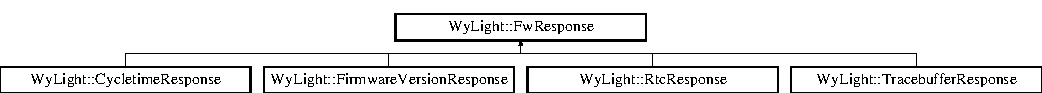
\includegraphics[height=1.255605cm]{class_wy_light_1_1_fw_response}
\end{center}
\end{figure}
\subsection*{Public Member Functions}
\begin{DoxyCompactItemize}
\item 
\hyperlink{class_wy_light_1_1_fw_response_a679566f345af722387261c8f4724e171}{Fw\-Response} (uint8\-\_\-t cmd)
\item 
virtual bool \hyperlink{class_wy_light_1_1_fw_response_aef349b4a6dd0f34c89ed8bcc8c512a55}{Init} (response\-\_\-frame \&p\-Data, const size\-\_\-t data\-Length)
\end{DoxyCompactItemize}


\subsection{Constructor \& Destructor Documentation}
\hypertarget{class_wy_light_1_1_fw_response_a679566f345af722387261c8f4724e171}{\index{Wy\-Light\-::\-Fw\-Response@{Wy\-Light\-::\-Fw\-Response}!Fw\-Response@{Fw\-Response}}
\index{Fw\-Response@{Fw\-Response}!WyLight::FwResponse@{Wy\-Light\-::\-Fw\-Response}}
\subsubsection[{Fw\-Response}]{\setlength{\rightskip}{0pt plus 5cm}Wy\-Light\-::\-Fw\-Response\-::\-Fw\-Response (
\begin{DoxyParamCaption}
\item[{uint8\-\_\-t}]{cmd}
\end{DoxyParamCaption}
)\hspace{0.3cm}{\ttfamily [inline]}}}\label{class_wy_light_1_1_fw_response_a679566f345af722387261c8f4724e171}


\subsection{Member Function Documentation}
\hypertarget{class_wy_light_1_1_fw_response_aef349b4a6dd0f34c89ed8bcc8c512a55}{\index{Wy\-Light\-::\-Fw\-Response@{Wy\-Light\-::\-Fw\-Response}!Init@{Init}}
\index{Init@{Init}!WyLight::FwResponse@{Wy\-Light\-::\-Fw\-Response}}
\subsubsection[{Init}]{\setlength{\rightskip}{0pt plus 5cm}virtual bool Wy\-Light\-::\-Fw\-Response\-::\-Init (
\begin{DoxyParamCaption}
\item[{response\-\_\-frame \&}]{p\-Data, }
\item[{const size\-\_\-t}]{data\-Length}
\end{DoxyParamCaption}
)\hspace{0.3cm}{\ttfamily [inline]}, {\ttfamily [virtual]}}}\label{class_wy_light_1_1_fw_response_aef349b4a6dd0f34c89ed8bcc8c512a55}


Reimplemented in \hyperlink{class_wy_light_1_1_firmware_version_response_ada5e917af8c5f256a11418fe5ba51211}{Wy\-Light\-::\-Firmware\-Version\-Response}, \hyperlink{class_wy_light_1_1_tracebuffer_response_a07ea006c8b97ff7b2a6e3b2de6dbd45f}{Wy\-Light\-::\-Tracebuffer\-Response}, \hyperlink{class_wy_light_1_1_cycletime_response_a44ddaaf66bed8086ad74f15d0c2d6c2a}{Wy\-Light\-::\-Cycletime\-Response}, and \hyperlink{class_wy_light_1_1_rtc_response_ab91706a872df459bba7c6dd8feab5e73}{Wy\-Light\-::\-Rtc\-Response}.



The documentation for this class was generated from the following file\-:\begin{DoxyCompactItemize}
\item 
library/\hyperlink{_fw_response_8h}{Fw\-Response.\-h}\end{DoxyCompactItemize}

\hypertarget{classintelhex}{\section{intelhex Class Reference}
\label{classintelhex}\index{intelhex@{intelhex}}
}


Class to decode, encode and manipulate Intel H\-E\-X format files.  




{\ttfamily \#include $<$intelhexclass.\-h$>$}

\subsection*{Public Member Functions}
\begin{DoxyCompactItemize}
\item 
\hyperlink{classintelhex_ae1efd0ed1f56546f8f5f5af87c6cbdd5}{intelhex} ()
\begin{DoxyCompactList}\small\item\em intelhex Class Constructor. \end{DoxyCompactList}\item 
\hyperlink{classintelhex_a031ce4582899f5263fdcc2fa92cc3e45}{$\sim$intelhex} ()
\begin{DoxyCompactList}\small\item\em intelhex Class Deconstructor. \end{DoxyCompactList}\item 
\hyperlink{classintelhex_a41b4c3b7851461b9240fdef90bc62768}{intelhex} (const \hyperlink{classintelhex}{intelhex} \&ih\-Source)
\begin{DoxyCompactList}\small\item\em intelhex Class Copy Constructor. \end{DoxyCompactList}\item 
\hyperlink{classintelhex}{intelhex} \& \hyperlink{classintelhex_a6408cc3141862454e846378abfad8ecc}{operator=} (const \hyperlink{classintelhex}{intelhex} \&ih\-Source)
\begin{DoxyCompactList}\small\item\em intelhex Class Assignment Operator. \end{DoxyCompactList}\item 
\hyperlink{classintelhex}{intelhex} \& \hyperlink{classintelhex_a044d6ab5b10a38ffa40a0b1f55b7e808}{operator++} ()
\begin{DoxyCompactList}\small\item\em Overloaded prefix increment operator. \end{DoxyCompactList}\item 
const \hyperlink{classintelhex}{intelhex} \hyperlink{classintelhex_ab54337b9681fc0b50e3fdb18ed1714fa}{operator++} (int)
\begin{DoxyCompactList}\small\item\em Overloaded postfix increment operator. \end{DoxyCompactList}\item 
\hyperlink{classintelhex}{intelhex} \& \hyperlink{classintelhex_ab85cbeafe9cc6adcec79f1bc709addca}{operator-\/-\/} ()
\begin{DoxyCompactList}\small\item\em Overloaded prefix decrement operator. \end{DoxyCompactList}\item 
const \hyperlink{classintelhex}{intelhex} \hyperlink{classintelhex_a90562846d95b5573923f129b82aeceec}{operator-\/-\/} (int)
\begin{DoxyCompactList}\small\item\em Overloaded postfix decrement operator. \end{DoxyCompactList}\item 
void \hyperlink{classintelhex_ab2b1119e14a960ea2b356967244aafb3}{begin} ()
\begin{DoxyCompactList}\small\item\em Moves the address pointer to the first available address. \end{DoxyCompactList}\item 
void \hyperlink{classintelhex_a7759926596cfcffec94e391fff4298e9}{end} ()
\begin{DoxyCompactList}\small\item\em Moves the address pointer to the last available address. \end{DoxyCompactList}\item 
unsigned long \hyperlink{classintelhex_afa757932ec420f977d33bb9a2d5a0a69}{size} ()
\begin{DoxyCompactList}\small\item\em Checks if we have reached end of available data. \end{DoxyCompactList}\item 
bool \hyperlink{classintelhex_aff915b320f5a4c2d84340fa57c99499c}{end\-Of\-Data} ()
\begin{DoxyCompactList}\small\item\em Checks if we have reached end of available data. \end{DoxyCompactList}\item 
bool \hyperlink{classintelhex_a2bd5b567207303d4d9f4322e6262d6d6}{empty} ()
\item 
bool \hyperlink{classintelhex_a83b54457c121b0f35b21b78fa2ecd712}{jump\-To} (unsigned long address)
\begin{DoxyCompactList}\small\item\em Moves the address pointer to the desired address. \end{DoxyCompactList}\item 
bool \hyperlink{classintelhex_af9c6e296e5053fe8378e79445cf480cb}{increment\-Address} ()
\begin{DoxyCompactList}\small\item\em Increments to next piece of data. \end{DoxyCompactList}\item 
bool \hyperlink{classintelhex_a51f6d93f1ac2bdf5ddad8be4e1827ce9}{decrement\-Address} ()
\begin{DoxyCompactList}\small\item\em Decrements to next piece of data. \end{DoxyCompactList}\item 
unsigned long \hyperlink{classintelhex_a631d8930daeaf04bf0d9ad9c25679a0b}{current\-Address} ()
\begin{DoxyCompactList}\small\item\em Returns the current address being pointed to. \end{DoxyCompactList}\item 
bool \hyperlink{classintelhex_aa8833665b99f0b6ac64fcef7d2116c42}{start\-Address} (unsigned long $\ast$address)
\begin{DoxyCompactList}\small\item\em Returns the lowest address currently available. \end{DoxyCompactList}\item 
bool \hyperlink{classintelhex_a9b159bea81eb832e37f6cf88a57ca659}{end\-Address} (unsigned long $\ast$address)
\begin{DoxyCompactList}\small\item\em Returns the highest address currently available. \end{DoxyCompactList}\item 
bool \hyperlink{classintelhex_a01f7799f7a86e45c28b713e9472a8a5a}{get\-Data} (unsigned char $\ast$data)
\begin{DoxyCompactList}\small\item\em Returns the data to which the iterator is currently pointing. \end{DoxyCompactList}\item 
bool \hyperlink{classintelhex_a6596b518a9a832ed8e6ba21a0e07861c}{get\-Data} (unsigned char $\ast$data, unsigned long address)
\begin{DoxyCompactList}\small\item\em Returns the data for desired address. \end{DoxyCompactList}\item 
bool \hyperlink{classintelhex_a71096983db3c24a5ac9b95663937a4ce}{insert\-Data} (unsigned char data)
\begin{DoxyCompactList}\small\item\em Inserts desired byte at the current address pointer. \end{DoxyCompactList}\item 
bool \hyperlink{classintelhex_a00ff4c491fabc5ef207071358e1b9298}{insert\-Data} (unsigned char data, unsigned long address)
\item 
void \hyperlink{classintelhex_ab4fc2715f4c63d3f31e8d2b0533583e5}{overwrite\-Data} (unsigned char data)
\item 
void \hyperlink{classintelhex_a83edcd2329cb52a4bab6bb46463184d7}{overwrite\-Data} (unsigned char data, unsigned long address)
\item 
bool \hyperlink{classintelhex_a5de5cf10103fc307127f9017f3e5cd76}{blank\-Fill} (unsigned char data)
\item 
bool \hyperlink{classintelhex_a84bbd449bb55e218b62ea73e2b399196}{blank\-Fill} (unsigned char $\ast$const data, unsigned long size\-Of\-Data)
\item 
void \hyperlink{classintelhex_aaf6f77af7a82623ef16471f105ac3fe7}{blank\-Fill} (unsigned char $\ast$const data, unsigned long size\-Of\-Data, unsigned long \hyperlink{classintelhex_a9b159bea81eb832e37f6cf88a57ca659}{end\-Address})
\item 
bool \hyperlink{classintelhex_a9c26ba3dc9dd4f3021bb6c7f6983388f}{blank\-Fill\-Random} ()
\item 
void \hyperlink{classintelhex_aa1dbcbf3df1aaafd518882c882f43f76}{blank\-Fill\-Random} (unsigned long \hyperlink{classintelhex_a9b159bea81eb832e37f6cf88a57ca659}{end\-Address})
\item 
bool \hyperlink{classintelhex_a2e5c67fccc34c78e6dbd28f4b795fb0f}{blank\-Fill\-Address\-Low\-Byte} ()
\item 
void \hyperlink{classintelhex_ab7b16f457563da93569b9812fafb9e7d}{blank\-Fill\-Address\-Low\-Byte} (unsigned long \hyperlink{classintelhex_a9b159bea81eb832e37f6cf88a57ca659}{end\-Address})
\item 
unsigned long \hyperlink{classintelhex_a05a19e1e9f1eb493a8d0bc29db88683f}{get\-No\-Warnings} ()
\begin{DoxyCompactList}\small\item\em Returns number of unread warning messages. \end{DoxyCompactList}\item 
unsigned long \hyperlink{classintelhex_a77cddd46c3f97692b4d89f138bdabb72}{get\-No\-Errors} ()
\begin{DoxyCompactList}\small\item\em Returns number of unread error messages. \end{DoxyCompactList}\item 
bool \hyperlink{classintelhex_ab881b8cb0fe665395a29e4375db8f7c4}{pop\-Next\-Warning} (string \&warning)
\begin{DoxyCompactList}\small\item\em Pop next warning message from the list of warnings. \end{DoxyCompactList}\item 
bool \hyperlink{classintelhex_a6609fd1c57a650c45a1961f6318d643e}{pop\-Next\-Error} (string \&error)
\begin{DoxyCompactList}\small\item\em Pop next error message from the list of errors. \end{DoxyCompactList}\item 
bool \hyperlink{classintelhex_a94d6d17ba22263a4775d80b2a0e6e95f}{get\-Start\-Segment\-Address} (unsigned short $\ast$\hyperlink{classintelhex_acf63100ba6ba58da893f29596560efbd}{ip\-Register}, unsigned short $\ast$\hyperlink{classintelhex_aabbf5689bc667734dca7f23a11d3df68}{cs\-Register})
\begin{DoxyCompactList}\small\item\em Returns segment start address for the I\-P and E\-S registers. \end{DoxyCompactList}\item 
bool \hyperlink{classintelhex_a7bc61f72756d37509e768906733ba10b}{get\-Start\-Linear\-Address} (unsigned long $\ast$\hyperlink{classintelhex_abedd6ca388d3cad1d2525abc5939d27e}{eip\-Register})
\begin{DoxyCompactList}\small\item\em Returns segment linear address for the E\-I\-P register. \end{DoxyCompactList}\item 
void \hyperlink{classintelhex_a9688f0002be870b05d64b5f9fcdeb86b}{set\-Start\-Segment\-Address} (unsigned short \hyperlink{classintelhex_acf63100ba6ba58da893f29596560efbd}{ip\-Register}, unsigned short \hyperlink{classintelhex_aabbf5689bc667734dca7f23a11d3df68}{cs\-Register})
\begin{DoxyCompactList}\small\item\em Sets the segment start address for the I\-P and C\-S registers. \end{DoxyCompactList}\item 
void \hyperlink{classintelhex_a7629ca097b2de02dea37fcaa2dc2709c}{set\-Start\-Linear\-Address} (unsigned long \hyperlink{classintelhex_abedd6ca388d3cad1d2525abc5939d27e}{eip\-Register})
\begin{DoxyCompactList}\small\item\em Sets the segment start address for the E\-I\-P register. \end{DoxyCompactList}\item 
void \hyperlink{classintelhex_a489fc3b9c34542def2a5167192b291da}{segment\-Addressing\-On} ()
\begin{DoxyCompactList}\small\item\em Turns on segment addressing mode during encoding. \end{DoxyCompactList}\item 
void \hyperlink{classintelhex_a5055edd337d19037ab254a27016267f8}{linear\-Addressing\-On} ()
\begin{DoxyCompactList}\small\item\em Turns on linear addressing mode during encoding. \end{DoxyCompactList}\item 
void \hyperlink{classintelhex_ac6a0119a04a2090af3ffe8c33a37cbc9}{verbose\-On} ()
\begin{DoxyCompactList}\small\item\em Turns on textual output to cout during decoding. \end{DoxyCompactList}\item 
void \hyperlink{classintelhex_a3958f077a662291bbde3472ea2bcfb4d}{verbose\-Off} ()
\begin{DoxyCompactList}\small\item\em Turns off textual output to cout during decoding. \end{DoxyCompactList}\end{DoxyCompactItemize}
\subsection*{Friends}
\begin{DoxyCompactItemize}
\item 
ostream \& \hyperlink{classintelhex_a320e23dab311a6c652aa7ddb9e2f9cc2}{operator$<$$<$} (ostream \&data\-Out, \hyperlink{classintelhex}{intelhex} \&ih\-Local)
\begin{DoxyCompactList}\small\item\em Output stream overload operator. \end{DoxyCompactList}\item 
istream \& \hyperlink{classintelhex_a73fb9c5b9d6d069b5eb83340942fd54b}{operator$>$$>$} (istream \&data\-In, \hyperlink{classintelhex}{intelhex} \&ih\-Local)
\begin{DoxyCompactList}\small\item\em Input stream overload operator. \end{DoxyCompactList}\end{DoxyCompactItemize}


\subsection{Detailed Description}
Class to decode, encode and manipulate Intel H\-E\-X format files. 

The Intel H\-E\-X class allows the user to stream in the content of an Intel H\-E\-X file so that its content can by analysed more easily than trying to decode the Intel H\-E\-X file in a text editor. In conjunction with a suitable application it is possible to create content, analyse content and even compare the content of files with one another. 

\subsection{Constructor \& Destructor Documentation}
\hypertarget{classintelhex_ae1efd0ed1f56546f8f5f5af87c6cbdd5}{\index{intelhex@{intelhex}!intelhex@{intelhex}}
\index{intelhex@{intelhex}!intelhex@{intelhex}}
\subsubsection[{intelhex}]{\setlength{\rightskip}{0pt plus 5cm}intelhex\-::intelhex (
\begin{DoxyParamCaption}
{}
\end{DoxyParamCaption}
)\hspace{0.3cm}{\ttfamily [inline]}}}\label{classintelhex_ae1efd0ed1f56546f8f5f5af87c6cbdd5}


intelhex Class Constructor. 

Important initialisation steps performed here\-:
\begin{DoxyItemize}
\item clear segment base address to zero
\item clear all x86 start address registers to zero
\item note that there are, as yet, no errors or warnings
\item note that the E\-O\-F record has not yet been found
\item set verbode mode to 'false' (default)
\item initialise class ih\-Iterator 
\end{DoxyItemize}\hypertarget{classintelhex_a031ce4582899f5263fdcc2fa92cc3e45}{\index{intelhex@{intelhex}!$\sim$intelhex@{$\sim$intelhex}}
\index{$\sim$intelhex@{$\sim$intelhex}!intelhex@{intelhex}}
\subsubsection[{$\sim$intelhex}]{\setlength{\rightskip}{0pt plus 5cm}intelhex\-::$\sim$intelhex (
\begin{DoxyParamCaption}
{}
\end{DoxyParamCaption}
)\hspace{0.3cm}{\ttfamily [inline]}}}\label{classintelhex_a031ce4582899f5263fdcc2fa92cc3e45}


intelhex Class Deconstructor. 

Currently the deconstructor is intentially empty. \hypertarget{classintelhex_a41b4c3b7851461b9240fdef90bc62768}{\index{intelhex@{intelhex}!intelhex@{intelhex}}
\index{intelhex@{intelhex}!intelhex@{intelhex}}
\subsubsection[{intelhex}]{\setlength{\rightskip}{0pt plus 5cm}intelhex\-::intelhex (
\begin{DoxyParamCaption}
\item[{const {\bf intelhex} \&}]{ih\-Source}
\end{DoxyParamCaption}
)\hspace{0.3cm}{\ttfamily [inline]}}}\label{classintelhex_a41b4c3b7851461b9240fdef90bc62768}


intelhex Class Copy Constructor. 

Copy constructor copies all essential elements for the class. 

\subsection{Member Function Documentation}
\hypertarget{classintelhex_ab2b1119e14a960ea2b356967244aafb3}{\index{intelhex@{intelhex}!begin@{begin}}
\index{begin@{begin}!intelhex@{intelhex}}
\subsubsection[{begin}]{\setlength{\rightskip}{0pt plus 5cm}void intelhex\-::begin (
\begin{DoxyParamCaption}
{}
\end{DoxyParamCaption}
)\hspace{0.3cm}{\ttfamily [inline]}}}\label{classintelhex_ab2b1119e14a960ea2b356967244aafb3}


Moves the address pointer to the first available address. 

\begin{DoxyVerb}     The address pointer will be moved to the first available address in 
     memory of the decoded file or of the data the user has inserted into
     memory for the purpose of encoding into the Intel HEX format.
\end{DoxyVerb}


\begin{DoxySeeAlso}{See Also}
\hyperlink{classintelhex_a7759926596cfcffec94e391fff4298e9}{end()}
\end{DoxySeeAlso}
\begin{DoxyNote}{Note}
This function has no effect if no file has been as yet decoded and no data has been inserted into memory. 
\end{DoxyNote}
\hypertarget{classintelhex_a5de5cf10103fc307127f9017f3e5cd76}{\index{intelhex@{intelhex}!blank\-Fill@{blank\-Fill}}
\index{blank\-Fill@{blank\-Fill}!intelhex@{intelhex}}
\subsubsection[{blank\-Fill}]{\setlength{\rightskip}{0pt plus 5cm}bool intelhex\-::blank\-Fill (
\begin{DoxyParamCaption}
\item[{unsigned char}]{data}
\end{DoxyParamCaption}
)}}\label{classintelhex_a5de5cf10103fc307127f9017f3e5cd76}
\hypertarget{classintelhex_a84bbd449bb55e218b62ea73e2b399196}{\index{intelhex@{intelhex}!blank\-Fill@{blank\-Fill}}
\index{blank\-Fill@{blank\-Fill}!intelhex@{intelhex}}
\subsubsection[{blank\-Fill}]{\setlength{\rightskip}{0pt plus 5cm}bool intelhex\-::blank\-Fill (
\begin{DoxyParamCaption}
\item[{unsigned char $\ast$const}]{data, }
\item[{unsigned long}]{size\-Of\-Data}
\end{DoxyParamCaption}
)}}\label{classintelhex_a84bbd449bb55e218b62ea73e2b399196}
\hypertarget{classintelhex_aaf6f77af7a82623ef16471f105ac3fe7}{\index{intelhex@{intelhex}!blank\-Fill@{blank\-Fill}}
\index{blank\-Fill@{blank\-Fill}!intelhex@{intelhex}}
\subsubsection[{blank\-Fill}]{\setlength{\rightskip}{0pt plus 5cm}void intelhex\-::blank\-Fill (
\begin{DoxyParamCaption}
\item[{unsigned char $\ast$const}]{data, }
\item[{unsigned long}]{size\-Of\-Data, }
\item[{unsigned long}]{end\-Address}
\end{DoxyParamCaption}
)}}\label{classintelhex_aaf6f77af7a82623ef16471f105ac3fe7}
\hypertarget{classintelhex_a2e5c67fccc34c78e6dbd28f4b795fb0f}{\index{intelhex@{intelhex}!blank\-Fill\-Address\-Low\-Byte@{blank\-Fill\-Address\-Low\-Byte}}
\index{blank\-Fill\-Address\-Low\-Byte@{blank\-Fill\-Address\-Low\-Byte}!intelhex@{intelhex}}
\subsubsection[{blank\-Fill\-Address\-Low\-Byte}]{\setlength{\rightskip}{0pt plus 5cm}bool intelhex\-::blank\-Fill\-Address\-Low\-Byte (
\begin{DoxyParamCaption}
{}
\end{DoxyParamCaption}
)}}\label{classintelhex_a2e5c67fccc34c78e6dbd28f4b795fb0f}
\hypertarget{classintelhex_ab7b16f457563da93569b9812fafb9e7d}{\index{intelhex@{intelhex}!blank\-Fill\-Address\-Low\-Byte@{blank\-Fill\-Address\-Low\-Byte}}
\index{blank\-Fill\-Address\-Low\-Byte@{blank\-Fill\-Address\-Low\-Byte}!intelhex@{intelhex}}
\subsubsection[{blank\-Fill\-Address\-Low\-Byte}]{\setlength{\rightskip}{0pt plus 5cm}void intelhex\-::blank\-Fill\-Address\-Low\-Byte (
\begin{DoxyParamCaption}
\item[{unsigned long}]{end\-Address}
\end{DoxyParamCaption}
)}}\label{classintelhex_ab7b16f457563da93569b9812fafb9e7d}
\hypertarget{classintelhex_a9c26ba3dc9dd4f3021bb6c7f6983388f}{\index{intelhex@{intelhex}!blank\-Fill\-Random@{blank\-Fill\-Random}}
\index{blank\-Fill\-Random@{blank\-Fill\-Random}!intelhex@{intelhex}}
\subsubsection[{blank\-Fill\-Random}]{\setlength{\rightskip}{0pt plus 5cm}bool intelhex\-::blank\-Fill\-Random (
\begin{DoxyParamCaption}
{}
\end{DoxyParamCaption}
)}}\label{classintelhex_a9c26ba3dc9dd4f3021bb6c7f6983388f}
\hypertarget{classintelhex_aa1dbcbf3df1aaafd518882c882f43f76}{\index{intelhex@{intelhex}!blank\-Fill\-Random@{blank\-Fill\-Random}}
\index{blank\-Fill\-Random@{blank\-Fill\-Random}!intelhex@{intelhex}}
\subsubsection[{blank\-Fill\-Random}]{\setlength{\rightskip}{0pt plus 5cm}void intelhex\-::blank\-Fill\-Random (
\begin{DoxyParamCaption}
\item[{unsigned long}]{end\-Address}
\end{DoxyParamCaption}
)}}\label{classintelhex_aa1dbcbf3df1aaafd518882c882f43f76}
\hypertarget{classintelhex_a631d8930daeaf04bf0d9ad9c25679a0b}{\index{intelhex@{intelhex}!current\-Address@{current\-Address}}
\index{current\-Address@{current\-Address}!intelhex@{intelhex}}
\subsubsection[{current\-Address}]{\setlength{\rightskip}{0pt plus 5cm}unsigned long intelhex\-::current\-Address (
\begin{DoxyParamCaption}
{}
\end{DoxyParamCaption}
)\hspace{0.3cm}{\ttfamily [inline]}}}\label{classintelhex_a631d8930daeaf04bf0d9ad9c25679a0b}


Returns the current address being pointed to. 

\begin{DoxyVerb}     Current address will be returned.
\end{DoxyVerb}


\begin{DoxySeeAlso}{See Also}
\hyperlink{classintelhex_a83b54457c121b0f35b21b78fa2ecd712}{jump\-To()}
\end{DoxySeeAlso}

\begin{DoxyRetVals}{Return values}
{\em Current} & address being pointed to. \\
\hline
\end{DoxyRetVals}
\hypertarget{classintelhex_a51f6d93f1ac2bdf5ddad8be4e1827ce9}{\index{intelhex@{intelhex}!decrement\-Address@{decrement\-Address}}
\index{decrement\-Address@{decrement\-Address}!intelhex@{intelhex}}
\subsubsection[{decrement\-Address}]{\setlength{\rightskip}{0pt plus 5cm}bool intelhex\-::decrement\-Address (
\begin{DoxyParamCaption}
{}
\end{DoxyParamCaption}
)\hspace{0.3cm}{\ttfamily [inline]}}}\label{classintelhex_a51f6d93f1ac2bdf5ddad8be4e1827ce9}


Decrements to next piece of data. 

\begin{DoxyVerb}     Address pointer will take on the address of the previous location for 
     which there is data.
\end{DoxyVerb}


\begin{DoxySeeAlso}{See Also}
\hyperlink{classintelhex_af9c6e296e5053fe8378e79445cf480cb}{increment\-Address()}
\end{DoxySeeAlso}

\begin{DoxyRetVals}{Return values}
{\em true} & -\/ pointer was decremented; a new data value was found \\
\hline
{\em false} & -\/ start of available data reached; pointer is unchanged \\
\hline
\end{DoxyRetVals}
\hypertarget{classintelhex_a2bd5b567207303d4d9f4322e6262d6d6}{\index{intelhex@{intelhex}!empty@{empty}}
\index{empty@{empty}!intelhex@{intelhex}}
\subsubsection[{empty}]{\setlength{\rightskip}{0pt plus 5cm}bool intelhex\-::empty (
\begin{DoxyParamCaption}
{}
\end{DoxyParamCaption}
)\hspace{0.3cm}{\ttfamily [inline]}}}\label{classintelhex_a2bd5b567207303d4d9f4322e6262d6d6}
\hypertarget{classintelhex_a7759926596cfcffec94e391fff4298e9}{\index{intelhex@{intelhex}!end@{end}}
\index{end@{end}!intelhex@{intelhex}}
\subsubsection[{end}]{\setlength{\rightskip}{0pt plus 5cm}void intelhex\-::end (
\begin{DoxyParamCaption}
{}
\end{DoxyParamCaption}
)\hspace{0.3cm}{\ttfamily [inline]}}}\label{classintelhex_a7759926596cfcffec94e391fff4298e9}


Moves the address pointer to the last available address. 

\begin{DoxyVerb}     The address pointer will be moved to the last available address in 
     memory of the decoded file or of the data the user has inserted into
     memory for the purpose of encoding into the Intel HEX format.
\end{DoxyVerb}


\begin{DoxySeeAlso}{See Also}
\hyperlink{classintelhex_ab2b1119e14a960ea2b356967244aafb3}{begin()}
\end{DoxySeeAlso}
\begin{DoxyNote}{Note}
This function has no effect if no file has been as yet decoded and no data has been inserted into memory. 
\end{DoxyNote}
\hypertarget{classintelhex_a9b159bea81eb832e37f6cf88a57ca659}{\index{intelhex@{intelhex}!end\-Address@{end\-Address}}
\index{end\-Address@{end\-Address}!intelhex@{intelhex}}
\subsubsection[{end\-Address}]{\setlength{\rightskip}{0pt plus 5cm}bool intelhex\-::end\-Address (
\begin{DoxyParamCaption}
\item[{unsigned long $\ast$}]{address}
\end{DoxyParamCaption}
)\hspace{0.3cm}{\ttfamily [inline]}}}\label{classintelhex_a9b159bea81eb832e37f6cf88a57ca659}


Returns the highest address currently available. 

\begin{DoxyVerb}     Returns the last address that appears in the memory if there is data
     present. If not, no value will be returned.
\end{DoxyVerb}



\begin{DoxyParams}{Parameters}
{\em address} & -\/ variable to hold address requested\\
\hline
\end{DoxyParams}

\begin{DoxyRetVals}{Return values}
{\em true} & -\/ address existed and returned value is valid \\
\hline
{\em false} & -\/ address did not exist and returned valid is not valid\\
\hline
\end{DoxyRetVals}
\begin{DoxySeeAlso}{See Also}
\hyperlink{classintelhex_aa8833665b99f0b6ac64fcef7d2116c42}{start\-Address()} 
\end{DoxySeeAlso}
\hypertarget{classintelhex_aff915b320f5a4c2d84340fa57c99499c}{\index{intelhex@{intelhex}!end\-Of\-Data@{end\-Of\-Data}}
\index{end\-Of\-Data@{end\-Of\-Data}!intelhex@{intelhex}}
\subsubsection[{end\-Of\-Data}]{\setlength{\rightskip}{0pt plus 5cm}bool intelhex\-::end\-Of\-Data (
\begin{DoxyParamCaption}
{}
\end{DoxyParamCaption}
)\hspace{0.3cm}{\ttfamily [inline]}}}\label{classintelhex_aff915b320f5a4c2d84340fa57c99499c}


Checks if we have reached end of available data. 

\begin{DoxyVerb}     The internal pointer is checked to see if we have reached the end of 
     the data held in memory
\end{DoxyVerb}


\begin{DoxySeeAlso}{See Also}
\hyperlink{classintelhex_a044d6ab5b10a38ffa40a0b1f55b7e808}{operator++()}, \hyperlink{classintelhex_ab54337b9681fc0b50e3fdb18ed1714fa}{operator++(int)}, operator--(), operator--(int), \hyperlink{classintelhex_a2bd5b567207303d4d9f4322e6262d6d6}{empty()}
\end{DoxySeeAlso}

\begin{DoxyRetVals}{Return values}
{\em true} & -\/ reached the end of the Intel H\-E\-X data in memory or no data in memory yet. \\
\hline
{\em false} & -\/ end of Intel H\-E\-X data in memory not yet reached.\\
\hline
\end{DoxyRetVals}
\begin{DoxyNote}{Note}
This function has no effect if no file has been as yet decoded and no data has been inserted into memory. 
\end{DoxyNote}
\hypertarget{classintelhex_a01f7799f7a86e45c28b713e9472a8a5a}{\index{intelhex@{intelhex}!get\-Data@{get\-Data}}
\index{get\-Data@{get\-Data}!intelhex@{intelhex}}
\subsubsection[{get\-Data}]{\setlength{\rightskip}{0pt plus 5cm}bool intelhex\-::get\-Data (
\begin{DoxyParamCaption}
\item[{unsigned char $\ast$}]{data}
\end{DoxyParamCaption}
)\hspace{0.3cm}{\ttfamily [inline]}}}\label{classintelhex_a01f7799f7a86e45c28b713e9472a8a5a}


Returns the data to which the iterator is currently pointing. 

\begin{DoxyVerb}     Returns the data to which the internal iterator (pointer) is currently
     pointing. If no data is in memory, this function returns false.
\end{DoxyVerb}



\begin{DoxyParams}{Parameters}
{\em data} & -\/ variable to hold data requested\\
\hline
\end{DoxyParams}

\begin{DoxyRetVals}{Return values}
{\em true} & -\/ data was available and returned value is valid \\
\hline
{\em false} & -\/ data was not available and returned valid is not valid\\
\hline
\end{DoxyRetVals}
\begin{DoxySeeAlso}{See Also}
put\-Data() 
\end{DoxySeeAlso}
\hypertarget{classintelhex_a6596b518a9a832ed8e6ba21a0e07861c}{\index{intelhex@{intelhex}!get\-Data@{get\-Data}}
\index{get\-Data@{get\-Data}!intelhex@{intelhex}}
\subsubsection[{get\-Data}]{\setlength{\rightskip}{0pt plus 5cm}bool intelhex\-::get\-Data (
\begin{DoxyParamCaption}
\item[{unsigned char $\ast$}]{data, }
\item[{unsigned long}]{address}
\end{DoxyParamCaption}
)\hspace{0.3cm}{\ttfamily [inline]}}}\label{classintelhex_a6596b518a9a832ed8e6ba21a0e07861c}


Returns the data for desired address. 

\begin{DoxyVerb}     Returns the data for the desired address. If the address has no data
     assigned to it, the function returns false, the pointer to data is not
     written and the class's address pointer remains unchanged. If the 
     address has data assigned to it, the pointer to data will be written 
     with the data found and the class's address pointer will be moved to 
     this new location.
\end{DoxyVerb}



\begin{DoxyParams}{Parameters}
{\em data} & -\/ variable to hold data requested \\
\hline
{\em address} & -\/ address to be queried for valid data\\
\hline
\end{DoxyParams}

\begin{DoxyRetVals}{Return values}
{\em true} & -\/ data was available and returned value is valid \\
\hline
{\em false} & -\/ data was not available and returned valid is not valid\\
\hline
\end{DoxyRetVals}
\begin{DoxySeeAlso}{See Also}
put\-Data() 
\end{DoxySeeAlso}
\hypertarget{classintelhex_a77cddd46c3f97692b4d89f138bdabb72}{\index{intelhex@{intelhex}!get\-No\-Errors@{get\-No\-Errors}}
\index{get\-No\-Errors@{get\-No\-Errors}!intelhex@{intelhex}}
\subsubsection[{get\-No\-Errors}]{\setlength{\rightskip}{0pt plus 5cm}unsigned long intelhex\-::get\-No\-Errors (
\begin{DoxyParamCaption}
{}
\end{DoxyParamCaption}
)\hspace{0.3cm}{\ttfamily [inline]}}}\label{classintelhex_a77cddd46c3f97692b4d89f138bdabb72}


Returns number of unread error messages. 

\begin{DoxyVerb}     Number of unread error messages will be returned.
\end{DoxyVerb}


\begin{DoxySeeAlso}{See Also}
\hyperlink{classintelhex_ab881b8cb0fe665395a29e4375db8f7c4}{pop\-Next\-Warning()}, \hyperlink{classintelhex_a05a19e1e9f1eb493a8d0bc29db88683f}{get\-No\-Warnings()}, \hyperlink{classintelhex_a6609fd1c57a650c45a1961f6318d643e}{pop\-Next\-Error()} 
\end{DoxySeeAlso}
\hypertarget{classintelhex_a05a19e1e9f1eb493a8d0bc29db88683f}{\index{intelhex@{intelhex}!get\-No\-Warnings@{get\-No\-Warnings}}
\index{get\-No\-Warnings@{get\-No\-Warnings}!intelhex@{intelhex}}
\subsubsection[{get\-No\-Warnings}]{\setlength{\rightskip}{0pt plus 5cm}unsigned long intelhex\-::get\-No\-Warnings (
\begin{DoxyParamCaption}
{}
\end{DoxyParamCaption}
)\hspace{0.3cm}{\ttfamily [inline]}}}\label{classintelhex_a05a19e1e9f1eb493a8d0bc29db88683f}


Returns number of unread warning messages. 

\begin{DoxyVerb}     Number of unread warning messages will be returned.
\end{DoxyVerb}


\begin{DoxySeeAlso}{See Also}
\hyperlink{classintelhex_ab881b8cb0fe665395a29e4375db8f7c4}{pop\-Next\-Warning()}, \hyperlink{classintelhex_a77cddd46c3f97692b4d89f138bdabb72}{get\-No\-Errors()}, \hyperlink{classintelhex_a6609fd1c57a650c45a1961f6318d643e}{pop\-Next\-Error()} 
\end{DoxySeeAlso}
\hypertarget{classintelhex_a7bc61f72756d37509e768906733ba10b}{\index{intelhex@{intelhex}!get\-Start\-Linear\-Address@{get\-Start\-Linear\-Address}}
\index{get\-Start\-Linear\-Address@{get\-Start\-Linear\-Address}!intelhex@{intelhex}}
\subsubsection[{get\-Start\-Linear\-Address}]{\setlength{\rightskip}{0pt plus 5cm}bool intelhex\-::get\-Start\-Linear\-Address (
\begin{DoxyParamCaption}
\item[{unsigned long $\ast$}]{eip\-Register}
\end{DoxyParamCaption}
)\hspace{0.3cm}{\ttfamily [inline]}}}\label{classintelhex_a7bc61f72756d37509e768906733ba10b}


Returns segment linear address for the E\-I\-P register. 

\begin{DoxyVerb}     If this value exists, they will be returned. If not, the function
     returns false.
\end{DoxyVerb}



\begin{DoxyParams}{Parameters}
{\em eip\-Register} & -\/ variable to store E\-I\-P register's value\\
\hline
\end{DoxyParams}

\begin{DoxyRetVals}{Return values}
{\em true} & -\/ E\-I\-P register has defined value \\
\hline
{\em false} & -\/ E\-I\-P register do not contain value\\
\hline
\end{DoxyRetVals}
\begin{DoxySeeAlso}{See Also}
\hyperlink{classintelhex_a94d6d17ba22263a4775d80b2a0e6e95f}{get\-Start\-Segment\-Address()}, \hyperlink{classintelhex_a9688f0002be870b05d64b5f9fcdeb86b}{set\-Start\-Segment\-Address()}, \hyperlink{classintelhex_a7629ca097b2de02dea37fcaa2dc2709c}{set\-Start\-Linear\-Address()} 
\end{DoxySeeAlso}
\hypertarget{classintelhex_a94d6d17ba22263a4775d80b2a0e6e95f}{\index{intelhex@{intelhex}!get\-Start\-Segment\-Address@{get\-Start\-Segment\-Address}}
\index{get\-Start\-Segment\-Address@{get\-Start\-Segment\-Address}!intelhex@{intelhex}}
\subsubsection[{get\-Start\-Segment\-Address}]{\setlength{\rightskip}{0pt plus 5cm}bool intelhex\-::get\-Start\-Segment\-Address (
\begin{DoxyParamCaption}
\item[{unsigned short $\ast$}]{ip\-Register, }
\item[{unsigned short $\ast$}]{cs\-Register}
\end{DoxyParamCaption}
)\hspace{0.3cm}{\ttfamily [inline]}}}\label{classintelhex_a94d6d17ba22263a4775d80b2a0e6e95f}


Returns segment start address for the I\-P and E\-S registers. 

\begin{DoxyVerb}     If these values exist, they will be returned. If not, the function
     returns false.
\end{DoxyVerb}



\begin{DoxyParams}{Parameters}
{\em ip\-Register} & -\/ variable to store I\-P register's value \\
\hline
{\em cs\-Register} & -\/ variable to store C\-S register's value\\
\hline
\end{DoxyParams}

\begin{DoxyRetVals}{Return values}
{\em true} & -\/ I\-P and C\-S registers have defined values \\
\hline
{\em false} & -\/ I\-P and C\-S registers do not contain values\\
\hline
\end{DoxyRetVals}
\begin{DoxySeeAlso}{See Also}
\hyperlink{classintelhex_a7bc61f72756d37509e768906733ba10b}{get\-Start\-Linear\-Address()}, \hyperlink{classintelhex_a9688f0002be870b05d64b5f9fcdeb86b}{set\-Start\-Segment\-Address()}, \hyperlink{classintelhex_a7629ca097b2de02dea37fcaa2dc2709c}{set\-Start\-Linear\-Address()} 
\end{DoxySeeAlso}
\hypertarget{classintelhex_af9c6e296e5053fe8378e79445cf480cb}{\index{intelhex@{intelhex}!increment\-Address@{increment\-Address}}
\index{increment\-Address@{increment\-Address}!intelhex@{intelhex}}
\subsubsection[{increment\-Address}]{\setlength{\rightskip}{0pt plus 5cm}bool intelhex\-::increment\-Address (
\begin{DoxyParamCaption}
{}
\end{DoxyParamCaption}
)\hspace{0.3cm}{\ttfamily [inline]}}}\label{classintelhex_af9c6e296e5053fe8378e79445cf480cb}


Increments to next piece of data. 

\begin{DoxyVerb}     Address pointer will take on the address of the next location for 
     which there is data.
\end{DoxyVerb}


\begin{DoxySeeAlso}{See Also}
\hyperlink{classintelhex_a51f6d93f1ac2bdf5ddad8be4e1827ce9}{decrement\-Address()}
\end{DoxySeeAlso}

\begin{DoxyRetVals}{Return values}
{\em true} & -\/ pointer was incremented; a new data value was found \\
\hline
{\em false} & -\/ end of available data reached; pointer is unchanged \\
\hline
\end{DoxyRetVals}
\hypertarget{classintelhex_a71096983db3c24a5ac9b95663937a4ce}{\index{intelhex@{intelhex}!insert\-Data@{insert\-Data}}
\index{insert\-Data@{insert\-Data}!intelhex@{intelhex}}
\subsubsection[{insert\-Data}]{\setlength{\rightskip}{0pt plus 5cm}bool intelhex\-::insert\-Data (
\begin{DoxyParamCaption}
\item[{unsigned char}]{data}
\end{DoxyParamCaption}
)}}\label{classintelhex_a71096983db3c24a5ac9b95663937a4ce}


Inserts desired byte at the current address pointer. 

\begin{DoxyVerb}     Inserts byte of data at the current address pointer
\end{DoxyVerb}



\begin{DoxyParams}{Parameters}
{\em data} & -\/ data byte to be inserted\\
\hline
\end{DoxyParams}
\begin{DoxySeeAlso}{See Also}
\hyperlink{classintelhex_aa8833665b99f0b6ac64fcef7d2116c42}{start\-Address()} 
\end{DoxySeeAlso}
\hypertarget{classintelhex_a00ff4c491fabc5ef207071358e1b9298}{\index{intelhex@{intelhex}!insert\-Data@{insert\-Data}}
\index{insert\-Data@{insert\-Data}!intelhex@{intelhex}}
\subsubsection[{insert\-Data}]{\setlength{\rightskip}{0pt plus 5cm}bool intelhex\-::insert\-Data (
\begin{DoxyParamCaption}
\item[{unsigned char}]{data, }
\item[{unsigned long}]{address}
\end{DoxyParamCaption}
)}}\label{classintelhex_a00ff4c491fabc5ef207071358e1b9298}
\hypertarget{classintelhex_a83b54457c121b0f35b21b78fa2ecd712}{\index{intelhex@{intelhex}!jump\-To@{jump\-To}}
\index{jump\-To@{jump\-To}!intelhex@{intelhex}}
\subsubsection[{jump\-To}]{\setlength{\rightskip}{0pt plus 5cm}bool intelhex\-::jump\-To (
\begin{DoxyParamCaption}
\item[{unsigned long}]{address}
\end{DoxyParamCaption}
)\hspace{0.3cm}{\ttfamily [inline]}}}\label{classintelhex_a83b54457c121b0f35b21b78fa2ecd712}


Moves the address pointer to the desired address. 

\begin{DoxyVerb}     Address pointer will take on the requested address if the address
     exists in the data stored in memory. If not, the address pointer does
     not change.
\end{DoxyVerb}


\begin{DoxySeeAlso}{See Also}
\hyperlink{classintelhex_a631d8930daeaf04bf0d9ad9c25679a0b}{current\-Address()}
\end{DoxySeeAlso}

\begin{DoxyParams}{Parameters}
{\em address} & -\/ Desired new address for the address pointer\\
\hline
\end{DoxyParams}

\begin{DoxyRetVals}{Return values}
{\em true} & -\/ Address exists; pointer moved successfully \\
\hline
{\em false} & -\/ Address did not exist; pointer not moved \\
\hline
\end{DoxyRetVals}
\hypertarget{classintelhex_a5055edd337d19037ab254a27016267f8}{\index{intelhex@{intelhex}!linear\-Addressing\-On@{linear\-Addressing\-On}}
\index{linear\-Addressing\-On@{linear\-Addressing\-On}!intelhex@{intelhex}}
\subsubsection[{linear\-Addressing\-On}]{\setlength{\rightskip}{0pt plus 5cm}void intelhex\-::linear\-Addressing\-On (
\begin{DoxyParamCaption}
{}
\end{DoxyParamCaption}
)\hspace{0.3cm}{\ttfamily [inline]}}}\label{classintelhex_a5055edd337d19037ab254a27016267f8}


Turns on linear addressing mode during encoding. 

Uses the Linear Address Record during encoding. \hypertarget{classintelhex_a044d6ab5b10a38ffa40a0b1f55b7e808}{\index{intelhex@{intelhex}!operator++@{operator++}}
\index{operator++@{operator++}!intelhex@{intelhex}}
\subsubsection[{operator++}]{\setlength{\rightskip}{0pt plus 5cm}{\bf intelhex}\& intelhex\-::operator++ (
\begin{DoxyParamCaption}
\item[{void}]{}
\end{DoxyParamCaption}
)\hspace{0.3cm}{\ttfamily [inline]}}}\label{classintelhex_a044d6ab5b10a38ffa40a0b1f55b7e808}


Overloaded prefix increment operator. 

Overloads the prefix increment operator to move interal iterator to next entry in the ih\-Content map \hypertarget{classintelhex_ab54337b9681fc0b50e3fdb18ed1714fa}{\index{intelhex@{intelhex}!operator++@{operator++}}
\index{operator++@{operator++}!intelhex@{intelhex}}
\subsubsection[{operator++}]{\setlength{\rightskip}{0pt plus 5cm}const {\bf intelhex} intelhex\-::operator++ (
\begin{DoxyParamCaption}
\item[{int}]{}
\end{DoxyParamCaption}
)\hspace{0.3cm}{\ttfamily [inline]}}}\label{classintelhex_ab54337b9681fc0b50e3fdb18ed1714fa}


Overloaded postfix increment operator. 

Overloads the postfix increment operator to move interal iterator to next entry in the ih\-Content map \hypertarget{classintelhex_ab85cbeafe9cc6adcec79f1bc709addca}{\index{intelhex@{intelhex}!operator-\/-\/@{operator-\/-\/}}
\index{operator-\/-\/@{operator-\/-\/}!intelhex@{intelhex}}
\subsubsection[{operator-\/-\/}]{\setlength{\rightskip}{0pt plus 5cm}{\bf intelhex}\& intelhex\-::operator-\/-\/ (
\begin{DoxyParamCaption}
{}
\end{DoxyParamCaption}
)\hspace{0.3cm}{\ttfamily [inline]}}}\label{classintelhex_ab85cbeafe9cc6adcec79f1bc709addca}


Overloaded prefix decrement operator. 

Overloads the prefix decrement operator to move interal iterator to previous entry in the ih\-Content map \hypertarget{classintelhex_a90562846d95b5573923f129b82aeceec}{\index{intelhex@{intelhex}!operator-\/-\/@{operator-\/-\/}}
\index{operator-\/-\/@{operator-\/-\/}!intelhex@{intelhex}}
\subsubsection[{operator-\/-\/}]{\setlength{\rightskip}{0pt plus 5cm}const {\bf intelhex} intelhex\-::operator-\/-\/ (
\begin{DoxyParamCaption}
\item[{int}]{}
\end{DoxyParamCaption}
)\hspace{0.3cm}{\ttfamily [inline]}}}\label{classintelhex_a90562846d95b5573923f129b82aeceec}


Overloaded postfix decrement operator. 

Overloads the postfix decrement operator to move interal iterator to previous entry in the ih\-Content map \hypertarget{classintelhex_a6408cc3141862454e846378abfad8ecc}{\index{intelhex@{intelhex}!operator=@{operator=}}
\index{operator=@{operator=}!intelhex@{intelhex}}
\subsubsection[{operator=}]{\setlength{\rightskip}{0pt plus 5cm}{\bf intelhex}\& intelhex\-::operator= (
\begin{DoxyParamCaption}
\item[{const {\bf intelhex} \&}]{ih\-Source}
\end{DoxyParamCaption}
)\hspace{0.3cm}{\ttfamily [inline]}}}\label{classintelhex_a6408cc3141862454e846378abfad8ecc}


intelhex Class Assignment Operator. 

\begin{DoxyVerb}     Implements the assignment operator so that the content of the Intel
     HEX file in memory can be copied to another 'intelhex' variable.
     You may want to keep a copy of the original data in memory and 
     only manipulate a copy.
\end{DoxyVerb}



\begin{DoxyParams}{Parameters}
{\em ih\-Source} & -\/ intelhex variable to be assigned to new variable\\
\hline
\end{DoxyParams}

\begin{DoxyRetVals}{Return values}
{\em pointer} & to variable to which value is to be assigned \\
\hline
\end{DoxyRetVals}
\hypertarget{classintelhex_ab4fc2715f4c63d3f31e8d2b0533583e5}{\index{intelhex@{intelhex}!overwrite\-Data@{overwrite\-Data}}
\index{overwrite\-Data@{overwrite\-Data}!intelhex@{intelhex}}
\subsubsection[{overwrite\-Data}]{\setlength{\rightskip}{0pt plus 5cm}void intelhex\-::overwrite\-Data (
\begin{DoxyParamCaption}
\item[{unsigned char}]{data}
\end{DoxyParamCaption}
)}}\label{classintelhex_ab4fc2715f4c63d3f31e8d2b0533583e5}
\hypertarget{classintelhex_a83edcd2329cb52a4bab6bb46463184d7}{\index{intelhex@{intelhex}!overwrite\-Data@{overwrite\-Data}}
\index{overwrite\-Data@{overwrite\-Data}!intelhex@{intelhex}}
\subsubsection[{overwrite\-Data}]{\setlength{\rightskip}{0pt plus 5cm}void intelhex\-::overwrite\-Data (
\begin{DoxyParamCaption}
\item[{unsigned char}]{data, }
\item[{unsigned long}]{address}
\end{DoxyParamCaption}
)}}\label{classintelhex_a83edcd2329cb52a4bab6bb46463184d7}
\hypertarget{classintelhex_a6609fd1c57a650c45a1961f6318d643e}{\index{intelhex@{intelhex}!pop\-Next\-Error@{pop\-Next\-Error}}
\index{pop\-Next\-Error@{pop\-Next\-Error}!intelhex@{intelhex}}
\subsubsection[{pop\-Next\-Error}]{\setlength{\rightskip}{0pt plus 5cm}bool intelhex\-::pop\-Next\-Error (
\begin{DoxyParamCaption}
\item[{string \&}]{error}
\end{DoxyParamCaption}
)\hspace{0.3cm}{\ttfamily [inline]}}}\label{classintelhex_a6609fd1c57a650c45a1961f6318d643e}


Pop next error message from the list of errors. 

\begin{DoxyVerb}     Next error message is returned from the list of errors. If there are
     no more errors in the list, no string will be returned unchanged.
\end{DoxyVerb}



\begin{DoxyParams}{Parameters}
{\em error} & -\/ variable to store error string to be returned\\
\hline
\end{DoxyParams}

\begin{DoxyRetVals}{Return values}
{\em true} & -\/ more error messages are available \\
\hline
{\em false} & -\/ no more error messages are available\\
\hline
\end{DoxyRetVals}
\begin{DoxySeeAlso}{See Also}
\hyperlink{classintelhex_a05a19e1e9f1eb493a8d0bc29db88683f}{get\-No\-Warnings()}, \hyperlink{classintelhex_a77cddd46c3f97692b4d89f138bdabb72}{get\-No\-Errors()}, \hyperlink{classintelhex_a6609fd1c57a650c45a1961f6318d643e}{pop\-Next\-Error()} 
\end{DoxySeeAlso}
\hypertarget{classintelhex_ab881b8cb0fe665395a29e4375db8f7c4}{\index{intelhex@{intelhex}!pop\-Next\-Warning@{pop\-Next\-Warning}}
\index{pop\-Next\-Warning@{pop\-Next\-Warning}!intelhex@{intelhex}}
\subsubsection[{pop\-Next\-Warning}]{\setlength{\rightskip}{0pt plus 5cm}bool intelhex\-::pop\-Next\-Warning (
\begin{DoxyParamCaption}
\item[{string \&}]{warning}
\end{DoxyParamCaption}
)\hspace{0.3cm}{\ttfamily [inline]}}}\label{classintelhex_ab881b8cb0fe665395a29e4375db8f7c4}


Pop next warning message from the list of warnings. 

\begin{DoxyVerb}     Next warning message is returned from the list of warnings. If there 
     are no more warning in the list, the string will be unchanged.
\end{DoxyVerb}



\begin{DoxyParams}{Parameters}
{\em warning} & -\/ variable to store warning string to be returned\\
\hline
\end{DoxyParams}

\begin{DoxyRetVals}{Return values}
{\em true} & -\/ more warning messages are available \\
\hline
{\em false} & -\/ no more warning messages are available\\
\hline
\end{DoxyRetVals}
\begin{DoxySeeAlso}{See Also}
\hyperlink{classintelhex_a05a19e1e9f1eb493a8d0bc29db88683f}{get\-No\-Warnings()}, \hyperlink{classintelhex_a77cddd46c3f97692b4d89f138bdabb72}{get\-No\-Errors()}, \hyperlink{classintelhex_a6609fd1c57a650c45a1961f6318d643e}{pop\-Next\-Error()} 
\end{DoxySeeAlso}
\hypertarget{classintelhex_a489fc3b9c34542def2a5167192b291da}{\index{intelhex@{intelhex}!segment\-Addressing\-On@{segment\-Addressing\-On}}
\index{segment\-Addressing\-On@{segment\-Addressing\-On}!intelhex@{intelhex}}
\subsubsection[{segment\-Addressing\-On}]{\setlength{\rightskip}{0pt plus 5cm}void intelhex\-::segment\-Addressing\-On (
\begin{DoxyParamCaption}
{}
\end{DoxyParamCaption}
)\hspace{0.3cm}{\ttfamily [inline]}}}\label{classintelhex_a489fc3b9c34542def2a5167192b291da}


Turns on segment addressing mode during encoding. 

Uses the Segment Address Record during encoding. \hypertarget{classintelhex_a7629ca097b2de02dea37fcaa2dc2709c}{\index{intelhex@{intelhex}!set\-Start\-Linear\-Address@{set\-Start\-Linear\-Address}}
\index{set\-Start\-Linear\-Address@{set\-Start\-Linear\-Address}!intelhex@{intelhex}}
\subsubsection[{set\-Start\-Linear\-Address}]{\setlength{\rightskip}{0pt plus 5cm}void intelhex\-::set\-Start\-Linear\-Address (
\begin{DoxyParamCaption}
\item[{unsigned long}]{eip\-Register}
\end{DoxyParamCaption}
)\hspace{0.3cm}{\ttfamily [inline]}}}\label{classintelhex_a7629ca097b2de02dea37fcaa2dc2709c}


Sets the segment start address for the E\-I\-P register. 

\begin{DoxyVerb}     Allows user to define or redefine the contents of the EIP register
\end{DoxyVerb}



\begin{DoxyParams}{Parameters}
{\em eip\-Register} & -\/ desired E\-I\-P register value\\
\hline
\end{DoxyParams}
\begin{DoxySeeAlso}{See Also}
\hyperlink{classintelhex_a94d6d17ba22263a4775d80b2a0e6e95f}{get\-Start\-Segment\-Address()}, \hyperlink{classintelhex_a9688f0002be870b05d64b5f9fcdeb86b}{set\-Start\-Segment\-Address()}, \hyperlink{classintelhex_a7bc61f72756d37509e768906733ba10b}{get\-Start\-Linear\-Address()} 
\end{DoxySeeAlso}
\hypertarget{classintelhex_a9688f0002be870b05d64b5f9fcdeb86b}{\index{intelhex@{intelhex}!set\-Start\-Segment\-Address@{set\-Start\-Segment\-Address}}
\index{set\-Start\-Segment\-Address@{set\-Start\-Segment\-Address}!intelhex@{intelhex}}
\subsubsection[{set\-Start\-Segment\-Address}]{\setlength{\rightskip}{0pt plus 5cm}void intelhex\-::set\-Start\-Segment\-Address (
\begin{DoxyParamCaption}
\item[{unsigned short}]{ip\-Register, }
\item[{unsigned short}]{cs\-Register}
\end{DoxyParamCaption}
)\hspace{0.3cm}{\ttfamily [inline]}}}\label{classintelhex_a9688f0002be870b05d64b5f9fcdeb86b}


Sets the segment start address for the I\-P and C\-S registers. 

\begin{DoxyVerb}     Allows user to define or redefine the contents of the IP and CS 
     registers
\end{DoxyVerb}



\begin{DoxyParams}{Parameters}
{\em ip\-Register} & -\/ desired I\-P register value \\
\hline
{\em cs\-Register} & -\/ desired C\-S register value\\
\hline
\end{DoxyParams}
\begin{DoxySeeAlso}{See Also}
\hyperlink{classintelhex_a7bc61f72756d37509e768906733ba10b}{get\-Start\-Linear\-Address()}, \hyperlink{classintelhex_a94d6d17ba22263a4775d80b2a0e6e95f}{get\-Start\-Segment\-Address()}, \hyperlink{classintelhex_a7629ca097b2de02dea37fcaa2dc2709c}{set\-Start\-Linear\-Address()} 
\end{DoxySeeAlso}
\hypertarget{classintelhex_afa757932ec420f977d33bb9a2d5a0a69}{\index{intelhex@{intelhex}!size@{size}}
\index{size@{size}!intelhex@{intelhex}}
\subsubsection[{size}]{\setlength{\rightskip}{0pt plus 5cm}unsigned long intelhex\-::size (
\begin{DoxyParamCaption}
{}
\end{DoxyParamCaption}
)\hspace{0.3cm}{\ttfamily [inline]}}}\label{classintelhex_afa757932ec420f977d33bb9a2d5a0a69}


Checks if we have reached end of available data. 

\begin{DoxyVerb}     The internal pointer is checked to see if we have reached the end of 
     the data held in memory
\end{DoxyVerb}


\begin{DoxySeeAlso}{See Also}
\hyperlink{classintelhex_a044d6ab5b10a38ffa40a0b1f55b7e808}{operator++()}, \hyperlink{classintelhex_ab54337b9681fc0b50e3fdb18ed1714fa}{operator++(int)}, operator--(), operator--(int), \hyperlink{classintelhex_a2bd5b567207303d4d9f4322e6262d6d6}{empty()}
\end{DoxySeeAlso}

\begin{DoxyRetVals}{Return values}
{\em true} & -\/ reached the end of the Intel H\-E\-X data in memory or no data in memory yet. \\
\hline
{\em false} & -\/ end of Intel H\-E\-X data in memory not yet reached.\\
\hline
\end{DoxyRetVals}
\begin{DoxyNote}{Note}
This function has no effect if no file has been as yet decoded and no data has been inserted into memory. 
\end{DoxyNote}
\hypertarget{classintelhex_aa8833665b99f0b6ac64fcef7d2116c42}{\index{intelhex@{intelhex}!start\-Address@{start\-Address}}
\index{start\-Address@{start\-Address}!intelhex@{intelhex}}
\subsubsection[{start\-Address}]{\setlength{\rightskip}{0pt plus 5cm}bool intelhex\-::start\-Address (
\begin{DoxyParamCaption}
\item[{unsigned long $\ast$}]{address}
\end{DoxyParamCaption}
)\hspace{0.3cm}{\ttfamily [inline]}}}\label{classintelhex_aa8833665b99f0b6ac64fcef7d2116c42}


Returns the lowest address currently available. 

\begin{DoxyVerb}     Returns the first address that appears in the memory if there is data
     present. If not, no value will be returned.
\end{DoxyVerb}


\begin{DoxySeeAlso}{See Also}
\hyperlink{classintelhex_a9b159bea81eb832e37f6cf88a57ca659}{end\-Address()}
\end{DoxySeeAlso}

\begin{DoxyParams}{Parameters}
{\em address} & -\/ variable to hold address requested\\
\hline
\end{DoxyParams}

\begin{DoxyRetVals}{Return values}
{\em true} & -\/ address existed and returned value is valid \\
\hline
{\em false} & -\/ address did not exist and returned valid is not valid \\
\hline
\end{DoxyRetVals}
\hypertarget{classintelhex_a3958f077a662291bbde3472ea2bcfb4d}{\index{intelhex@{intelhex}!verbose\-Off@{verbose\-Off}}
\index{verbose\-Off@{verbose\-Off}!intelhex@{intelhex}}
\subsubsection[{verbose\-Off}]{\setlength{\rightskip}{0pt plus 5cm}void intelhex\-::verbose\-Off (
\begin{DoxyParamCaption}
{}
\end{DoxyParamCaption}
)\hspace{0.3cm}{\ttfamily [inline]}}}\label{classintelhex_a3958f077a662291bbde3472ea2bcfb4d}


Turns off textual output to cout during decoding. 

No output to cout during decoding of Intel H\-E\-X files. \hypertarget{classintelhex_ac6a0119a04a2090af3ffe8c33a37cbc9}{\index{intelhex@{intelhex}!verbose\-On@{verbose\-On}}
\index{verbose\-On@{verbose\-On}!intelhex@{intelhex}}
\subsubsection[{verbose\-On}]{\setlength{\rightskip}{0pt plus 5cm}void intelhex\-::verbose\-On (
\begin{DoxyParamCaption}
{}
\end{DoxyParamCaption}
)\hspace{0.3cm}{\ttfamily [inline]}}}\label{classintelhex_ac6a0119a04a2090af3ffe8c33a37cbc9}


Turns on textual output to cout during decoding. 

Per record single line output to cout during decoding of Intel H\-E\-X files. 

\subsection{Friends And Related Function Documentation}
\hypertarget{classintelhex_a320e23dab311a6c652aa7ddb9e2f9cc2}{\index{intelhex@{intelhex}!operator$<$$<$@{operator$<$$<$}}
\index{operator$<$$<$@{operator$<$$<$}!intelhex@{intelhex}}
\subsubsection[{operator$<$$<$}]{\setlength{\rightskip}{0pt plus 5cm}ostream\& operator$<$$<$ (
\begin{DoxyParamCaption}
\item[{ostream \&}]{data\-Out, }
\item[{{\bf intelhex} \&}]{ih\-Local}
\end{DoxyParamCaption}
)\hspace{0.3cm}{\ttfamily [friend]}}}\label{classintelhex_a320e23dab311a6c652aa7ddb9e2f9cc2}


Output stream overload operator. 

\begin{DoxyVerb}     Operator overloaded to encode any data held in memory into the Intel
     HEX format for storage on disk                 
\end{DoxyVerb}


\begin{DoxySeeAlso}{See Also}
\hyperlink{classintelhex_a73fb9c5b9d6d069b5eb83340942fd54b}{operator$>$$>$()}
\end{DoxySeeAlso}

\begin{DoxyParams}{Parameters}
{\em data\-Out} & -\/ Output stream for to store the decoded file information \\
\hline
{\em ih\-Local} & -\/ Points to this class so that friend function has access to private class members\\
\hline
\end{DoxyParams}

\begin{DoxyRetVals}{Return values}
{\em -\/} & pointer to output stream \\
\hline
\end{DoxyRetVals}
\hypertarget{classintelhex_a73fb9c5b9d6d069b5eb83340942fd54b}{\index{intelhex@{intelhex}!operator$>$$>$@{operator$>$$>$}}
\index{operator$>$$>$@{operator$>$$>$}!intelhex@{intelhex}}
\subsubsection[{operator$>$$>$}]{\setlength{\rightskip}{0pt plus 5cm}istream\& operator$>$$>$ (
\begin{DoxyParamCaption}
\item[{istream \&}]{data\-In, }
\item[{{\bf intelhex} \&}]{ih\-Local}
\end{DoxyParamCaption}
)\hspace{0.3cm}{\ttfamily [friend]}}}\label{classintelhex_a73fb9c5b9d6d069b5eb83340942fd54b}


Input stream overload operator. 

\begin{DoxyVerb}     Operator overloaded to decode data streamed in from a file in the 
     Intel HEX format into memory                 
\end{DoxyVerb}


\begin{DoxySeeAlso}{See Also}
\hyperlink{classintelhex_a320e23dab311a6c652aa7ddb9e2f9cc2}{operator$<$$<$()}
\end{DoxySeeAlso}

\begin{DoxyParams}{Parameters}
{\em data\-In} & -\/ Input stream for the encoded file information \\
\hline
{\em ih\-Local} & -\/ Points to this class so that friend function has access to private class members\\
\hline
\end{DoxyParams}

\begin{DoxyRetVals}{Return values}
{\em -\/} & pointer to input stream \\
\hline
\end{DoxyRetVals}


\subsection{Member Data Documentation}
\hypertarget{classintelhex_aabbf5689bc667734dca7f23a11d3df68}{\index{intelhex@{intelhex}!cs\-Register@{cs\-Register}}
\index{cs\-Register@{cs\-Register}!intelhex@{intelhex}}
\subsubsection[{cs\-Register}]{\setlength{\rightskip}{0pt plus 5cm}unsigned short intelhex\-::cs\-Register}}\label{classintelhex_aabbf5689bc667734dca7f23a11d3df68}
\hypertarget{classintelhex_abedd6ca388d3cad1d2525abc5939d27e}{\index{intelhex@{intelhex}!eip\-Register@{eip\-Register}}
\index{eip\-Register@{eip\-Register}!intelhex@{intelhex}}
\subsubsection[{eip\-Register}]{\setlength{\rightskip}{0pt plus 5cm}unsigned long intelhex\-::eip\-Register}}\label{classintelhex_abedd6ca388d3cad1d2525abc5939d27e}
\hypertarget{classintelhex_ab58b4357deef8e4f0af9817393fc0b6e}{\index{intelhex@{intelhex}!exists@{exists}}
\index{exists@{exists}!intelhex@{intelhex}}
\subsubsection[{exists}]{\setlength{\rightskip}{0pt plus 5cm}bool intelhex\-::exists}}\label{classintelhex_ab58b4357deef8e4f0af9817393fc0b6e}
\hypertarget{classintelhex_a76fb4550b43dfbb08018cabf34298400}{\index{intelhex@{intelhex}!ih\-Errors@{ih\-Errors}}
\index{ih\-Errors@{ih\-Errors}!intelhex@{intelhex}}
\subsubsection[{ih\-Errors}]{\setlength{\rightskip}{0pt plus 5cm}list$<$string$>$ intelhex\-::ih\-Errors}}\label{classintelhex_a76fb4550b43dfbb08018cabf34298400}
\hypertarget{classintelhex_a0ae0e9a75bdfaa50d6d0266bb3d56ed1}{\index{intelhex@{intelhex}!ih\-Warnings@{ih\-Warnings}}
\index{ih\-Warnings@{ih\-Warnings}!intelhex@{intelhex}}
\subsubsection[{ih\-Warnings}]{\setlength{\rightskip}{0pt plus 5cm}list$<$string$>$ intelhex\-::ih\-Warnings}}\label{classintelhex_a0ae0e9a75bdfaa50d6d0266bb3d56ed1}
\hypertarget{classintelhex_acf63100ba6ba58da893f29596560efbd}{\index{intelhex@{intelhex}!ip\-Register@{ip\-Register}}
\index{ip\-Register@{ip\-Register}!intelhex@{intelhex}}
\subsubsection[{ip\-Register}]{\setlength{\rightskip}{0pt plus 5cm}unsigned short intelhex\-::ip\-Register}}\label{classintelhex_acf63100ba6ba58da893f29596560efbd}
\hypertarget{classintelhex_a451b78972165b898e91a129670fce919}{\index{intelhex@{intelhex}!no\-Of\-Errors@{no\-Of\-Errors}}
\index{no\-Of\-Errors@{no\-Of\-Errors}!intelhex@{intelhex}}
\subsubsection[{no\-Of\-Errors}]{\setlength{\rightskip}{0pt plus 5cm}unsigned long intelhex\-::no\-Of\-Errors}}\label{classintelhex_a451b78972165b898e91a129670fce919}
\hypertarget{classintelhex_a5ea3789cc9ea71c9b35322aabca05158}{\index{intelhex@{intelhex}!no\-Of\-Warnings@{no\-Of\-Warnings}}
\index{no\-Of\-Warnings@{no\-Of\-Warnings}!intelhex@{intelhex}}
\subsubsection[{no\-Of\-Warnings}]{\setlength{\rightskip}{0pt plus 5cm}unsigned long intelhex\-::no\-Of\-Warnings}}\label{classintelhex_a5ea3789cc9ea71c9b35322aabca05158}


The documentation for this class was generated from the following file\-:\begin{DoxyCompactItemize}
\item 
library/\hyperlink{intelhexclass_8h}{intelhexclass.\-h}\end{DoxyCompactItemize}

\hypertarget{class_wy_light_1_1_invalid_parameter}{\section{Wy\-Light\-:\-:Invalid\-Parameter Class Reference}
\label{class_wy_light_1_1_invalid_parameter}\index{Wy\-Light\-::\-Invalid\-Parameter@{Wy\-Light\-::\-Invalid\-Parameter}}
}


{\ttfamily \#include $<$Wifly\-Control\-Exception.\-h$>$}

Inheritance diagram for Wy\-Light\-:\-:Invalid\-Parameter\-:\begin{figure}[H]
\begin{center}
\leavevmode
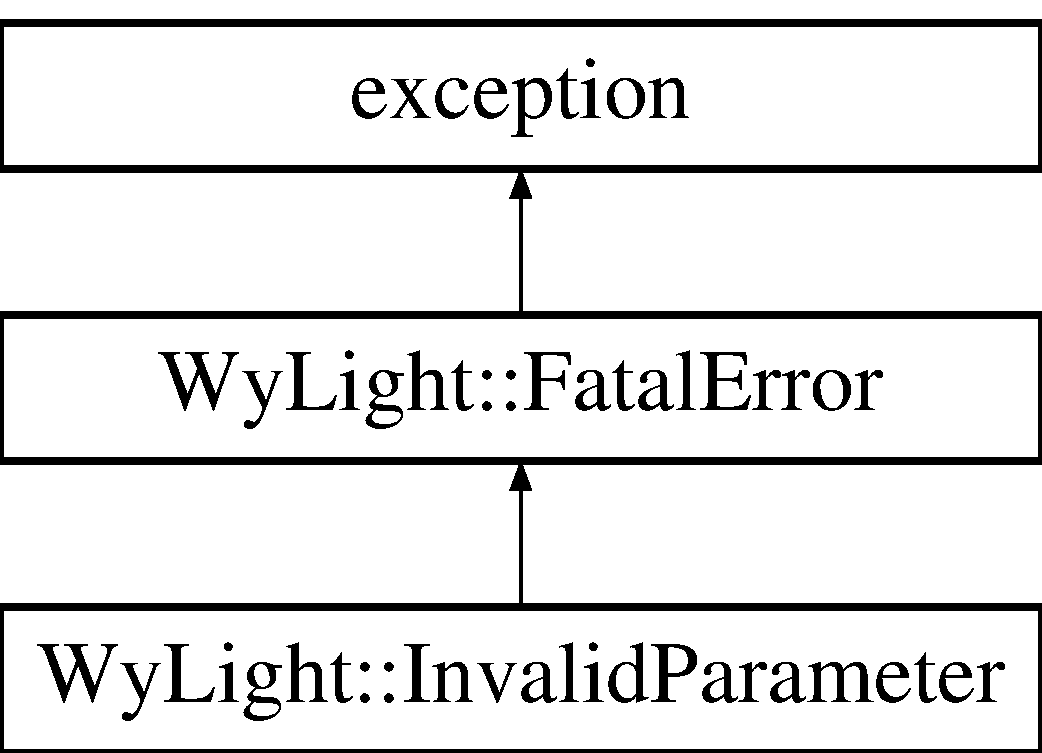
\includegraphics[height=3.000000cm]{class_wy_light_1_1_invalid_parameter}
\end{center}
\end{figure}
\subsection*{Public Member Functions}
\begin{DoxyCompactItemize}
\item 
\hyperlink{class_wy_light_1_1_invalid_parameter_a52625733bfa36035b8f0d0bb89b6d101}{Invalid\-Parameter} (const std\-::string \&description)
\item 
virtual const char $\ast$ \hyperlink{class_wy_light_1_1_invalid_parameter_a3cfc3b57f7a18e051e72efcfb4a67deb}{Get\-Java\-Class\-Type} (void) const 
\end{DoxyCompactItemize}
\subsection*{Additional Inherited Members}


\subsection{Constructor \& Destructor Documentation}
\hypertarget{class_wy_light_1_1_invalid_parameter_a52625733bfa36035b8f0d0bb89b6d101}{\index{Wy\-Light\-::\-Invalid\-Parameter@{Wy\-Light\-::\-Invalid\-Parameter}!Invalid\-Parameter@{Invalid\-Parameter}}
\index{Invalid\-Parameter@{Invalid\-Parameter}!WyLight::InvalidParameter@{Wy\-Light\-::\-Invalid\-Parameter}}
\subsubsection[{Invalid\-Parameter}]{\setlength{\rightskip}{0pt plus 5cm}Wy\-Light\-::\-Invalid\-Parameter\-::\-Invalid\-Parameter (
\begin{DoxyParamCaption}
\item[{const std\-::string \&}]{description}
\end{DoxyParamCaption}
)\hspace{0.3cm}{\ttfamily [inline]}}}\label{class_wy_light_1_1_invalid_parameter_a52625733bfa36035b8f0d0bb89b6d101}


\subsection{Member Function Documentation}
\hypertarget{class_wy_light_1_1_invalid_parameter_a3cfc3b57f7a18e051e72efcfb4a67deb}{\index{Wy\-Light\-::\-Invalid\-Parameter@{Wy\-Light\-::\-Invalid\-Parameter}!Get\-Java\-Class\-Type@{Get\-Java\-Class\-Type}}
\index{Get\-Java\-Class\-Type@{Get\-Java\-Class\-Type}!WyLight::InvalidParameter@{Wy\-Light\-::\-Invalid\-Parameter}}
\subsubsection[{Get\-Java\-Class\-Type}]{\setlength{\rightskip}{0pt plus 5cm}virtual const char$\ast$ Wy\-Light\-::\-Invalid\-Parameter\-::\-Get\-Java\-Class\-Type (
\begin{DoxyParamCaption}
\item[{void}]{}
\end{DoxyParamCaption}
) const\hspace{0.3cm}{\ttfamily [inline]}, {\ttfamily [virtual]}}}\label{class_wy_light_1_1_invalid_parameter_a3cfc3b57f7a18e051e72efcfb4a67deb}


Reimplemented from \hyperlink{class_wy_light_1_1_fatal_error_aa74decc09fe8aafc15bfbe31f697987a}{Wy\-Light\-::\-Fatal\-Error}.



The documentation for this class was generated from the following file\-:\begin{DoxyCompactItemize}
\item 
library/\hyperlink{_wifly_control_exception_8h}{Wifly\-Control\-Exception.\-h}\end{DoxyCompactItemize}

\hypertarget{struct_wy_light_1_1_ipv4_addr}{\section{Wy\-Light\-:\-:Ipv4\-Addr Struct Reference}
\label{struct_wy_light_1_1_ipv4_addr}\index{Wy\-Light\-::\-Ipv4\-Addr@{Wy\-Light\-::\-Ipv4\-Addr}}
}


{\ttfamily \#include $<$Client\-Socket.\-h$>$}

Inheritance diagram for Wy\-Light\-:\-:Ipv4\-Addr\-:\begin{figure}[H]
\begin{center}
\leavevmode
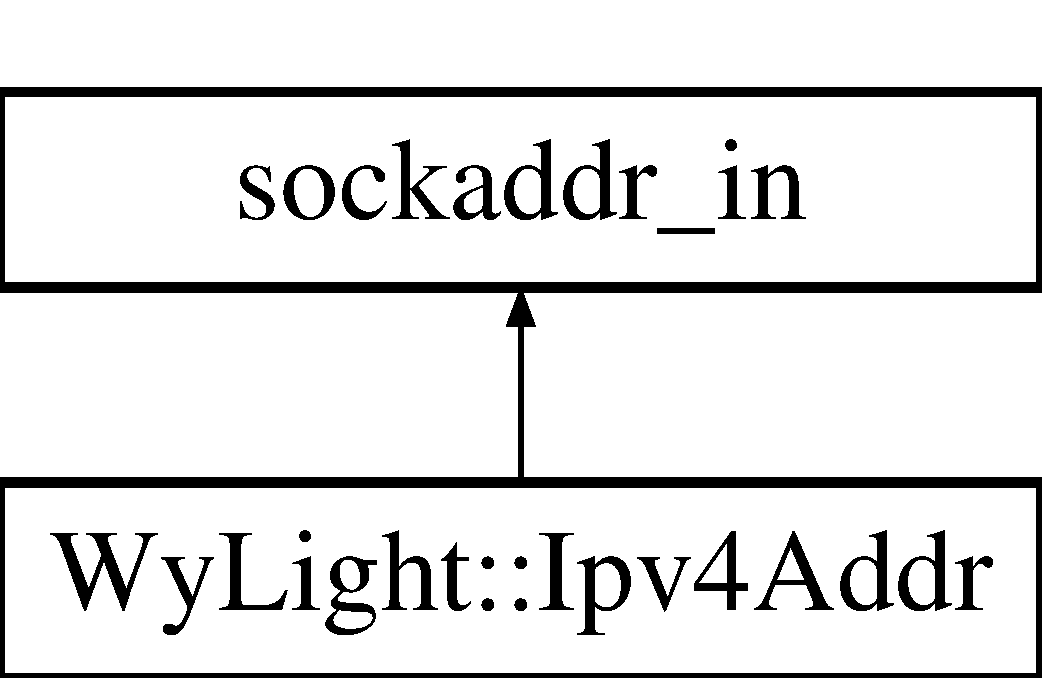
\includegraphics[height=2.000000cm]{struct_wy_light_1_1_ipv4_addr}
\end{center}
\end{figure}
\subsection*{Public Member Functions}
\begin{DoxyCompactItemize}
\item 
\hyperlink{struct_wy_light_1_1_ipv4_addr_a6ed8e919ab4ca060a98ef38c0b662262}{Ipv4\-Addr} (uint32\-\_\-t addr, uint16\-\_\-t port)
\end{DoxyCompactItemize}


\subsection{Detailed Description}
Helper class to simplify handling of sockaddr\-\_\-in 

\subsection{Constructor \& Destructor Documentation}
\hypertarget{struct_wy_light_1_1_ipv4_addr_a6ed8e919ab4ca060a98ef38c0b662262}{\index{Wy\-Light\-::\-Ipv4\-Addr@{Wy\-Light\-::\-Ipv4\-Addr}!Ipv4\-Addr@{Ipv4\-Addr}}
\index{Ipv4\-Addr@{Ipv4\-Addr}!WyLight::Ipv4Addr@{Wy\-Light\-::\-Ipv4\-Addr}}
\subsubsection[{Ipv4\-Addr}]{\setlength{\rightskip}{0pt plus 5cm}Wy\-Light\-::\-Ipv4\-Addr\-::\-Ipv4\-Addr (
\begin{DoxyParamCaption}
\item[{uint32\-\_\-t}]{addr, }
\item[{uint16\-\_\-t}]{port}
\end{DoxyParamCaption}
)\hspace{0.3cm}{\ttfamily [inline]}}}\label{struct_wy_light_1_1_ipv4_addr_a6ed8e919ab4ca060a98ef38c0b662262}


The documentation for this struct was generated from the following file\-:\begin{DoxyCompactItemize}
\item 
library/\hyperlink{_client_socket_8h}{Client\-Socket.\-h}\end{DoxyCompactItemize}

\hypertarget{class_wy_light_1_1_mask_buffer}{\section{Wy\-Light\-:\-:Mask\-Buffer Class Reference}
\label{class_wy_light_1_1_mask_buffer}\index{Wy\-Light\-::\-Mask\-Buffer@{Wy\-Light\-::\-Mask\-Buffer}}
}


{\ttfamily \#include $<$Mask\-Buffer.\-h$>$}

Inheritance diagram for Wy\-Light\-:\-:Mask\-Buffer\-:\begin{figure}[H]
\begin{center}
\leavevmode
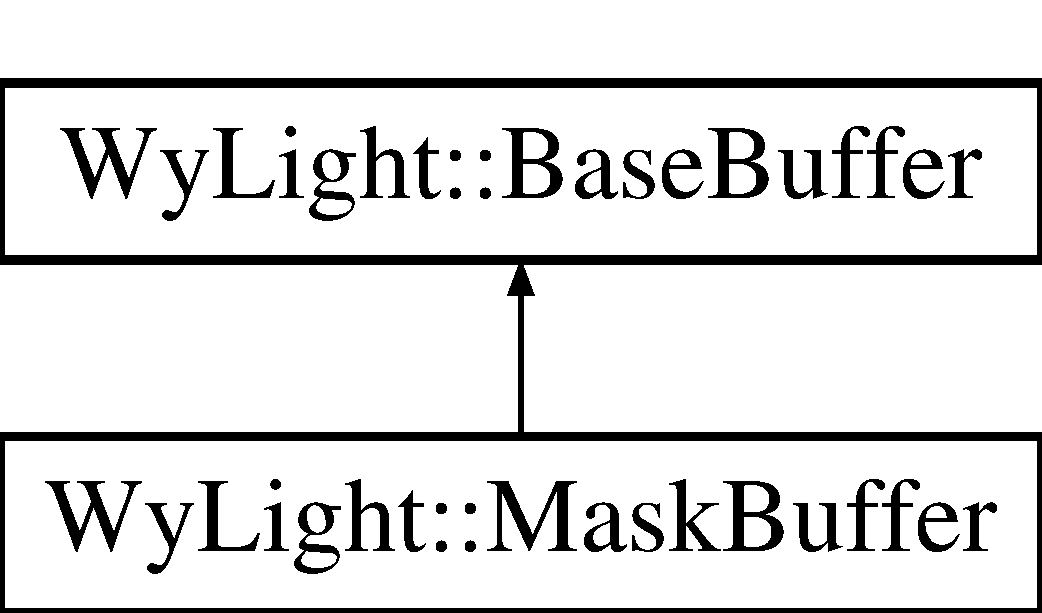
\includegraphics[height=2.000000cm]{class_wy_light_1_1_mask_buffer}
\end{center}
\end{figure}
\subsection*{Public Member Functions}
\begin{DoxyCompactItemize}
\item 
\hyperlink{class_wy_light_1_1_mask_buffer_a865583376a1ddb00632f1ecddd883759}{Mask\-Buffer} (size\-\_\-t capacity)
\item 
void \hyperlink{class_wy_light_1_1_mask_buffer_a6abd197d4d7fe655fdb1c6efdb8ebb71}{Mask} (const uint8\-\_\-t $\ast$p\-Input, const uint8\-\_\-t $\ast$const p\-Input\-End, const bool crc\-In\-Little\-Endian=true)
\end{DoxyCompactItemize}
\subsection*{Additional Inherited Members}


\subsection{Constructor \& Destructor Documentation}
\hypertarget{class_wy_light_1_1_mask_buffer_a865583376a1ddb00632f1ecddd883759}{\index{Wy\-Light\-::\-Mask\-Buffer@{Wy\-Light\-::\-Mask\-Buffer}!Mask\-Buffer@{Mask\-Buffer}}
\index{Mask\-Buffer@{Mask\-Buffer}!WyLight::MaskBuffer@{Wy\-Light\-::\-Mask\-Buffer}}
\subsubsection[{Mask\-Buffer}]{\setlength{\rightskip}{0pt plus 5cm}Wy\-Light\-::\-Mask\-Buffer\-::\-Mask\-Buffer (
\begin{DoxyParamCaption}
\item[{size\-\_\-t}]{capacity}
\end{DoxyParamCaption}
)\hspace{0.3cm}{\ttfamily [inline]}}}\label{class_wy_light_1_1_mask_buffer_a865583376a1ddb00632f1ecddd883759}


\subsection{Member Function Documentation}
\hypertarget{class_wy_light_1_1_mask_buffer_a6abd197d4d7fe655fdb1c6efdb8ebb71}{\index{Wy\-Light\-::\-Mask\-Buffer@{Wy\-Light\-::\-Mask\-Buffer}!Mask@{Mask}}
\index{Mask@{Mask}!WyLight::MaskBuffer@{Wy\-Light\-::\-Mask\-Buffer}}
\subsubsection[{Mask}]{\setlength{\rightskip}{0pt plus 5cm}void Wy\-Light\-::\-Mask\-Buffer\-::\-Mask (
\begin{DoxyParamCaption}
\item[{const uint8\-\_\-t $\ast$}]{p\-Input, }
\item[{const uint8\-\_\-t $\ast$const}]{p\-Input\-End, }
\item[{const bool}]{crc\-In\-Little\-Endian = {\ttfamily true}}
\end{DoxyParamCaption}
)}}\label{class_wy_light_1_1_mask_buffer_a6abd197d4d7fe655fdb1c6efdb8ebb71}


The documentation for this class was generated from the following file\-:\begin{DoxyCompactItemize}
\item 
library/\hyperlink{_mask_buffer_8h}{Mask\-Buffer.\-h}\end{DoxyCompactItemize}

\hypertarget{class_wy_light_1_1_message_queue}{\section{Wy\-Light\-:\-:Message\-Queue$<$ T $>$ Class Template Reference}
\label{class_wy_light_1_1_message_queue}\index{Wy\-Light\-::\-Message\-Queue$<$ T $>$@{Wy\-Light\-::\-Message\-Queue$<$ T $>$}}
}


{\ttfamily \#include $<$Message\-Queue.\-h$>$}

\subsection*{Public Member Functions}
\begin{DoxyCompactItemize}
\item 
\hyperlink{class_wy_light_1_1_message_queue_aa116745b3c6a257e7a8149432b1ae612}{Message\-Queue} (void)
\item 
\hyperlink{class_wy_light_1_1_message_queue_a92bf2e25bbd0feceabb3bf21368a4696}{Message\-Queue} (\hyperlink{class_wy_light_1_1_message_queue}{Message\-Queue} const \&\&other)
\item 
void \hyperlink{class_wy_light_1_1_message_queue_abb19b5612cabae621cffbb85b11acbce}{push\-\_\-back} (const T \&\&message)
\item 
void \hyperlink{class_wy_light_1_1_message_queue_a70d00934df73199dafe469dcd2aa750c}{push\-\_\-front} (const T \&\&message)
\item 
void \hyperlink{class_wy_light_1_1_message_queue_a07807ffc11826fb293b95f56fa2a6952}{clear} (void)
\item 
void \hyperlink{class_wy_light_1_1_message_queue_afa0cc613fbaf294bab1834b97d159de8}{clear\-\_\-and\-\_\-push\-\_\-front} (const T \&\&message)
\item 
bool \hyperlink{class_wy_light_1_1_message_queue_a2195f869b08d83342ac21353aa510161}{empty} (void) const 
\item 
void \hyperlink{class_wy_light_1_1_message_queue_ad7293e8940ef5c4cb34e62bfd389e5bc}{set\-Message\-Limit} (size\-\_\-t limit)
\item 
T \hyperlink{class_wy_light_1_1_message_queue_a8d993b590e708be1c3bdfd30112bdaa6}{receive} (void)
\end{DoxyCompactItemize}


\subsection{Constructor \& Destructor Documentation}
\hypertarget{class_wy_light_1_1_message_queue_aa116745b3c6a257e7a8149432b1ae612}{\index{Wy\-Light\-::\-Message\-Queue@{Wy\-Light\-::\-Message\-Queue}!Message\-Queue@{Message\-Queue}}
\index{Message\-Queue@{Message\-Queue}!WyLight::MessageQueue@{Wy\-Light\-::\-Message\-Queue}}
\subsubsection[{Message\-Queue}]{\setlength{\rightskip}{0pt plus 5cm}template$<$typename T $>$ {\bf Wy\-Light\-::\-Message\-Queue}$<$ T $>$\-::{\bf Message\-Queue} (
\begin{DoxyParamCaption}
\item[{void}]{}
\end{DoxyParamCaption}
)\hspace{0.3cm}{\ttfamily [inline]}}}\label{class_wy_light_1_1_message_queue_aa116745b3c6a257e7a8149432b1ae612}
\hypertarget{class_wy_light_1_1_message_queue_a92bf2e25bbd0feceabb3bf21368a4696}{\index{Wy\-Light\-::\-Message\-Queue@{Wy\-Light\-::\-Message\-Queue}!Message\-Queue@{Message\-Queue}}
\index{Message\-Queue@{Message\-Queue}!WyLight::MessageQueue@{Wy\-Light\-::\-Message\-Queue}}
\subsubsection[{Message\-Queue}]{\setlength{\rightskip}{0pt plus 5cm}template$<$typename T $>$ {\bf Wy\-Light\-::\-Message\-Queue}$<$ T $>$\-::{\bf Message\-Queue} (
\begin{DoxyParamCaption}
\item[{{\bf Message\-Queue}$<$ T $>$ const \&\&}]{other}
\end{DoxyParamCaption}
)\hspace{0.3cm}{\ttfamily [inline]}}}\label{class_wy_light_1_1_message_queue_a92bf2e25bbd0feceabb3bf21368a4696}


\subsection{Member Function Documentation}
\hypertarget{class_wy_light_1_1_message_queue_a07807ffc11826fb293b95f56fa2a6952}{\index{Wy\-Light\-::\-Message\-Queue@{Wy\-Light\-::\-Message\-Queue}!clear@{clear}}
\index{clear@{clear}!WyLight::MessageQueue@{Wy\-Light\-::\-Message\-Queue}}
\subsubsection[{clear}]{\setlength{\rightskip}{0pt plus 5cm}template$<$typename T $>$ void {\bf Wy\-Light\-::\-Message\-Queue}$<$ T $>$\-::clear (
\begin{DoxyParamCaption}
\item[{void}]{}
\end{DoxyParamCaption}
)}}\label{class_wy_light_1_1_message_queue_a07807ffc11826fb293b95f56fa2a6952}
\hypertarget{class_wy_light_1_1_message_queue_afa0cc613fbaf294bab1834b97d159de8}{\index{Wy\-Light\-::\-Message\-Queue@{Wy\-Light\-::\-Message\-Queue}!clear\-\_\-and\-\_\-push\-\_\-front@{clear\-\_\-and\-\_\-push\-\_\-front}}
\index{clear\-\_\-and\-\_\-push\-\_\-front@{clear\-\_\-and\-\_\-push\-\_\-front}!WyLight::MessageQueue@{Wy\-Light\-::\-Message\-Queue}}
\subsubsection[{clear\-\_\-and\-\_\-push\-\_\-front}]{\setlength{\rightskip}{0pt plus 5cm}template$<$typename T $>$ void {\bf Wy\-Light\-::\-Message\-Queue}$<$ T $>$\-::clear\-\_\-and\-\_\-push\-\_\-front (
\begin{DoxyParamCaption}
\item[{const T \&\&}]{message}
\end{DoxyParamCaption}
)}}\label{class_wy_light_1_1_message_queue_afa0cc613fbaf294bab1834b97d159de8}
\hypertarget{class_wy_light_1_1_message_queue_a2195f869b08d83342ac21353aa510161}{\index{Wy\-Light\-::\-Message\-Queue@{Wy\-Light\-::\-Message\-Queue}!empty@{empty}}
\index{empty@{empty}!WyLight::MessageQueue@{Wy\-Light\-::\-Message\-Queue}}
\subsubsection[{empty}]{\setlength{\rightskip}{0pt plus 5cm}template$<$typename T $>$ bool {\bf Wy\-Light\-::\-Message\-Queue}$<$ T $>$\-::empty (
\begin{DoxyParamCaption}
\item[{void}]{}
\end{DoxyParamCaption}
) const}}\label{class_wy_light_1_1_message_queue_a2195f869b08d83342ac21353aa510161}
\hypertarget{class_wy_light_1_1_message_queue_abb19b5612cabae621cffbb85b11acbce}{\index{Wy\-Light\-::\-Message\-Queue@{Wy\-Light\-::\-Message\-Queue}!push\-\_\-back@{push\-\_\-back}}
\index{push\-\_\-back@{push\-\_\-back}!WyLight::MessageQueue@{Wy\-Light\-::\-Message\-Queue}}
\subsubsection[{push\-\_\-back}]{\setlength{\rightskip}{0pt plus 5cm}template$<$typename T $>$ void {\bf Wy\-Light\-::\-Message\-Queue}$<$ T $>$\-::push\-\_\-back (
\begin{DoxyParamCaption}
\item[{const T \&\&}]{message}
\end{DoxyParamCaption}
)}}\label{class_wy_light_1_1_message_queue_abb19b5612cabae621cffbb85b11acbce}
\hypertarget{class_wy_light_1_1_message_queue_a70d00934df73199dafe469dcd2aa750c}{\index{Wy\-Light\-::\-Message\-Queue@{Wy\-Light\-::\-Message\-Queue}!push\-\_\-front@{push\-\_\-front}}
\index{push\-\_\-front@{push\-\_\-front}!WyLight::MessageQueue@{Wy\-Light\-::\-Message\-Queue}}
\subsubsection[{push\-\_\-front}]{\setlength{\rightskip}{0pt plus 5cm}template$<$typename T $>$ void {\bf Wy\-Light\-::\-Message\-Queue}$<$ T $>$\-::push\-\_\-front (
\begin{DoxyParamCaption}
\item[{const T \&\&}]{message}
\end{DoxyParamCaption}
)}}\label{class_wy_light_1_1_message_queue_a70d00934df73199dafe469dcd2aa750c}
\hypertarget{class_wy_light_1_1_message_queue_a8d993b590e708be1c3bdfd30112bdaa6}{\index{Wy\-Light\-::\-Message\-Queue@{Wy\-Light\-::\-Message\-Queue}!receive@{receive}}
\index{receive@{receive}!WyLight::MessageQueue@{Wy\-Light\-::\-Message\-Queue}}
\subsubsection[{receive}]{\setlength{\rightskip}{0pt plus 5cm}template$<$typename T $>$ T {\bf Wy\-Light\-::\-Message\-Queue}$<$ T $>$\-::receive (
\begin{DoxyParamCaption}
\item[{void}]{}
\end{DoxyParamCaption}
)}}\label{class_wy_light_1_1_message_queue_a8d993b590e708be1c3bdfd30112bdaa6}
\hypertarget{class_wy_light_1_1_message_queue_ad7293e8940ef5c4cb34e62bfd389e5bc}{\index{Wy\-Light\-::\-Message\-Queue@{Wy\-Light\-::\-Message\-Queue}!set\-Message\-Limit@{set\-Message\-Limit}}
\index{set\-Message\-Limit@{set\-Message\-Limit}!WyLight::MessageQueue@{Wy\-Light\-::\-Message\-Queue}}
\subsubsection[{set\-Message\-Limit}]{\setlength{\rightskip}{0pt plus 5cm}template$<$typename T $>$ void {\bf Wy\-Light\-::\-Message\-Queue}$<$ T $>$\-::set\-Message\-Limit (
\begin{DoxyParamCaption}
\item[{size\-\_\-t}]{limit}
\end{DoxyParamCaption}
)\hspace{0.3cm}{\ttfamily [inline]}}}\label{class_wy_light_1_1_message_queue_ad7293e8940ef5c4cb34e62bfd389e5bc}


The documentation for this class was generated from the following file\-:\begin{DoxyCompactItemize}
\item 
library/\hyperlink{_message_queue_8h}{Message\-Queue.\-h}\end{DoxyCompactItemize}

\hypertarget{class_wy_light_1_1_rtc_response}{\section{Wy\-Light\-:\-:Rtc\-Response Class Reference}
\label{class_wy_light_1_1_rtc_response}\index{Wy\-Light\-::\-Rtc\-Response@{Wy\-Light\-::\-Rtc\-Response}}
}


{\ttfamily \#include $<$Fw\-Response.\-h$>$}

Inheritance diagram for Wy\-Light\-:\-:Rtc\-Response\-:\begin{figure}[H]
\begin{center}
\leavevmode
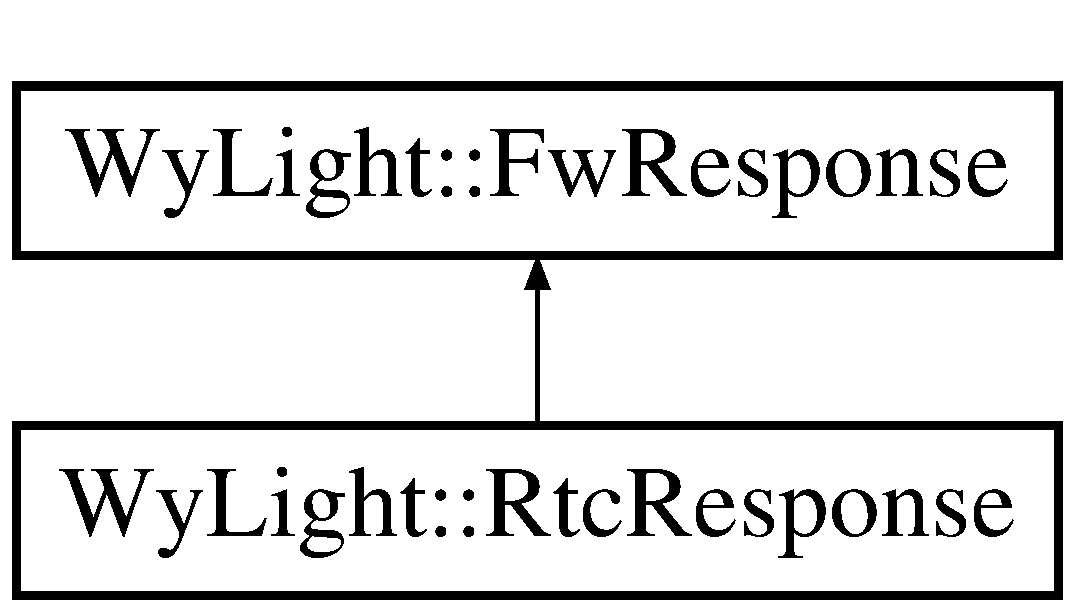
\includegraphics[height=2.000000cm]{class_wy_light_1_1_rtc_response}
\end{center}
\end{figure}
\subsection*{Public Member Functions}
\begin{DoxyCompactItemize}
\item 
\hyperlink{class_wy_light_1_1_rtc_response_a005721c3f86d547677851ff9f62dbb85}{Rtc\-Response} (void)
\item 
bool \hyperlink{class_wy_light_1_1_rtc_response_ab91706a872df459bba7c6dd8feab5e73}{Init} (response\-\_\-frame \&p\-Data, size\-\_\-t data\-Length)
\item 
struct tm \hyperlink{class_wy_light_1_1_rtc_response_a5789f86a808e71f53144eed137e3f9cf}{Get\-Real\-Time} (void) const 
\end{DoxyCompactItemize}


\subsection{Constructor \& Destructor Documentation}
\hypertarget{class_wy_light_1_1_rtc_response_a005721c3f86d547677851ff9f62dbb85}{\index{Wy\-Light\-::\-Rtc\-Response@{Wy\-Light\-::\-Rtc\-Response}!Rtc\-Response@{Rtc\-Response}}
\index{Rtc\-Response@{Rtc\-Response}!WyLight::RtcResponse@{Wy\-Light\-::\-Rtc\-Response}}
\subsubsection[{Rtc\-Response}]{\setlength{\rightskip}{0pt plus 5cm}Wy\-Light\-::\-Rtc\-Response\-::\-Rtc\-Response (
\begin{DoxyParamCaption}
\item[{void}]{}
\end{DoxyParamCaption}
)\hspace{0.3cm}{\ttfamily [inline]}}}\label{class_wy_light_1_1_rtc_response_a005721c3f86d547677851ff9f62dbb85}


\subsection{Member Function Documentation}
\hypertarget{class_wy_light_1_1_rtc_response_a5789f86a808e71f53144eed137e3f9cf}{\index{Wy\-Light\-::\-Rtc\-Response@{Wy\-Light\-::\-Rtc\-Response}!Get\-Real\-Time@{Get\-Real\-Time}}
\index{Get\-Real\-Time@{Get\-Real\-Time}!WyLight::RtcResponse@{Wy\-Light\-::\-Rtc\-Response}}
\subsubsection[{Get\-Real\-Time}]{\setlength{\rightskip}{0pt plus 5cm}struct tm Wy\-Light\-::\-Rtc\-Response\-::\-Get\-Real\-Time (
\begin{DoxyParamCaption}
\item[{void}]{}
\end{DoxyParamCaption}
) const\hspace{0.3cm}{\ttfamily [inline]}, {\ttfamily [read]}}}\label{class_wy_light_1_1_rtc_response_a5789f86a808e71f53144eed137e3f9cf}
\hypertarget{class_wy_light_1_1_rtc_response_ab91706a872df459bba7c6dd8feab5e73}{\index{Wy\-Light\-::\-Rtc\-Response@{Wy\-Light\-::\-Rtc\-Response}!Init@{Init}}
\index{Init@{Init}!WyLight::RtcResponse@{Wy\-Light\-::\-Rtc\-Response}}
\subsubsection[{Init}]{\setlength{\rightskip}{0pt plus 5cm}bool Wy\-Light\-::\-Rtc\-Response\-::\-Init (
\begin{DoxyParamCaption}
\item[{response\-\_\-frame \&}]{p\-Data, }
\item[{size\-\_\-t}]{data\-Length}
\end{DoxyParamCaption}
)\hspace{0.3cm}{\ttfamily [inline]}, {\ttfamily [virtual]}}}\label{class_wy_light_1_1_rtc_response_ab91706a872df459bba7c6dd8feab5e73}


Reimplemented from \hyperlink{class_wy_light_1_1_fw_response_aef349b4a6dd0f34c89ed8bcc8c512a55}{Wy\-Light\-::\-Fw\-Response}.



The documentation for this class was generated from the following file\-:\begin{DoxyCompactItemize}
\item 
library/\hyperlink{_fw_response_8h}{Fw\-Response.\-h}\end{DoxyCompactItemize}

\hypertarget{class_wy_light_1_1_script}{\section{Wy\-Light\-:\-:Script Class Reference}
\label{class_wy_light_1_1_script}\index{Wy\-Light\-::\-Script@{Wy\-Light\-::\-Script}}
}


{\ttfamily \#include $<$Script.\-h$>$}

Inheritance diagram for Wy\-Light\-:\-:Script\-:\begin{figure}[H]
\begin{center}
\leavevmode
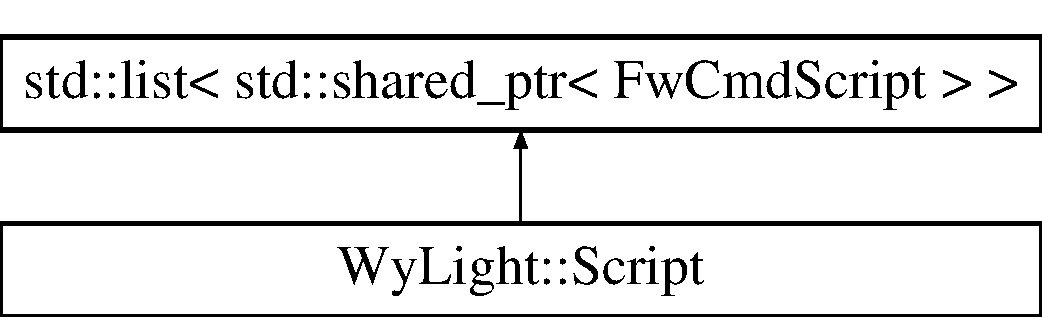
\includegraphics[height=2.000000cm]{class_wy_light_1_1_script}
\end{center}
\end{figure}
\subsection*{Public Member Functions}
\begin{DoxyCompactItemize}
\item 
\hyperlink{class_wy_light_1_1_script_a118aa641ff504296358639f105f2a449}{Script} (const std\-::string \&filename)
\item 
\hyperlink{class_wy_light_1_1_script_a9a6123b341e1b89fadae124f39f3a5c6}{$\sim$\-Script} (void)
\item 
bool \hyperlink{class_wy_light_1_1_script_afe14e21b96af672eed7fd8e10cba17ec}{operator==} (const \hyperlink{class_wy_light_1_1_script}{Script} \&ref) const 
\item 
{\footnotesize template$<$typename T $>$ }\\void \hyperlink{class_wy_light_1_1_script_af7fffcdda2a17b0e95aff472d558eb55}{emplace\-\_\-back} (T \&\&t)
\item 
{\footnotesize template$<$typename T $>$ }\\void \hyperlink{class_wy_light_1_1_script_ae9281ecb2099821ff0c5420590205676}{emplace\-\_\-front} (T \&\&t)
\end{DoxyCompactItemize}
\subsection*{Static Public Member Functions}
\begin{DoxyCompactItemize}
\item 
static void \hyperlink{class_wy_light_1_1_script_a3f1f1dc5f3c66572ba32ddb2c30c92a7}{deserialize} (const std\-::string \&filename, \hyperlink{class_wy_light_1_1_script}{Script} \&new\-Script)
\item 
static void \hyperlink{class_wy_light_1_1_script_a9d9ea9b2dc8642321f6d5f39cab82870}{serialize} (const std\-::string \&filename, const \hyperlink{class_wy_light_1_1_script}{Script} \&new\-Script)
\end{DoxyCompactItemize}


\subsection{Constructor \& Destructor Documentation}
\hypertarget{class_wy_light_1_1_script_a118aa641ff504296358639f105f2a449}{\index{Wy\-Light\-::\-Script@{Wy\-Light\-::\-Script}!Script@{Script}}
\index{Script@{Script}!WyLight::Script@{Wy\-Light\-::\-Script}}
\subsubsection[{Script}]{\setlength{\rightskip}{0pt plus 5cm}Wy\-Light\-::\-Script\-::\-Script (
\begin{DoxyParamCaption}
\item[{const std\-::string \&}]{filename}
\end{DoxyParamCaption}
)}}\label{class_wy_light_1_1_script_a118aa641ff504296358639f105f2a449}
\hypertarget{class_wy_light_1_1_script_a9a6123b341e1b89fadae124f39f3a5c6}{\index{Wy\-Light\-::\-Script@{Wy\-Light\-::\-Script}!$\sim$\-Script@{$\sim$\-Script}}
\index{$\sim$\-Script@{$\sim$\-Script}!WyLight::Script@{Wy\-Light\-::\-Script}}
\subsubsection[{$\sim$\-Script}]{\setlength{\rightskip}{0pt plus 5cm}Wy\-Light\-::\-Script\-::$\sim$\-Script (
\begin{DoxyParamCaption}
\item[{void}]{}
\end{DoxyParamCaption}
)}}\label{class_wy_light_1_1_script_a9a6123b341e1b89fadae124f39f3a5c6}


\subsection{Member Function Documentation}
\hypertarget{class_wy_light_1_1_script_a3f1f1dc5f3c66572ba32ddb2c30c92a7}{\index{Wy\-Light\-::\-Script@{Wy\-Light\-::\-Script}!deserialize@{deserialize}}
\index{deserialize@{deserialize}!WyLight::Script@{Wy\-Light\-::\-Script}}
\subsubsection[{deserialize}]{\setlength{\rightskip}{0pt plus 5cm}static void Wy\-Light\-::\-Script\-::deserialize (
\begin{DoxyParamCaption}
\item[{const std\-::string \&}]{filename, }
\item[{{\bf Script} \&}]{new\-Script}
\end{DoxyParamCaption}
)\hspace{0.3cm}{\ttfamily [static]}}}\label{class_wy_light_1_1_script_a3f1f1dc5f3c66572ba32ddb2c30c92a7}
\hypertarget{class_wy_light_1_1_script_af7fffcdda2a17b0e95aff472d558eb55}{\index{Wy\-Light\-::\-Script@{Wy\-Light\-::\-Script}!emplace\-\_\-back@{emplace\-\_\-back}}
\index{emplace\-\_\-back@{emplace\-\_\-back}!WyLight::Script@{Wy\-Light\-::\-Script}}
\subsubsection[{emplace\-\_\-back}]{\setlength{\rightskip}{0pt plus 5cm}template$<$typename T $>$ void Wy\-Light\-::\-Script\-::emplace\-\_\-back (
\begin{DoxyParamCaption}
\item[{T \&\&}]{t}
\end{DoxyParamCaption}
)\hspace{0.3cm}{\ttfamily [inline]}}}\label{class_wy_light_1_1_script_af7fffcdda2a17b0e95aff472d558eb55}
\hypertarget{class_wy_light_1_1_script_ae9281ecb2099821ff0c5420590205676}{\index{Wy\-Light\-::\-Script@{Wy\-Light\-::\-Script}!emplace\-\_\-front@{emplace\-\_\-front}}
\index{emplace\-\_\-front@{emplace\-\_\-front}!WyLight::Script@{Wy\-Light\-::\-Script}}
\subsubsection[{emplace\-\_\-front}]{\setlength{\rightskip}{0pt plus 5cm}template$<$typename T $>$ void Wy\-Light\-::\-Script\-::emplace\-\_\-front (
\begin{DoxyParamCaption}
\item[{T \&\&}]{t}
\end{DoxyParamCaption}
)\hspace{0.3cm}{\ttfamily [inline]}}}\label{class_wy_light_1_1_script_ae9281ecb2099821ff0c5420590205676}
\hypertarget{class_wy_light_1_1_script_afe14e21b96af672eed7fd8e10cba17ec}{\index{Wy\-Light\-::\-Script@{Wy\-Light\-::\-Script}!operator==@{operator==}}
\index{operator==@{operator==}!WyLight::Script@{Wy\-Light\-::\-Script}}
\subsubsection[{operator==}]{\setlength{\rightskip}{0pt plus 5cm}bool Wy\-Light\-::\-Script\-::operator== (
\begin{DoxyParamCaption}
\item[{const {\bf Script} \&}]{ref}
\end{DoxyParamCaption}
) const}}\label{class_wy_light_1_1_script_afe14e21b96af672eed7fd8e10cba17ec}
\hypertarget{class_wy_light_1_1_script_a9d9ea9b2dc8642321f6d5f39cab82870}{\index{Wy\-Light\-::\-Script@{Wy\-Light\-::\-Script}!serialize@{serialize}}
\index{serialize@{serialize}!WyLight::Script@{Wy\-Light\-::\-Script}}
\subsubsection[{serialize}]{\setlength{\rightskip}{0pt plus 5cm}static void Wy\-Light\-::\-Script\-::serialize (
\begin{DoxyParamCaption}
\item[{const std\-::string \&}]{filename, }
\item[{const {\bf Script} \&}]{new\-Script}
\end{DoxyParamCaption}
)\hspace{0.3cm}{\ttfamily [static]}}}\label{class_wy_light_1_1_script_a9d9ea9b2dc8642321f6d5f39cab82870}


The documentation for this class was generated from the following file\-:\begin{DoxyCompactItemize}
\item 
library/\hyperlink{_script_8h}{Script.\-h}\end{DoxyCompactItemize}

\hypertarget{class_wy_light_1_1_script_buffer_full}{\section{Wy\-Light\-:\-:Script\-Buffer\-Full Class Reference}
\label{class_wy_light_1_1_script_buffer_full}\index{Wy\-Light\-::\-Script\-Buffer\-Full@{Wy\-Light\-::\-Script\-Buffer\-Full}}
}


{\ttfamily \#include $<$Wifly\-Control\-Exception.\-h$>$}

Inheritance diagram for Wy\-Light\-:\-:Script\-Buffer\-Full\-:\begin{figure}[H]
\begin{center}
\leavevmode
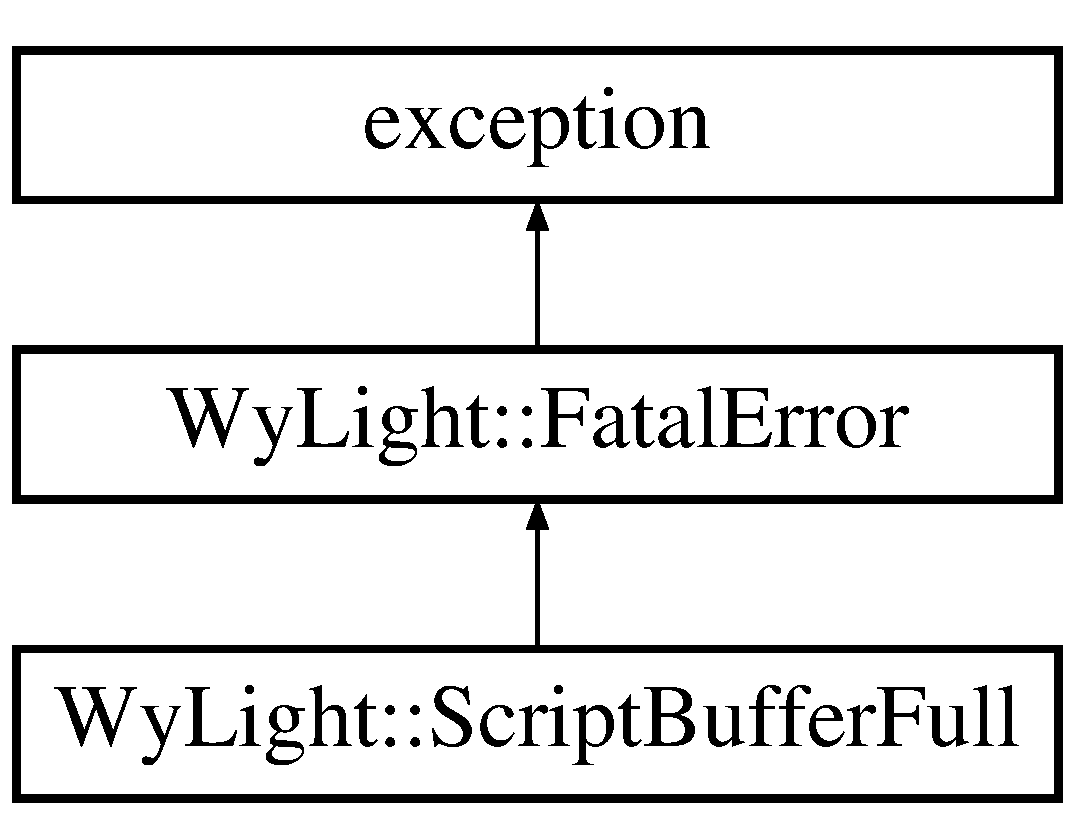
\includegraphics[height=3.000000cm]{class_wy_light_1_1_script_buffer_full}
\end{center}
\end{figure}
\subsection*{Public Member Functions}
\begin{DoxyCompactItemize}
\item 
\hyperlink{class_wy_light_1_1_script_buffer_full_adaeb5b2bff2bcc4500237fc12eaa634b}{Script\-Buffer\-Full} (void)
\item 
virtual const char $\ast$ \hyperlink{class_wy_light_1_1_script_buffer_full_ac228a7696643e89e4a571347bc9dda7d}{Get\-Java\-Class\-Type} (void) const 
\end{DoxyCompactItemize}
\subsection*{Additional Inherited Members}


\subsection{Constructor \& Destructor Documentation}
\hypertarget{class_wy_light_1_1_script_buffer_full_adaeb5b2bff2bcc4500237fc12eaa634b}{\index{Wy\-Light\-::\-Script\-Buffer\-Full@{Wy\-Light\-::\-Script\-Buffer\-Full}!Script\-Buffer\-Full@{Script\-Buffer\-Full}}
\index{Script\-Buffer\-Full@{Script\-Buffer\-Full}!WyLight::ScriptBufferFull@{Wy\-Light\-::\-Script\-Buffer\-Full}}
\subsubsection[{Script\-Buffer\-Full}]{\setlength{\rightskip}{0pt plus 5cm}Wy\-Light\-::\-Script\-Buffer\-Full\-::\-Script\-Buffer\-Full (
\begin{DoxyParamCaption}
\item[{void}]{}
\end{DoxyParamCaption}
)\hspace{0.3cm}{\ttfamily [inline]}}}\label{class_wy_light_1_1_script_buffer_full_adaeb5b2bff2bcc4500237fc12eaa634b}


\subsection{Member Function Documentation}
\hypertarget{class_wy_light_1_1_script_buffer_full_ac228a7696643e89e4a571347bc9dda7d}{\index{Wy\-Light\-::\-Script\-Buffer\-Full@{Wy\-Light\-::\-Script\-Buffer\-Full}!Get\-Java\-Class\-Type@{Get\-Java\-Class\-Type}}
\index{Get\-Java\-Class\-Type@{Get\-Java\-Class\-Type}!WyLight::ScriptBufferFull@{Wy\-Light\-::\-Script\-Buffer\-Full}}
\subsubsection[{Get\-Java\-Class\-Type}]{\setlength{\rightskip}{0pt plus 5cm}virtual const char$\ast$ Wy\-Light\-::\-Script\-Buffer\-Full\-::\-Get\-Java\-Class\-Type (
\begin{DoxyParamCaption}
\item[{void}]{}
\end{DoxyParamCaption}
) const\hspace{0.3cm}{\ttfamily [inline]}, {\ttfamily [virtual]}}}\label{class_wy_light_1_1_script_buffer_full_ac228a7696643e89e4a571347bc9dda7d}


Reimplemented from \hyperlink{class_wy_light_1_1_fatal_error_aa74decc09fe8aafc15bfbe31f697987a}{Wy\-Light\-::\-Fatal\-Error}.



The documentation for this class was generated from the following file\-:\begin{DoxyCompactItemize}
\item 
library/\hyperlink{_wifly_control_exception_8h}{Wifly\-Control\-Exception.\-h}\end{DoxyCompactItemize}

\hypertarget{class_wy_light_1_1_tcp_socket}{\section{Wy\-Light\-:\-:Tcp\-Socket Class Reference}
\label{class_wy_light_1_1_tcp_socket}\index{Wy\-Light\-::\-Tcp\-Socket@{Wy\-Light\-::\-Tcp\-Socket}}
}


{\ttfamily \#include $<$Client\-Socket.\-h$>$}

Inheritance diagram for Wy\-Light\-:\-:Tcp\-Socket\-:\begin{figure}[H]
\begin{center}
\leavevmode
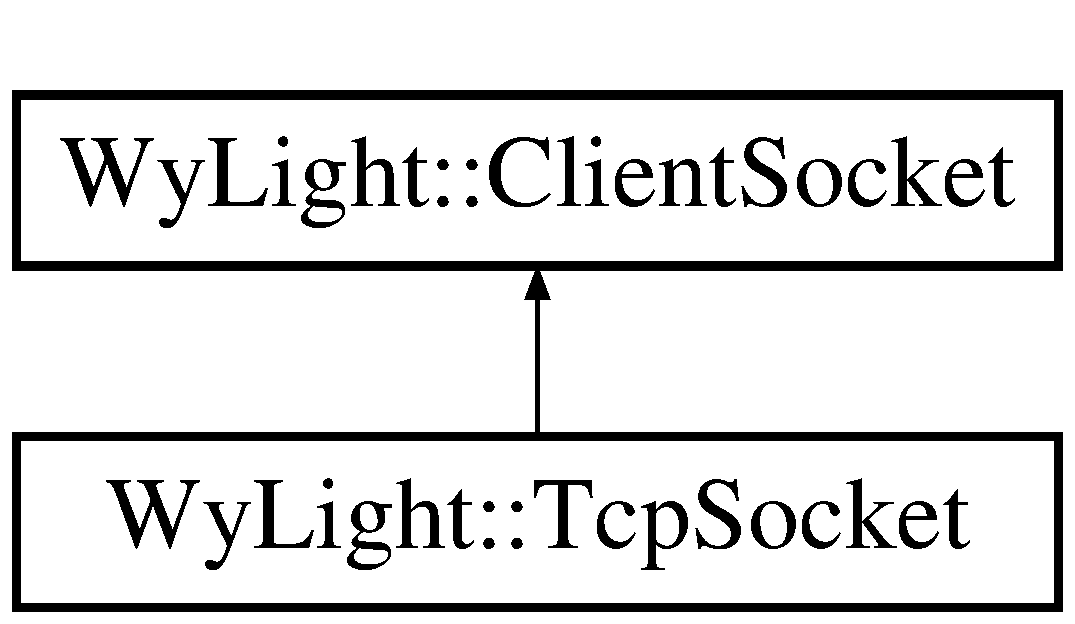
\includegraphics[height=2.000000cm]{class_wy_light_1_1_tcp_socket}
\end{center}
\end{figure}
\subsection*{Public Member Functions}
\begin{DoxyCompactItemize}
\item 
\hyperlink{class_wy_light_1_1_tcp_socket_a69045a3bf0b959b50b2b4d2a18ee06c1}{Tcp\-Socket} (uint32\-\_\-t Addr, uint16\-\_\-t port)  throw (\-Connection\-Lost, Fatal\-Error)
\item 
size\-\_\-t \hyperlink{class_wy_light_1_1_tcp_socket_aef83b055add4c47c4ab6b3395559ca27}{Recv} (uint8\-\_\-t $\ast$p\-Buffer, size\-\_\-t length, timeval $\ast$timeout=N\-U\-L\-L) const   throw (\-Fatal\-Error)
\item 
virtual size\-\_\-t \hyperlink{class_wy_light_1_1_tcp_socket_acd2ed7e05e7a8efc55b01e422d957857}{Send} (const uint8\-\_\-t $\ast$frame, size\-\_\-t length) const 
\end{DoxyCompactItemize}
\subsection*{Additional Inherited Members}


\subsection{Detailed Description}
Wrapper to make tcp socket handling more easy 

\subsection{Constructor \& Destructor Documentation}
\hypertarget{class_wy_light_1_1_tcp_socket_a69045a3bf0b959b50b2b4d2a18ee06c1}{\index{Wy\-Light\-::\-Tcp\-Socket@{Wy\-Light\-::\-Tcp\-Socket}!Tcp\-Socket@{Tcp\-Socket}}
\index{Tcp\-Socket@{Tcp\-Socket}!WyLight::TcpSocket@{Wy\-Light\-::\-Tcp\-Socket}}
\subsubsection[{Tcp\-Socket}]{\setlength{\rightskip}{0pt plus 5cm}Wy\-Light\-::\-Tcp\-Socket\-::\-Tcp\-Socket (
\begin{DoxyParamCaption}
\item[{uint32\-\_\-t}]{Addr, }
\item[{uint16\-\_\-t}]{port}
\end{DoxyParamCaption}
)  throw ({\bf Connection\-Lost}, {\bf Fatal\-Error})}}\label{class_wy_light_1_1_tcp_socket_a69045a3bf0b959b50b2b4d2a18ee06c1}

\begin{DoxyParams}{Parameters}
{\em Addr} & I\-Pv4 address in host byte order \\
\hline
{\em port} & I\-Pv4 port number in host byte order \\
\hline
\end{DoxyParams}

\begin{DoxyExceptions}{Exceptions}
{\em \hyperlink{class_wy_light_1_1_fatal_error}{Fatal\-Error}} & if the base class constructor fails\\
\hline
\end{DoxyExceptions}
\begin{DoxySeeAlso}{See Also}
\hyperlink{class_wy_light_1_1_client_socket_afe4f631abfffc996c24a8a55a9d5cea0}{Client\-Socket\-::\-Client\-Socket} 
\end{DoxySeeAlso}

\begin{DoxyExceptions}{Exceptions}
{\em \hyperlink{class_wy_light_1_1_connection_lost}{Connection\-Lost}} & if connect() fails on the internal socket \\
\hline
\end{DoxyExceptions}


\subsection{Member Function Documentation}
\hypertarget{class_wy_light_1_1_tcp_socket_aef83b055add4c47c4ab6b3395559ca27}{\index{Wy\-Light\-::\-Tcp\-Socket@{Wy\-Light\-::\-Tcp\-Socket}!Recv@{Recv}}
\index{Recv@{Recv}!WyLight::TcpSocket@{Wy\-Light\-::\-Tcp\-Socket}}
\subsubsection[{Recv}]{\setlength{\rightskip}{0pt plus 5cm}size\-\_\-t Wy\-Light\-::\-Tcp\-Socket\-::\-Recv (
\begin{DoxyParamCaption}
\item[{uint8\-\_\-t $\ast$}]{p\-Buffer, }
\item[{size\-\_\-t}]{length, }
\item[{timeval $\ast$}]{timeout = {\ttfamily NULL}}
\end{DoxyParamCaption}
) const  throw ({\bf Fatal\-Error})}}\label{class_wy_light_1_1_tcp_socket_aef83b055add4c47c4ab6b3395559ca27}
Receive data from the remote socket. 
\begin{DoxyParams}{Parameters}
{\em p\-Buffer} & to store the read data \\
\hline
{\em length} & size of the p\-Buffer \\
\hline
{\em timeout} & to wait for data, to block indefinitly use N\-U\-L\-L, which is default \\
\hline
\end{DoxyParams}
\begin{DoxyReturn}{Returns}
number of bytes read into $<$p\-Buffer$>$ 
\end{DoxyReturn}

\begin{DoxyExceptions}{Exceptions}
{\em \hyperlink{class_wy_light_1_1_fatal_error}{Fatal\-Error}} & if something very unexpected happens \\
\hline
\end{DoxyExceptions}
\hypertarget{class_wy_light_1_1_tcp_socket_acd2ed7e05e7a8efc55b01e422d957857}{\index{Wy\-Light\-::\-Tcp\-Socket@{Wy\-Light\-::\-Tcp\-Socket}!Send@{Send}}
\index{Send@{Send}!WyLight::TcpSocket@{Wy\-Light\-::\-Tcp\-Socket}}
\subsubsection[{Send}]{\setlength{\rightskip}{0pt plus 5cm}virtual size\-\_\-t Wy\-Light\-::\-Tcp\-Socket\-::\-Send (
\begin{DoxyParamCaption}
\item[{const uint8\-\_\-t $\ast$}]{frame, }
\item[{size\-\_\-t}]{length}
\end{DoxyParamCaption}
) const\hspace{0.3cm}{\ttfamily [virtual]}}}\label{class_wy_light_1_1_tcp_socket_acd2ed7e05e7a8efc55b01e422d957857}
\begin{DoxySeeAlso}{See Also}
\hyperlink{class_wy_light_1_1_client_socket_ab5ea6d042caa7f624015d514263ab6b5}{Client\-Socket\-::\-Send} 
\end{DoxySeeAlso}


Implements \hyperlink{class_wy_light_1_1_client_socket_ab5ea6d042caa7f624015d514263ab6b5}{Wy\-Light\-::\-Client\-Socket}.



The documentation for this class was generated from the following file\-:\begin{DoxyCompactItemize}
\item 
library/\hyperlink{_client_socket_8h}{Client\-Socket.\-h}\end{DoxyCompactItemize}

\hypertarget{class_wy_light_1_1_telnet_proxy}{\section{Wy\-Light\-:\-:Telnet\-Proxy Class Reference}
\label{class_wy_light_1_1_telnet_proxy}\index{Wy\-Light\-::\-Telnet\-Proxy@{Wy\-Light\-::\-Telnet\-Proxy}}
}


{\ttfamily \#include $<$Telnet\-Proxy.\-h$>$}

\subsection*{Public Member Functions}
\begin{DoxyCompactItemize}
\item 
\hyperlink{class_wy_light_1_1_telnet_proxy_a0d14c061adc13dd7f2f6d2b2bdbd700e}{Telnet\-Proxy} (const \hyperlink{class_wy_light_1_1_tcp_socket}{Tcp\-Socket} \&sock)
\item 
void \hyperlink{class_wy_light_1_1_telnet_proxy_ab438600992c7087b8bc8ec4248e4e9c1}{Clear\-Response} (void) const 
\item 
bool \hyperlink{class_wy_light_1_1_telnet_proxy_a21253eaad73040a3c23b4a234a1e4a7c}{Close} (bool do\-Save) const 
\item 
void \hyperlink{class_wy_light_1_1_telnet_proxy_ac4a01d35a096c4289467ae20c8e98909}{Recv\-String} (const std\-::string \&get\-Cmd, const std\-::string \&search\-Key, std\-::string \&result) const 
\item 
bool \hyperlink{class_wy_light_1_1_telnet_proxy_a296f650c20d7f577cef397cb5a558898}{Open} (void) const 
\item 
bool \hyperlink{class_wy_light_1_1_telnet_proxy_a5ac27544d8fde1b3c4c49a09ec2ce356}{Send} (const std\-::string \&telnet\-Message, const std\-::string \&expected\-Response=\hyperlink{_telnet_proxy_8h_a2139cfcd9b3c7af8c0246e72ca4ae807}{A\-O\-K}) const 
\item 
bool \hyperlink{class_wy_light_1_1_telnet_proxy_a2db92c2c87d880c90f7e48514e3bdb61}{Send\-String} (const std\-::string \&command, std\-::string value) const 
\item 
bool \hyperlink{class_wy_light_1_1_telnet_proxy_a92900b6d84df1080f9cb6cc5ae854a72}{Send\-Reboot\-Command} (void) const 
\item 
bool \hyperlink{class_wy_light_1_1_telnet_proxy_aae62f9bb24e292b0ad6afefbe2eafd77}{Perform\-Wifi\-Scan} (std\-::string \&result) const 
\item 
unsigned int \hyperlink{class_wy_light_1_1_telnet_proxy_a557df99e3968f7a86b0dbef55a6c6c72}{Compute\-Free\-Channel} (const std\-::string \&scan\-Results) const 
\item 
bool \hyperlink{class_wy_light_1_1_telnet_proxy_a0a454e69ec789b2d63faea69f480761c}{Change\-Wifi\-Channel} (const size\-\_\-t channel) const 
\end{DoxyCompactItemize}
\subsection*{Friends}
\begin{DoxyCompactItemize}
\item 
size\-\_\-t \hyperlink{class_wy_light_1_1_telnet_proxy_a436d76cf48d888700dddd5dc72c7bc56}{ut\-\_\-\-Telnet\-Proxy\-\_\-\-Recv} (void)
\item 
size\-\_\-t \hyperlink{class_wy_light_1_1_telnet_proxy_a899fd61cba9dec179f6a058b25c73cb7}{ut\-\_\-\-Telnet\-Proxy\-\_\-\-Recv\-String} (void)
\end{DoxyCompactItemize}


\subsection{Constructor \& Destructor Documentation}
\hypertarget{class_wy_light_1_1_telnet_proxy_a0d14c061adc13dd7f2f6d2b2bdbd700e}{\index{Wy\-Light\-::\-Telnet\-Proxy@{Wy\-Light\-::\-Telnet\-Proxy}!Telnet\-Proxy@{Telnet\-Proxy}}
\index{Telnet\-Proxy@{Telnet\-Proxy}!WyLight::TelnetProxy@{Wy\-Light\-::\-Telnet\-Proxy}}
\subsubsection[{Telnet\-Proxy}]{\setlength{\rightskip}{0pt plus 5cm}Wy\-Light\-::\-Telnet\-Proxy\-::\-Telnet\-Proxy (
\begin{DoxyParamCaption}
\item[{const {\bf Tcp\-Socket} \&}]{sock}
\end{DoxyParamCaption}
)}}\label{class_wy_light_1_1_telnet_proxy_a0d14c061adc13dd7f2f6d2b2bdbd700e}


\subsection{Member Function Documentation}
\hypertarget{class_wy_light_1_1_telnet_proxy_a0a454e69ec789b2d63faea69f480761c}{\index{Wy\-Light\-::\-Telnet\-Proxy@{Wy\-Light\-::\-Telnet\-Proxy}!Change\-Wifi\-Channel@{Change\-Wifi\-Channel}}
\index{Change\-Wifi\-Channel@{Change\-Wifi\-Channel}!WyLight::TelnetProxy@{Wy\-Light\-::\-Telnet\-Proxy}}
\subsubsection[{Change\-Wifi\-Channel}]{\setlength{\rightskip}{0pt plus 5cm}bool Wy\-Light\-::\-Telnet\-Proxy\-::\-Change\-Wifi\-Channel (
\begin{DoxyParamCaption}
\item[{const size\-\_\-t}]{channel}
\end{DoxyParamCaption}
) const}}\label{class_wy_light_1_1_telnet_proxy_a0a454e69ec789b2d63faea69f480761c}
\hypertarget{class_wy_light_1_1_telnet_proxy_ab438600992c7087b8bc8ec4248e4e9c1}{\index{Wy\-Light\-::\-Telnet\-Proxy@{Wy\-Light\-::\-Telnet\-Proxy}!Clear\-Response@{Clear\-Response}}
\index{Clear\-Response@{Clear\-Response}!WyLight::TelnetProxy@{Wy\-Light\-::\-Telnet\-Proxy}}
\subsubsection[{Clear\-Response}]{\setlength{\rightskip}{0pt plus 5cm}void Wy\-Light\-::\-Telnet\-Proxy\-::\-Clear\-Response (
\begin{DoxyParamCaption}
\item[{void}]{}
\end{DoxyParamCaption}
) const}}\label{class_wy_light_1_1_telnet_proxy_ab438600992c7087b8bc8ec4248e4e9c1}
\hypertarget{class_wy_light_1_1_telnet_proxy_a21253eaad73040a3c23b4a234a1e4a7c}{\index{Wy\-Light\-::\-Telnet\-Proxy@{Wy\-Light\-::\-Telnet\-Proxy}!Close@{Close}}
\index{Close@{Close}!WyLight::TelnetProxy@{Wy\-Light\-::\-Telnet\-Proxy}}
\subsubsection[{Close}]{\setlength{\rightskip}{0pt plus 5cm}bool Wy\-Light\-::\-Telnet\-Proxy\-::\-Close (
\begin{DoxyParamCaption}
\item[{bool}]{do\-Save}
\end{DoxyParamCaption}
) const}}\label{class_wy_light_1_1_telnet_proxy_a21253eaad73040a3c23b4a234a1e4a7c}
\hypertarget{class_wy_light_1_1_telnet_proxy_a557df99e3968f7a86b0dbef55a6c6c72}{\index{Wy\-Light\-::\-Telnet\-Proxy@{Wy\-Light\-::\-Telnet\-Proxy}!Compute\-Free\-Channel@{Compute\-Free\-Channel}}
\index{Compute\-Free\-Channel@{Compute\-Free\-Channel}!WyLight::TelnetProxy@{Wy\-Light\-::\-Telnet\-Proxy}}
\subsubsection[{Compute\-Free\-Channel}]{\setlength{\rightskip}{0pt plus 5cm}unsigned int Wy\-Light\-::\-Telnet\-Proxy\-::\-Compute\-Free\-Channel (
\begin{DoxyParamCaption}
\item[{const std\-::string \&}]{scan\-Results}
\end{DoxyParamCaption}
) const}}\label{class_wy_light_1_1_telnet_proxy_a557df99e3968f7a86b0dbef55a6c6c72}
\hypertarget{class_wy_light_1_1_telnet_proxy_a296f650c20d7f577cef397cb5a558898}{\index{Wy\-Light\-::\-Telnet\-Proxy@{Wy\-Light\-::\-Telnet\-Proxy}!Open@{Open}}
\index{Open@{Open}!WyLight::TelnetProxy@{Wy\-Light\-::\-Telnet\-Proxy}}
\subsubsection[{Open}]{\setlength{\rightskip}{0pt plus 5cm}bool Wy\-Light\-::\-Telnet\-Proxy\-::\-Open (
\begin{DoxyParamCaption}
\item[{void}]{}
\end{DoxyParamCaption}
) const}}\label{class_wy_light_1_1_telnet_proxy_a296f650c20d7f577cef397cb5a558898}
\hypertarget{class_wy_light_1_1_telnet_proxy_aae62f9bb24e292b0ad6afefbe2eafd77}{\index{Wy\-Light\-::\-Telnet\-Proxy@{Wy\-Light\-::\-Telnet\-Proxy}!Perform\-Wifi\-Scan@{Perform\-Wifi\-Scan}}
\index{Perform\-Wifi\-Scan@{Perform\-Wifi\-Scan}!WyLight::TelnetProxy@{Wy\-Light\-::\-Telnet\-Proxy}}
\subsubsection[{Perform\-Wifi\-Scan}]{\setlength{\rightskip}{0pt plus 5cm}bool Wy\-Light\-::\-Telnet\-Proxy\-::\-Perform\-Wifi\-Scan (
\begin{DoxyParamCaption}
\item[{std\-::string \&}]{result}
\end{DoxyParamCaption}
) const}}\label{class_wy_light_1_1_telnet_proxy_aae62f9bb24e292b0ad6afefbe2eafd77}
\hypertarget{class_wy_light_1_1_telnet_proxy_ac4a01d35a096c4289467ae20c8e98909}{\index{Wy\-Light\-::\-Telnet\-Proxy@{Wy\-Light\-::\-Telnet\-Proxy}!Recv\-String@{Recv\-String}}
\index{Recv\-String@{Recv\-String}!WyLight::TelnetProxy@{Wy\-Light\-::\-Telnet\-Proxy}}
\subsubsection[{Recv\-String}]{\setlength{\rightskip}{0pt plus 5cm}void Wy\-Light\-::\-Telnet\-Proxy\-::\-Recv\-String (
\begin{DoxyParamCaption}
\item[{const std\-::string \&}]{get\-Cmd, }
\item[{const std\-::string \&}]{search\-Key, }
\item[{std\-::string \&}]{result}
\end{DoxyParamCaption}
) const}}\label{class_wy_light_1_1_telnet_proxy_ac4a01d35a096c4289467ae20c8e98909}
\hypertarget{class_wy_light_1_1_telnet_proxy_a5ac27544d8fde1b3c4c49a09ec2ce356}{\index{Wy\-Light\-::\-Telnet\-Proxy@{Wy\-Light\-::\-Telnet\-Proxy}!Send@{Send}}
\index{Send@{Send}!WyLight::TelnetProxy@{Wy\-Light\-::\-Telnet\-Proxy}}
\subsubsection[{Send}]{\setlength{\rightskip}{0pt plus 5cm}bool Wy\-Light\-::\-Telnet\-Proxy\-::\-Send (
\begin{DoxyParamCaption}
\item[{const std\-::string \&}]{telnet\-Message, }
\item[{const std\-::string \&}]{expected\-Response = {\ttfamily {\bf A\-O\-K}}}
\end{DoxyParamCaption}
) const}}\label{class_wy_light_1_1_telnet_proxy_a5ac27544d8fde1b3c4c49a09ec2ce356}
\hypertarget{class_wy_light_1_1_telnet_proxy_a92900b6d84df1080f9cb6cc5ae854a72}{\index{Wy\-Light\-::\-Telnet\-Proxy@{Wy\-Light\-::\-Telnet\-Proxy}!Send\-Reboot\-Command@{Send\-Reboot\-Command}}
\index{Send\-Reboot\-Command@{Send\-Reboot\-Command}!WyLight::TelnetProxy@{Wy\-Light\-::\-Telnet\-Proxy}}
\subsubsection[{Send\-Reboot\-Command}]{\setlength{\rightskip}{0pt plus 5cm}bool Wy\-Light\-::\-Telnet\-Proxy\-::\-Send\-Reboot\-Command (
\begin{DoxyParamCaption}
\item[{void}]{}
\end{DoxyParamCaption}
) const}}\label{class_wy_light_1_1_telnet_proxy_a92900b6d84df1080f9cb6cc5ae854a72}
\hypertarget{class_wy_light_1_1_telnet_proxy_a2db92c2c87d880c90f7e48514e3bdb61}{\index{Wy\-Light\-::\-Telnet\-Proxy@{Wy\-Light\-::\-Telnet\-Proxy}!Send\-String@{Send\-String}}
\index{Send\-String@{Send\-String}!WyLight::TelnetProxy@{Wy\-Light\-::\-Telnet\-Proxy}}
\subsubsection[{Send\-String}]{\setlength{\rightskip}{0pt plus 5cm}bool Wy\-Light\-::\-Telnet\-Proxy\-::\-Send\-String (
\begin{DoxyParamCaption}
\item[{const std\-::string \&}]{command, }
\item[{std\-::string}]{value}
\end{DoxyParamCaption}
) const}}\label{class_wy_light_1_1_telnet_proxy_a2db92c2c87d880c90f7e48514e3bdb61}


\subsection{Friends And Related Function Documentation}
\hypertarget{class_wy_light_1_1_telnet_proxy_a436d76cf48d888700dddd5dc72c7bc56}{\index{Wy\-Light\-::\-Telnet\-Proxy@{Wy\-Light\-::\-Telnet\-Proxy}!ut\-\_\-\-Telnet\-Proxy\-\_\-\-Recv@{ut\-\_\-\-Telnet\-Proxy\-\_\-\-Recv}}
\index{ut\-\_\-\-Telnet\-Proxy\-\_\-\-Recv@{ut\-\_\-\-Telnet\-Proxy\-\_\-\-Recv}!WyLight::TelnetProxy@{Wy\-Light\-::\-Telnet\-Proxy}}
\subsubsection[{ut\-\_\-\-Telnet\-Proxy\-\_\-\-Recv}]{\setlength{\rightskip}{0pt plus 5cm}size\-\_\-t ut\-\_\-\-Telnet\-Proxy\-\_\-\-Recv (
\begin{DoxyParamCaption}
\item[{void}]{}
\end{DoxyParamCaption}
)\hspace{0.3cm}{\ttfamily [friend]}}}\label{class_wy_light_1_1_telnet_proxy_a436d76cf48d888700dddd5dc72c7bc56}
\hypertarget{class_wy_light_1_1_telnet_proxy_a899fd61cba9dec179f6a058b25c73cb7}{\index{Wy\-Light\-::\-Telnet\-Proxy@{Wy\-Light\-::\-Telnet\-Proxy}!ut\-\_\-\-Telnet\-Proxy\-\_\-\-Recv\-String@{ut\-\_\-\-Telnet\-Proxy\-\_\-\-Recv\-String}}
\index{ut\-\_\-\-Telnet\-Proxy\-\_\-\-Recv\-String@{ut\-\_\-\-Telnet\-Proxy\-\_\-\-Recv\-String}!WyLight::TelnetProxy@{Wy\-Light\-::\-Telnet\-Proxy}}
\subsubsection[{ut\-\_\-\-Telnet\-Proxy\-\_\-\-Recv\-String}]{\setlength{\rightskip}{0pt plus 5cm}size\-\_\-t ut\-\_\-\-Telnet\-Proxy\-\_\-\-Recv\-String (
\begin{DoxyParamCaption}
\item[{void}]{}
\end{DoxyParamCaption}
)\hspace{0.3cm}{\ttfamily [friend]}}}\label{class_wy_light_1_1_telnet_proxy_a899fd61cba9dec179f6a058b25c73cb7}


The documentation for this class was generated from the following file\-:\begin{DoxyCompactItemize}
\item 
library/\hyperlink{_telnet_proxy_8h}{Telnet\-Proxy.\-h}\end{DoxyCompactItemize}

\hypertarget{class_wy_light_1_1_tracebuffer_response}{\section{Wy\-Light\-:\-:Tracebuffer\-Response Class Reference}
\label{class_wy_light_1_1_tracebuffer_response}\index{Wy\-Light\-::\-Tracebuffer\-Response@{Wy\-Light\-::\-Tracebuffer\-Response}}
}


{\ttfamily \#include $<$Fw\-Response.\-h$>$}

Inheritance diagram for Wy\-Light\-:\-:Tracebuffer\-Response\-:\begin{figure}[H]
\begin{center}
\leavevmode
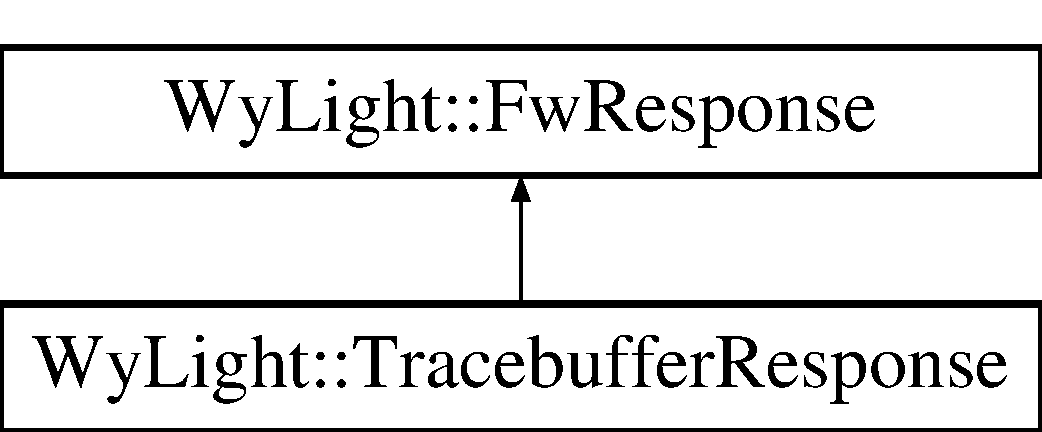
\includegraphics[height=2.000000cm]{class_wy_light_1_1_tracebuffer_response}
\end{center}
\end{figure}
\subsection*{Public Member Functions}
\begin{DoxyCompactItemize}
\item 
\hyperlink{class_wy_light_1_1_tracebuffer_response_ab8a2cdb129467f1fd155bfd9774b4e56}{Tracebuffer\-Response} (void)
\item 
bool \hyperlink{class_wy_light_1_1_tracebuffer_response_a07ea006c8b97ff7b2a6e3b2de6dbd45f}{Init} (response\-\_\-frame \&p\-Data, size\-\_\-t data\-Length)
\item 
std\-::string \hyperlink{class_wy_light_1_1_tracebuffer_response_a5fd5d2e19b21070606da3d5be3647665}{To\-String} (void) const 
\end{DoxyCompactItemize}
\subsection*{Friends}
\begin{DoxyCompactItemize}
\item 
std\-::ostream \& \hyperlink{class_wy_light_1_1_tracebuffer_response_a4ada06f1b6fe35635b6efdbbea164fd8}{operator$<$$<$} (std\-::ostream \&out, const \hyperlink{class_wy_light_1_1_tracebuffer_response}{Tracebuffer\-Response} \&ref)
\end{DoxyCompactItemize}


\subsection{Constructor \& Destructor Documentation}
\hypertarget{class_wy_light_1_1_tracebuffer_response_ab8a2cdb129467f1fd155bfd9774b4e56}{\index{Wy\-Light\-::\-Tracebuffer\-Response@{Wy\-Light\-::\-Tracebuffer\-Response}!Tracebuffer\-Response@{Tracebuffer\-Response}}
\index{Tracebuffer\-Response@{Tracebuffer\-Response}!WyLight::TracebufferResponse@{Wy\-Light\-::\-Tracebuffer\-Response}}
\subsubsection[{Tracebuffer\-Response}]{\setlength{\rightskip}{0pt plus 5cm}Wy\-Light\-::\-Tracebuffer\-Response\-::\-Tracebuffer\-Response (
\begin{DoxyParamCaption}
\item[{void}]{}
\end{DoxyParamCaption}
)\hspace{0.3cm}{\ttfamily [inline]}}}\label{class_wy_light_1_1_tracebuffer_response_ab8a2cdb129467f1fd155bfd9774b4e56}


\subsection{Member Function Documentation}
\hypertarget{class_wy_light_1_1_tracebuffer_response_a07ea006c8b97ff7b2a6e3b2de6dbd45f}{\index{Wy\-Light\-::\-Tracebuffer\-Response@{Wy\-Light\-::\-Tracebuffer\-Response}!Init@{Init}}
\index{Init@{Init}!WyLight::TracebufferResponse@{Wy\-Light\-::\-Tracebuffer\-Response}}
\subsubsection[{Init}]{\setlength{\rightskip}{0pt plus 5cm}bool Wy\-Light\-::\-Tracebuffer\-Response\-::\-Init (
\begin{DoxyParamCaption}
\item[{response\-\_\-frame \&}]{p\-Data, }
\item[{size\-\_\-t}]{data\-Length}
\end{DoxyParamCaption}
)\hspace{0.3cm}{\ttfamily [inline]}, {\ttfamily [virtual]}}}\label{class_wy_light_1_1_tracebuffer_response_a07ea006c8b97ff7b2a6e3b2de6dbd45f}


Reimplemented from \hyperlink{class_wy_light_1_1_fw_response_aef349b4a6dd0f34c89ed8bcc8c512a55}{Wy\-Light\-::\-Fw\-Response}.

\hypertarget{class_wy_light_1_1_tracebuffer_response_a5fd5d2e19b21070606da3d5be3647665}{\index{Wy\-Light\-::\-Tracebuffer\-Response@{Wy\-Light\-::\-Tracebuffer\-Response}!To\-String@{To\-String}}
\index{To\-String@{To\-String}!WyLight::TracebufferResponse@{Wy\-Light\-::\-Tracebuffer\-Response}}
\subsubsection[{To\-String}]{\setlength{\rightskip}{0pt plus 5cm}std\-::string Wy\-Light\-::\-Tracebuffer\-Response\-::\-To\-String (
\begin{DoxyParamCaption}
\item[{void}]{}
\end{DoxyParamCaption}
) const\hspace{0.3cm}{\ttfamily [inline]}}}\label{class_wy_light_1_1_tracebuffer_response_a5fd5d2e19b21070606da3d5be3647665}


\subsection{Friends And Related Function Documentation}
\hypertarget{class_wy_light_1_1_tracebuffer_response_a4ada06f1b6fe35635b6efdbbea164fd8}{\index{Wy\-Light\-::\-Tracebuffer\-Response@{Wy\-Light\-::\-Tracebuffer\-Response}!operator$<$$<$@{operator$<$$<$}}
\index{operator$<$$<$@{operator$<$$<$}!WyLight::TracebufferResponse@{Wy\-Light\-::\-Tracebuffer\-Response}}
\subsubsection[{operator$<$$<$}]{\setlength{\rightskip}{0pt plus 5cm}std\-::ostream\& operator$<$$<$ (
\begin{DoxyParamCaption}
\item[{std\-::ostream \&}]{out, }
\item[{const {\bf Tracebuffer\-Response} \&}]{ref}
\end{DoxyParamCaption}
)\hspace{0.3cm}{\ttfamily [friend]}}}\label{class_wy_light_1_1_tracebuffer_response_a4ada06f1b6fe35635b6efdbbea164fd8}


The documentation for this class was generated from the following file\-:\begin{DoxyCompactItemize}
\item 
library/\hyperlink{_fw_response_8h}{Fw\-Response.\-h}\end{DoxyCompactItemize}

\hypertarget{class_wy_light_1_1_udp_socket}{\section{Wy\-Light\-:\-:Udp\-Socket Class Reference}
\label{class_wy_light_1_1_udp_socket}\index{Wy\-Light\-::\-Udp\-Socket@{Wy\-Light\-::\-Udp\-Socket}}
}


{\ttfamily \#include $<$Client\-Socket.\-h$>$}

Inheritance diagram for Wy\-Light\-:\-:Udp\-Socket\-:\begin{figure}[H]
\begin{center}
\leavevmode
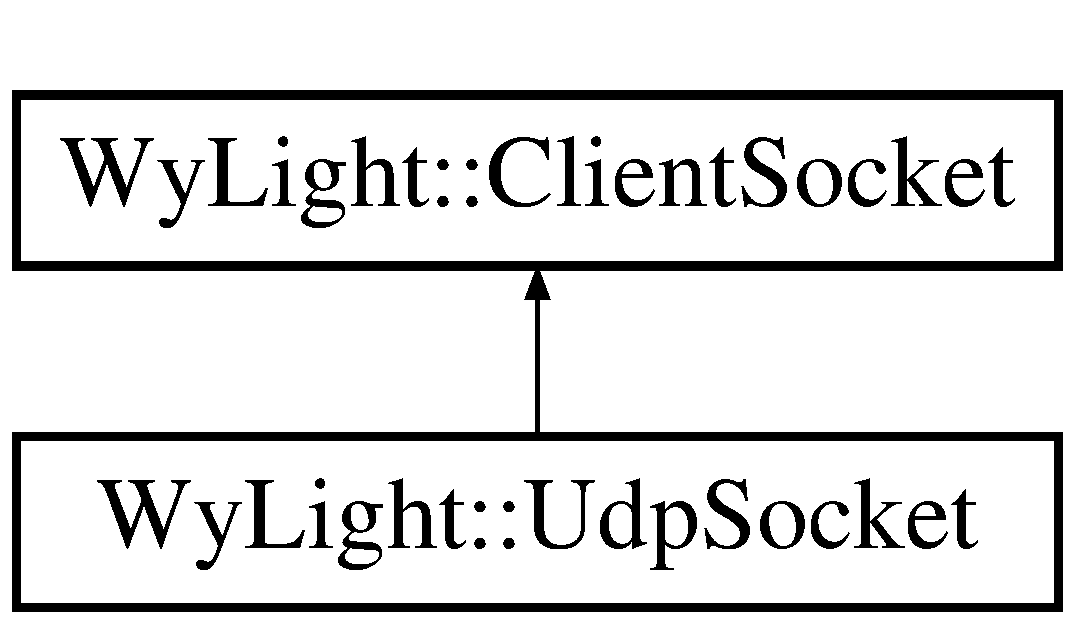
\includegraphics[height=2.000000cm]{class_wy_light_1_1_udp_socket}
\end{center}
\end{figure}
\subsection*{Public Member Functions}
\begin{DoxyCompactItemize}
\item 
\hyperlink{class_wy_light_1_1_udp_socket_adcf1f11b78b2485b475f3b040ff8f2d4}{Udp\-Socket} (uint32\-\_\-t addr, uint16\-\_\-t port, bool do\-Bind=true, int enable\-Broadcast=0)  throw (\-Fatal\-Error)
\item 
size\-\_\-t \hyperlink{class_wy_light_1_1_udp_socket_a937cb9beb6c957e0870228815e1d2cb4}{Recv\-From} (uint8\-\_\-t $\ast$p\-Buffer, size\-\_\-t length, timeval $\ast$timeout=N\-U\-L\-L, struct sockaddr $\ast$remote\-Addr=N\-U\-L\-L, socklen\-\_\-t $\ast$remote\-Addr\-Length=N\-U\-L\-L) const   throw (\-Fatal\-Error)
\item 
virtual size\-\_\-t \hyperlink{class_wy_light_1_1_udp_socket_aaba73a044c8aed0ef0c1e44ce46d88ca}{Send} (const uint8\-\_\-t $\ast$frame, size\-\_\-t length) const 
\end{DoxyCompactItemize}
\subsection*{Additional Inherited Members}


\subsection{Detailed Description}
Wrapper to make udp socket handling more easy 

\subsection{Constructor \& Destructor Documentation}
\hypertarget{class_wy_light_1_1_udp_socket_adcf1f11b78b2485b475f3b040ff8f2d4}{\index{Wy\-Light\-::\-Udp\-Socket@{Wy\-Light\-::\-Udp\-Socket}!Udp\-Socket@{Udp\-Socket}}
\index{Udp\-Socket@{Udp\-Socket}!WyLight::UdpSocket@{Wy\-Light\-::\-Udp\-Socket}}
\subsubsection[{Udp\-Socket}]{\setlength{\rightskip}{0pt plus 5cm}Wy\-Light\-::\-Udp\-Socket\-::\-Udp\-Socket (
\begin{DoxyParamCaption}
\item[{uint32\-\_\-t}]{addr, }
\item[{uint16\-\_\-t}]{port, }
\item[{bool}]{do\-Bind = {\ttfamily true}, }
\item[{int}]{enable\-Broadcast = {\ttfamily 0}}
\end{DoxyParamCaption}
)  throw ({\bf Fatal\-Error})}}\label{class_wy_light_1_1_udp_socket_adcf1f11b78b2485b475f3b040ff8f2d4}

\begin{DoxyParams}{Parameters}
{\em addr} & I\-Pv4 address in host byte order \\
\hline
{\em port} & I\-Pv4 port number in host byte order \\
\hline
{\em do\-Bind} & set to true to \\
\hline
{\em enable\-Broadcast} & use 1 to enable broadcast else set 0 (default) \\
\hline
\end{DoxyParams}

\begin{DoxyExceptions}{Exceptions}
{\em \hyperlink{class_wy_light_1_1_fatal_error}{Fatal\-Error}} & if the base class constructor fails \\
\hline
\end{DoxyExceptions}


\subsection{Member Function Documentation}
\hypertarget{class_wy_light_1_1_udp_socket_a937cb9beb6c957e0870228815e1d2cb4}{\index{Wy\-Light\-::\-Udp\-Socket@{Wy\-Light\-::\-Udp\-Socket}!Recv\-From@{Recv\-From}}
\index{Recv\-From@{Recv\-From}!WyLight::UdpSocket@{Wy\-Light\-::\-Udp\-Socket}}
\subsubsection[{Recv\-From}]{\setlength{\rightskip}{0pt plus 5cm}size\-\_\-t Wy\-Light\-::\-Udp\-Socket\-::\-Recv\-From (
\begin{DoxyParamCaption}
\item[{uint8\-\_\-t $\ast$}]{p\-Buffer, }
\item[{size\-\_\-t}]{length, }
\item[{timeval $\ast$}]{timeout = {\ttfamily NULL}, }
\item[{struct sockaddr $\ast$}]{remote\-Addr = {\ttfamily NULL}, }
\item[{socklen\-\_\-t $\ast$}]{remote\-Addr\-Length = {\ttfamily NULL}}
\end{DoxyParamCaption}
) const  throw ({\bf Fatal\-Error})}}\label{class_wy_light_1_1_udp_socket_a937cb9beb6c957e0870228815e1d2cb4}
Receive data from the remote socket. 
\begin{DoxyParams}{Parameters}
{\em p\-Buffer} & to store the read data \\
\hline
{\em length} & size of the p\-Buffer \\
\hline
{\em timeout} & to wait for data, to block indefinitly use N\-U\-L\-L, which is default \\
\hline
{\em remote\-Addr} & pointer to a struct where the senders address should be stored, this param is optional use N\-U\-L\-L to ignore it \\
\hline
{\em remote\-Addr\-Length} & size of the struct remote\-Addr is pointing to, after a successfull call with no N\-U\-L\-L pointers in remote\-Addr\-Length and remote\-Addr it will point to the size of the written remote\-Addr struct \\
\hline
\end{DoxyParams}
\begin{DoxyReturn}{Returns}
number of bytes read into $<$p\-Buffer$>$, 0 in case of a timeout 
\end{DoxyReturn}

\begin{DoxyExceptions}{Exceptions}
{\em \hyperlink{class_wy_light_1_1_fatal_error}{Fatal\-Error}} & if something very unexpected happens \\
\hline
\end{DoxyExceptions}
\hypertarget{class_wy_light_1_1_udp_socket_aaba73a044c8aed0ef0c1e44ce46d88ca}{\index{Wy\-Light\-::\-Udp\-Socket@{Wy\-Light\-::\-Udp\-Socket}!Send@{Send}}
\index{Send@{Send}!WyLight::UdpSocket@{Wy\-Light\-::\-Udp\-Socket}}
\subsubsection[{Send}]{\setlength{\rightskip}{0pt plus 5cm}virtual size\-\_\-t Wy\-Light\-::\-Udp\-Socket\-::\-Send (
\begin{DoxyParamCaption}
\item[{const uint8\-\_\-t $\ast$}]{frame, }
\item[{size\-\_\-t}]{length}
\end{DoxyParamCaption}
) const\hspace{0.3cm}{\ttfamily [virtual]}}}\label{class_wy_light_1_1_udp_socket_aaba73a044c8aed0ef0c1e44ce46d88ca}
Interface to send a data frame with a given length, you have to implement this function in child classes 

Implements \hyperlink{class_wy_light_1_1_client_socket_ab5ea6d042caa7f624015d514263ab6b5}{Wy\-Light\-::\-Client\-Socket}.



The documentation for this class was generated from the following file\-:\begin{DoxyCompactItemize}
\item 
library/\hyperlink{_client_socket_8h}{Client\-Socket.\-h}\end{DoxyCompactItemize}

\hypertarget{class_wy_light_1_1_unmask_buffer}{\section{Wy\-Light\-:\-:Unmask\-Buffer Class Reference}
\label{class_wy_light_1_1_unmask_buffer}\index{Wy\-Light\-::\-Unmask\-Buffer@{Wy\-Light\-::\-Unmask\-Buffer}}
}


{\ttfamily \#include $<$Mask\-Buffer.\-h$>$}

Inheritance diagram for Wy\-Light\-:\-:Unmask\-Buffer\-:\begin{figure}[H]
\begin{center}
\leavevmode
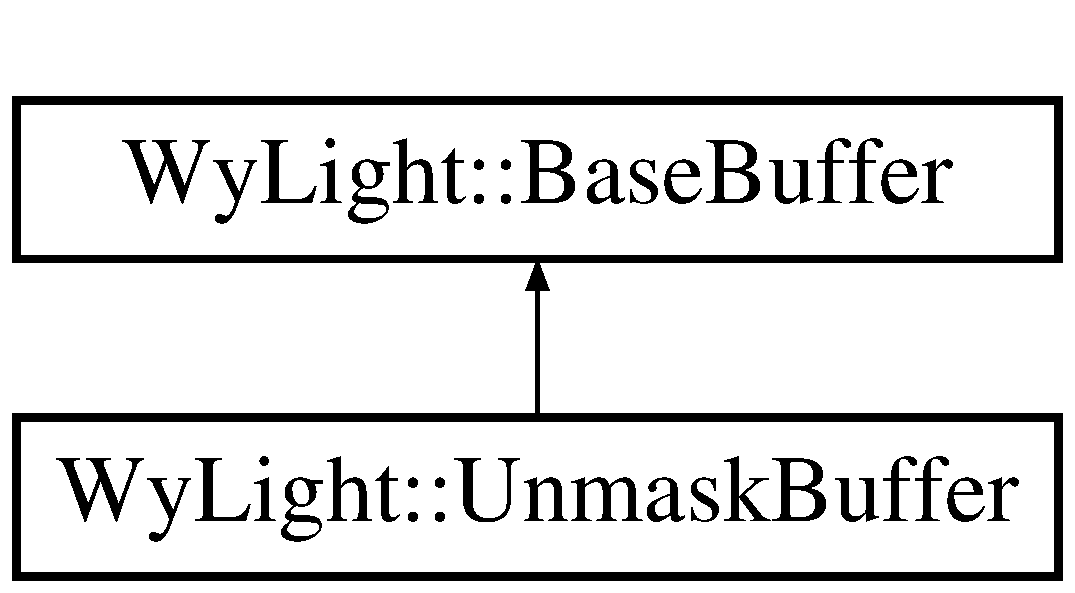
\includegraphics[height=2.000000cm]{class_wy_light_1_1_unmask_buffer}
\end{center}
\end{figure}
\subsection*{Public Member Functions}
\begin{DoxyCompactItemize}
\item 
\hyperlink{class_wy_light_1_1_unmask_buffer_a664016ab8306b9c72c01a8d57b2404b5}{Unmask\-Buffer} (size\-\_\-t capacity)
\item 
void \hyperlink{class_wy_light_1_1_unmask_buffer_a176ee14660b44137a8ce041c7e338b94}{Add} (uint8\-\_\-t new\-Byte)
\item 
void \hyperlink{class_wy_light_1_1_unmask_buffer_a0d535dd72bf7759dc780e1341f30a75f}{Clear} (void)
\item 
void \hyperlink{class_wy_light_1_1_unmask_buffer_a4ce5f97f46916275ddb5f919483acab6}{Check\-And\-Remove\-Crc} (bool crc\-In\-Little\-Endian)  throw (\-Fatal\-Error)
\item 
bool \hyperlink{class_wy_light_1_1_unmask_buffer_a8268033300f5f43ad9ccb2e806b84b44}{Unmask} (const uint8\-\_\-t $\ast$p\-Input, size\-\_\-t bytes\-Masked, bool check\-Crc, bool crc\-In\-Little\-Endian)
\end{DoxyCompactItemize}
\subsection*{Additional Inherited Members}


\subsection{Constructor \& Destructor Documentation}
\hypertarget{class_wy_light_1_1_unmask_buffer_a664016ab8306b9c72c01a8d57b2404b5}{\index{Wy\-Light\-::\-Unmask\-Buffer@{Wy\-Light\-::\-Unmask\-Buffer}!Unmask\-Buffer@{Unmask\-Buffer}}
\index{Unmask\-Buffer@{Unmask\-Buffer}!WyLight::UnmaskBuffer@{Wy\-Light\-::\-Unmask\-Buffer}}
\subsubsection[{Unmask\-Buffer}]{\setlength{\rightskip}{0pt plus 5cm}Wy\-Light\-::\-Unmask\-Buffer\-::\-Unmask\-Buffer (
\begin{DoxyParamCaption}
\item[{size\-\_\-t}]{capacity}
\end{DoxyParamCaption}
)\hspace{0.3cm}{\ttfamily [inline]}}}\label{class_wy_light_1_1_unmask_buffer_a664016ab8306b9c72c01a8d57b2404b5}


\subsection{Member Function Documentation}
\hypertarget{class_wy_light_1_1_unmask_buffer_a176ee14660b44137a8ce041c7e338b94}{\index{Wy\-Light\-::\-Unmask\-Buffer@{Wy\-Light\-::\-Unmask\-Buffer}!Add@{Add}}
\index{Add@{Add}!WyLight::UnmaskBuffer@{Wy\-Light\-::\-Unmask\-Buffer}}
\subsubsection[{Add}]{\setlength{\rightskip}{0pt plus 5cm}void Wy\-Light\-::\-Unmask\-Buffer\-::\-Add (
\begin{DoxyParamCaption}
\item[{uint8\-\_\-t}]{new\-Byte}
\end{DoxyParamCaption}
)}}\label{class_wy_light_1_1_unmask_buffer_a176ee14660b44137a8ce041c7e338b94}
\hypertarget{class_wy_light_1_1_unmask_buffer_a4ce5f97f46916275ddb5f919483acab6}{\index{Wy\-Light\-::\-Unmask\-Buffer@{Wy\-Light\-::\-Unmask\-Buffer}!Check\-And\-Remove\-Crc@{Check\-And\-Remove\-Crc}}
\index{Check\-And\-Remove\-Crc@{Check\-And\-Remove\-Crc}!WyLight::UnmaskBuffer@{Wy\-Light\-::\-Unmask\-Buffer}}
\subsubsection[{Check\-And\-Remove\-Crc}]{\setlength{\rightskip}{0pt plus 5cm}void Wy\-Light\-::\-Unmask\-Buffer\-::\-Check\-And\-Remove\-Crc (
\begin{DoxyParamCaption}
\item[{bool}]{crc\-In\-Little\-Endian}
\end{DoxyParamCaption}
)  throw ({\bf Fatal\-Error})}}\label{class_wy_light_1_1_unmask_buffer_a4ce5f97f46916275ddb5f919483acab6}
\hypertarget{class_wy_light_1_1_unmask_buffer_a0d535dd72bf7759dc780e1341f30a75f}{\index{Wy\-Light\-::\-Unmask\-Buffer@{Wy\-Light\-::\-Unmask\-Buffer}!Clear@{Clear}}
\index{Clear@{Clear}!WyLight::UnmaskBuffer@{Wy\-Light\-::\-Unmask\-Buffer}}
\subsubsection[{Clear}]{\setlength{\rightskip}{0pt plus 5cm}void Wy\-Light\-::\-Unmask\-Buffer\-::\-Clear (
\begin{DoxyParamCaption}
\item[{void}]{}
\end{DoxyParamCaption}
)\hspace{0.3cm}{\ttfamily [virtual]}}}\label{class_wy_light_1_1_unmask_buffer_a0d535dd72bf7759dc780e1341f30a75f}


Reimplemented from \hyperlink{class_wy_light_1_1_base_buffer_ad7c6538cc7136f71a96efe6d85c8ff8f}{Wy\-Light\-::\-Base\-Buffer}.

\hypertarget{class_wy_light_1_1_unmask_buffer_a8268033300f5f43ad9ccb2e806b84b44}{\index{Wy\-Light\-::\-Unmask\-Buffer@{Wy\-Light\-::\-Unmask\-Buffer}!Unmask@{Unmask}}
\index{Unmask@{Unmask}!WyLight::UnmaskBuffer@{Wy\-Light\-::\-Unmask\-Buffer}}
\subsubsection[{Unmask}]{\setlength{\rightskip}{0pt plus 5cm}bool Wy\-Light\-::\-Unmask\-Buffer\-::\-Unmask (
\begin{DoxyParamCaption}
\item[{const uint8\-\_\-t $\ast$}]{p\-Input, }
\item[{size\-\_\-t}]{bytes\-Masked, }
\item[{bool}]{check\-Crc, }
\item[{bool}]{crc\-In\-Little\-Endian}
\end{DoxyParamCaption}
)}}\label{class_wy_light_1_1_unmask_buffer_a8268033300f5f43ad9ccb2e806b84b44}


The documentation for this class was generated from the following file\-:\begin{DoxyCompactItemize}
\item 
library/\hyperlink{_mask_buffer_8h}{Mask\-Buffer.\-h}\end{DoxyCompactItemize}

\hypertarget{class_wy_light_1_1_wifly_color}{\section{Wy\-Light\-:\-:Wifly\-Color Class Reference}
\label{class_wy_light_1_1_wifly_color}\index{Wy\-Light\-::\-Wifly\-Color@{Wy\-Light\-::\-Wifly\-Color}}
}


{\ttfamily \#include $<$Wifly\-Color.\-h$>$}

\subsection*{Public Member Functions}
\begin{DoxyCompactItemize}
\item 
\hyperlink{class_wy_light_1_1_wifly_color_a80fdd37a1541dd652860ea3156bf72ea}{Wifly\-Color} (const uint32\-\_\-t argb\-Value=0)
\item 
uint8\-\_\-t \hyperlink{class_wy_light_1_1_wifly_color_a3e82f59485585bbb227596fe96ba9dbf}{red} () const 
\item 
void \hyperlink{class_wy_light_1_1_wifly_color_a6ce3ce1c62b4a2ac87ce8c390170ce94}{red} (uint8\-\_\-t value)
\item 
uint8\-\_\-t \hyperlink{class_wy_light_1_1_wifly_color_a5d6277a101939c582de9538765e3489e}{green} () const 
\item 
void \hyperlink{class_wy_light_1_1_wifly_color_a9bc2caea718573d58d9c1a3951cd5d79}{green} (uint8\-\_\-t value)
\item 
uint8\-\_\-t \hyperlink{class_wy_light_1_1_wifly_color_a2c95d36931e4904838cc07cbc8e0556a}{blue} () const 
\item 
void \hyperlink{class_wy_light_1_1_wifly_color_a921dcca5daed2301aaf98b6e08b3f522}{blue} (uint8\-\_\-t value)
\item 
uint32\-\_\-t \hyperlink{class_wy_light_1_1_wifly_color_ab7e53732ecb04513ddd62cd5ee9baaad}{argb} () const 
\item 
void \hyperlink{class_wy_light_1_1_wifly_color_ac5cae0bdf5e5ebf7d5bfe1223d03169a}{argb} (uint32\-\_\-t argb\-Value)
\item 
bool \hyperlink{class_wy_light_1_1_wifly_color_aef5d10538a0dd9a18705e2b54372086a}{operator==} (const \hyperlink{class_wy_light_1_1_wifly_color}{Wifly\-Color} \&ref) const 
\end{DoxyCompactItemize}
\subsection*{Static Public Member Functions}
\begin{DoxyCompactItemize}
\item 
static uint32\-\_\-t \hyperlink{class_wy_light_1_1_wifly_color_aaf4a27a7197e7704848bf758f03557f3}{To\-A\-R\-G\-B} (const std\-::string \&s)
\end{DoxyCompactItemize}
\subsection*{Static Public Attributes}
\begin{DoxyCompactItemize}
\item 
static const uint32\-\_\-t \hyperlink{class_wy_light_1_1_wifly_color_a8d3be283a5ee05b7e784985c13f7fbaa}{R\-E\-D} = 0xffff0000
\item 
static const uint32\-\_\-t \hyperlink{class_wy_light_1_1_wifly_color_af89b913336910c06935b86bbf64a5a97}{G\-R\-E\-E\-N} = 0xff00ff00
\item 
static const uint32\-\_\-t \hyperlink{class_wy_light_1_1_wifly_color_a9b59f5a5f52beba738ce799799d273b7}{B\-L\-U\-E} = 0xff0000ff
\item 
static const uint32\-\_\-t \hyperlink{class_wy_light_1_1_wifly_color_abbc2200bd5bcccb8f3ed8f2c0e1b5d71}{W\-H\-I\-T\-E} = 0xffffffff
\item 
static const uint32\-\_\-t \hyperlink{class_wy_light_1_1_wifly_color_a543f570e0e4776da66f2bc85f08f2af7}{B\-L\-A\-C\-K} = 0xff000000
\end{DoxyCompactItemize}
\subsection*{Friends}
\begin{DoxyCompactItemize}
\item 
std\-::ostream \& \hyperlink{class_wy_light_1_1_wifly_color_ae96d680637f6f27cf9f5ebe4353f665e}{operator$<$$<$} (std\-::ostream \&out, const \hyperlink{class_wy_light_1_1_wifly_color}{Wifly\-Color} \&ref)
\item 
std\-::istream \& \hyperlink{class_wy_light_1_1_wifly_color_a7ce59baece98d749ba1f30f7248f38ac}{operator$>$$>$} (std\-::istream \&is, \hyperlink{class_wy_light_1_1_wifly_color}{Wifly\-Color} \&ref)
\end{DoxyCompactItemize}


\subsection{Constructor \& Destructor Documentation}
\hypertarget{class_wy_light_1_1_wifly_color_a80fdd37a1541dd652860ea3156bf72ea}{\index{Wy\-Light\-::\-Wifly\-Color@{Wy\-Light\-::\-Wifly\-Color}!Wifly\-Color@{Wifly\-Color}}
\index{Wifly\-Color@{Wifly\-Color}!WyLight::WiflyColor@{Wy\-Light\-::\-Wifly\-Color}}
\subsubsection[{Wifly\-Color}]{\setlength{\rightskip}{0pt plus 5cm}Wy\-Light\-::\-Wifly\-Color\-::\-Wifly\-Color (
\begin{DoxyParamCaption}
\item[{const uint32\-\_\-t}]{argb\-Value = {\ttfamily 0}}
\end{DoxyParamCaption}
)\hspace{0.3cm}{\ttfamily [inline]}}}\label{class_wy_light_1_1_wifly_color_a80fdd37a1541dd652860ea3156bf72ea}


\subsection{Member Function Documentation}
\hypertarget{class_wy_light_1_1_wifly_color_ab7e53732ecb04513ddd62cd5ee9baaad}{\index{Wy\-Light\-::\-Wifly\-Color@{Wy\-Light\-::\-Wifly\-Color}!argb@{argb}}
\index{argb@{argb}!WyLight::WiflyColor@{Wy\-Light\-::\-Wifly\-Color}}
\subsubsection[{argb}]{\setlength{\rightskip}{0pt plus 5cm}uint32\-\_\-t Wy\-Light\-::\-Wifly\-Color\-::argb (
\begin{DoxyParamCaption}
{}
\end{DoxyParamCaption}
) const\hspace{0.3cm}{\ttfamily [inline]}}}\label{class_wy_light_1_1_wifly_color_ab7e53732ecb04513ddd62cd5ee9baaad}
\hypertarget{class_wy_light_1_1_wifly_color_ac5cae0bdf5e5ebf7d5bfe1223d03169a}{\index{Wy\-Light\-::\-Wifly\-Color@{Wy\-Light\-::\-Wifly\-Color}!argb@{argb}}
\index{argb@{argb}!WyLight::WiflyColor@{Wy\-Light\-::\-Wifly\-Color}}
\subsubsection[{argb}]{\setlength{\rightskip}{0pt plus 5cm}void Wy\-Light\-::\-Wifly\-Color\-::argb (
\begin{DoxyParamCaption}
\item[{uint32\-\_\-t}]{argb\-Value}
\end{DoxyParamCaption}
)\hspace{0.3cm}{\ttfamily [inline]}}}\label{class_wy_light_1_1_wifly_color_ac5cae0bdf5e5ebf7d5bfe1223d03169a}
\hypertarget{class_wy_light_1_1_wifly_color_a2c95d36931e4904838cc07cbc8e0556a}{\index{Wy\-Light\-::\-Wifly\-Color@{Wy\-Light\-::\-Wifly\-Color}!blue@{blue}}
\index{blue@{blue}!WyLight::WiflyColor@{Wy\-Light\-::\-Wifly\-Color}}
\subsubsection[{blue}]{\setlength{\rightskip}{0pt plus 5cm}uint8\-\_\-t Wy\-Light\-::\-Wifly\-Color\-::blue (
\begin{DoxyParamCaption}
{}
\end{DoxyParamCaption}
) const\hspace{0.3cm}{\ttfamily [inline]}}}\label{class_wy_light_1_1_wifly_color_a2c95d36931e4904838cc07cbc8e0556a}
\hypertarget{class_wy_light_1_1_wifly_color_a921dcca5daed2301aaf98b6e08b3f522}{\index{Wy\-Light\-::\-Wifly\-Color@{Wy\-Light\-::\-Wifly\-Color}!blue@{blue}}
\index{blue@{blue}!WyLight::WiflyColor@{Wy\-Light\-::\-Wifly\-Color}}
\subsubsection[{blue}]{\setlength{\rightskip}{0pt plus 5cm}void Wy\-Light\-::\-Wifly\-Color\-::blue (
\begin{DoxyParamCaption}
\item[{uint8\-\_\-t}]{value}
\end{DoxyParamCaption}
)\hspace{0.3cm}{\ttfamily [inline]}}}\label{class_wy_light_1_1_wifly_color_a921dcca5daed2301aaf98b6e08b3f522}
\hypertarget{class_wy_light_1_1_wifly_color_a5d6277a101939c582de9538765e3489e}{\index{Wy\-Light\-::\-Wifly\-Color@{Wy\-Light\-::\-Wifly\-Color}!green@{green}}
\index{green@{green}!WyLight::WiflyColor@{Wy\-Light\-::\-Wifly\-Color}}
\subsubsection[{green}]{\setlength{\rightskip}{0pt plus 5cm}uint8\-\_\-t Wy\-Light\-::\-Wifly\-Color\-::green (
\begin{DoxyParamCaption}
{}
\end{DoxyParamCaption}
) const\hspace{0.3cm}{\ttfamily [inline]}}}\label{class_wy_light_1_1_wifly_color_a5d6277a101939c582de9538765e3489e}
\hypertarget{class_wy_light_1_1_wifly_color_a9bc2caea718573d58d9c1a3951cd5d79}{\index{Wy\-Light\-::\-Wifly\-Color@{Wy\-Light\-::\-Wifly\-Color}!green@{green}}
\index{green@{green}!WyLight::WiflyColor@{Wy\-Light\-::\-Wifly\-Color}}
\subsubsection[{green}]{\setlength{\rightskip}{0pt plus 5cm}void Wy\-Light\-::\-Wifly\-Color\-::green (
\begin{DoxyParamCaption}
\item[{uint8\-\_\-t}]{value}
\end{DoxyParamCaption}
)\hspace{0.3cm}{\ttfamily [inline]}}}\label{class_wy_light_1_1_wifly_color_a9bc2caea718573d58d9c1a3951cd5d79}
\hypertarget{class_wy_light_1_1_wifly_color_aef5d10538a0dd9a18705e2b54372086a}{\index{Wy\-Light\-::\-Wifly\-Color@{Wy\-Light\-::\-Wifly\-Color}!operator==@{operator==}}
\index{operator==@{operator==}!WyLight::WiflyColor@{Wy\-Light\-::\-Wifly\-Color}}
\subsubsection[{operator==}]{\setlength{\rightskip}{0pt plus 5cm}bool Wy\-Light\-::\-Wifly\-Color\-::operator== (
\begin{DoxyParamCaption}
\item[{const {\bf Wifly\-Color} \&}]{ref}
\end{DoxyParamCaption}
) const\hspace{0.3cm}{\ttfamily [inline]}}}\label{class_wy_light_1_1_wifly_color_aef5d10538a0dd9a18705e2b54372086a}
\hypertarget{class_wy_light_1_1_wifly_color_a3e82f59485585bbb227596fe96ba9dbf}{\index{Wy\-Light\-::\-Wifly\-Color@{Wy\-Light\-::\-Wifly\-Color}!red@{red}}
\index{red@{red}!WyLight::WiflyColor@{Wy\-Light\-::\-Wifly\-Color}}
\subsubsection[{red}]{\setlength{\rightskip}{0pt plus 5cm}uint8\-\_\-t Wy\-Light\-::\-Wifly\-Color\-::red (
\begin{DoxyParamCaption}
{}
\end{DoxyParamCaption}
) const\hspace{0.3cm}{\ttfamily [inline]}}}\label{class_wy_light_1_1_wifly_color_a3e82f59485585bbb227596fe96ba9dbf}
\hypertarget{class_wy_light_1_1_wifly_color_a6ce3ce1c62b4a2ac87ce8c390170ce94}{\index{Wy\-Light\-::\-Wifly\-Color@{Wy\-Light\-::\-Wifly\-Color}!red@{red}}
\index{red@{red}!WyLight::WiflyColor@{Wy\-Light\-::\-Wifly\-Color}}
\subsubsection[{red}]{\setlength{\rightskip}{0pt plus 5cm}void Wy\-Light\-::\-Wifly\-Color\-::red (
\begin{DoxyParamCaption}
\item[{uint8\-\_\-t}]{value}
\end{DoxyParamCaption}
)\hspace{0.3cm}{\ttfamily [inline]}}}\label{class_wy_light_1_1_wifly_color_a6ce3ce1c62b4a2ac87ce8c390170ce94}
\hypertarget{class_wy_light_1_1_wifly_color_aaf4a27a7197e7704848bf758f03557f3}{\index{Wy\-Light\-::\-Wifly\-Color@{Wy\-Light\-::\-Wifly\-Color}!To\-A\-R\-G\-B@{To\-A\-R\-G\-B}}
\index{To\-A\-R\-G\-B@{To\-A\-R\-G\-B}!WyLight::WiflyColor@{Wy\-Light\-::\-Wifly\-Color}}
\subsubsection[{To\-A\-R\-G\-B}]{\setlength{\rightskip}{0pt plus 5cm}static uint32\-\_\-t Wy\-Light\-::\-Wifly\-Color\-::\-To\-A\-R\-G\-B (
\begin{DoxyParamCaption}
\item[{const std\-::string \&}]{s}
\end{DoxyParamCaption}
)\hspace{0.3cm}{\ttfamily [inline]}, {\ttfamily [static]}}}\label{class_wy_light_1_1_wifly_color_aaf4a27a7197e7704848bf758f03557f3}
use a stringstream to convert hex ascii string into machine bits 

\subsection{Friends And Related Function Documentation}
\hypertarget{class_wy_light_1_1_wifly_color_ae96d680637f6f27cf9f5ebe4353f665e}{\index{Wy\-Light\-::\-Wifly\-Color@{Wy\-Light\-::\-Wifly\-Color}!operator$<$$<$@{operator$<$$<$}}
\index{operator$<$$<$@{operator$<$$<$}!WyLight::WiflyColor@{Wy\-Light\-::\-Wifly\-Color}}
\subsubsection[{operator$<$$<$}]{\setlength{\rightskip}{0pt plus 5cm}std\-::ostream\& operator$<$$<$ (
\begin{DoxyParamCaption}
\item[{std\-::ostream \&}]{out, }
\item[{const {\bf Wifly\-Color} \&}]{ref}
\end{DoxyParamCaption}
)\hspace{0.3cm}{\ttfamily [friend]}}}\label{class_wy_light_1_1_wifly_color_ae96d680637f6f27cf9f5ebe4353f665e}
\hypertarget{class_wy_light_1_1_wifly_color_a7ce59baece98d749ba1f30f7248f38ac}{\index{Wy\-Light\-::\-Wifly\-Color@{Wy\-Light\-::\-Wifly\-Color}!operator$>$$>$@{operator$>$$>$}}
\index{operator$>$$>$@{operator$>$$>$}!WyLight::WiflyColor@{Wy\-Light\-::\-Wifly\-Color}}
\subsubsection[{operator$>$$>$}]{\setlength{\rightskip}{0pt plus 5cm}std\-::istream\& operator$>$$>$ (
\begin{DoxyParamCaption}
\item[{std\-::istream \&}]{is, }
\item[{{\bf Wifly\-Color} \&}]{ref}
\end{DoxyParamCaption}
)\hspace{0.3cm}{\ttfamily [friend]}}}\label{class_wy_light_1_1_wifly_color_a7ce59baece98d749ba1f30f7248f38ac}


\subsection{Member Data Documentation}
\hypertarget{class_wy_light_1_1_wifly_color_ab82810306a5a34f69d13193b476aec66}{\index{Wy\-Light\-::\-Wifly\-Color@{Wy\-Light\-::\-Wifly\-Color}!as\-Big\-Endian\-Long@{as\-Big\-Endian\-Long}}
\index{as\-Big\-Endian\-Long@{as\-Big\-Endian\-Long}!WyLight::WiflyColor@{Wy\-Light\-::\-Wifly\-Color}}
\subsubsection[{as\-Big\-Endian\-Long}]{\setlength{\rightskip}{0pt plus 5cm}uint32\-\_\-t Wy\-Light\-::\-Wifly\-Color\-::as\-Big\-Endian\-Long}}\label{class_wy_light_1_1_wifly_color_ab82810306a5a34f69d13193b476aec66}
\hypertarget{class_wy_light_1_1_wifly_color_a2a018c60f9d938f55f83c2164f16b293}{\index{Wy\-Light\-::\-Wifly\-Color@{Wy\-Light\-::\-Wifly\-Color}!as\-Bytes@{as\-Bytes}}
\index{as\-Bytes@{as\-Bytes}!WyLight::WiflyColor@{Wy\-Light\-::\-Wifly\-Color}}
\subsubsection[{as\-Bytes}]{\setlength{\rightskip}{0pt plus 5cm}uint8\-\_\-t Wy\-Light\-::\-Wifly\-Color\-::as\-Bytes\mbox{[}4\mbox{]}}}\label{class_wy_light_1_1_wifly_color_a2a018c60f9d938f55f83c2164f16b293}
\hypertarget{class_wy_light_1_1_wifly_color_a543f570e0e4776da66f2bc85f08f2af7}{\index{Wy\-Light\-::\-Wifly\-Color@{Wy\-Light\-::\-Wifly\-Color}!B\-L\-A\-C\-K@{B\-L\-A\-C\-K}}
\index{B\-L\-A\-C\-K@{B\-L\-A\-C\-K}!WyLight::WiflyColor@{Wy\-Light\-::\-Wifly\-Color}}
\subsubsection[{B\-L\-A\-C\-K}]{\setlength{\rightskip}{0pt plus 5cm}const uint32\-\_\-t Wy\-Light\-::\-Wifly\-Color\-::\-B\-L\-A\-C\-K = 0xff000000\hspace{0.3cm}{\ttfamily [static]}}}\label{class_wy_light_1_1_wifly_color_a543f570e0e4776da66f2bc85f08f2af7}
\hypertarget{class_wy_light_1_1_wifly_color_a9b59f5a5f52beba738ce799799d273b7}{\index{Wy\-Light\-::\-Wifly\-Color@{Wy\-Light\-::\-Wifly\-Color}!B\-L\-U\-E@{B\-L\-U\-E}}
\index{B\-L\-U\-E@{B\-L\-U\-E}!WyLight::WiflyColor@{Wy\-Light\-::\-Wifly\-Color}}
\subsubsection[{B\-L\-U\-E}]{\setlength{\rightskip}{0pt plus 5cm}const uint32\-\_\-t Wy\-Light\-::\-Wifly\-Color\-::\-B\-L\-U\-E = 0xff0000ff\hspace{0.3cm}{\ttfamily [static]}}}\label{class_wy_light_1_1_wifly_color_a9b59f5a5f52beba738ce799799d273b7}
\hypertarget{class_wy_light_1_1_wifly_color_af89b913336910c06935b86bbf64a5a97}{\index{Wy\-Light\-::\-Wifly\-Color@{Wy\-Light\-::\-Wifly\-Color}!G\-R\-E\-E\-N@{G\-R\-E\-E\-N}}
\index{G\-R\-E\-E\-N@{G\-R\-E\-E\-N}!WyLight::WiflyColor@{Wy\-Light\-::\-Wifly\-Color}}
\subsubsection[{G\-R\-E\-E\-N}]{\setlength{\rightskip}{0pt plus 5cm}const uint32\-\_\-t Wy\-Light\-::\-Wifly\-Color\-::\-G\-R\-E\-E\-N = 0xff00ff00\hspace{0.3cm}{\ttfamily [static]}}}\label{class_wy_light_1_1_wifly_color_af89b913336910c06935b86bbf64a5a97}
\hypertarget{class_wy_light_1_1_wifly_color_a8d3be283a5ee05b7e784985c13f7fbaa}{\index{Wy\-Light\-::\-Wifly\-Color@{Wy\-Light\-::\-Wifly\-Color}!R\-E\-D@{R\-E\-D}}
\index{R\-E\-D@{R\-E\-D}!WyLight::WiflyColor@{Wy\-Light\-::\-Wifly\-Color}}
\subsubsection[{R\-E\-D}]{\setlength{\rightskip}{0pt plus 5cm}const uint32\-\_\-t Wy\-Light\-::\-Wifly\-Color\-::\-R\-E\-D = 0xffff0000\hspace{0.3cm}{\ttfamily [static]}}}\label{class_wy_light_1_1_wifly_color_a8d3be283a5ee05b7e784985c13f7fbaa}
\hypertarget{class_wy_light_1_1_wifly_color_abbc2200bd5bcccb8f3ed8f2c0e1b5d71}{\index{Wy\-Light\-::\-Wifly\-Color@{Wy\-Light\-::\-Wifly\-Color}!W\-H\-I\-T\-E@{W\-H\-I\-T\-E}}
\index{W\-H\-I\-T\-E@{W\-H\-I\-T\-E}!WyLight::WiflyColor@{Wy\-Light\-::\-Wifly\-Color}}
\subsubsection[{W\-H\-I\-T\-E}]{\setlength{\rightskip}{0pt plus 5cm}const uint32\-\_\-t Wy\-Light\-::\-Wifly\-Color\-::\-W\-H\-I\-T\-E = 0xffffffff\hspace{0.3cm}{\ttfamily [static]}}}\label{class_wy_light_1_1_wifly_color_abbc2200bd5bcccb8f3ed8f2c0e1b5d71}


The documentation for this class was generated from the following file\-:\begin{DoxyCompactItemize}
\item 
library/\hyperlink{_wifly_color_8h}{Wifly\-Color.\-h}\end{DoxyCompactItemize}

\chapter{File Documentation}
\hypertarget{mainpage_8dox}{\section{docs/mainpage.dox File Reference}
\label{mainpage_8dox}\index{docs/mainpage.\-dox@{docs/mainpage.\-dox}}
}

\hypertarget{_bl_request_8h}{\section{library/\-Bl\-Request.h File Reference}
\label{_bl_request_8h}\index{library/\-Bl\-Request.\-h@{library/\-Bl\-Request.\-h}}
}
{\ttfamily \#include \char`\"{}wifly\-\_\-cmd.\-h\char`\"{}}\\*
{\ttfamily \#include $<$cassert$>$}\\*
{\ttfamily \#include $<$cstring$>$}\\*
{\ttfamily \#include $<$stdio.\-h$>$}\\*
{\ttfamily \#include $<$stdint.\-h$>$}\\*
\subsection*{Classes}
\begin{DoxyCompactItemize}
\item 
struct \hyperlink{struct_wy_light_1_1_bl_request}{Wy\-Light\-::\-Bl\-Request}
\item 
struct \hyperlink{struct_wy_light_1_1_bl_address_request}{Wy\-Light\-::\-Bl\-Address\-Request}
\item 
struct \hyperlink{struct_wy_light_1_1_bl_read_request}{Wy\-Light\-::\-Bl\-Read\-Request}
\item 
struct \hyperlink{struct_wy_light_1_1_bl_info}{Wy\-Light\-::\-Bl\-Info}
\item 
struct \hyperlink{struct_wy_light_1_1_bl_eeprom_read_request}{Wy\-Light\-::\-Bl\-Eeprom\-Read\-Request}
\item 
struct \hyperlink{struct_wy_light_1_1_bl_eeprom_write_request}{Wy\-Light\-::\-Bl\-Eeprom\-Write\-Request}
\item 
struct \hyperlink{struct_wy_light_1_1_bl_flash_crc16_request}{Wy\-Light\-::\-Bl\-Flash\-Crc16\-Request}
\item 
struct \hyperlink{struct_wy_light_1_1_bl_flash_erase_request}{Wy\-Light\-::\-Bl\-Flash\-Erase\-Request}
\item 
struct \hyperlink{struct_wy_light_1_1_bl_flash_read_request}{Wy\-Light\-::\-Bl\-Flash\-Read\-Request}
\item 
struct \hyperlink{struct_wy_light_1_1_bl_flash_write_request}{Wy\-Light\-::\-Bl\-Flash\-Write\-Request}
\item 
struct \hyperlink{struct_wy_light_1_1_bl_info_request}{Wy\-Light\-::\-Bl\-Info\-Request}
\item 
struct \hyperlink{struct_wy_light_1_1_bl_run_app_request}{Wy\-Light\-::\-Bl\-Run\-App\-Request}
\end{DoxyCompactItemize}
\subsection*{Namespaces}
\begin{DoxyCompactItemize}
\item 
namespace \hyperlink{namespace_wy_light}{Wy\-Light}
\end{DoxyCompactItemize}
\subsection*{Macros}
\begin{DoxyCompactItemize}
\item 
\#define \hyperlink{_bl_request_8h_adab2850c36aeffe55ad0faa1e4a2e3a4}{B\-L\-\_\-\-W\-O\-R\-D}(H\-I\-G\-H, L\-O\-W)~(uint16\-\_\-t)(((((uint16\-\_\-t)(H\-I\-G\-H))$<$$<$ 8) $|$ (((uint16\-\_\-t)(L\-O\-W)) \& 0x00ff)))
\item 
\#define \hyperlink{_bl_request_8h_a80595b3d82a783b293c1974922ffd119}{B\-L\-\_\-\-D\-W\-O\-R\-D}(H\-I\-G\-H, L\-O\-W)~(uint32\-\_\-t)(((((uint32\-\_\-t)(H\-I\-G\-H))$<$$<$ 16) $|$ (((uint32\-\_\-t)(L\-O\-W)) \& 0x0000ffff)))
\item 
\#define \hyperlink{_bl_request_8h_ac996c860317bb3ff843b979448edd27c}{F\-L\-A\-S\-H\-\_\-\-E\-R\-A\-S\-E\-\_\-\-B\-L\-O\-C\-K\-S\-I\-Z\-E}~64
\item 
\#define \hyperlink{_bl_request_8h_a6c7a793c69778ad4ca35e6af48157a66}{F\-L\-A\-S\-H\-\_\-\-E\-R\-A\-S\-E\-\_\-\-B\-L\-O\-C\-K\-S}~128		/$\ast$ Blocks erased by one command $\ast$/
\item 
\#define \hyperlink{_bl_request_8h_ae6c55f62c95a6a7c326c98b2e11ec2f9}{F\-L\-A\-S\-H\-\_\-\-R\-E\-A\-D\-\_\-\-B\-L\-O\-C\-K\-S\-I\-Z\-E}~256
\item 
\#define \hyperlink{_bl_request_8h_ae93d0b04d7bc152e72713dc07fcc1e9f}{F\-L\-A\-S\-H\-\_\-\-W\-R\-I\-T\-E\-\_\-\-B\-L\-O\-C\-K\-S\-I\-Z\-E}~64
\item 
\#define \hyperlink{_bl_request_8h_ae69620948dea1b76e0ab7843ab719db7}{F\-L\-A\-S\-H\-\_\-\-S\-I\-Z\-E}~0x10000
\item 
\#define \hyperlink{_bl_request_8h_a94673376d5e3c5c7f835e6595f105372}{F\-L\-A\-S\-H\-\_\-\-C\-R\-C\-\_\-\-B\-L\-O\-C\-K\-S\-I\-Z\-E}~252
\item 
\#define \hyperlink{_bl_request_8h_a1e01f247da3241e46c71119c79ddf034}{E\-E\-P\-R\-O\-M\-\_\-\-R\-E\-A\-D\-\_\-\-B\-L\-O\-C\-K\-S\-I\-Z\-E}~256
\item 
\#define \hyperlink{_bl_request_8h_a5f45dd63fc17090ece1b40b668195185}{E\-E\-P\-R\-O\-M\-\_\-\-W\-R\-I\-T\-E\-\_\-\-B\-L\-O\-C\-K\-S\-I\-Z\-E}~256
\item 
\#define \hyperlink{_bl_request_8h_ae3ef7bba113f663df6996f286b632a3f}{E\-E\-P\-R\-O\-M\-\_\-\-S\-I\-Z\-E}~1024
\item 
\#define \hyperlink{_bl_request_8h_a337faffcba6453b5274eb476376ebfb9}{B\-L\-\_\-\-A\-U\-T\-O\-S\-T\-A\-R\-T\-\_\-\-A\-D\-D\-R\-E\-S\-S}~0x3ff
\item 
\#define \hyperlink{_bl_request_8h_adc31e4bc6e9c1cdbed276862a52f09cf}{B\-L\-\_\-\-C\-R\-T\-L\-\_\-\-C\-H\-A\-R\-\_\-\-N\-U\-M}~3
\end{DoxyCompactItemize}
\subsection*{Functions}
\begin{DoxyCompactItemize}
\item 
bool \hyperlink{namespace_wy_light_a73355ac8e928398a97bc96a90b29f24a}{Wy\-Light\-::\-Is\-Ctrl\-Char} (uint8\-\_\-t X)
\end{DoxyCompactItemize}


\subsection{Macro Definition Documentation}
\hypertarget{_bl_request_8h_a337faffcba6453b5274eb476376ebfb9}{\index{Bl\-Request.\-h@{Bl\-Request.\-h}!B\-L\-\_\-\-A\-U\-T\-O\-S\-T\-A\-R\-T\-\_\-\-A\-D\-D\-R\-E\-S\-S@{B\-L\-\_\-\-A\-U\-T\-O\-S\-T\-A\-R\-T\-\_\-\-A\-D\-D\-R\-E\-S\-S}}
\index{B\-L\-\_\-\-A\-U\-T\-O\-S\-T\-A\-R\-T\-\_\-\-A\-D\-D\-R\-E\-S\-S@{B\-L\-\_\-\-A\-U\-T\-O\-S\-T\-A\-R\-T\-\_\-\-A\-D\-D\-R\-E\-S\-S}!BlRequest.h@{Bl\-Request.\-h}}
\subsubsection[{B\-L\-\_\-\-A\-U\-T\-O\-S\-T\-A\-R\-T\-\_\-\-A\-D\-D\-R\-E\-S\-S}]{\setlength{\rightskip}{0pt plus 5cm}\#define B\-L\-\_\-\-A\-U\-T\-O\-S\-T\-A\-R\-T\-\_\-\-A\-D\-D\-R\-E\-S\-S~0x3ff}}\label{_bl_request_8h_a337faffcba6453b5274eb476376ebfb9}
\hypertarget{_bl_request_8h_adc31e4bc6e9c1cdbed276862a52f09cf}{\index{Bl\-Request.\-h@{Bl\-Request.\-h}!B\-L\-\_\-\-C\-R\-T\-L\-\_\-\-C\-H\-A\-R\-\_\-\-N\-U\-M@{B\-L\-\_\-\-C\-R\-T\-L\-\_\-\-C\-H\-A\-R\-\_\-\-N\-U\-M}}
\index{B\-L\-\_\-\-C\-R\-T\-L\-\_\-\-C\-H\-A\-R\-\_\-\-N\-U\-M@{B\-L\-\_\-\-C\-R\-T\-L\-\_\-\-C\-H\-A\-R\-\_\-\-N\-U\-M}!BlRequest.h@{Bl\-Request.\-h}}
\subsubsection[{B\-L\-\_\-\-C\-R\-T\-L\-\_\-\-C\-H\-A\-R\-\_\-\-N\-U\-M}]{\setlength{\rightskip}{0pt plus 5cm}\#define B\-L\-\_\-\-C\-R\-T\-L\-\_\-\-C\-H\-A\-R\-\_\-\-N\-U\-M~3}}\label{_bl_request_8h_adc31e4bc6e9c1cdbed276862a52f09cf}
\hypertarget{_bl_request_8h_a80595b3d82a783b293c1974922ffd119}{\index{Bl\-Request.\-h@{Bl\-Request.\-h}!B\-L\-\_\-\-D\-W\-O\-R\-D@{B\-L\-\_\-\-D\-W\-O\-R\-D}}
\index{B\-L\-\_\-\-D\-W\-O\-R\-D@{B\-L\-\_\-\-D\-W\-O\-R\-D}!BlRequest.h@{Bl\-Request.\-h}}
\subsubsection[{B\-L\-\_\-\-D\-W\-O\-R\-D}]{\setlength{\rightskip}{0pt plus 5cm}\#define B\-L\-\_\-\-D\-W\-O\-R\-D(
\begin{DoxyParamCaption}
\item[{}]{H\-I\-G\-H, }
\item[{}]{L\-O\-W}
\end{DoxyParamCaption}
)~(uint32\-\_\-t)(((((uint32\-\_\-t)(H\-I\-G\-H))$<$$<$ 16) $|$ (((uint32\-\_\-t)(L\-O\-W)) \& 0x0000ffff)))}}\label{_bl_request_8h_a80595b3d82a783b293c1974922ffd119}
\hypertarget{_bl_request_8h_adab2850c36aeffe55ad0faa1e4a2e3a4}{\index{Bl\-Request.\-h@{Bl\-Request.\-h}!B\-L\-\_\-\-W\-O\-R\-D@{B\-L\-\_\-\-W\-O\-R\-D}}
\index{B\-L\-\_\-\-W\-O\-R\-D@{B\-L\-\_\-\-W\-O\-R\-D}!BlRequest.h@{Bl\-Request.\-h}}
\subsubsection[{B\-L\-\_\-\-W\-O\-R\-D}]{\setlength{\rightskip}{0pt plus 5cm}\#define B\-L\-\_\-\-W\-O\-R\-D(
\begin{DoxyParamCaption}
\item[{}]{H\-I\-G\-H, }
\item[{}]{L\-O\-W}
\end{DoxyParamCaption}
)~(uint16\-\_\-t)(((((uint16\-\_\-t)(H\-I\-G\-H))$<$$<$ 8) $|$ (((uint16\-\_\-t)(L\-O\-W)) \& 0x00ff)))}}\label{_bl_request_8h_adab2850c36aeffe55ad0faa1e4a2e3a4}
\hypertarget{_bl_request_8h_a1e01f247da3241e46c71119c79ddf034}{\index{Bl\-Request.\-h@{Bl\-Request.\-h}!E\-E\-P\-R\-O\-M\-\_\-\-R\-E\-A\-D\-\_\-\-B\-L\-O\-C\-K\-S\-I\-Z\-E@{E\-E\-P\-R\-O\-M\-\_\-\-R\-E\-A\-D\-\_\-\-B\-L\-O\-C\-K\-S\-I\-Z\-E}}
\index{E\-E\-P\-R\-O\-M\-\_\-\-R\-E\-A\-D\-\_\-\-B\-L\-O\-C\-K\-S\-I\-Z\-E@{E\-E\-P\-R\-O\-M\-\_\-\-R\-E\-A\-D\-\_\-\-B\-L\-O\-C\-K\-S\-I\-Z\-E}!BlRequest.h@{Bl\-Request.\-h}}
\subsubsection[{E\-E\-P\-R\-O\-M\-\_\-\-R\-E\-A\-D\-\_\-\-B\-L\-O\-C\-K\-S\-I\-Z\-E}]{\setlength{\rightskip}{0pt plus 5cm}\#define E\-E\-P\-R\-O\-M\-\_\-\-R\-E\-A\-D\-\_\-\-B\-L\-O\-C\-K\-S\-I\-Z\-E~256}}\label{_bl_request_8h_a1e01f247da3241e46c71119c79ddf034}
\hypertarget{_bl_request_8h_ae3ef7bba113f663df6996f286b632a3f}{\index{Bl\-Request.\-h@{Bl\-Request.\-h}!E\-E\-P\-R\-O\-M\-\_\-\-S\-I\-Z\-E@{E\-E\-P\-R\-O\-M\-\_\-\-S\-I\-Z\-E}}
\index{E\-E\-P\-R\-O\-M\-\_\-\-S\-I\-Z\-E@{E\-E\-P\-R\-O\-M\-\_\-\-S\-I\-Z\-E}!BlRequest.h@{Bl\-Request.\-h}}
\subsubsection[{E\-E\-P\-R\-O\-M\-\_\-\-S\-I\-Z\-E}]{\setlength{\rightskip}{0pt plus 5cm}\#define E\-E\-P\-R\-O\-M\-\_\-\-S\-I\-Z\-E~1024}}\label{_bl_request_8h_ae3ef7bba113f663df6996f286b632a3f}
\hypertarget{_bl_request_8h_a5f45dd63fc17090ece1b40b668195185}{\index{Bl\-Request.\-h@{Bl\-Request.\-h}!E\-E\-P\-R\-O\-M\-\_\-\-W\-R\-I\-T\-E\-\_\-\-B\-L\-O\-C\-K\-S\-I\-Z\-E@{E\-E\-P\-R\-O\-M\-\_\-\-W\-R\-I\-T\-E\-\_\-\-B\-L\-O\-C\-K\-S\-I\-Z\-E}}
\index{E\-E\-P\-R\-O\-M\-\_\-\-W\-R\-I\-T\-E\-\_\-\-B\-L\-O\-C\-K\-S\-I\-Z\-E@{E\-E\-P\-R\-O\-M\-\_\-\-W\-R\-I\-T\-E\-\_\-\-B\-L\-O\-C\-K\-S\-I\-Z\-E}!BlRequest.h@{Bl\-Request.\-h}}
\subsubsection[{E\-E\-P\-R\-O\-M\-\_\-\-W\-R\-I\-T\-E\-\_\-\-B\-L\-O\-C\-K\-S\-I\-Z\-E}]{\setlength{\rightskip}{0pt plus 5cm}\#define E\-E\-P\-R\-O\-M\-\_\-\-W\-R\-I\-T\-E\-\_\-\-B\-L\-O\-C\-K\-S\-I\-Z\-E~256}}\label{_bl_request_8h_a5f45dd63fc17090ece1b40b668195185}
\hypertarget{_bl_request_8h_a94673376d5e3c5c7f835e6595f105372}{\index{Bl\-Request.\-h@{Bl\-Request.\-h}!F\-L\-A\-S\-H\-\_\-\-C\-R\-C\-\_\-\-B\-L\-O\-C\-K\-S\-I\-Z\-E@{F\-L\-A\-S\-H\-\_\-\-C\-R\-C\-\_\-\-B\-L\-O\-C\-K\-S\-I\-Z\-E}}
\index{F\-L\-A\-S\-H\-\_\-\-C\-R\-C\-\_\-\-B\-L\-O\-C\-K\-S\-I\-Z\-E@{F\-L\-A\-S\-H\-\_\-\-C\-R\-C\-\_\-\-B\-L\-O\-C\-K\-S\-I\-Z\-E}!BlRequest.h@{Bl\-Request.\-h}}
\subsubsection[{F\-L\-A\-S\-H\-\_\-\-C\-R\-C\-\_\-\-B\-L\-O\-C\-K\-S\-I\-Z\-E}]{\setlength{\rightskip}{0pt plus 5cm}\#define F\-L\-A\-S\-H\-\_\-\-C\-R\-C\-\_\-\-B\-L\-O\-C\-K\-S\-I\-Z\-E~252}}\label{_bl_request_8h_a94673376d5e3c5c7f835e6595f105372}
\hypertarget{_bl_request_8h_a6c7a793c69778ad4ca35e6af48157a66}{\index{Bl\-Request.\-h@{Bl\-Request.\-h}!F\-L\-A\-S\-H\-\_\-\-E\-R\-A\-S\-E\-\_\-\-B\-L\-O\-C\-K\-S@{F\-L\-A\-S\-H\-\_\-\-E\-R\-A\-S\-E\-\_\-\-B\-L\-O\-C\-K\-S}}
\index{F\-L\-A\-S\-H\-\_\-\-E\-R\-A\-S\-E\-\_\-\-B\-L\-O\-C\-K\-S@{F\-L\-A\-S\-H\-\_\-\-E\-R\-A\-S\-E\-\_\-\-B\-L\-O\-C\-K\-S}!BlRequest.h@{Bl\-Request.\-h}}
\subsubsection[{F\-L\-A\-S\-H\-\_\-\-E\-R\-A\-S\-E\-\_\-\-B\-L\-O\-C\-K\-S}]{\setlength{\rightskip}{0pt plus 5cm}\#define F\-L\-A\-S\-H\-\_\-\-E\-R\-A\-S\-E\-\_\-\-B\-L\-O\-C\-K\-S~128		/$\ast$ Blocks erased by one command $\ast$/}}\label{_bl_request_8h_a6c7a793c69778ad4ca35e6af48157a66}
\hypertarget{_bl_request_8h_ac996c860317bb3ff843b979448edd27c}{\index{Bl\-Request.\-h@{Bl\-Request.\-h}!F\-L\-A\-S\-H\-\_\-\-E\-R\-A\-S\-E\-\_\-\-B\-L\-O\-C\-K\-S\-I\-Z\-E@{F\-L\-A\-S\-H\-\_\-\-E\-R\-A\-S\-E\-\_\-\-B\-L\-O\-C\-K\-S\-I\-Z\-E}}
\index{F\-L\-A\-S\-H\-\_\-\-E\-R\-A\-S\-E\-\_\-\-B\-L\-O\-C\-K\-S\-I\-Z\-E@{F\-L\-A\-S\-H\-\_\-\-E\-R\-A\-S\-E\-\_\-\-B\-L\-O\-C\-K\-S\-I\-Z\-E}!BlRequest.h@{Bl\-Request.\-h}}
\subsubsection[{F\-L\-A\-S\-H\-\_\-\-E\-R\-A\-S\-E\-\_\-\-B\-L\-O\-C\-K\-S\-I\-Z\-E}]{\setlength{\rightskip}{0pt plus 5cm}\#define F\-L\-A\-S\-H\-\_\-\-E\-R\-A\-S\-E\-\_\-\-B\-L\-O\-C\-K\-S\-I\-Z\-E~64}}\label{_bl_request_8h_ac996c860317bb3ff843b979448edd27c}
\hypertarget{_bl_request_8h_ae6c55f62c95a6a7c326c98b2e11ec2f9}{\index{Bl\-Request.\-h@{Bl\-Request.\-h}!F\-L\-A\-S\-H\-\_\-\-R\-E\-A\-D\-\_\-\-B\-L\-O\-C\-K\-S\-I\-Z\-E@{F\-L\-A\-S\-H\-\_\-\-R\-E\-A\-D\-\_\-\-B\-L\-O\-C\-K\-S\-I\-Z\-E}}
\index{F\-L\-A\-S\-H\-\_\-\-R\-E\-A\-D\-\_\-\-B\-L\-O\-C\-K\-S\-I\-Z\-E@{F\-L\-A\-S\-H\-\_\-\-R\-E\-A\-D\-\_\-\-B\-L\-O\-C\-K\-S\-I\-Z\-E}!BlRequest.h@{Bl\-Request.\-h}}
\subsubsection[{F\-L\-A\-S\-H\-\_\-\-R\-E\-A\-D\-\_\-\-B\-L\-O\-C\-K\-S\-I\-Z\-E}]{\setlength{\rightskip}{0pt plus 5cm}\#define F\-L\-A\-S\-H\-\_\-\-R\-E\-A\-D\-\_\-\-B\-L\-O\-C\-K\-S\-I\-Z\-E~256}}\label{_bl_request_8h_ae6c55f62c95a6a7c326c98b2e11ec2f9}
\hypertarget{_bl_request_8h_ae69620948dea1b76e0ab7843ab719db7}{\index{Bl\-Request.\-h@{Bl\-Request.\-h}!F\-L\-A\-S\-H\-\_\-\-S\-I\-Z\-E@{F\-L\-A\-S\-H\-\_\-\-S\-I\-Z\-E}}
\index{F\-L\-A\-S\-H\-\_\-\-S\-I\-Z\-E@{F\-L\-A\-S\-H\-\_\-\-S\-I\-Z\-E}!BlRequest.h@{Bl\-Request.\-h}}
\subsubsection[{F\-L\-A\-S\-H\-\_\-\-S\-I\-Z\-E}]{\setlength{\rightskip}{0pt plus 5cm}\#define F\-L\-A\-S\-H\-\_\-\-S\-I\-Z\-E~0x10000}}\label{_bl_request_8h_ae69620948dea1b76e0ab7843ab719db7}
\hypertarget{_bl_request_8h_ae93d0b04d7bc152e72713dc07fcc1e9f}{\index{Bl\-Request.\-h@{Bl\-Request.\-h}!F\-L\-A\-S\-H\-\_\-\-W\-R\-I\-T\-E\-\_\-\-B\-L\-O\-C\-K\-S\-I\-Z\-E@{F\-L\-A\-S\-H\-\_\-\-W\-R\-I\-T\-E\-\_\-\-B\-L\-O\-C\-K\-S\-I\-Z\-E}}
\index{F\-L\-A\-S\-H\-\_\-\-W\-R\-I\-T\-E\-\_\-\-B\-L\-O\-C\-K\-S\-I\-Z\-E@{F\-L\-A\-S\-H\-\_\-\-W\-R\-I\-T\-E\-\_\-\-B\-L\-O\-C\-K\-S\-I\-Z\-E}!BlRequest.h@{Bl\-Request.\-h}}
\subsubsection[{F\-L\-A\-S\-H\-\_\-\-W\-R\-I\-T\-E\-\_\-\-B\-L\-O\-C\-K\-S\-I\-Z\-E}]{\setlength{\rightskip}{0pt plus 5cm}\#define F\-L\-A\-S\-H\-\_\-\-W\-R\-I\-T\-E\-\_\-\-B\-L\-O\-C\-K\-S\-I\-Z\-E~64}}\label{_bl_request_8h_ae93d0b04d7bc152e72713dc07fcc1e9f}

\hypertarget{_broadcast_message_8h}{\section{library/\-Broadcast\-Message.h File Reference}
\label{_broadcast_message_8h}\index{library/\-Broadcast\-Message.\-h@{library/\-Broadcast\-Message.\-h}}
}
{\ttfamily \#include \char`\"{}Broadcast\-Receiver.\-h\char`\"{}}\\*
\subsection*{Classes}
\begin{DoxyCompactItemize}
\item 
struct \hyperlink{struct_wy_light_1_1_broadcast_message}{Wy\-Light\-::\-Broadcast\-Message}
\end{DoxyCompactItemize}
\subsection*{Namespaces}
\begin{DoxyCompactItemize}
\item 
namespace \hyperlink{namespace_wy_light}{Wy\-Light}
\end{DoxyCompactItemize}

\hypertarget{_broadcast_receiver_8h}{\section{library/\-Broadcast\-Receiver.h File Reference}
\label{_broadcast_receiver_8h}\index{library/\-Broadcast\-Receiver.\-h@{library/\-Broadcast\-Receiver.\-h}}
}
{\ttfamily \#include \char`\"{}Client\-Socket.\-h\char`\"{}}\\*
{\ttfamily \#include \char`\"{}Endpoint.\-h\char`\"{}}\\*
{\ttfamily \#include $<$atomic$>$}\\*
{\ttfamily \#include $<$cstring$>$}\\*
{\ttfamily \#include $<$stdint.\-h$>$}\\*
{\ttfamily \#include $<$string$>$}\\*
{\ttfamily \#include $<$map$>$}\\*
{\ttfamily \#include $<$mutex$>$}\\*
{\ttfamily \#include $<$ostream$>$}\\*
{\ttfamily \#include $<$set$>$}\\*
{\ttfamily \#include $<$functional$>$}\\*
\subsection*{Classes}
\begin{DoxyCompactItemize}
\item 
class \hyperlink{class_wy_light_1_1_broadcast_receiver}{Wy\-Light\-::\-Broadcast\-Receiver}
\end{DoxyCompactItemize}
\subsection*{Namespaces}
\begin{DoxyCompactItemize}
\item 
namespace \hyperlink{namespace_wy_light}{Wy\-Light}
\end{DoxyCompactItemize}

\hypertarget{_client_socket_8h}{\section{library/\-Client\-Socket.h File Reference}
\label{_client_socket_8h}\index{library/\-Client\-Socket.\-h@{library/\-Client\-Socket.\-h}}
}
{\ttfamily \#include \char`\"{}Wifly\-Control\-Exception.\-h\char`\"{}}\\*
{\ttfamily \#include $<$cassert$>$}\\*
{\ttfamily \#include $<$ostream$>$}\\*
{\ttfamily \#include $<$stddef.\-h$>$}\\*
{\ttfamily \#include $<$netinet/in.\-h$>$}\\*
{\ttfamily \#include $<$sys/socket.\-h$>$}\\*
{\ttfamily \#include $<$sys/time.\-h$>$}\\*
\subsection*{Classes}
\begin{DoxyCompactItemize}
\item 
struct \hyperlink{struct_wy_light_1_1_ipv4_addr}{Wy\-Light\-::\-Ipv4\-Addr}
\item 
class \hyperlink{class_wy_light_1_1_client_socket}{Wy\-Light\-::\-Client\-Socket}
\item 
class \hyperlink{class_wy_light_1_1_tcp_socket}{Wy\-Light\-::\-Tcp\-Socket}
\item 
class \hyperlink{class_wy_light_1_1_udp_socket}{Wy\-Light\-::\-Udp\-Socket}
\end{DoxyCompactItemize}
\subsection*{Namespaces}
\begin{DoxyCompactItemize}
\item 
namespace \hyperlink{namespace_wy_light}{Wy\-Light}
\end{DoxyCompactItemize}

\hypertarget{_com_proxy_8h}{\section{library/\-Com\-Proxy.h File Reference}
\label{_com_proxy_8h}\index{library/\-Com\-Proxy.\-h@{library/\-Com\-Proxy.\-h}}
}
{\ttfamily \#include \char`\"{}Bl\-Request.\-h\char`\"{}}\\*
{\ttfamily \#include \char`\"{}Client\-Socket.\-h\char`\"{}}\\*
{\ttfamily \#include \char`\"{}trace.\-h\char`\"{}}\\*
{\ttfamily \#include \char`\"{}Fw\-Command.\-h\char`\"{}}\\*
{\ttfamily \#include \char`\"{}wifly\-\_\-cmd.\-h\char`\"{}}\\*
\subsection*{Classes}
\begin{DoxyCompactItemize}
\item 
class \hyperlink{class_wy_light_1_1_com_proxy}{Wy\-Light\-::\-Com\-Proxy}
\end{DoxyCompactItemize}
\subsection*{Namespaces}
\begin{DoxyCompactItemize}
\item 
namespace \hyperlink{namespace_wy_light}{Wy\-Light}
\end{DoxyCompactItemize}

\hypertarget{_endpoint_8h}{\section{library/\-Endpoint.h File Reference}
\label{_endpoint_8h}\index{library/\-Endpoint.\-h@{library/\-Endpoint.\-h}}
}
{\ttfamily \#include $<$atomic$>$}\\*
{\ttfamily \#include $<$cassert$>$}\\*
{\ttfamily \#include $<$ostream$>$}\\*
{\ttfamily \#include $<$stddef.\-h$>$}\\*
{\ttfamily \#include $<$netinet/in.\-h$>$}\\*
{\ttfamily \#include $<$sys/socket.\-h$>$}\\*
{\ttfamily \#include $<$sys/time.\-h$>$}\\*
\subsection*{Classes}
\begin{DoxyCompactItemize}
\item 
class \hyperlink{class_wy_light_1_1_endpoint}{Wy\-Light\-::\-Endpoint}
\end{DoxyCompactItemize}
\subsection*{Namespaces}
\begin{DoxyCompactItemize}
\item 
namespace \hyperlink{namespace_wy_light}{Wy\-Light}
\end{DoxyCompactItemize}

\hypertarget{_fw_command_8h}{\section{library/\-Fw\-Command.h File Reference}
\label{_fw_command_8h}\index{library/\-Fw\-Command.\-h@{library/\-Fw\-Command.\-h}}
}
{\ttfamily \#include \char`\"{}Fw\-Response.\-h\char`\"{}}\\*
{\ttfamily \#include \char`\"{}Wifly\-Color.\-h\char`\"{}}\\*
{\ttfamily \#include $<$iostream$>$}\\*
\subsection*{Classes}
\begin{DoxyCompactItemize}
\item 
class \hyperlink{class_wy_light_1_1_fw_command}{Wy\-Light\-::\-Fw\-Command}
\item 
struct \hyperlink{struct_wy_light_1_1_fw_cmd_get}{Wy\-Light\-::\-Fw\-Cmd\-Get}
\item 
class \hyperlink{class_wy_light_1_1_fw_cmd_simple}{Wy\-Light\-::\-Fw\-Cmd\-Simple}
\item 
class \hyperlink{class_wy_light_1_1_fw_cmd_script}{Wy\-Light\-::\-Fw\-Cmd\-Script}
\item 
class \hyperlink{class_wy_light_1_1_fw_cmd_wait}{Wy\-Light\-::\-Fw\-Cmd\-Wait}
\item 
struct \hyperlink{struct_wy_light_1_1_fw_cmd_clear_script}{Wy\-Light\-::\-Fw\-Cmd\-Clear\-Script}
\item 
struct \hyperlink{struct_wy_light_1_1_fw_cmd_get_cycletime}{Wy\-Light\-::\-Fw\-Cmd\-Get\-Cycletime}
\item 
struct \hyperlink{struct_wy_light_1_1_fw_cmd_get_rtc}{Wy\-Light\-::\-Fw\-Cmd\-Get\-Rtc}
\item 
struct \hyperlink{struct_wy_light_1_1_fw_cmd_get_tracebuffer}{Wy\-Light\-::\-Fw\-Cmd\-Get\-Tracebuffer}
\item 
struct \hyperlink{struct_wy_light_1_1_fw_cmd_get_version}{Wy\-Light\-::\-Fw\-Cmd\-Get\-Version}
\item 
struct \hyperlink{struct_wy_light_1_1_fw_cmd_loop_off}{Wy\-Light\-::\-Fw\-Cmd\-Loop\-Off}
\item 
struct \hyperlink{struct_wy_light_1_1_fw_cmd_loop_on}{Wy\-Light\-::\-Fw\-Cmd\-Loop\-On}
\item 
struct \hyperlink{struct_wy_light_1_1_fw_cmd_set_color_direct}{Wy\-Light\-::\-Fw\-Cmd\-Set\-Color\-Direct}
\item 
struct \hyperlink{struct_wy_light_1_1_fw_cmd_set_fade}{Wy\-Light\-::\-Fw\-Cmd\-Set\-Fade}
\item 
struct \hyperlink{struct_wy_light_1_1_fw_cmd_set_gradient}{Wy\-Light\-::\-Fw\-Cmd\-Set\-Gradient}
\item 
struct \hyperlink{struct_wy_light_1_1_fw_cmd_set_rtc}{Wy\-Light\-::\-Fw\-Cmd\-Set\-Rtc}
\item 
struct \hyperlink{struct_wy_light_1_1_fw_cmd_start_bl}{Wy\-Light\-::\-Fw\-Cmd\-Start\-Bl}
\end{DoxyCompactItemize}
\subsection*{Namespaces}
\begin{DoxyCompactItemize}
\item 
namespace \hyperlink{namespace_wy_light}{Wy\-Light}
\end{DoxyCompactItemize}

\hypertarget{_fw_response_8h}{\section{library/\-Fw\-Response.h File Reference}
\label{_fw_response_8h}\index{library/\-Fw\-Response.\-h@{library/\-Fw\-Response.\-h}}
}
{\ttfamily \#include $<$cstdlib$>$}\\*
{\ttfamily \#include $<$iostream$>$}\\*
{\ttfamily \#include $<$iomanip$>$}\\*
{\ttfamily \#include $<$string$>$}\\*
{\ttfamily \#include $<$sstream$>$}\\*
{\ttfamily \#include \char`\"{}wifly\-\_\-cmd.\-h\char`\"{}}\\*
{\ttfamily \#include \char`\"{}Wifly\-Control\-Exception.\-h\char`\"{}}\\*
\subsection*{Classes}
\begin{DoxyCompactItemize}
\item 
class \hyperlink{class_wy_light_1_1_fw_response}{Wy\-Light\-::\-Fw\-Response}
\item 
class \hyperlink{class_wy_light_1_1_rtc_response}{Wy\-Light\-::\-Rtc\-Response}
\item 
class \hyperlink{class_wy_light_1_1_cycletime_response}{Wy\-Light\-::\-Cycletime\-Response}
\item 
class \hyperlink{class_wy_light_1_1_tracebuffer_response}{Wy\-Light\-::\-Tracebuffer\-Response}
\item 
class \hyperlink{class_wy_light_1_1_firmware_version_response}{Wy\-Light\-::\-Firmware\-Version\-Response}
\end{DoxyCompactItemize}
\subsection*{Namespaces}
\begin{DoxyCompactItemize}
\item 
namespace \hyperlink{namespace_wy_light}{Wy\-Light}
\end{DoxyCompactItemize}

\hypertarget{intelhexclass_8h}{\section{library/intelhexclass.h File Reference}
\label{intelhexclass_8h}\index{library/intelhexclass.\-h@{library/intelhexclass.\-h}}
}
{\ttfamily \#include $<$iostream$>$}\\*
{\ttfamily \#include $<$map$>$}\\*
{\ttfamily \#include $<$list$>$}\\*
Include dependency graph for intelhexclass.\-h\-:\nopagebreak
\begin{figure}[H]
\begin{center}
\leavevmode
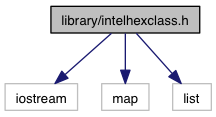
\includegraphics[width=234pt]{intelhexclass_8h__incl}
\end{center}
\end{figure}
\subsection*{Classes}
\begin{DoxyCompactItemize}
\item 
class \hyperlink{classintelhex}{intelhex}
\begin{DoxyCompactList}\small\item\em Class to decode, encode and manipulate Intel H\-E\-X format files. \end{DoxyCompactList}\end{DoxyCompactItemize}


\subsection{Detailed Description}
\begin{DoxyAuthor}{Author}
Stuart Cording aka C\-O\-D\-I\-N\-G\-H\-E\-A\-D
\end{DoxyAuthor}
A class to handle the encoding, decoding and manipulatio of an Intel H\-E\-X format file as generated by many tool chains for embedded processors and microcontrollers.

This class is constructed based upon the definition given in the document 'Hexadecimal Object File Format Specification', Revision A, January 6, 1988, © 1998 Intel Corporation.

\begin{DoxyNote}{Note}
See the git versioning notes for version information 
\end{DoxyNote}

\hypertarget{_mask_buffer_8h}{\section{library/\-Mask\-Buffer.h File Reference}
\label{_mask_buffer_8h}\index{library/\-Mask\-Buffer.\-h@{library/\-Mask\-Buffer.\-h}}
}
{\ttfamily \#include \char`\"{}Bl\-Request.\-h\char`\"{}}\\*
{\ttfamily \#include \char`\"{}crc.\-h\char`\"{}}\\*
{\ttfamily \#include \char`\"{}Wifly\-Control\-Exception.\-h\char`\"{}}\\*
\subsection*{Classes}
\begin{DoxyCompactItemize}
\item 
class \hyperlink{class_wy_light_1_1_base_buffer}{Wy\-Light\-::\-Base\-Buffer}
\item 
class \hyperlink{class_wy_light_1_1_mask_buffer}{Wy\-Light\-::\-Mask\-Buffer}
\item 
class \hyperlink{class_wy_light_1_1_unmask_buffer}{Wy\-Light\-::\-Unmask\-Buffer}
\end{DoxyCompactItemize}
\subsection*{Namespaces}
\begin{DoxyCompactItemize}
\item 
namespace \hyperlink{namespace_wy_light}{Wy\-Light}
\end{DoxyCompactItemize}

\hypertarget{_message_queue_8h}{\section{library/\-Message\-Queue.h File Reference}
\label{_message_queue_8h}\index{library/\-Message\-Queue.\-h@{library/\-Message\-Queue.\-h}}
}
{\ttfamily \#include $<$iostream$>$}\\*
{\ttfamily \#include $<$condition\-\_\-variable$>$}\\*
{\ttfamily \#include $<$thread$>$}\\*
{\ttfamily \#include $<$queue$>$}\\*
\subsection*{Classes}
\begin{DoxyCompactItemize}
\item 
class \hyperlink{class_wy_light_1_1_message_queue}{Wy\-Light\-::\-Message\-Queue$<$ T $>$}
\end{DoxyCompactItemize}
\subsection*{Namespaces}
\begin{DoxyCompactItemize}
\item 
namespace \hyperlink{namespace_wy_light}{Wy\-Light}
\end{DoxyCompactItemize}

\hypertarget{_script_8h}{\section{library/\-Script.h File Reference}
\label{_script_8h}\index{library/\-Script.\-h@{library/\-Script.\-h}}
}
{\ttfamily \#include \char`\"{}Fw\-Command.\-h\char`\"{}}\\*
{\ttfamily \#include $<$list$>$}\\*
{\ttfamily \#include $<$string$>$}\\*
{\ttfamily \#include $<$memory$>$}\\*
\subsection*{Classes}
\begin{DoxyCompactItemize}
\item 
class \hyperlink{class_wy_light_1_1_script}{Wy\-Light\-::\-Script}
\end{DoxyCompactItemize}
\subsection*{Namespaces}
\begin{DoxyCompactItemize}
\item 
namespace \hyperlink{namespace_wy_light}{Wy\-Light}
\end{DoxyCompactItemize}

\hypertarget{_telnet_proxy_8h}{\section{library/\-Telnet\-Proxy.h File Reference}
\label{_telnet_proxy_8h}\index{library/\-Telnet\-Proxy.\-h@{library/\-Telnet\-Proxy.\-h}}
}
{\ttfamily \#include \char`\"{}Client\-Socket.\-h\char`\"{}}\\*
{\ttfamily \#include \char`\"{}trace.\-h\char`\"{}}\\*
{\ttfamily \#include $<$string$>$}\\*
\subsection*{Classes}
\begin{DoxyCompactItemize}
\item 
class \hyperlink{class_wy_light_1_1_telnet_proxy}{Wy\-Light\-::\-Telnet\-Proxy}
\end{DoxyCompactItemize}
\subsection*{Namespaces}
\begin{DoxyCompactItemize}
\item 
namespace \hyperlink{namespace_wy_light}{Wy\-Light}
\end{DoxyCompactItemize}
\subsection*{Macros}
\begin{DoxyCompactItemize}
\item 
\#define \hyperlink{_telnet_proxy_8h_a2139cfcd9b3c7af8c0246e72ca4ae807}{A\-O\-K}~\char`\"{}A\-O\-K\textbackslash{}r\textbackslash{}n$<$4.\-00$>$ \char`\"{}
\item 
\#define \hyperlink{_telnet_proxy_8h_accdbea14ea06c15e271784368bd993e8}{P\-R\-O\-M\-P\-T}~\char`\"{}\textbackslash{}r\textbackslash{}n$<$4.\-00$>$ \char`\"{}
\end{DoxyCompactItemize}


\subsection{Macro Definition Documentation}
\hypertarget{_telnet_proxy_8h_a2139cfcd9b3c7af8c0246e72ca4ae807}{\index{Telnet\-Proxy.\-h@{Telnet\-Proxy.\-h}!A\-O\-K@{A\-O\-K}}
\index{A\-O\-K@{A\-O\-K}!TelnetProxy.h@{Telnet\-Proxy.\-h}}
\subsubsection[{A\-O\-K}]{\setlength{\rightskip}{0pt plus 5cm}\#define A\-O\-K~\char`\"{}A\-O\-K\textbackslash{}r\textbackslash{}n$<$4.\-00$>$ \char`\"{}}}\label{_telnet_proxy_8h_a2139cfcd9b3c7af8c0246e72ca4ae807}
\hypertarget{_telnet_proxy_8h_accdbea14ea06c15e271784368bd993e8}{\index{Telnet\-Proxy.\-h@{Telnet\-Proxy.\-h}!P\-R\-O\-M\-P\-T@{P\-R\-O\-M\-P\-T}}
\index{P\-R\-O\-M\-P\-T@{P\-R\-O\-M\-P\-T}!TelnetProxy.h@{Telnet\-Proxy.\-h}}
\subsubsection[{P\-R\-O\-M\-P\-T}]{\setlength{\rightskip}{0pt plus 5cm}\#define P\-R\-O\-M\-P\-T~\char`\"{}\textbackslash{}r\textbackslash{}n$<$4.\-00$>$ \char`\"{}}}\label{_telnet_proxy_8h_accdbea14ea06c15e271784368bd993e8}

\hypertarget{_wifly_color_8h}{\section{library/\-Wifly\-Color.h File Reference}
\label{_wifly_color_8h}\index{library/\-Wifly\-Color.\-h@{library/\-Wifly\-Color.\-h}}
}
{\ttfamily \#include $<$iostream$>$}\\*
{\ttfamily \#include $<$netinet/in.\-h$>$}\\*
{\ttfamily \#include $<$sstream$>$}\\*
{\ttfamily \#include $<$stdint.\-h$>$}\\*
\subsection*{Classes}
\begin{DoxyCompactItemize}
\item 
class \hyperlink{class_wy_light_1_1_wifly_color}{Wy\-Light\-::\-Wifly\-Color}
\end{DoxyCompactItemize}
\subsection*{Namespaces}
\begin{DoxyCompactItemize}
\item 
namespace \hyperlink{namespace_wy_light}{Wy\-Light}
\end{DoxyCompactItemize}

\hypertarget{_wifly_control_8h}{\section{library/\-Wifly\-Control.h File Reference}
\label{_wifly_control_8h}\index{library/\-Wifly\-Control.\-h@{library/\-Wifly\-Control.\-h}}
}
{\ttfamily \#include $<$string$>$}\\*
{\ttfamily \#include \char`\"{}Com\-Proxy.\-h\char`\"{}}\\*
{\ttfamily \#include \char`\"{}wifly\-\_\-cmd.\-h\char`\"{}}\\*
{\ttfamily \#include \char`\"{}Bl\-Request.\-h\char`\"{}}\\*
{\ttfamily \#include \char`\"{}Telnet\-Proxy.\-h\char`\"{}}\\*
{\ttfamily \#include \char`\"{}Wifly\-Control\-Exception.\-h\char`\"{}}\\*
{\ttfamily \#include \char`\"{}Fw\-Command.\-h\char`\"{}}\\*
{\ttfamily \#include \char`\"{}Script.\-h\char`\"{}}\\*
\subsection*{Classes}
\begin{DoxyCompactItemize}
\item 
class \hyperlink{class_wy_light_1_1_control}{Wy\-Light\-::\-Control}
\begin{DoxyCompactList}\small\item\em Class to communicate with a Wifly\-\_\-\-Light Hardware. \end{DoxyCompactList}\end{DoxyCompactItemize}
\subsection*{Namespaces}
\begin{DoxyCompactItemize}
\item 
namespace \hyperlink{namespace_wy_light}{Wy\-Light}
\end{DoxyCompactItemize}


\subsection{Detailed Description}
\begin{DoxyAuthor}{Author}
Nils Weiss, Patrick Bruenn
\end{DoxyAuthor}
! 
\hypertarget{_wifly_control_exception_8h}{\section{library/\-Wifly\-Control\-Exception.h File Reference}
\label{_wifly_control_exception_8h}\index{library/\-Wifly\-Control\-Exception.\-h@{library/\-Wifly\-Control\-Exception.\-h}}
}
{\ttfamily \#include $<$stdio.\-h$>$}\\*
{\ttfamily \#include $<$exception$>$}\\*
{\ttfamily \#include $<$string$>$}\\*
{\ttfamily \#include $<$typeinfo$>$}\\*
{\ttfamily \#include \char`\"{}wifly\-\_\-cmd.\-h\char`\"{}}\\*
{\ttfamily \#include \char`\"{}Bl\-Request.\-h\char`\"{}}\\*
\subsection*{Classes}
\begin{DoxyCompactItemize}
\item 
class \hyperlink{class_wy_light_1_1_fatal_error}{Wy\-Light\-::\-Fatal\-Error}
\item 
class \hyperlink{class_wy_light_1_1_connection_lost}{Wy\-Light\-::\-Connection\-Lost}
\item 
class \hyperlink{class_wy_light_1_1_connection_timeout}{Wy\-Light\-::\-Connection\-Timeout}
\item 
class \hyperlink{class_wy_light_1_1_invalid_parameter}{Wy\-Light\-::\-Invalid\-Parameter}
\item 
class \hyperlink{class_wy_light_1_1_script_buffer_full}{Wy\-Light\-::\-Script\-Buffer\-Full}
\end{DoxyCompactItemize}
\subsection*{Namespaces}
\begin{DoxyCompactItemize}
\item 
namespace \hyperlink{namespace_wy_light}{Wy\-Light}
\end{DoxyCompactItemize}
\subsection*{Enumerations}
\begin{DoxyCompactItemize}
\item 
enum \hyperlink{namespace_wy_light_afd625f917b07e9c48f67c4383af5773f}{Wy\-Light\-::\-Wifly\-Error} \{ \\*
\hyperlink{namespace_wy_light_afd625f917b07e9c48f67c4383af5773fa041d99db4a9cc85ed3b2682c3a4530b5}{Wy\-Light\-::\-N\-O\-\_\-\-E\-R\-R\-O\-R} = 0, 
\hyperlink{namespace_wy_light_afd625f917b07e9c48f67c4383af5773fab15784bfc61f7544f4b3bbac1817a793}{Wy\-Light\-::\-F\-A\-T\-A\-L\-\_\-\-E\-R\-R\-O\-R}, 
\hyperlink{namespace_wy_light_afd625f917b07e9c48f67c4383af5773fa507ea1a926f43bf1604d8f83ac2ce8df}{Wy\-Light\-::\-C\-O\-N\-N\-E\-C\-T\-I\-O\-N\-\_\-\-L\-O\-S\-T}, 
\hyperlink{namespace_wy_light_afd625f917b07e9c48f67c4383af5773fa66154513af88023e418086be2c270446}{Wy\-Light\-::\-C\-O\-N\-N\-E\-C\-T\-I\-O\-N\-\_\-\-T\-I\-M\-E\-O\-U\-T}, 
\\*
\hyperlink{namespace_wy_light_afd625f917b07e9c48f67c4383af5773fabafa98a04fa293fffcb58f1547cb0d3e}{Wy\-Light\-::\-I\-N\-V\-A\-L\-I\-D\-\_\-\-P\-A\-R\-A\-M\-E\-T\-E\-R}, 
\hyperlink{namespace_wy_light_afd625f917b07e9c48f67c4383af5773fa8dd025aed3813354c78e26f071501cc6}{Wy\-Light\-::\-S\-C\-R\-I\-P\-T\-\_\-\-F\-U\-L\-L}
 \}
\begin{DoxyCompactList}\small\item\em Returnvalues of Wifly\-Control\-No\-Throw. \end{DoxyCompactList}\end{DoxyCompactItemize}


\subsection{Detailed Description}
\begin{DoxyAuthor}{Author}
Nils Weiss, Patrick Bruenn 
\end{DoxyAuthor}

\hypertarget{_wifly_control_no_throw_8h}{\section{library/\-Wifly\-Control\-No\-Throw.h File Reference}
\label{_wifly_control_no_throw_8h}\index{library/\-Wifly\-Control\-No\-Throw.\-h@{library/\-Wifly\-Control\-No\-Throw.\-h}}
}
{\ttfamily \#include \char`\"{}Wifly\-Control.\-h\char`\"{}}\\*
{\ttfamily \#include $<$functional$>$}\\*
{\ttfamily \#include $<$vector$>$}\\*
\subsection*{Classes}
\begin{DoxyCompactItemize}
\item 
class \hyperlink{class_wy_light_1_1_control_no_throw}{Wy\-Light\-::\-Control\-No\-Throw}
\begin{DoxyCompactList}\small\item\em Class to communicate with a Wifly\-\_\-\-Light Hardware. \end{DoxyCompactList}\end{DoxyCompactItemize}
\subsection*{Namespaces}
\begin{DoxyCompactItemize}
\item 
namespace \hyperlink{namespace_wy_light}{Wy\-Light}
\end{DoxyCompactItemize}

\addcontentsline{toc}{part}{Index}
\printindex
\end{document}
